\documentclass[nobib,%
               a4paper,%
               notitlepage,%
%               nofonts,%
               justified]{tufte-book}
%\includeonly{sequence-learning}
\usepackage[fleqn]{amsmath}
\usepackage{mathtools}
\setlength{\mathindent}{1cm}
\usepackage{euler}
\usepackage{eulervm}
\usepackage[utf8]{inputenc}
\usepackage[group-minimum-digits=4,%
            mode=math,%
            round-mode=places,%
            round-precision=2]{siunitx}

\usepackage{enumitem}

\usepackage{tikz}
\usepackage{pgfplots}
\usepackage{pgfplotstable}
\usetikzlibrary{pgfplots.groupplots}
\pgfplotsset{compat=newest}
\usepgfplotslibrary{fillbetween,statistics,colorbrewer}
\usetikzlibrary{calc,%
                shapes,%
                backgrounds,%
                scopes,%
                shadings,%
                positioning,%\
                calendar,%
                automata,%
                decorations.pathreplacing,%
                decorations.pathmorphing,%
                angles,%
                matrix,%
                quotes,%
                external,%
}

\tikzset{
  external/mode=list and make,
  >=stealth,
  grid/.style={gray,opacity=0.2,very thin},
}
\tikzexternalize[prefix=figures/]

\usepackage[tableposition=above]{caption}

\usepackage{graphicx}
\usepackage[breakable]{tcolorbox}
%\tcbuselibrary{fitting}

\usepackage{multicol}

\usepackage[english]{babel}
\usepackage{hyperref}

\usepackage[
  type={CC},
  modifier={by},
  version={3.0},
  imagemodifier={-eu},
]{doclicense}

\usepackage{expex}
\gathertags

\usepackage{booktabs}
\usepackage{longtable}

\usepackage[framemethod=TikZ]{mdframed}
\mdfsetup{
  innerrightmargin=2cm,
  roundcorner=10pt
}
\usepackage{exsheets}
\SetupExSheets[question]{
  headings = runin,
%  pre-hook = \mdframed,
%  post-hook = \endmdframed
}

\usepackage{csquotes}
\usepackage[
  style=authoryear,
  backend=biber,
  autocite=footnote
]{biblatex}
\addbibresource{snlp.bib}

\usepackage[noend]{algpseudocode}
\usepackage{algorithm}
\usepackage{listings}

\setcounter{secnumdepth}{2}
\titleformat{\chapter}%
  {\huge\rmfamily\itshape}% format applied to label+text
  {\llap{%
			\parbox{1.5cm}{%
%				\hfill\itshape\huge\thechapter\hspace*{1ex}%
        \hfill\tikzset{external/export next=false}%
        {\tikz{\node[draw]{\itshape\huge\thechapter};}}%
				\hspace*{1ex}%
			}%
		}%
	}% label
  {0pt}% horizontal separation between label and title body
  {}% before the title body
  []% after the title body


\title{Statistical NLP: course notes}
%\date{November 10, 2016}
\author[Ç. Çöltekin]{Çağrı Çöltekin --- SfS / University of Tübingen}


\newcommand{\ra}{\ensuremath{\rightarrow}}
\newcommand{\Ra}{\ensuremath{\Rightarrow}}
\newcommand{\RA}{\ensuremath{\overset{*}{\Rightarrow}}}
\newcommand{\la}{\ensuremath{\leftarrow}}
\newcommand{\La}{\ensuremath{\Leftarrow}}

\DeclarePairedDelimiter{\norm}{\lVert}{\rVert}
\newcommand{\vect}[1]{\ensuremath{\mathbold#1}}
\newcommand{\given}{\ensuremath{\:\vert\:}}
\newcommand{\term}[1]{\emph{{#1}}}

\newcommand{\xmpl}[1]{\textit{#1}{}}
\newcommand{\xmplt}[2]{\textit{#1} `#2'{}}
\newcommand{\xmplp}[1]{/\texttt{#1}/{}}
\newcommand{\xmplpt}[2]{/\texttt{#1}/ `#2'{}}
\newcommand{\ttag}[1]{\texttt{#1}{}}

\DeclareMathOperator*{\argmin}{arg\,min}
\DeclareMathOperator*{\argmax}{arg\,max}
\usepackage{currfile}
\usepackage[draft]{snlp-notes}

\begin{document}

\frontmatter

\maketitle


\vfill
These notes are prepared for the class \emph{Statistical Natural Language Processing}
taught in Seminar für Sprachwissenschaft, University of Tübingen.

\vfill
\noindent\doclicenseLongText%
\marginnote[-2ex]{%
  \doclicenseImage%
%  \doclicenseIcon%
}
%\doclicensePlainFullText

\tableofcontents

\mainmatter
%\ifsnlpdraft
%  \fancyfoot[RE,RO]{\tiny\textcolor{gray}{Draft lecture notes. Version: \gitLastCommit @\gitLastModified;\currfilename}}
%\fi

%\chapter{Introduction}
%TODO: A good starting story, potentially involving history of NLP
%Potential resources:
% - https://blog.monkeylearn.com/the-definitive-guide-to-natural-language-processing/
%
%
% What is left for new NLP researchers/practitioners?
% (or, did google do all that can be done for NLP?)
%
% - Many languages, still few tools for majority

This is the accompanying notes
for an introductory undergraduate course on
\emph{statistical natural language processing}.
In my opinion, the modifier \emph{statistical} in the title of the course,
and these notes, is unnecessary.
The natural language processing (NLP) is necessarily statistical.
Of course we use many non-statistical components or algorithms,
but statistics (or machine learning) is a necessary component of any NLP system.
As a result, this course is a first-introduction to major concepts and applications of natural language processing.

There are already very good textbooks \parencite[notably][]{jurafsky2009,manning1999} on NLP.
This notes do not intend to replace them.
The notes follow the topics taught in the class,
and some topics discussed require other sources.
The main motivation is to provide students concise material for the students.
Having these notes also relives the instructor of trying to provide
slides that are instructive, and allows them to be more demonstrative.

\section{The plan}

The course will covers the following NLP topics and applications:

\begin{itemize}
  \item Tokenization, normalization
  \item Language models
  \item Part of speech tagging
  \item Morphology, morphological processing
  \item Probabilistic parsing
  \item Computational (vector space) semantics
  \item Word sense disambiguation
  \item Text categorization
  \item Question answering
  \item Summarization (?)
  \item Named entity recognition
  \item Information Retrieval
  \item Coreference resolution (?)
  \item Speech recognition (?)
  \item Grammar induction (?)
  \item Computational methods for linguistics and cognitive science (?)
  \item Corpora, corpus collection, annotation (?)
\end{itemize}

To be able to do get a fair understanding of these topics,
we will need some topics from mathematics,
probability theory, statistics, machine learning and linguistics.
These will be introduced (necessarily) rather superficially,
yet the introduction will be sufficient for the purposes of the course,
for most students.
Further pointers to books and resources will be provided for those
who need more material or want to learn these topic more in-depth.

\begin{itemize}
  \item Linguistic essentials
  \item Mathematical preliminaries
  \item Probability theory
  \item Statistics
  \item Information theory
  \item Machine learning basics: naive Bayes, regressing, logistic regression
  \item Bayesian learning
  \item Neural Networks
  \item Unsupervised learning
  \item The EM algorithm
  \item Unsupervised Bayesian learning
\end{itemize}


%\part{Background}
\chapter{\label{ch:math}Mathematical preliminaries}

Many methods and applications of natural language processing require
topics from mathematics.
Being an interdisciplinary field,
it is often difficult to assume
that all students of computational linguistics possess a (fresh) knowledge of
some of the mathematical topics and notation.
This chapter provides a highly coarse overview
of some topics in calculus and linear algebra.
The discussion here is incomplete and informal.
The interested reader should follow
the references provided for in-depth treatments of these subjects.

Section~\ref{sec:linear-intro} introduces some topics from linear algebra.
We will mainly introduce vectors, matrices and operations on vectors and matrices.
Again, these topics and notation will be important in discussing
many of the machine learning methods.


In Section~\ref{sec:calculus-intro},
we will very briefly revisit derivatives and integrals.
Particularly, derivatives are used for finding maxima or minima of functions,
which is the basis for many of the machine learning methods.
The integrals will also come back in our discussion of some of the machine learning methods,
particularly in discussion of probabilistic learning and inference.

\section{\label{sec:linear-intro}Linear algebra}

In many NLP methods,
we make heavy use of \term{vectors} and \emph{matrices},
which are objects studied in \emph{linear algebra}.
Vectors are used for representing \term{features} in many machine learning methods.
Operations on vectors and matrices also have important applications.
In this section we will review some of the properties of vectors and matrices,
and the operations defined on them.
If you had a linear algebra course,
of if you know, for example, matrix multiplication,
or dot product of vectors, you can safely skip this section.

\subsection{Vectors}

\begin{marginfigure}[5ex]
  \tikzsetnextfilename{vector-magnitude-direction}
  \begin{tikzpicture}
    \draw[->,thick] (0,0) -- (1, 1);
    \draw[blue,dotted] (-1,-1) -- (2, 2)
      node[near end, above,font=\scriptsize,sloped] {direction};
    \node[coordinate] (x) at ($(0.5,0)!(0,0)!(1.5,1)$) {};
    \node[coordinate] (y) at ($(0.5,0)!(1,1)!(1.5,1)$) {};
    \draw[dotted,gray]  (x) -- (0,0);
    \draw[dotted,gray]  (y) -- (1,1);
    \draw[<->,dotted,blue]  (x) -- (y)
      node[midway,below,font=\scriptsize,sloped] {magnitude};
  \end{tikzpicture}
  \caption{\label{fig:single-vector-example}A graphical representation of a vector.}
\end{marginfigure}
A vector is a mathematical object with a magnitude and a direction.
Graphically, we can represent or visualize a (two-dimensional) vector
as in Figure~\ref{fig:single-vector-example}.
More commonly,
we represent vectors by an ordered list of number,
such as $(1, 0, 1)$.
A vector defined with $n$ real numbers is said to be in the vector space $\mathbb{R}^{n}$.
We often write a vector of $n$ real numbers (vectors in $\mathbb{R}^{n}$) as
$\vect{v} = (v_{1}, v_{2}, \ldots, v_{n})$.
Note that the $\vect{v}$ that stands for the vector is typeset in boldface font.
It can alternatively be marked with a arrow over it, like $\vec{v}$.
Other notations for vectors of $n$ numbers include
$\vect{v} = \langle v_{1}, v_{2}, \ldots, v_{n}\rangle$ or
$\vect{v} = \begin{bmatrix} v_{1}\\ \vdots\\ v_{n}\\ \end{bmatrix}$.

\begin{marginfigure}[5ex]
  \tikzsetnextfilename{example-vectors}
  \begin{tikzpicture}[scale=0.7]
    \draw[<->,thick] (0, -4) -- (0, 4);
    \node[anchor=west] at (0, 4) {y};
    \draw[<->,thick] (-4, 0) -- (4, 0);
    \node[anchor=south] at (4, 0) {x};
    \draw[step=1cm,grid] (-4,-4) grid (4,4);
    \draw[thick, ->,red] (0,0) -- (1,1);
    \node[anchor=west,red] at (1,1) {$(1,1)$};
    \draw[thick, ->,blue] (0,0) -- (1,3);
    \node[anchor=west,blue] at (1,3) {$(1,3)$};
    \draw[thick, ->,green] (0,0) -- (-1,-3);
    \node[anchor=east,green] at (-1,-3) {$(-1,-3)$};
  \end{tikzpicture}
  \caption{\label{fig:vector-examples}Example vectors in 2-dimensional Euclidean space.}
\end{marginfigure}
Geometrically, we represent vectors as arrows as in Figure~\ref{fig:vector-examples}.
The individual numbers on the notation represent their projection to the respective axis.
In the example on the right,
for example,
the green and blue vectors have the same magnitude,
but their direction is opposite of each other.
If we take the projections of the vector to the $x$ and $y$ axes,
they correspond to real first and the second number in our notation respectively.

Many operations on (real) numbers have analogues forms for vectors,
and they are used in many branches of science,
as well as machine learning and natural language processing.

\newthought{Vector norms} are
a generalization of the magnitude of a vector.
A \term{norm} assigns a non-negative \emph{length} or \emph{size} to a vector.
Norms are used often in many machine learning methods,
and they are related to distance metrics which by themselves are useful in comparing objects represented as (feature) vectors.%
\footnote{The norm of a vector is the distance from its tail to its tip.}
The most familiar norm is the Euclidean norm,
which is also known as L2 (or L$^{\text{2}}$) norm.
L2 norm of a vector $\vect{v} = (v_{1}, \ldots, v_{n})$ is

\[
  \norm{\vect{v}}_{2} = \sqrt{v_{1}^{2} + \ldots + v_{n}^{2}}\;.
\]

The subscript 2\ in $\norm{v}_{2}$ communicates that the norm is L2 norm.
The L2 norm is often taken to be the default.
If the subscript is omitted then we mean the L2 norm.
Another interesting norm for our purposes is the L1 norm,
which is related to the so-called taxi-cab, city-block or Manhattan distance.
It is defined as

\[
  \norm{\vect{v}}_{1} = \lvert{}v_{1}\rvert + \ldots + \lvert{}v_{n}\rvert\;.
\]

\begin{marginfigure}[5ex]
  \tikzsetnextfilename{regularization-l1-l2}
  \begin{tikzpicture}
    \draw[step=1cm,grid] (-1,-1) grid (4,4);
    \draw[->,thick] (0, -1) -- (0, 4);
    \node[anchor=west] at (0, 4) {y};
    \draw[->,thick] (-1, 0) -- (4, 0);
    \node[anchor=south] at (4, 0) {x};
    \node[anchor=west,red] at (3,3) {$(3,3)$};
    \draw[very thick,blue] (0,0) -- (3,3);
    \draw[very thick,red,dotted] (0.05,0) -- (3,0) -- (3,0.05) -- (3,3);
    \draw[very thick,orange,dotted] (0,0) -- (0,2) -- (1,2) -- (1,3) -- (3,3);
    \draw[very thick,green,dotted]
      (0,0) -- (1,0) -- (1,1) -- (2,1) -- (2,2) -- (3, 2) -- (3,3);
  \end{tikzpicture}
  \caption{\label{fig:l1-l2}%
    Visualizations of L2(solid \textcolor{blue}{blue})
    and example L1
    (dotted \textcolor{green}{green},
            \textcolor{orange}{orange}
        and \textcolor{red}{red})
    norms vector $(3,3)$.}
\end{marginfigure}

Figure~\ref{fig:l1-l2} visualizes the L1 and L2 norms
in two-dimensional Euclidean space.
Note that both apply to higher dimensional spaces as well.
So for our example,
\[ \norm{(3,3)}_{2} = \sqrt{3^{2} + 3^{2}} = \sqrt{18} \approx 4.24\]
\[ \norm{(3,3)}_{1} = \lvert{}3\rvert + \lvert{}3\rvert = 6 \]\;.
Like any other vector operation or property,
vector norms can be generalized to vectors of any dimension.

The concept of vector norm
can also be generalized to any positive integer $p$
the L$_{\text{p}}$ norm for an n-dimensional vector is defined as

\[
  \norm{\vect{v}}_{p} = \left(
          \sum_{i=1}^{n} \lvert{}v_{i}\rvert^{p}
        \right)^\frac{1}{p}
\]

In this course, we will only work with L1 and L2 norms defined above.

\newthought{Scalar multiplication} is the operation of
multiplying a vector with a scalar
(for our purposes a scalar is a real number).
Given a vector $\vect{v} = (v_{1},\ldots, v_{n})$,
its multiplication with scalar $a$ is defined as

\[
  a \vect{v} = (a v_{1}, \ldots, a v_{2})
\]

Multiplying a vector with a positive scalar,
changes its magnitude, `scales' it,
but does not change its direction.
Multiplying a vector with a negative scalar
reverses the direction of the original vector.

\begin{marginfigure}[-5ex]
  \tikzsetnextfilename{scalar-multiplication}
  \begin{tikzpicture}[scale=0.7]
    \draw[<->,thick] (0, -4) -- (0, 4);
    \draw[<->,thick] (-4, 0) -- (4, 0);
    \draw[step=1cm,grid] (-4,-4) grid (4,4);
%          \draw[->,line width=1mm, blue!40] (0,0) -- (2,4);
    \draw[->,very thick, blue!40] (0,0) -- (2,4);
    \node[anchor=north west, blue!40] at (2,4) {$2 \vect{v}$};
    \draw[->,thick,red] (0,0) -- (1,2);
    \node[anchor=west, red] at (1,2) {$\vect{v} = (1,2)$};
    \draw[->,thick,green] (0,0) -- (-0.5,-1);
    \node[anchor=east, green] at (-0.5, -1) {$-0.5 \vect{v}$};
  \end{tikzpicture}
  \caption{\label{fig:scalar-multipl}%
    Scalar multiplication.
  }
\end{marginfigure}

\newthought{Vector addition and subtraction}
are defined on two vectors with the same dimensionality.
For $n$-dimensional vectors $\vect{v} = (v_{1}, \ldots, v_{n})$
and $\vect{w} = (w_{1}, \ldots, v_{w})$,
\[
  \vect{v} + \vect{w} = (v_{1} + w_{1} + \ldots + v_{n} + w_{n})
\]
The subtraction is simply addition with a negative vector,
\[
  \vect{v} - \vect{w} = \vect{v} + (-\vect{w}) = (v_{1} - w_{1} + \ldots + v_{n} - w_{n})
\]

\begin{marginfigure}
  \tikzsetnextfilename{vector-sum}
  \begin{tikzpicture}[scale=0.7]
    \draw[<->,thick] (0, -4) -- (0, 4);
    \draw[<->,thick] (-4, 0) -- (4, 0);
    \draw[step=1cm,grid] (-4,-4) grid (4,4);
    \draw[->,thick,red] (0,0) -- (1,2);
    \node[anchor=east, red] at (1,2) {$\vect{v}$};
    \draw[->,thick,blue] (0,0) -- (2,1);
%    \draw[->, dotted,blue] (1,2) -- (3,3);
    \draw[->, dotted,red] (2,1) -- (3,3);
    \node[anchor=west, blue] at (2,1) {$\vect{w}$};
    \draw[->, thick] (0,0) -- (3,3);
    \node[anchor=south] at (3,3) {$\vect{v + w}$};
    \draw[->,thick,purple] (0,0) -- (-2,-1);
    \draw[->,purple,dotted] (1,2) -- (-1,1);
    \node[anchor=north, purple] at (-2, -1) {$-\vect{w}$};
    \draw[->,thick,black] (0,0) -- (-1,1);
    \node[anchor=south,xshift=-0.5em] at (-1, 1) {$\vect{v}-\vect{w}$};
  \end{tikzpicture}
  \caption{\label{fig:vector-sum}%
    Vector addition and subtraction.
  }
\end{marginfigure}

\newthought{Dot product} is a very important quantity that will come up regularly in this course.
Dot product of two vectors,
$\vect{v} = (v_{1}, \ldots, v_{n})$
and $\vect{w} = (w_{1}, \ldots, v_{w})$,
is a scalar defined as:

\[
  \vect{v}\cdot\vect{w} = v_{1} \times w_{1} + \ldots + v_{n} \times w_{n}
\]

It should be emphasized that dot product yields a scalar (real number),
not a vector.
There are other vector product operations:
\emph{outer product} that we will discuss below,
and \emph{cross product} defined for vectors in $\mathbb{R}^{3}$.
Hence, without `dot' the notation $\vect{v}\vect{w}$ is ambiguous.
However, it is common to treat $k$-dimensional vectors
as $k\times{}1$ matrices for which multiplication is not ambiguous
(we discuss this notation on page~\pageref{pageref:vector-matrix-notation}.


\begin{marginfigure}
  \tikzsetnextfilename{dot-product}
  \begin{tikzpicture}[scale=0.7]
    \draw[step=1cm,grid] (-4,-4) grid (4,4);
    \draw[<->,thick] (0, -4) -- (0, 4);
    \draw[<->,thick] (-4, 0) -- (4, 0);
    \coordinate (origin) at (0,0);
    \draw[->,thick,red] (0,0) -- (2,2);
    \node[anchor=east, red] (v) at (2,2) {$\vect{v}$};
    \draw[->,thick,blue] (0,0) -- (3,1);
    \node[anchor=west, blue] (w) at (3,1) {$\vect{w}$};
    \draw[dashed] (2,2) -- (2.4, 0.8);
    \draw [decorate,decoration={brace,amplitude=7pt,mirror,raise=4pt}]
      (0,0) -- (2.4, 0.8);
    \pic [draw, "{\small $\alpha$}", angle eccentricity=1.5]
      {angle = w--origin--v};
      \node[anchor=north,rotate=20] at (1.5,-0.1) {$\norm{v}\cos\alpha$};
  \end{tikzpicture}
  \caption{\label{fig:dot-product}%
    Dot product of two vectors.
  }
\end{marginfigure}
There is an alternative way to define the dot product,
which also leads to a nice geometric interpretation.
We can calculate the dot product as

\[
  \vect{v}\cdot\vect{w} = \norm{\vect{v}}\norm{\vect{w}} \cos \alpha
\]
where $\alpha$ is the angle between the two vectors
(see Figure~\ref{fig:dot-product}).
This also allows us to interpret the dot product geometrically.
The dot product of two vectors is proportional to each vector's magnitude,
and also to the cosine of the angle between them.
Since the cosine of the angle will be larger for smaller angles,
the dot product will be larger for vectors that point to similar directions
(keeping the magnitudes constant).
The dot product of two orthogonal vectors
(vectors with a \num{90}\textdegree{} angle between them)
is \num{0}.
If the angle is larger tan \num{90}\textdegree{},
the dot product is negative.



\newthought{Cosine similarity} is a similarity measure related to dot product,
which we will often use for measuring similarities between objects of interest,
e.g., documents.
From above, we can simply write the cosine of the angle between two vectors as,

\[ \cos\alpha = \frac{\vect{v}\vect{w}}{\norm{\vect{v}}\norm{\vect{w}}} \]

Note that by dividing the vectors to their Euclidean (L2) norms,
we are scaling them to unit vectors pointing in the same direction.
As a result, cosine similarity ignores the magnitudes of the vectors.
The cosine similarity for vectors that point to the same direction is $1$
(regardless of their magnitude) and the vectors
that point exact opposite directions have a cosine similarity of $-1$.

\todo[inline]{Cross product (?)}

\subsection{Matrices}

Matrices are the second type of mathematical objects we often encounter in various NLP methods.
A matrix is simply a two-dimensional array of numbers,
which is noted as a rectangular placement of scalars.
A matrix of $n$ rows and $m$ columns is an $n \times m$ matrix.
A real-valued $n \times m$ matrix is said to be in $\mathbb{R}^{n\times m}$.
We can think about a matrix as a collection of column or row vectors.
We denote matrices with boldface capital letters, like \vect{A}.
While referring to a matrix' elements,
we subscript the element first with its row and then its column.
  \[ \vect{A} =
    \begin{bmatrix}
      a_{1,1} & a_{1,2} & a_{1,3} & \ldots & a_{1,m} \\
      a_{2,1} & a_{2,2} & a_{2,3} & \ldots & a_{2,m} \\
      \vdots  & \vdots  & \vdots  & \ddots & \vdots \\
      a_{n,1} & a_{n,2} & a_{n,3} & \ldots & a_{n,m} \\
    \end{bmatrix}
  \]

We will briefly revisit some of the operations on matrices in this section.

\newthought{Transpose of a matrix} simply replaces its rows by columns.
Transpose of a matrix $\vect{A}$ is denoted with $\vect{A}^{T}$.

\begin{center}
  If $\vect{A} = \begin{bmatrix} a & b \\ c & d \\ e & f \\ \end{bmatrix}$,
  $\vect{A}^{T} = \begin{bmatrix} a & c & e\\ b & d  & f \\ \end{bmatrix}$.
\end{center}

\newthought{Multiplication by a scalar} is also defined for matrices.
To multiply a matrix with a scalar,
each element of the matrix is multiplied by the scalar.
For example,
\[
    2 \begin{bmatrix} 2 & 1 \\ 1 & 4 \\ \end{bmatrix} =
    \begin{bmatrix}
      2\times{}2 & 2\times{}1 \\
      2\times{}1 & 2\times{}4 \\
    \end{bmatrix} =
    \begin{bmatrix}
      4 & 2 \\
      2 & 8 \\
    \end{bmatrix}
\]

\newthought{Matrix addition and subtraction} require two matrices of same dimensions.
To obtain sum (difference) of two matrices,
each element of the second matrix is added to (subtracted from)
the corresponding element of the first matrix.
For example:

  \[
      \begin{bmatrix}
        2 & 1 \\
        1 & 4 \\
      \end{bmatrix} +
      \begin{bmatrix}
        0 & 1 \\
        1 & 0 \\
      \end{bmatrix} =
      \begin{bmatrix}
        2+0 & 1+1 \\
        1+1 & 4+0 \\
      \end{bmatrix} =
      \begin{bmatrix}
        2 & 2 \\
        2 & 4 \\
      \end{bmatrix}
  \]

\newthought{Matrix multiplication} is a slightly complicated operation.
The matrix multiplication $\vect{A}\times\vect{B}$ is defined only
if \vect{A} has the same number of columns as the number of rows in \vect{B}.
Multiplying a $n\times{}k$ matrix with a $k\times{}m$ matrix
results in a $n\times{}m$ matrix.
Note that both $A\times{}B$ and $B\times{}A$ is defined only for square matrices (of the same dimensions).

For an $n\times{}k$ matrix \vect{A}
and a $k\times{}m$  \vect{B},
if $\vect{A} \times \vect{B} = \vect{C}$,
$c_{i,j}$, the element of the resulting matrix \vect{C} on row $i$ and column $j$,
is calculated as:

\[
  c_{ij} = \sum_{\ell=0}^{k} a_{i\ell} b_{\ell j}
\]

Figure~\ref{fig:matrix-mult} demonstrates the matrix multiplication.

\begin{figure*}
  \tikzsetnextfilename{matrix-multiplication}
  \begin{tikzpicture}[ampersand replacement=\&]
    \matrix (A) [matrix of math nodes,
                 left delimiter  = {[},
                 right delimiter  = {]}] at (0,0) {%
      \textcolor{blue}{a_{11}} \&
      \textcolor{blue}{a_{12}} \&
      \textcolor{blue}{\ldots} \&
      \textcolor{blue}{a_{1k}} \\
      a_{21} \&
      a_{22} \&
      \ldots \&
      a_{2k} \\
       \vdots \& \vdots \& \ddots \& \vdots \\
      a_{n1} \&
      a_{n2} \&
      \ldots \&
      a_{\textcolor{red}{nk}} \\
    };
    \node[right of=A,anchor=west,xshift=1.5cm] {\Huge$\times$};
    \matrix (B) [matrix of math nodes,
                 left delimiter  = {[},
                 right delimiter  = {]}] at (6,0) {%
      b_{11} \&
     \textcolor{blue}{b_{12}} \&
      \ldots \&
      b_{1m} \\
      b_{21} \&
      \textcolor{blue}{b_{22}} \&
      \ldots \&
      b_{2m} \\
      \vdots \&
      \textcolor{blue}{\vdots} \&
      \ddots \&
      \vdots \\
      b_{k1} \&
      \textcolor{blue}{b_{k2}} \&
      \ldots \&
      b_{\textcolor{red}{km}} \\
    };
    \node[right of=B,anchor=west,xshift=1.5cm] {\Huge$=$};
    \matrix (C) [matrix of math nodes,
                 left delimiter  = {[},
                 right delimiter  = {]}] at (12,0) {%
       c_{11} \&
       \textcolor{blue}{c_{12}} \&
       \ldots \&
       c_{1m} \\
       c_{21} \&
       c_{22} \&
       \ldots \&
       c_{2m} \\
       \vdots \&
       \vdots \&
       \ddots \&
       \vdots \\
       c_{n1} \&
       c_{n2} \&
       \ldots \&
       c_{\textcolor{red}{nm}} \\
    };
    \draw[blue]  (A-1-1.south west) rectangle (A-1-4.north east);
    \draw[blue]  (B-1-2.north west) rectangle (B-4-2.south east);
    \node[below=of C, yshift=5ex,blue]
        {$c_{12} = a_{11} b_{12} + a_{12} b_{22} + \ldots a_{1k} b_{k2}$};
  \end{tikzpicture}
  \caption{Matrix multiplication.
    The calculation of the resulting matrix \textcolor{blue}{$c_{12}$} is highlighted.
  }\label{fig:matrix-mult}
\end{figure*}

Note that the element $c_{ij}$ is the dot product of
$i^{th}$ row vector of \vect{A} and $j^{th}$ column vector of \vect{B}.
Hence, we can view dot-product as matrix multiplication
of a row vector (on the left) and column vector (on the right).
Dot product of two vectors \vect{v} and \vect{w} is often noted as
$\vect{v}\vect{w}^{T}$.%
\footnote{It is a common convention to assume that vectors are column vectors
  unless stated otherwise.}
Technically,
result of a matrix multiplication of a $1\times{}k$ vector with a $k\times{}1$
vector is a $1\times{}1$ matrix,
not a scalar.
However, this notation is prevalent in machine learning and NLP literature,
we will often use this notation during this course.

\label{pageref:vector-matrix-notation}
For example, $\vect{w} = (2, 2)$ and $\vect{v} = (2, -2)$,

\[
  \vect{v}\vect{w}^{T} = \begin{bmatrix}
    2 \\ -2 \\
  \end{bmatrix}
  \times
  \begin{bmatrix}
    2 & 2 \\
  \end{bmatrix}
  = 2\times{}2 + 2\times{}-2 = 4 - 4 = 0
\]

\marginnote{What does the result of dot product ($0$) say about the vectors?}

\newthought{Outer product} of two vectors with the same dimensionality,
can also be defined as matrix multiplication.
This time we put the column vector to the left and the row vector to the right.
So, in the notation used above, outer product of two matrices \vect{v} and \vect{w} is
$\vect{v}^{T}\vect{w}$.
Note that result of outer product of two $k$-dimensional vectors is
a $k\times{}k$ matrix, not a scalar.
The following is an example of outer product of two $3$-dimensional vectors.

\[
  \begin{bmatrix}
    1 & 2 & 3\\
  \end{bmatrix}
  \times
  \begin{bmatrix}
    6 \\ 5  \\ 4 \\
  \end{bmatrix}
  =
  \begin{bmatrix}
    6  & 5 & 4 \\
    12  & 10 & 8 \\
    18  & 15 & 12 \\
  \end{bmatrix}
\]

\todo[inline]{Relation to SVD / variance ?}

\newthought{An identity matrix} is a square matrix
in which all the elements of the main diagonal are ones,
and all other elements are zeros.
The $n\times{}n$ identity matrix is denoted by $\vect{I}_{n}$.
When there is no ambiguity, we omit the subscript, and simply write \vect{I}.
Multiplying a matrix with a compatible identity matrix does not change the original matrix.
For $n \times m$ matrix \vect{A},
\[
  \vect{I}_{n} \vect{A} = \vect{A} \quad \vect{A} \vect{I}_{m} = \vect{A}
\]

\begin{marginfigure}
  \[
    \vect{I}_{4} =
    \begin{bmatrix}
      1 & 0 & 0 & 0\\
      0 & 1 & 0 & 0\\
      0 & 0 & 1 & 0 \\
      0 & 0 & 0 & 1 \\
    \end{bmatrix}
  \]
  \caption{\label{fig:identity-matrix}$4\times{}4$ identity matrix.}
\end{marginfigure}

\newthought{Multiplying a vector with a matrix} (linearly) transforms it to another
(possibly a different dimensional) vector.
These linear transformations have many applications,
and they will also be useful for understanding some of the machine learning concepts.
Here are a few interesting transformations in 2-dimensional space:

\begin{itemize}
  \item Identity transformation has no effect on the vector to be transformed
    \[
      \begin{bmatrix}
        1 & 0 \\
        0 & 1 \\
      \end{bmatrix}
      \times
      \begin{bmatrix}
        1 \\
        2 \\
      \end{bmatrix}
      =
      \begin{bmatrix}
        1 \\
        2 \\
      \end{bmatrix}
    \]
  \item Stretch along x-axis
    \[
      \begin{bmatrix}
        3 & 0 \\
        0 & 1 \\
      \end{bmatrix}
      \times
      \begin{bmatrix}
        1 \\
        2 \\
      \end{bmatrix}
      =
      \begin{bmatrix}
        3 \\
        2 \\
      \end{bmatrix}
    \]
  \begin{marginfigure}
    \tikzsetnextfilename{linear-op-stretch}
    \begin{tikzpicture}[scale=0.7]
      \draw[step=1cm,grid] (-4,-1) grid (4,4);
      \draw[->] (0,-1) -- (0, 4);
      \draw[<->] (-4,0) -- (4,0);
      \coordinate (v1) at (1,2);
      \coordinate (v2) at (3,2);
      \draw[blue,thick,->] (0,0) -- (v1);
      \node[anchor=south east]  at (v1) {$(1,2)$};
      \draw[orange,thick,->] (0,0) -- (v2);
      \node[anchor=south west]  at (v2) {$(3,2)$};
      \draw[dotted,->,thick] (v1) to[bend left] (v2);
    \end{tikzpicture}
    \caption{Stretch (three times) along x.}
  \end{marginfigure}
  \item Multiplying a vector with
    \[
        \begin{bmatrix}
          \cos\theta & -\sin\theta \\
          \sin\theta & \cos\theta \\
        \end{bmatrix}
    \]
  rotates it with $\theta$ degrees (counter-clock wise).
  For example, for 90-dgrees rotation,
    \[
      \begin{bmatrix}
        0 & -1 \\
        1 & 0 \\
      \end{bmatrix}
      \times
      \begin{bmatrix}
        1 \\
        2 \\
      \end{bmatrix}
      =
      \begin{bmatrix}
        -2 \\
        1 \\
      \end{bmatrix}
    \]
  \begin{marginfigure}
    \tikzsetnextfilename{linear-op-rotate}
    \begin{tikzpicture}[scale=0.7]
      \draw[step=1cm,grid] (-4,-1) grid (4,4);
      \draw[->] (0,-1) -- (0, 4);
      \draw[<->] (-4,0) -- (4,0);
      \coordinate (v1) at (1,2);
      \coordinate (v2) at (-2,1);
      \draw[blue,thick,->] (0,0) -- (v1);
      \node[anchor=south west]  at (v1) {$(1,2)$};
      \draw[orange,thick,->] (0,0) -- (v2);
      \node[anchor=south east]  at (v2) {$(-2,1)$};
      \draw[dotted,->,thick] (v1) to[bend right] (v2);
    \end{tikzpicture}
    \caption{Rotate 90 degrees.}
  \end{marginfigure}
%  \item Shear: $\begin{bmatrix}1 & k \\ 0 & 1 \\\end{bmatrix}$
\end{itemize}

These linear operations can be combined (composed)
for more complex transformations.

\newthought{Solving a set of linear linear equations} has been one of
the main applications of linear algebra.
We will not discuss how to solve a linear equations here
(since we rarely do this by hand),
but we will demonstrate how a set of linear equations are represented using matrices
and vectors.
We will encounter this in various forms during the course.

The set of equations,
    \[
      \begin{array}{rcrcr}
        2x_{1} &+& x_{2}  &=& 6 \\
        x_{1}  &+& 4x_{2} &=& 17 \\
      \end{array}
    \]
    can be written as:
    \[
      \underbrace{\begin{bmatrix} 
        2 & 1 \\ 
        1 & 4 \\ 
      \end{bmatrix}}_{\vect{W}}
      \underbrace{\begin{bmatrix} 
        x_{1} \\ 
        x_{2} \\ 
      \end{bmatrix}}_{\vect{x}} 
      = 
      \underbrace{\begin{bmatrix} 
        6 \\ 
        17 \\ 
      \end{bmatrix}}_{\vect{b}}
    \]
which allows finding a solution (if one exists)
using \emph{Gaussian elimination}.

For our purposes,
important part is to realize that
this amounts to the matrix/vector operations operations
we have been reviewing so far.

\newthought{Inverse of a matrix} is defined for square matrices. 
Inverse of matrix \vect{W} is denoted by $\vect{W}^{-1}$.
Multiplying a matrix with its inverse yields the identity matrix.
\[
  \vect{W}\vect{W}^{-1} = \vect{W}^{-1} \vect{W} = \vect{I}
\]

Now that we have defined the inverse of a matrix,
we can solve the set of linear equations $\vect{W}\vect{x} = \vect{b}$,
using the inverse matrix.
\[ 
  \begin{aligned}
    \vect{W} \vect{x} &= \vect{b} \\
    \vect{W}^{-1} \vect{W} \vect{x} &= \vect{W}^{-1} \vect{b} \\
    \vect{I} \vect{x} &= \vect{W}^{-1} \vect{b} \\
    \vect{x} &= \vect{W}^{-1} \vect{b} \\
  \end{aligned}
\]

\todo[inline]{note `pseudo inverse' ?}
Calculating inverse of a matrix involves using a set of operations,
called \emph{elementary row operations},
on the augmented matrix that contains the original matrix and the identity matrix side by side.
We will not cover this here, as we rarely do this by hand.
Interested readers should check any of the linear algebra sources listed at the end of the chapter.

\newthought{The determinant of a matrix} is a scalar value
with some interesting properties and applications, including
\begin{itemize}
  \item A matrix is invertible if it has a non-zero determinant
  \item A system of linear equations has a unique solution if the coefficient matrix has a non-zero determinant
\end{itemize}

We denote the determinant of a matrix with vertical bars around it,
determinant of \vect{A} is denoted by $\lvert\vect{A}\rvert$.
Geometric interpretation of determinant is the (signed) changed in the volume of a unit (hyper)cube caused by the transformation defined by the matrix.

The determinant of a $2\times{}2$ matrix can be calculated by the formula:
\[
  \begin{vmatrix}
    a & b \\
    c & d \\
  \end{vmatrix} = a d - b c
\]
The above formula generalizes to higher dimensional matrices through a recursive definition.
\todo{definition, geometric interpretation}

\newthought{Eigenvalues and eigenvectors} of a matrix also has important applications.

An \emph{eigenvector}, \vect{v}
and corresponding \emph{eigenvalue}, $\lambda$,
of a matrix $\vect{A}$ is defined such that
\[ \vect{A} \vect{v} = \lambda \vect{v}\;. \] 

In (other) words, multiplying a matrix with its eigen vector
only changes its magnitude of the vector
and does not change its direction.

Eigenvalues an eigenvectors have many applications from communication theory to quantum mechanics
A better known example (and close to home) is Google's PageRank algorithm
We will return to them while discussing PCA
and SVD (and maybe other topics/concepts)

\todo[inline]{Tensors}

\section{\label{sec:calculus-intro}Derivatives and integrals}

Differentiation and integration are two fundamental concepts in calculus.
The reason we review some of the basic calculus here has to do
with the fact that these operations are often used
in probability theory and machine learning.
In many machine learning problems,
learning is achieved through minimizing the error
or maximizing an objective (e.g., likelihood).
A particularly important use of derivatives in machine learning is
to find maxima or minima of error or objective function.
This section will give a refresher on these topics,
and define some notation that we will use throughout the course. 
You can safely skip this section,
if you know how to differentiate polynomial functions
or what a \emph{gradient} is.

Derivative of a function indicates the rate of change.
The familiar example from physics is that
the derivative of the velocity of a moving object is it acceleration.
For example,
the velocity of a car changes proportional to its acceleration of deceleration.

\marginnote{
  \begin{tcolorbox}[colback=white,colframe=gray,halign=left,width=\linewidth]
    A quick refresher on polynomial functions: if $f(x) = x^{n}$,
    \[
      f'(x) = \frac{df}{dx}  = n x^{n-1}\;.
    \]
    For example, for\\
      $f(x) = x^{3} + 2 x^{2}$,
    \[
      f'(x) = \frac{df}{dx} = 3 x^{2} + 4 x\;.
    \]
  \end{tcolorbox}
}
One of the common ways of denoting a function's derivative is,
using the `prime notation'.
For example derivative of the function function $f(x)$ written as $f'(x)$.
Another common notation is $\frac{df}{dx}(x)$ or $\frac{df}{dx}(x)$.\todo{double check}
For multi-variate functions,
this notation makes it clear that the derivative is taken with respect to the variable $x$.

If defined, derivative of a function is another function.
A well known example is the polynomials,
whose derivatives are lower degree polynomials.
For example, if $f(x) = x^{2} - 2 x $ then $f'(x) = 2 x - 2$,
which means that the rate of change of a quadratic function doubles
as $x$ is increased one unit.
Note that if a polynomial of degree $n$ is differentiated $n$ times,
it becomes a constant.
Derivative of a linear function is a constant value,
since a linear function changes with the same rate everywhere.
On the other hand, derivative of a constant (function) is $0$,
since there is no change.

\begin{marginfigure}
  \tikzsetnextfilename{func-derivative}
  \begin{tikzpicture}[scale=0.7]
    \draw[step=1cm,grid] (-4,-2) grid (4,4);
    \draw[->] (0,-2) -- (0, 4);
    \draw[<->] (-4,0) -- (4,0);
    \begin{scope}
      \clip(-4,-2) rectangle (4,4);
      \draw[domain=-2:4,smooth,variable=\x,blue]
        plot ({\x},{\x*\x - 2*\x});

      \node[blue,xshift=0.2ex] at (1,2) {$f(x) = x^{2} - 2x$};

      \node[orange,inner sep=0pt,draw,circle,minimum size=2pt]
        at (1,-1) {};
      \node[orange,anchor=north] at (1,-1) {$f'(1) = 0$};
      \draw[orange] (-4,-1) -- (4, -1);

      \begin{scope}
      \clip(-4,-0.5) rectangle (4,4);
        \node[purple,inner sep=0pt,draw,circle,minimum size=2pt]
          at (3,3) {};
        \node[purple,anchor=south east] at (3,3) {$f'(3) = 4$};
        \draw[purple] (4, 7) -- (3,3) -- (2, -1);

        \node[red,inner sep=0pt,draw,circle,minimum size=2pt]
          at (-0.5,1.25) {};
        \draw[red] (-1.5, 4.25) -- (-0.5,1.25) -- (0.5, -1.75);
        \node[red,anchor=north east] at (-0.5,1.25) {$f'(-0.5) = -3$};
      \end{scope}
    \end{scope}
  \end{tikzpicture}
  \caption{The function $f(x) = x^{2} - 2x$ and its derivative evaluated at,
    different $x$ values.
  }
\end{marginfigure}
When evaluated at a particular $x$ value,
the derivative of the function will be
the slope of the tangent line at that point,
which is indication of the direction and the rate of change.
Note that in our example above,
the derivative of $f(x) = x^{2} - 2x$, $f'(x) = 2 x - 2$,  at $x = 1$ is $0$.
For a continuous function the derivative of the function is equal to $0$,
only on the maximum and minimum points of the function.
And this is the most important reason for all the earlier
notes in this introduction.
In many methods we see later on,
we will be aiming at maximizing or minimizing functions,
where this will be a handy tool.
In general,
derivative evaluated at a particular point will be $0$ for maxima and minima
of functions,
it will be a negative value if the function is decreasing (as $x$ increases),
and a positive value if the function is increasing with $x$.

So far,
we've considered differentiation of functions of a single variables.
In machine learning and NLP,
we often deal with functions of many variables.
One can also differentiate a function of multiple variables with respect to one of them,
for which the dependence between the variables should be considered.
We will not review how to take (total) derivatives
of functions of multiple variables.
However, we will introduce \term{partial derivatives} briefly here.
A partial derivative is similar to a total derivative,
but we assume that except the variable along which we take the derivative,
all other variables are constants.
So, when you evaluate the partial derivative of a function at a particular point,
it gives you the rate of change along one of the axes.

\todo[inline]{note the chain rule and the relation between partial/total derivative?}
The partial derivative of a function $f$ with respect variable $x$ is denoted by $\frac{\partial f}{\partial x}$.
For example, if $f(x, y) = x^{3} + yx$, 
\[
  \frac{\partial f}{\partial x}  = 3 x^{2} + y,\; \text{and}\; 
  \frac{\partial f}{\partial y}  = x .
\]
The vector formed by all partial derivatives
of a (scalar) function of $n$-variables is called its \term{gradient}.
Gradient of a function $f$ is denoted by $\nabla f$, or $\vec{\nabla} f$.
\[
  \nabla f(x_{1}, \ldots, x_{n}) = 
        \left(\frac{\partial f}{\partial x_{1}}, \ldots,
              \frac{\partial f}{\partial x_{n}} \right)
\]
Similar to derivative of a function of a single variable,
gradient points to the direction of greatest change,
and the magnitude of the gradient indicates the steepness of the change.
Areas where the gradient is \num{0} are (local) minima, maxima and saddle points.
As a result, it is an important tool
in finding minimum and maximum values of (objective) functions.

\todo[inline]{Second derivative, picture with a saddle point, Jacobian matrix(?)}


\begin{marginfigure}[-5\baselineskip]
  \tikzsetnextfilename{integration}
  \begin{tikzpicture}[x=10mm, y=2mm, scale=0.7]
    \draw[step=1cm,grid] (-4,-2) grid (4,30);
    \clip(-4,-2) rectangle (4,30);
    \draw[->] (0,-2) -- (0, 30);
    \draw[<->] (-4,0) -- (4,0);

     \draw[domain=-4:4,smooth,variable=\x,blue]
       plot ({\x},{3*\x*\x});
      \fill[blue,opacity=0.2] 
        plot[domain=1:3,smooth,variable=\x] ({\x},{3*\x*\x}) 
        -- (3,0) -- (1,0) -- cycle;
%        plot coordinates {(3,27) (3,0) (1,0) (1,3) };
  \end{tikzpicture}
  \caption{\label{fig:integral}%
    Integral of the function $f(x) = 3 x^{2}$ in range $[1, 3]$.
  }
\end{marginfigure}
\newthought{Integration} is the inverse of the derivation.
In general, the integral of a function in a given range corresponds
to the (signed) area (or volume) under a function in this range.
The notation used for integral of a function $f(x)$ is
$F(x) = \int f(x) dx$.
This is called an indefinite integral.
Often we want the integral of a function in an interval $[a,b]$,
which can be calculated by
\[
  \int_{a}^{b} f(x) dx = F(b) - F(a).
\]

For example, if $f(x) = 3 x^{2}$,
we know that $F(x) = x^{3}$ (since the integral is the antiderivative,
and $F'(x) = f(x) = 3 x^{2}$).
If we want to know the area under $f(x)$ within range $[1, 3]$,
we simply calculate $F(1) - F(0) = 27 - 1 = 26$.

\begin{marginfigure}
  \tikzsetnextfilename{numeric-integral1}
  \begin{tikzpicture}[x=10mm, y=5mm]
    \draw[step=1cm,grid] (-0.2,-0.2) grid (4,4);
    \clip(-0.2,-0.2) rectangle (4,4);
    \draw[->] (0,-0.2) -- (0, 4);
    \draw[->] (-0.2,0) -- (4,0);

     \draw[domain=-4:4,smooth,variable=\x,blue]
       plot ({\x},{0.25*\x*\x});
     \foreach \x in {1,...,6}{%
       \fill[draw=black,blue,opacity=0.2]
        (0.5*\x, 0.25*0.25*\x*\x) rectangle ($ (0.5*\x,0) + (-1*0.5, 0)$);
     }
  \end{tikzpicture}\\
  \tikzsetnextfilename{numeric-integral2}%
  \begin{tikzpicture}[x=10mm, y=5mm]
    \draw[step=1cm,grid] (-0.2,-0.2) grid (4,4);
    \clip(-0.2,-0.2) rectangle (4,4);
    \draw[->] (0,-0.2) -- (0, 4);
    \draw[->] (-0.2,0) -- (4,0);

     \draw[domain=-4:4,smooth,variable=\x,blue]
       plot ({\x},{0.25*\x*\x});
     \foreach \x in {1,...,20}{%
       \fill[draw=black,blue,opacity=0.2]
        (3*0.05*\x, 9*0.0025*0.25*\x*\x) rectangle ($ (3*0.05*\x,0) + (-1*3*0.05, 0)$);
     }
  \end{tikzpicture}
  \caption{\label{fig:ingegral-numeric}%
    Demonstration of numerical approximation to an integral.
    Note that as the rectangles get smaller (as in the figure below),
    sum of their areas gets closer to the area under the curve.
  }
\end{marginfigure}
Often integrating functions analytically
(in closed form) is not easy or possible.
In these cases, integrals can be computed with numeric approximation.
One way to do this is to sum the areas of rectangles
as demonstrated in Figure~\ref{fig:ingegral-numeric}.
As we decrease the width of the rectangles,
or equivalently, increase the number of rectangles in a fixed range,
the approximation will be more precise.
This also hints at interpreting integrals as a infinite sum.
This interpretation will often be more useful
for the examples we will see (often in probability theory).

\section*{Summary}

In this lecture,
we reviewed some concepts from linear algebra and calculus.
The aim was to
provide a refresher for those who studied these topics,
familiarize the reader with the notation that will be used,
and also give a feeling of the what mathematical concepts will be useful
for studying statistical natural language processing.
This overview here is necessarily informal and incomplete.
Below, a number of potential sources are listed if you need a better introduction to these concepts.

For linear algebra,
\textcite{cherney2013} and \textcite{beezer2016} are
two textbooks that are freely available online.
A classic reference textbook for linear algebra is \textcite{strang2009}.
For a more practical/geometric approach,
see \textcite{farin2014} or \textcite{shifrin2011}.

For the concepts we reviewed briefly from calculus,
any textbook introduction to calculus should be sufficient.
A well-known (also available online) textbook is \textcite{strang1991}.
For more alternatives on open textbooks on mathematics see
\url{http://www.openculture.com/free-math-textbooks}.

\chapter{\label{chap:prob}Probability theory}

%
% Visualizations from 
% <http://colah.github.io/posts/2015-09-Visual-Information/>
% may be useful.
%
% Add Simpson paradox, either here, or especially in statistics.


% TODO: an intro - maybe with Chomsky quote.

% Human language is probabilistic.
% This is not to say that, it is random,
% but analyzing (or comprehending) natural languages require making inferences under uncertainty.
% Take the following well-known ambiguous sentence.
% \pex
% \begingl
%   \gla We saw her duck with a telescope.//
% \endgl
% \xe
% This sentence is ambiguous in quite a few ways.%
% \sidenote{Try to list all possible interpretations of the sentence.} 
% However, even without further context,
% humans tend to prefer certain interpretations,
% to the extent that some of the interpretations are difficult to enumerate.
% The best solutions we know for 
% finding the most plausible interpretation of such sentences are 
% based on statistical methods,
% where probability theory plays a very important role.

In this chapter,
we will review some of the basic concepts from the probability theory.
% TODO: detailed listing of what comes next

The concepts introduced in this chapter will be
very important in many of the subjects
we will cover during the course.
Like the other background chapters,
you may skip this chapter if you are familiar with the probability theory.

\section{Axioms of the probability}

Probability is a measure of (un)certainty of an event.
In daily usage,
we often associate some events with some probabilities.
We talk about high- or low-probability events,
or sometimes we express our notion of probability
(loosely) by percentages or odds.

Formally,
we quantify the probability an event
with a number between \num{0} and \num{1}.
An event with probability of \num{0} is impossible,
and an event with probability of \num{1} happens with certainty.
Otherwise, any number in between,
expresses the certainty we associate with the occurrence of the event.
For example,
an event with probability of \num{0.5} is as likely to happen as it may not.

The events we talk about are outcomes of trials
(some sort of experiment or observation).
In general, an event is a set of outcomes.
The set of all possible outcomes of a trial is called its sample space,
and conventionally indicated by the Greek letter omega ($\Omega$).

Formally, probabilities has to follow the following set of axioms.

\begin{enumerate}
  \item $P(E) \in \mathbb{R}$, $P(E) \ge 0$.
    Probability of an event $E$ has to be a positive number.
  \item $P(\Omega) = 1$.
    The probability of all possible outcomes of a trial is one.
    Note that this also means that 
    probability of no event can be larger than $1$.
  \item For two \emph{disjoint} events $E_{1}$ and $E_{2}$, 
    $P(E_{1}\cup{}E_{2}) = P(E_{1}) + P(E_{2})$.
    In general, for $N$ disjoint events.
    $P(E_{1}\cup\ldots\cup E_{N} = \sum_{i=1}^{N} P(E_{i})$.
\end{enumerate}

The above three axioms forms the basis of all probabilistic statements.
The other rules that we will discuss later on can all be derived from these three rules.
Note that these axioms,
hence the probability theory,
defines only how to use or manipulate the probabilities.
It does not specify how to obtain probabilities.
There are different schools of thought that assign probabilities to events
using (somewhat) incompatible ways.
Since uncertainty, hence probability,
plays an important role in any statistical study,
we will encounter some of these differences during the course of this course.

\section{Random variables}

The concept of \term{random variable} is central to the probability theory.
The value of a random variable is subject to uncertainties.%
\footnote{
  Although,
  the value of a \emph{random variable} is not necessarily unpredictable,
  as in the typical daily use of the term `random'.
  Most random variables we study involve some uncertainties,
  but also some regularities or structure that we can exploit
  for making inferences.
  Somewhat surprisingly,
  even some aspects of a `truly random' processes include these tendencies,
  which is very important for machine learning,
  and \emph{statistical inference} in general.
}
The value of a random variable depend on the outcome of a set of random events. 
For example, we are often interested in studying outcomes
of experiments or observations that involve uncertainty such as

\begin{itemize}
  \item height or weight of a person selected (randomly) form a population
  \item length of a randomly chosen corpus
  \item whether an email is spam or not
  \item the first word of a book, or the first word uttered by a baby
\end{itemize}

In this context,
we can think of a random variable as a (well-defined) function
from the set of outcomes ($\Omega$) of an experiment to real numbers.
Clearly,
the outcome of some of these trials are not trivial to express as a real number.
Often, for mathematical convenience,
an arbitrary mapping may used,
e.g., from a set of words to consecutive integers.
However,
some of the useful quantities
(e.g., expected value or variance) does only make sense
for random events for which a meaningful mapping to the (real) numbers exists.
For example, we can define random variables whose values are
words or syntactic representations of sentences (trees),
but, in these cases quantities like mean will not be useful
(What is the average word?).%
\footnote{%
  Technically, a random variable takes real numbers.
  A more correct term used for non-numeric random variables is \emph{random element}.
  We will be using the term random variable for both cases.
}
Note that the values of random variables are not probabilities,
Probabilities are associated with the outcomes of the random experiment.

Mapping some outcomes to numbers is easy,
for example, if we are measuring the frequency of a sound signal,
or counting the number of words in a document,
the measurement already gives us a real value.
The mapping may not be trivial in some other cases,
such as whether the random variable representing
a product review is positive or negative,
or part of speech of a word.
In these cases,
there are often conventional methods for mapping these outcomes to numbers.
For example,
the Boolean variables (such as binary outcome of a review)
are typically mapped to \num{0} and \num{1} for negative and positive outcomes respectively.


For trials having outcomes with more than two categories
(as in our part of speech example),
a possible solution is to map them to integers arbitrarily,
for example,
as on the row labeled `Integer` in Table~\ref{tbl:nominal-repr}.
\begin{table}
  \begin{tabular}{lrrrrr}
    \toprule
    Part of speech            & Noun & Verb  & Adjective  & Adverb & \ldots \\
    \midrule
    Integer       & \num{1} & \num{2}  & \num{3}  & \num{4} & \ldots \\
    Binary vector &\num[minimum-integer-digits=6,group-digits=false]{1}
                  &\num[minimum-integer-digits=6,group-digits=false]{10}
                  &\num[minimum-integer-digits=6,group-digits=false]{100}
                  &\num[minimum-integer-digits=6,group-digits=false]{1000}
                  &\ldots \\
    \bottomrule
  \end{tabular}
  \caption{
    Alternative numeric representations for categorical (nominal) variables.
  }\label{tbl:nominal-repr}%
\end{table}

However, there is another method that is more convenient for many purposes.
Instead,
we map each outcome to a vector of binary (\num{0} or \num{1}) values,
where we set only a particular member of the vector to $1$,
and we set the rest to \num{0} for a particular outcome.
This representation is called \term{one-of-k} or \term{one-hot} representation,
and exemplified on the row labeled `Binary vector' in Table~\ref{tbl:nominal-repr}.
\label{desc:one-hot}
In statistical literature it is also called \term{dummy coding}.%
\footnote{%
  Note that the coding as we describe here is somewhat redundant.
  We can be slightly more economical by mapping
  one of the outcomes to all zeros.
  Although this economy is not really useful for many purposes,
  it is sometimes used (especially in statistics)
  when one of the outcomes is a special base case (coded as all zeros).
  This makes comparison of other outcomes to the base case easier.
}
This particular representation is used quite often in machine learning
while encoding categorical features.
For example whether a particular word (out of all words in a dictionary)
occurs in a document or not.%
\footnote{%
  If the outcomes/items (such as words) represented have some features
  in common,
  we can even use real values (rather than binary one-hot) in these vectors.
  We will later discuss such `dense' representations.
}

In the discussion above,
we implicitly made a distinction between two types of random variables.
Some random variables are continuous,
they can take any real number as values
(such as height or frequency).
Others, on the other hand, have discrete values.
For example,
number of words in a document or sentence can only take integer values,
and whether a document is spam or not can have only two values (true or false).
This distinction between the continuous
and categorical random variables is important, in general,
and in our discussion of some important properties
and specific distributions of random variables below.

To make the discussion more concrete,
we will use an example hypothetical random variable.
Assume that predicting the length of utterances
in a (particular type of) dialog is important for our purposes.
So, our random variable, $X$, is a discrete variable,
taking only integer values (length of utterances).
For simplicity,
we will also assume that the longest possible utterance is \num{11} words.
\begin{margintable}
  \caption{\label{tbl:prob-table}%
    Probabilities of all possible values ($x$)
    of an example random variable $X$ (utterance lengths).
  }
  \begin{center}
    \begin{tabular}{lS[round-precision=3]}
      \toprule
      $x$ & {$P(X = x)$} \\
      \midrule
      1&0.1554647600\\
      2&0.1847803882\\
      3&0.2098059244\\
      4&0.1990806945\\
      5&0.1022471910\\
      6&0.0655771195\\
      7&0.0390194076\\
      8&0.0228804903\\
      9&0.0115423902\\
     10&0.0053115424\\
     11&0.0042900919\\
      \bottomrule
    \end{tabular}
  \end{center}
\end{margintable}
Table~\ref{tbl:prob-table} lists each possible value of $X$,
with its associated probability.
Note that, in our example, $X$ is the random variable,
and $x$ is a possible value.
The first row of Table~\ref{tbl:prob-table} shows the $P(X=1)$,
whose probability turns out to be \num[round-precision=3]{0.1554647600}.
For now, we do not ask where these probabilities come from.%
\footnote{They are \emph{estimated} from a real corpus of spoken language,
but we will delay the details for now.
}
However,
it is important to note that the probabilities in the table sum to $1$
(except for potential rounding error).

In our utterance-length example (in Table~\ref{tbl:prob-table}),
there is a natural mapping between the utterance length
and the value of the random variable.
The value of the random variable is simply the integer
that corresponds to the utterance length in words.
This mapping is not always straightforward.
To demonstrate that we will give another hypothetical example
in Table~\ref{tbl:prob-table-letters}.
\begin{margintable}
  \caption{\label{tbl:prob-table-letters}%
    Probability distribution of variable $X$,
    associated with letter probabilities.
    Note that the mapping between the letters
    and the values of the random variable $x$ is arbitrary.
  }
  \begin{center}
    \begin{tabular}{lSS[round-precision=3]}
      \toprule
      letter & $x$ & {$P(X = x)$} \\
      \midrule
      a & 1&0.2330012\\
      b & 2&0.0424207\\
      c & 3&0.0464163\\
      d & 4&0.0841186\\
      e & 5&0.2859216\\
      f & 6&0.0262472\\
      g & 7&0.0633547\\
      h & 8&0.2185197\\
      \bottomrule
    \end{tabular}
  \end{center}
\end{margintable}
We assume that we are working on an ancient language,
which is written only with eight letters.
The random variable (we will use $X$ again) this time maps
the relationship between the event (observing a particular the letter) and
the value of the random variable ($x$) is more arbitrary

In both examples above,
we specified probability of a particular value of a random variable like $P(X=x)$,
for example $P(X=1)$
in Table~\ref{tbl:prob-table-letters} is \num{0.2330012}.
However, when there is no ambiguity,
we will skip the name of the random variable and write, for example,
$P(1) = \num{0.2330012}$, or even $P(\text{a}) = \num{0.2330012}$.

\subsection{Probability mass function}

\begin{marginfigure}[4ex]
  \tikzsetnextfilename{prob-mass-func},
  \begin{tikzpicture}[x=3.8mm,y=10cm]
    \foreach \x/\y in {1/0.1554647600,
                       2/0.1847803882,
                       3/0.2098059244,
                       4/0.1990806945,
                       5/0.1022471910,
                       6/0.0655771195,
                       7/0.0390194076,
                       8/0.0228804903,
                       9/0.0115423902,
                      10/0.0053115424,
                      11/0.0042900919}%
    {
      \draw[fill=blue!20]
        ($ (\x,0) + (-0.4, 0) $) rectangle ($ (\x,\y) + (0.4, 0) $);
      \node[anchor=north,font=\scriptsize] at (\x, 0) {\x};
      \draw[thick] (0.4,0) -- (0.4, 0.25);
      \foreach \i in {0, 0.05, 0.1, 0.15, 0.20, 0.25}{%
        \draw (0.4,\i) -- ++(-0.2, 0);
      }
      \foreach \i in {0, 0.1, 0.2}{%
        \node[anchor=east,font=\scriptsize] at (0.2,\i) 
          {\num[round-precision=1]{\i}};
      }
    }
  \end{tikzpicture}
  \caption{\label{fig:pmf}Graphical representation of probability mass function defined in Table~\ref{tbl:prob-table}.}
\end{marginfigure}
\emph{Probability mass function} (PMF) is a function that maps
the values of a discrete random variable to their probabilities.
The PMF of a random variable maps all possible values of the random variable
to exact probability of the associated event.
For example, probability of
an utterance of length \num{3} is \num{0.21} in our example (Table~\ref{tbl:prob-table}).
A probability mass function defines a discrete probability distribution.
Table~\ref{tbl:prob-table} defines such a PMF,
which is shown graphically in Figure~\ref{fig:pmf}.

\subsection{Probability density function}

Continuous random variables do not have probability mass functions,
but analogously they can be defined through
a \emph{probability distribution function} (PDF).
For continuous distributions,
the probability of a single value of the random variable is zero.
We can only talk about non-zero probabilities of intervals.
This may be unintuitive at first thought.
However, if you consider the fact that there are infinite number of real numbers
between any arbitrary range $[a, b]$ ($a \ne b$),
probability of any single value is statistically equivalent to zero.

% approximate gamma function declaration from:
% http://tex.stackexchange.com/questions/120441/plot-the-probability-density-function-of-the-gamma-distribution
\begin{marginfigure}
  \tikzsetnextfilename{prob-density}
  \begin{tikzpicture}[
      declare function={%
        gamma(\z)= (2.506628274631*sqrt(1/\z) +%
                    0.20888568*(1/\z)^(1.5) +%
                    0.00870357*(1/\z)^(2.5) -%
                    (174.2106599*(1/\z)^(3.5))/25920 -%
                    (715.6423511*(1/\z)^(4.5))/1244160%
                   )*exp((-ln(1/\z)-1)*\z);
      },
      declare function={%
        gammapdf(\x,\k,\theta) = \x^(\k-1)*exp(-\x/\theta) /%
                                (\theta^\k*gamma(\k));%
      }
  ]

      \begin{axis}[axis lines=left,
          enlargelimits=upper,
          samples=50,
          x=15mm,
          y=20mm,
      ]
          \addplot[smooth, thick, blue, domain=0:2.5,name path=curve]
            {gammapdf(x,3,0.2)};
          \addplot[draw=none, domain=0:2.5,name path=xax] {0};
          \addplot[blue,opacity=0.2]
            fill between[of=curve and xax,soft clip={domain=0:2.5}];
          \addplot[blue,opacity=0.4]
            fill between[of=curve and xax,soft clip={domain=1:1.5}];

      \end{axis}
%        \draw[domain=0:3,smooth,variable=\x]
%                plot (\x,{gammapdf(\x,3,0.2)});
  \end{tikzpicture}
  \caption{\label{fig:pdf}Example probability density function (PDF).
    Area under the whole curve, potentially stretching to infinity,
    is \num{1} units.
    The area under a particular interval is the probability
    that the random variable takes a value within the interval.
  }
\end{marginfigure}
As an example of a continuous random variable,
suppose we were measuring the durations of the utterances
rather than the number of words as in our discrete random variable example,
we cannot assign a non-zero probability to 
an utterance being \SI{1.4}{\second}.
However, we can assign a probability to a range,
say between \SI{1.2}{\second} and \SI{1.6}{\second}.
As a result,
the values of a PDF are not probabilities.
Figure~\ref{fig:pdf} shows a probability density function.
For the sake of demonstration,
we will pretend this to be the distribution of durations of utterances
in a spoken language corpus.
The plot actually shows a well-known density function.
Precisely, this is the probability density function of
the gamma distribution with parameters $k=3$, $\theta=0.2$,
but this is not important for this introduction.
Figure~\ref{fig:pdf} clearly shows that
the values of the PDF are not probabilities.
For example, the value corresponding to \num{0.5} is grater than \num{1}.
Another important property of the PDF,
more difficult measure from the figure,
is that the area under the curve is \num{1} unit.
Although probabilities of individual real numbers are zero,
we can calculate the probabilities of ranges,
like the one highlighted in Figure~\ref{fig:pdf}.
The probability is simply the definite integral of the PDF
in the interval we are interested in.
In this respect,
the PDF has a very similar function to probability mass function.
However,
we should not forget that the values of a PDF are not probabilities.%
\sidenote[][-10ex]{
%  \begin{tcolorbox}[colback=white,colframe=gray,halign=left,width=\linewidth]
    A common convention for distinguishing,
    a PMF from a PDF is using
    uppercase $P()$ for the former and lowercase $p()$ for tha latter.
    $P(X=x)$ yields the probability of discrete random variable being $x$,
    but the values returned by $p()$ are not probabilities,
    although higher values will indicate neighborhoods
    of high probability density.
%  \end{tcolorbox}
}

We will give brief descriptions
of some of the important continuous probability distributions
later in this chapter.

\subsection{Cumulative distribution function}

\begin{margintable}
  \caption{\label{tbl:cdf}%
    The values of \emph{probability mass function} (column 2)
    and  \emph{cumulative distribution function} (column 3)
    of the earlier example random variable, $X$, presented
    in Table~\ref{tbl:prob-table}.
  }
  \begin{center}
    \begin{tabular}{lS[round-precision=3]S[round-precision=3]}
      \toprule
      $x$ & {$P(X = x)$} & {$P(X \le x)$}\\
      \midrule
      1& 0.1554647600 & 0.1554647600\\
      2& 0.1847803882 & 0.3402451482\\
      3& 0.2098059244 & 0.5500510726\\
      4& 0.1990806945 & 0.7491317671\\
      5& 0.1022471910 & 0.8513789581\\
      6& 0.0655771195 & 0.9169560776\\
      7& 0.0390194076 & 0.9559754852\\
      8& 0.0228804903 & 0.9788559755\\
      9& 0.0115423902 & 0.9903983657\\
     10& 0.0053115424 & 0.9957099081\\
     11& 0.0042900919 & 1.0000000000\\
      \bottomrule
    \end{tabular}
  \end{center}
\end{margintable}
\emph{Cumulative distribution function} (CDF),
or \emph{distribution function} of a random variable $X$,
$F_{X}(x)$, yields the probability that $X$ will take a value
less than or equal to $x$.
\[
  F_{X}(x) = P(X \le x)
\]
In case of discrete distributions,
it is simply the sum of probabilities of all values up to and including $x$.
And, for continuous distributions,
it is the area of under the probability density function
in interval $[-\infty, x]$.
As may you have already guessed,
to evaluate the value of the CDF of a continuous random variable,
we need to integrate the PDF in this range
instead of summing.
Output of a CDF is a probability
regardless of whether the random variable is continuous or discrete.
The cumulative distribution function plays an important role
in statistics, particularly in hypothesis testing.

Table~\ref{tbl:cdf} repeats the probability mass function from
Table~\ref{tbl:prob-table} (in column 2),
and also shows the values cumulative distribution function.
Note that the CDF converges to \num[round-precision=1]{1.0}
at the maximum value of the random variable $X$.

\begin{marginfigure}
  \tikzsetnextfilename{porb-cdf}
  \begin{tikzpicture}[x=3.8mm,y=25mm]
    \foreach \x/\y in {1/0.1554647600,
                       2/0.3402451482,
                       3/0.5500510726,
                       4/0.7491317671,
                       5/0.8513789581,
                       6/0.9169560776,
                       7/0.9559754852,
                       8/0.9788559755,
                       9/0.9903983657,
                      10/0.9957099081,
                      11/1.0000000000}%
    {
      \draw[fill=blue!20]
        ($ (\x,0) + (-0.4, 0) $) rectangle ($ (\x,\y) + (0.4, 0) $);
      \node[anchor=north,font=\scriptsize] at (\x, 0) {\x};
      \draw[thick] (0.4,0) -- (0.4, 1);
      \foreach \i in {0, ..., 10}{%
        \draw (0.4,\i/10) -- ++(-0.2, 0);
      }
      \foreach \i in {0, 0.5, 1.0}{%
        \node[anchor=east,font=\scriptsize] at (0.2,\i) 
          {\num[round-precision=1]{\i}};
      }
    }
  \end{tikzpicture}
  \caption{\label{fig:cdf}Graphical representation
  of cumulative distribution function defined in Table~\ref{tbl:cdf}.}
\end{marginfigure}

\subsection{\label{ssec:expected-value}Expected value}

Expected value of a random variable is its arithmetic mean ($\mu$).
Given a list of numbers,
their arithmetic mean is simply their sum divided
by the total number of numbers in the list.
Assume that we have the following numbers,
say as the length of utterances of interest
in a (small) spoken language corpus:
\begin{center}
  \num{1},
  \num{2},
  \num{3}, \num{3}, \num{3},
  \num{4}, \num{4},
  \num{5},
  \num{7},
  \num{11}
\end{center}
To find the arithmetic mean,
we simply sum these numbers up, and divide the number of items in our list.
Which gives us \num[round-precision=1]{4.3}. 
\begin{marginfigure}
  \tikzsetnextfilename{histogram-mean}
  \begin{tikzpicture}[x=4mm,y=5mm]
    \foreach \x/\y in {1/1,
                       2/1,
                       3/3,
                       4/2,
                       5/1,
                       7/1,
                      11/1}%
    {
      \draw[fill=blue!20]
        ($ (\x,0) + (-0.4, 0) $) rectangle ($ (\x,\y) + (0.4, 0) $);
      \node[anchor=north,font=\scriptsize] at (\x, 0) {\x};
      \draw[thick] (0.4,0) -- (0.4, 4);
      \foreach \i in {0, ..., 4}{%
        \draw (0.4,\i) -- ++(-0.2, 0);
        \node[anchor=east,font=\scriptsize] at (0.2,\i) 
          {\num[round-precision=1]{\i}};
      }
      \draw[dashed,thick,orange] (4.3,0) -- (4.3,4) 
        node[very near end,anchor=west] {$\mu = 4.3$};
    }
  \end{tikzpicture}
  \caption{\label{fig:hist-mean}%
    A graphical representation (histogram) of the distribution of the  numbers in the example.
    Dashed orange line marks the mean.
  }
\end{marginfigure}

Rather than a fixed sample as in the example above,
we are interested in the mean of a probability distribution,
defined as a set of numbers with their probabilities,
we calculate the average by weighting each value with its probability.
The mean, or the expected value,
of the probability distribution shown in Table~\ref{tbl:prob-table} is
%TODO: better formatting of the formula
\begin{equation}
  \footnotesize
  \label{eqn:example-exp-val}
  \begin{aligned}
   & 0.155 \times 1 +
    0.185 \times 2 +
    0.210 \times 3 +
    0.194 \times 4 +
    0.102 \times 5 +&\\
   & 0.066 \times 6 +
    0.039 \times 7 +
    0.023 \times 8 +
    0.012 \times 9 +
    0.005 \times 10 +&
    0.004 \times 11 = 3.497\;.\\
  \end{aligned}
\end{equation}
Note that the expected value is not (necessarily) the most likely value.
In our example,
it is not even a value that the random variable can take.
Nevertheless, it is an important quantity
indicating the central tendency of a probability distribution,
and it is often used for characterizing probability distributions.

In plain words, we multiply each value with its probability,
and sum them up.%
%\marginnote{
%  \begin{tcolorbox}[colback=white,colframe=gray,halign=left,width=\linewidth]
%    A sizable minority of (computational) linguistics students
%    tend to be intimidated by mathematical notation,
%    sometimes as basic as the ones on the left.
%    For the current equations,
%    you should note that $\sum$ is nothing more than
%    a compact notation for multiple additions
%    like the one in Equation~\ref{eqn:example-exp-val}.
%    For most mathematical notation and topics needed in this course,
%    you can refer to Chapter~\ref{ch:math} and the pointers provided
%    to more complete/authoritative sources at the end of it.
%  \end{tcolorbox}
%}
The expected value of a discrete random variable is 
\begin{equation}\label{eqn:expected-value}
  E[X] = \sum_{x} P(x) x .
\end{equation}
where $x$ ranges over all values of $X$,
and $P(x)$ is a shorthand for $P(X=x)$,
the probability of a random variable $X$ taking the value $x$
as defined by its probability mass function.
In general, the expected value of a function of a random variable
$E[f(X)]$ can be calculated using,
\begin{equation}\label{eqn:expected-value-function}
  E\left[f(X)\right] = \sum_{x} P(x) f(x) .
\end{equation}
In Equation~\ref{eqn:expected-value} above,
we simply used the identity function $f(x) = x$.

For continuous variables,
we need an infinite sum, so, we integrate rather than sum:
\[
  E\left[f(X)\right] = \int_{-\infty}^{\infty} p(x) f(x) dx
\]
Note that, here, $p(x)$ is the probability density function.

\todo[inline]{Discuss the linearity of expected value.}

\subsection{Median and mode}

Like the expected value,
\emph{median} and \emph{mode} are two other quantities (statistics)
that are useful in characterizing the central tendency of probability distributions.

\begin{marginfigure}
  \tikzsetnextfilename{hist-mean-median-mode}
  \begin{tikzpicture}[x=4mm,y=5mm]
    \foreach \x/\y in {1/1,
                       2/1,
                       3/3,
                       4/2,
                       5/1,
                       7/1,
                      11/1}%
    {
      \draw[fill=blue!20]
        ($ (\x,0) + (-0.4, 0) $) rectangle ($ (\x,\y) + (0.4, 0) $);
      \node[anchor=north,font=\scriptsize] at (\x, 0) {\x};
      \draw[thick] (0.4,0) -- (0.4, 4);
      \foreach \i in {0, ..., 4}{%
        \draw (0.4,\i) -- ++(-0.2, 0);
        \node[anchor=east,font=\scriptsize] at (0.2,\i) 
          {\num[round-precision=1]{\i}};
      }
      \draw[dashed,thick,orange] (4.3,0) -- (4.3,3) 
        node[very near end,anchor=west,font=\scriptsize] {$\mu = 4.3$};
      \draw[dashed,thick,red] (3.5,0) -- (3.5,4.5) 
        node[very near end,anchor=west,font=\scriptsize] {$m = 3.5$};
      \node[blue,anchor=south east,font=\scriptsize]
        (mm) at (3, 4.2) {mode = \num{3}};
      \draw[->,blue] (mm.south) to[bend left] (3,3);
    }
  \end{tikzpicture}
  \caption{\label{fig:hist-mean-median-mode}%
    The histogram in Figure~\ref{fig:hist-mean} repeated.
    This time we also mark median ($m$, red dashed line) and the mode,
    and the mode.
  }
\end{marginfigure}
The \emph{median} of a random variable is the value that splits
the probability mass (or density) into two equal parts.
More formally, for a random variable $X$,
the median is defined as a number $m$ that satisfies
\begin{equation}\label{eqn:median}
  P(X \le m) \ge \frac{1}{2}\quad\text{and}\quad
  P(X \ge m) \ge \frac{1}{2} .
\end{equation}
Going back to our finite sample of numbers,  
  $[$~\num{1},
  \num{2},
  \num{3}, \num{3}, \num{3},
  \num{4}, \num{4},
  \num{5},
  \num{7},
  \num{11}~$]$,
the easiest way to find the median is to find the number that splits the ordered list into two equal halfs.
For odd number of numbers,
this is the number in the middle.
For even number of numbers, as in our case,
median is conventionally defined as the mean of the two middle numbers,
which is \num[round-precision=1]{3.5} for our example.%
\sidenote{Technically any number that satisfies inequalities in (\ref{eqn:median}) is a median,
which is any number between \num{3} and \num{4} (not including).
In general, $m$ is not guaranteed to be unique,
but for the sake of simplicity,
we will continue talking about `the median' of a distribution.

}

Given a probability distribution,
the mode is found simply by solving the inequalities above for $m$.
For example, for a continuous probability distribution,
that would mean solving
\[
  \int_{-\infty}^{m} p(x) f(x) dx \le \frac{1}{2}
\]
for $m$.

The \emph{mode} of a finite sample is the value that occurs most often.
In our example data above,
the most frequent value is \num{3},
so it is the mode (see Figure~\ref{fig:hist-mean-median-mode}).
The mode of a probability distribution is
the value(s) for which probability mass or density function yields
the maximum result.
For discrete distributions,
this is simply the most probable value.
The examples we had so far are \emph{unimodal},
they have only one mode.
However, some distributions can be \emph{bimodal},
or in general, \emph{multimodal}.
A continuous probability distributions is called multimodal,
if there are multiple local maxima
(peaks with possibly different heights),
as in Figure~\ref{fig:multimodal}.
\begin{marginfigure}
  \tikzsetnextfilename{multimodal-distribution}
  \begin{tikzpicture}[
      declare function={%
        normpdf(\x,\m,\s) = exp(-(\x -\m)^2/(2*\s)^2) /%
                                (\s*(2*pi)^0.5);%
      }
  ]
      \begin{axis}[
          axis lines=middle,
          hide y axis,
          enlargelimits=true,
          samples=50,
          x=3mm,
          y=50mm,
          x axis line style={<->}
      ]
          \addplot[smooth, thick, blue, domain=-6:6,name path=curve]
            {(normpdf(x,-2,0.7)+normpdf(x,2,0.6))/2};
          \addplot[draw=none, domain=-6:6,name path=xax] {0};
          \addplot[blue,opacity=0.2]
            fill between[of=curve and xax,soft clip={domain=-6:6}];
      \end{axis}
  \end{tikzpicture}
  \caption{\label{fig:multimodal}%
    An example multimodal (bimodal) continuous probability distribution.
  }
\end{marginfigure}
Multimodal distributions are interesting,
as they often indicate a \emph{confounding} variable.
For example,
distribution of heights or weights of university students are
probably bimodal,
since the differences in gender will result in having
two peaks around the means of males and females.

The \emph{mean}, \emph{median} and \emph{mode} are
measures of central tendency.
The mean is most commonly used measure of central tendency in many tasks in statistics and machine learning,
since it has nice algebraic properties.
However, as you can see in Figure~\ref{fig:hist-mean-median-mode},
mean is affected from extreme values.
Since the distribution in the figure is skewed,
and there are extreme values
(i.e., the effect of \num{11} in the figure is much higher than
the other data points closer to the center),
mean is moved from the center of the distribution
towards these extreme values.
The median is not affected by extreme values,
but it does not have the same nice algebraic properties.
The median is often used in statistics as a robust measure 
(a measure that is not affected by outliers) of central tendency.
The mode is easy to interpret,
but it also lacks the nice algebraic properties of mean.
Furthermore, mode is only determined by the maxima,
it is not affected by the other values in the distribution at all.
For symmetric unimodal distributions
(such as Gaussian distribution that we will briefly introduce below),
the mean, median and mode are the same.

\subsection{\label{ssec:variance-sd}Variance and standard deviation}

The mean, median and mode are measures of central tendency of a distribution.
They all are very useful as single-number summaries.
However, as any summary,
they tell only part of the story.
Another aspect of a probability distribution is its spread.
Standard deviation and variance are the two (related) measures of spread. 
\begin{marginfigure}
  \tikzsetnextfilename{variance-example}
  \begin{tikzpicture}[
      declare function={%
        normpdf(\x,\m,\s) = exp(-(\x -\m)^2/(2*\s)^2) /%
                                (\s*(2*pi)^0.5);%
      }
  ]
      \begin{axis}[
          axis lines=middle,
          hide y axis,
          enlargelimits=true,
          samples=50,
          x=3mm,
          y=40mm,
          x axis line style={<->}
      ]
          \addplot[smooth, thick, blue, domain=-6:6,name path=curve1]
            {normpdf(x,0,0.7)};
          \addplot[smooth, thick, orange, domain=-6:6,name path=curve2]
            {normpdf(x,0,1.3)};
          \addplot[draw=none, domain=-6:6,name path=xax] {0};
          \addplot[blue,opacity=0.2]
            fill between[of=curve1 and xax,soft clip={domain=-6:6}];
          \addplot[orange,opacity=0.2]
            fill between[of=curve2 and xax,soft clip={domain=-6:6}];
      \end{axis}
  \end{tikzpicture}
  \caption{\label{fig:variance-example}%
    Two probability distributions with the same \emph{mean},
    \emph{median} and \emph{mode},
    but different \emph{variances}.
    More precisely,
    both distributions are Gaussian distributions with $\mu=0$,
    and $\sigma=0.7$ (narrow, blue) and $\sigma=1.3$ (wide, orange).
  }
\end{marginfigure}
Figure~\ref{fig:variance-example} presents two distributions with equal center,
but different spread.
Variance is one of the measures that quantify this difference.
It is defined as
\[
  Var(X) = E[(X - E[X])^{2}]\;.
\]
In plain words, variance is the mean of the squared differences
of the values of the random variable from its mean.
It can be shown trivially that this formula is identical to
$E[X^{2}] - (E[X])^{2}$.%
\footnote{%
  Both formulations result in loss of precision
  if implemented as is in a computer program.
  There are alternative formulations that are numerically (more) stable.
}
Variance is often easier to manipulate algebraically.
However for quick and easy interpretation,
its square root \emph{standard deviation} is more useful,
since it is in the same units as the random variable itself.
Standard deviation is often denoted using Greek letter sigma ($\sigma$),
then variance is naturally denoted by $\sigma^{2}$.

For a finite sample of size $n$,
or a set of outcomes with equal probabilities,
we can calculate the variance using the formula,
\[
  \frac{1}{n} \sum_{i=1}^{n} (x_{i} - \mu)^{2}
\]
where $\mu$ is the arithmetic mean, or the expected value.
Getting back to our example sample 
$[$  \num{1},
  \num{2},
  \num{3}, \num{3}, \num{3},
  \num{4}, \num{4},
  \num{5},
  \num{7},
  \num{11} $]$,
we calculate the variance by subtracting the mean
(\num[round-precision=1]{4.3} as calculated Section~\ref{ssec:expected-value})
from each number, squaring them, summing them up,
and dividing the number of items in the sample,
which is \num{8.233333}.%
\footnote{You are encouraged to do this calculation.}
The standard deviation is then $\sqrt{\num{8.233333}} = \num{2.869379}$.

To generalize a discrete probability distribution,
remember that expected value of
any function of a random variable can be computed
using Equation~\ref{eqn:expected-value-function}.
As a result,
the variance of a discrete probability distribution is
\begin{equation}\label{eqn:variance}
  \sum_{i=1}^{n} p(x_i) (x_{i} - \mu)^{2}
\end{equation}
For our utterance-length example, this leads to 
\begin{equation*}
  \footnotesize
  \begin{aligned}
    \num[round-precision=3]{0.1554647600} \times  (1-\num[round-precision=3]{3.940552})^{2} +
    \num[round-precision=3]{0.1847803882} \times  (2-\num[round-precision=3]{3.940552})^{2} +
    \num[round-precision=3]{0.2098059244} \times  (3-\num[round-precision=3]{3.940552})^{2} &+\\
    \num[round-precision=3]{0.1990806945} \times  (4-\num[round-precision=3]{3.940552})^{2} +
    \num[round-precision=3]{0.1022471910} \times  (5-\num[round-precision=3]{3.940552})^{2} +
    \num[round-precision=3]{0.0655771195} \times  (6-\num[round-precision=3]{3.940552})^{2} &+\\
    \num[round-precision=3]{0.0390194076} \times  (7-\num[round-precision=3]{3.940552})^{2} +
    \num[round-precision=3]{0.0228804903} \times  (8-\num[round-precision=3]{3.940552})^{2} +
    \num[round-precision=3]{0.0115423902} \times  (9-\num[round-precision=3]{3.940552})^{2} &+\\
    \num[round-precision=3]{0.0053115424} \times (10-\num[round-precision=3]{3.940552})^{2} +
    \num[round-precision=3]{0.0042900919} \times (11-\num[round-precision=3]{3.940552})^{2} & = \num[round-precision=3]{4.065887}\\
  \end{aligned}
\end{equation*}
The standard deviation is, then,
$\sqrt{\num[round-precision=3]{4.065887}} = \num[round-precision=3]{2.016404}$.
Note that, unlike the variance,
the standard deviation is in the same units with the data.
So, we can say that the standard deviation is
\num[round-precision=3]{2.016404} words.

For continuous distributions,
as you should already be expecting,
we replace the sum in Equation~\ref{eqn:variance} with integral.
The other properties of variance and its interpretation do not change.

\subsection{Symmetry and skewness}

\begin{marginfigure}
  \tikzsetnextfilename{prob-dist-skewed}
  \begin{tikzpicture}[
      declare function={%
        gamma(\z)= (2.506628274631*sqrt(1/\z) +%
                    0.20888568*(1/\z)^(1.5) +%
                    0.00870357*(1/\z)^(2.5) -%
                    (174.2106599*(1/\z)^(3.5))/25920 -%
                    (715.6423511*(1/\z)^(4.5))/1244160%
                   )*exp((-ln(1/\z)-1)*\z);
      },
      declare function={%
        gammapdf(\x,\k,\theta) = \x^(\k-1)*exp(-\x/\theta) /%
                                (\theta^\k*gamma(\k));%
      }
  ]

      \begin{axis}[axis lines=left,
          enlargelimits=upper,
          samples=50,
          x=15mm,
          y=20mm,
      ]
          \addplot[smooth, thick, blue, domain=0:2.5,name path=curve]
            {gammapdf(x,3,0.2)};
          \addplot[draw=none, domain=0:2.5,name path=xax] {0};
          \addplot[blue,opacity=0.2]
            fill between[of=curve and xax,soft clip={domain=0:2.5}];
          \draw[dashed,orange,thick] (0.6,0) -- (0.6, 1.3);
      \end{axis}
  \end{tikzpicture}
  \caption{\label{fig:skewed-pdf}
    A (positively) skewed probability density function.
    This is the same distribution from Figure~\ref{fig:pdf}.
    In addition, we mark the location of the mean
    (vertical dashed line, \num{0.6}).
    Note that larger part of the area under the curve falls
    to the left of the mean.
    The distribution has a longer right tail
    (hence, the expected value is
     `pulled towards' the extreme values on the tail,
     compared to mode and median.).
  }
\end{marginfigure}
Besides the spread (measured by variance or standard deviation),
there are other important properties of probability distributions.
Here,
we will informally note another property, \emph{skewness},
that we will sometimes make use of. 
We have already used some terms like `symmetric' or `asymmetric' distribution.
A \emph{symmetric probability distribution} has the same amount of probability mass on both sides of its mean.
On the other hand,
an \emph{asymmetric probability distribution} is skewed,
it has more probability mas on the right or left side of its mean.
The ends of the probability distributions where there is little probability mass are called the \emph{tails} of a distribution.
A \emph{positively skewed} distribution has a longer right tail,
while a \emph{negatively skewed} distribution has a longer left tail.

\section{Some well-known probability distributions}

Some natural processes generate quantities that follow
certain well-known probability distributions.
In this section we will introduce some of these well-known probability distributions.
Probably,
the most well-known probability distribution is the \emph{Gaussian},
or the \emph{normal}, distribution with the bell-shaped density function.
These distributions can be specified by a set of parameters.
For example,
the normal distribution is parametrized by its mean $\mu$,
and the standard deviation $\sigma$ (or equivalently its variance $\sigma^{2}$).
A common notation to indicate that
a random variable follows a known probability distribution is  
\[
  X \sim \text{Normal}(\mu, \sigma^{2})\quad\text{or}\quad
  X \sim \mathcal{N}(\mu, \sigma^{2}).
\]
where $X$ is the random variable,
and `Normal' or $\mathcal{N}$ is
the conventional name or abbreviation for the distribution.
Most distributions have alternative parametrizations
that may be convenient in different applications.
Usually, however,
one of the parametrizations is considered as being conventional of standard.
In case of the normal distribution,
the mean ($\mu$) and variance ($\sigma^{2}$) are the standard parameters.
However, the normal distribution is sometimes parametrized
by its mean and precision (inverse of variance ($1/\sigma^{2}$).
Precision is often denoted by $\tau$.

\subsection{Uniform distribution}

\begin{marginfigure}
  \tikzsetnextfilename{prob-uniform-distribution}
  \begin{tikzpicture}
    \node at (2, 3) {$x \sim{} Unif(a, b)$};
    \node at (2, 2.5) {$n = b - a + 1$};
    \draw[->,thick] (0,0) -- (4,0);
    \draw[->,thick] (0,0) -- (0,3);
    \foreach \x in {1.0, 1.5, 3.0, 3.5}
    { \draw[red] (\x, 0) -- (\x, 2); }
    \draw[thick,dashed] (3.5, 2) -- (0, 2);
    \node[anchor=east] at (0, 2) {$\frac{1}{n}$};
    \node at (2.25, 1) {\color{red}\Huge\ldots};
    \node[anchor=north] at (1, 0) {$a$};
    \node[anchor=north] at (3.5, 0) {$b$};
  \end{tikzpicture}
  \caption{\label{fig:disc-uniform}Probability mass function
    of the discrete uniform distribution.}
\end{marginfigure}
There are both continuous and discrete flavors of the uniform distribution.
The discrete uniform distribution assigns equal probabilities
to all values in an interval $[a, b]$.%
\footnote{Remember that the interval $[a, b]$ 
  (with square brackets) indicates an inclusive interval on both ends.
  Hence, the total number of integers in this interval is $b - a + 1$.
}
We canonical parameters of the uniform distribution are
the end points of the range $a$ and $b$.
The mean and median are $\frac{a+b}{2}$,
and the variance is $\sigma_{2} = \frac{(b-a+1)^{2} - 1}{12}$.

Continuous uniform distribution is similar to the discrete one.
It is also parametrized by the extreme values in the interval,
$a$ and $b$.
It's mean and median are $\frac{a+b}{2}$.
The variance formula is slightly different ($\frac{(b-a)^{2}}{12}$).%
\footnote{%
  For those who like a bit of math,
  it is a nice exercise to try to derive the variance expressions
  for both continuous and discrete uniform distributions.
  The important bit you need to remember is variance is $E[(X - E[X])^{2}]$.
  For discrete uniform distribution,
  you will also need to know  how to calculate
  the sum of the squares of consecutive integers.
  For the continuous uniform distribution,
  you will need to integrate polynomials.
}

\subsection{Bernoulli distribution}

A \emph{Bernoulli trial} is a simple random experiment with two outcomes.
The most common text-book example of a Bernoulli trial is a coin flip.
It can yield either heads (H) or tail (T).
As a more practical example,
we can also view spam detection as a Bernoulli trial:
a given email is either spam or not.
So, any email you receive is a Bernoulli trial.
Or similarly,
if we want to predict the gender of the author of a document (female or male).
Yet another example:
whether the output of a machine learning system
for a single test instance is correct or incorrect.

The Bernoulli distribution characterizes the outcomes of Bernoulli trials.
We map one of the outcomes to \num{1} and the other outcome to \num{0}.%
\footnote{The outcome mapped to \num{1} is sometimes called
`success', or the positive outcome.
The outcome mapped to \num{0} is sometimes called `failure',
or the `negative' outcome.
However, the assignment may be arbitrary,
or by conventions that does not always reflect the semantics of the words
(e.g., a medical diagnostic indicating an illness may be
said to have returned a `positive result').
}
Then, the random variable $X$ distributed
according to Bernoulli distribution has
a single parameter $p$ such that $P(X=1) = p$ and $P(X=0) = 1 - p$.
For specifying the Bernoulli PMF,
often an alternative notation is used for convenience:
\[
  P(X = k) = p^{k} (1 - p)^{1-k}
\]
where $k$ is either \num{0} or \num{1}.
Note that when $k = 0$, the first term become \num{1}
($p^{0} = 1$ for any $p$) yielding $1 - p$,
and for $k = 1$ the second term is \num{1} and the result is $p$.

For example, in a coin toss trial with a fair coin,
$p=0.5$, both outcomes are equally likely.
In my email account, announced publicly,
the probability of a new email being spam is probably well above $0.5$
(but fortunately spam filters seem to do a fine job,
thanks to probability theory).

The expected value of a Bernoulli-distributed random variable is $p$,
and the variance is $p(1-p)$.
Note that the variance is highest when $p = 0.5$.

As you probably guessed from the examples above already,
Bernoulli distribution has a wide range of applications
despite its simplicity.

\subsection{Binomial distribution}

The \emph{binomial distribution} is a generalization
of the Bernoulli distribution to $n$ trials.
The value of the random variable is
the number of `successes' in the experiment.
The binomial distribution has two parameters, $p$ and $n$.
Similar to the Bernoulli distribution the parameter $p$ 
is the probability of the success in a single trial,
and $n$ is the number of trials.
Given these parameters,

\marginnote{
The binomial coefficient (also read as `n choose k') is defined as
  \[
    \binom{n}{k} = \frac{n!}{k! (n-k)!}.
  \]
  It yields the number $k$ successes (without ordering) in $n$ trials.
  It has an important quantity for many combinatorial problems,
  among others.
  For example, in an experiment involving four independent coin tosses,
  thee will be $2^{4} = 16$ possible outcomes.
  If we are interested in all outcomes with 3 heads
  (arbitrarily labeled as `success'),
  \[
    \binom{4}{3} = \frac{5!}{3! 1!} = \frac{1 2 3 4}{1 2 3 1} = 4
  \]
  You can verify this by exhaustively listing all outcomes
  of four coin tosses,
  where the only configurations with three heads are
  \texttt{HHHT},
  \texttt{HTHH},
  \texttt{HHTH},
  \texttt{HHHT}.
}
\[
  \begin{aligned}
    P(X = k) &= \binom{n}{k} p^{k} (1 - p)^k \\
    \mu &= np \\
    \sigma^{2} &= np (1-p)\\
  \end{aligned}.
\]
Note that the notation $\binom{n}{k}$
used in the definition of the probability mass function is
the binomial coefficient.
The rest of the PMF function is simply
the probability of $k$ successes in $n$ independent Bernoulli trials
with parameter $p$.
Note also that like the Bernoulli distribution,
the variance is highest at $p = 0.5$,
and decreases as $p$ gets closer to \num{0} or \num{1}.

A typical example of the binomial distribution is
$n$ consecutive coin tosses (with a biased or fair coin).
But we will, for example, use it for
the number of correctly parsed sentences by a parser
(out of all sentences in a test set).
%TODO: more examples?
%TODO: probability mass function on the side.

\subsection{Categorical distribution}

The categorical distribution is similar to Bernoulli distribution,
but instead of binary outcomes,
it characterizes experiments with $k$ mutually exclusive outcomes.
A typical example is the outcome of a dice roll. 
Categorical distribution is parametrized by the parameter $k$,
the number of mutually exclusive outcomes,
and a vector $\vect{p} \in \mathbb{R}^{k}$ whose elements,
$p_{1}, \ldots, p_{k}$,
indicate the probability of the corresponding outcome.%
\footnote{Note that there are only $k - 1$ independent $p$ parameters,
since they have to sum to \num{1}.
}
Since the events we model are exhaustive and mutually exclusive,
the sum of their probabilities is \num{1}.

It should be already clear that the Bernoulli distribution is
a special case of the categorical distribution,
where $k = 2$.
However, unlike for Bernoulli distribution,
starting the index from \num{1} rather than \num{0} is more convenient.
Note that the assignment of outcomes to the integer values is often arbitrary.

Given a random variable $X$ is distributed with categorical distribution
with parameters $k$ and $p_{1}, \ldots, p_{k}$,
\[ 
  \begin{aligned} 
    P(X = x) &= p_{x}\\
    E[X=x] &= p_{x} \\
    Var(X = x) &= p_{x} (1 - p_{x}) \\
  \end{aligned}
\]

Alternatively,
we can write the probability mass function as
\[P(X=x) = \prod_{i=1}^{k} p^{[i=x]}\]
where the notation $[i=x]$ is \num{1} if $i = x$ is true,
\num{1} otherwise.
\begin{marginfigure}
  \tikzsetnextfilename{prob-categorical-distribution}
  \begin{tikzpicture}[x=3.5mm,y=80mm]
    \draw (0.5,0) -- (12.5,0);
    \draw[->] (0.5,0) -- (0.5,0.20);
    \node[anchor=west] at (0.5,0.20) {$p(x)$};
    \node[anchor=north] at (7,-2ex) {$x$};
    \foreach \y in {0.05, 0.1, 0.15}%
      {\node[anchor=east,font=\scriptsize] at (0.5,\y) {\num{\y}};
       \draw (0.4,\y) -- (0.6,\y);
      }
    \foreach \x/\p in {1/2,2/3,3/4,4/5,5/6,6/7,7/6,%
                       8/5,9/4,10/3,11/2,12/1}%
    { \draw[thick,red] (\x, 0) -- (\x, \p/48); 
      \node[inner sep=0pt,minimum size=2pt,circle,fill=red]
        at (\x, \p/48) {};
      \node[anchor=north,font=\scriptsize] at (\x, 0) {\x};
    }
  \end{tikzpicture}
  \caption{\label{fig:pmf-categorical}%
    An example categorical PMF:
    probabilities of obtaining values 1 through 12
    in a roll of two fair dice as either on the face of a single die,
    or as the sum of both.
    This distribution has to be (implicitly) internalized
    by any good backgammon player.
   }
\end{marginfigure}

In machine learning,
instead of integers in the interval $[1,k]$,
a common practice is to use $k$-valued `one-of-$k$' vectors
as described on page~\pageref{desc:one-hot}.
In this notation, we can write the PMF as
\[P(X=\vect{x}) = \prod_{i=1}^{k} p_{i}^{x_{i}}\]
where $\vect{x}$ is the one-of-$k$ vectors.
Since only one of the $x_{i}$ will be non-zero for a given $\vect{x}$,
this is another convenient way to write the PMF
of the categorical distribution.
This notation also works well
with the multinomial distribution we will discuss next.

%TODO: probability mass function on the side.

\subsection{Multinomial distribution}

The \emph{multinomial distribution} arise
when a $k$-way event is repeated $n$ times.
It is a generalization of the categorical distribution,
where a categorical distribution is
a multinomial distribution with $n = 1$.
The relation between categorical distribution and
the multinomial distribution is the same as the relationship between
the binomial distribution and the Bernoulli distribution.%
\footnote{%
  Using the same analogy, 
  some authors call categorical distribution `multinoulli' distribution.
}
Sometimes the distinction between the categorical and multinomial distributions are blurred,
but not paying attention the differences may lead to incorrect results in some cases.
It is also a generalization of the binomial distribution with $k=2$.
Bernoulli distribution is also a special case,
where $k = 2$ and $n = 1$.

The multinomial distribution is an important distribution for machine learning,
and particularly in natural language processing.
The outcome of a $k$-way multinomial event is conveniently expressed,
with a $k$-valued vector,
where elements correspond to the counts of corresponding outcomes.
For example,
we may be interested in the distributions of part-of-speech tags in a document.
For simplicity,
say we are only interested in the distribution of nouns,
verbs and adjectives.
We can map these categories to consecutive integers (arbitrarily),
\num{1}, \num{2}, \num{3}, and the `other' category to \num{4}.
On a \num{100}-word document a possible outcome is $(33,15,9,43)$,
which means there were
\num{33} nouns, \num{15} verbs, \num{9} adjectives and \num{43}
other POS categories.
This is a direct extension of the one-of-$k$ representation
we used for the outcome of a categorical random variable.
We also carry over the parameter vector \vect{p}
which gives the probabilities of corresponding categories.
The probability mass function then can be written as
\[
    P(X=\vect{x}) = \frac{n!}{x_{1}! \ldots x_{k}!}
                    \prod_{i=1}^{k} p_{i}^{x_{i}} .
\]
Note that the first product in right hand side makes sure
that order of events does not matter.

To make things more concrete,
let's return to our example with POS tags,
where our sample was $\vect{x} = (33,15,9,43)$
and assume that we are interested whether this document belongs
to an author who is known to write documents with a distribution
$\vect{p} = (0.3, 0.2, 0.1, 0.4)$.
Now we can try to find the probability of such a document coming
from this probability distribution by placing all into the PMF formula.%
\sidenote[][-3\baselineskip]{
  A warnings is (again) in order:
  while doing calculations with too large and too small numbers as in here,
  numerical instabilities (underflows or overflows) may occur.
}
\[
  P(X=(33,15,9,43)) = \frac{100!}{33! 15! 9! 43!}
                    0.3^{33} 0.2^{15} 0.1^{9} 0.4^{43}
                    = 0.0005283718
\]

We will delay the interpretation of this probability,
but you should ask yourself what that probability is exactly,
and how to interpret it.
What have we found out?
All the simplifications aside, 
does this document belong to the author?
Is this probability large (a strong indication) or not?

The expected number of times a particular outcome,
$x_{i}$, is observed in $n$ trials is $E[x_{i}] = n p_{i}$.
The variance (of a particular outcome)
is also similar to binomial distribution,
$Var(x_{i}) = n p_{i} (1 - p_{i})$.

\subsection{Beta distribution}

The distributions we have discussed so far has been
all discrete probability distributions.
We will briefly introduce a few important continuous distributions as well,
starting from a simple distribution.

The \emph{beta distribution} is a continuous distribution
with a support on a bounded interval between \num{0} and \num{1}. 
This means the probability distribution function is defined
on this interval,
which makes the beta distribution ideal for distributions of probability values.
This may sound too abstract at first,
but think about having a machine that bends coins some random amount,
resulting in bent coins with varying probability, $p$,
of turning up heads in a coin toss trial.
We first put our coins through the machine, and then perform the coin flip.
Coin flip part is modeled properly by a Bernoulli distribution,
and what our coin bending machine does can be modeled nicely
by the beta distribution.
This sort of modeling decisions often arise in \emph{Bayesian} statistics,
where the beta distribution is said to be
the \emph{conjugate prior} of the Bernoulli and binomial distributions
exactly because of the sort of processes in our example.

The beta distribution is parametrized by two positive real numbers,
$\alpha$ and $\beta$.
The probability \emph{density} function of the beta distribution is
\[
  p(x) = \frac{x^{\alpha-1} (1-x)^{\beta -1}}%
            {\frac{\Gamma(\alpha)\Gamma(\beta)}%
                  {\Gamma(\alpha+\beta)}
            }.
\]
Fully understanding this equation is not essential for our purposes.
However, you should note the similarity between
the numerator of the right hand side and
the probability mass function of the Bernoulli distribution.
The gamma function ($\Gamma()$) in the denominator is
a generalization of \emph{factorial} function to real numbers
(for positive integers $n! = \Gamma(n+1)$).
Note that $p(x)$ is a probability density function.
Unlike, probability mass functions of
the discrete probability distributions we were discussing so far, 
it does not return probabilities.

\begin{marginfigure}
  \tikzsetnextfilename{prob-beta-distribution-sym}
  \begin{tikzpicture}[
      declare function={%
        gammas(\z)= (2.506628274631*sqrt(1/\z) +%
                    0.20888568*(1/\z)^(1.5) +%
                    0.00870357*(1/\z)^(2.5) -%
                    (174.2106599*(1/\z)^(3.5))/25920 -%
                    (715.6423511*(1/\z)^(4.5))/1244160%
                   )*exp((-ln(1/\z)-1)*\z);
      },
      declare function={%
        gamma(\z)= 1/\z * gammas(\z+1);
      },
      declare function={%
        betapdf(\x,\a,\b) = (\x^(\a-1)*(1-x)^(\b - 1)) /%
                            (gamma(\a)*gamma(\b)/gamma(\a+\b));
      }
  ]
      \begin{axis}[
          axis lines=left,
          enlargelimits=true,
          samples=50,
          x=40mm,
          y=10mm,
          ymin=0, ymax=2.5,
          enlargelimits=upper,
      ]
          \addplot[smooth, thick, blue, domain=0:1]
            {betapdf(x,2,2)};
          \addplot[smooth, thick, purple, domain=0:1]
            {betapdf(x,5,5)};
          \addplot[smooth, thick, brown, domain=0:1]
            {betapdf(x,1,1)};
          \addplot[smooth, thick, orange, domain=0.01:0.99]
            {betapdf(x,0.5,0.5)};
          \addplot[smooth, thick, red, domain=0.01:0.99]
            {betapdf(x,0.1,0.1)};
      \end{axis}
  \end{tikzpicture}
  \caption{\label{fig:beta-pdf-symmetric}%
    Beta distribution equal $\alpha$ and $\beta$ parameters.
    \num{2} (blue), \num{5} (purple), \num{1} (brown),
    \num{0.5} (orange), \num{0.1} (red).
    Note that all distributions are symmetric with $\mu = 0.5$.
    Furthermore, the parameters $\alpha = \beta = 1$
    leads to the continuous uniform distribution in $[0,1]$.
    As $\alpha$ and $\beta$ increase,
    the variance of the distribution decreases.
    You should also note that the distribution becomes
    similar to the Gaussian distribution for large values of 
    $\alpha$ and $\beta$.%
  }
\end{marginfigure}
The mean and variance of the beta distribution is,
\[ 
  \begin{aligned} 
    E[X] &= \frac{\alpha}{\alpha+\beta} \\
    Var(X) &= \frac{\alpha\beta}{(\alpha+\beta)^{2}(\alpha+\beta+1)} \\
  \end{aligned}
\]
Again, the details are not essential for our purposes,
but there are a few properties of the distribution to note.
If $\alpha$ and $\beta$ are equal,
the mean will be \num{0.5}, and the distribution will be symmetric.
Figure~\ref{fig:beta-pdf-symmetric} presents example PDFs
with equal $\alpha$ and $\beta$.
If $\alpha$ is larger than $\beta$,
higher probability mass will be reserved for the values over \num{0.5}.
Otherwise, 
the probability mass will be shifted to the left.
Figure~\ref{fig:beta-pdf-asymmetric} presents a few example Beta PDF,
functions with different $\alpha$ and $\beta$ values.
\begin{marginfigure}
  \tikzsetnextfilename{prob-beta-distribution-asym}
  \begin{tikzpicture}[
      declare function={%
        gammas(\z)= (2.506628274631*sqrt(1/\z) +%
                    0.20888568*(1/\z)^(1.5) +%
                    0.00870357*(1/\z)^(2.5) -%
                    (174.2106599*(1/\z)^(3.5))/25920 -%
                    (715.6423511*(1/\z)^(4.5))/1244160%
                   )*exp((-ln(1/\z)-1)*\z);
      },
      declare function={%
        gamma(\z)= 1/\z * gammas(\z+1);
      },
      declare function={%
        betapdf(\x,\a,\b) = (\x^(\a-1)*(1-x)^(\b - 1)) /%
                            (gamma(\a)*gamma(\b)/gamma(\a+\b));
      }
  ]
      \begin{axis}[
          axis lines=left,
          enlargelimits=true,
          samples=50,
          x=40mm,
          y=10mm,
          ymin=0, ymax=2.5,
          enlargelimits=upper,
      ]
          \addplot[smooth, thick, blue, domain=0:1]
            {betapdf(x,5,2)};
          \addplot[smooth, thick, orange, domain=0:1]
            {betapdf(x,2,5)};
          \addplot[smooth, thick, purple, domain=0.01:0.99]
            {betapdf(x,1,0.5)};
          \addplot[smooth, thick, brown, domain=0.01:0.99]
            {betapdf(x,1,2)};
      \end{axis}
  \end{tikzpicture}
  \caption{\label{fig:beta-pdf-asymmetric}%
    Example asymmetric beta PDFs: 
    $\alpha = 5$, $\beta = 2$ (blue),
    $\alpha = 2$, $\beta = 5$ (orange),
    $\alpha = 1$, $\beta = 0.5$ (purple),
    $\alpha = 1$, $\beta = 2$ (brown).
  }
\end{marginfigure}

Returning to our coin-bending machine example that produces bent coins
according to various beta distributions
in Figure~\ref{fig:beta-pdf-symmetric} and \ref{fig:beta-pdf-asymmetric},
we would have different expected $p$ values for the coin tosses.
For example,
if $\alpha$ is larger than $\beta$,
e.g.,
the blue distribution in Figure~\ref{fig:beta-pdf-asymmetric},
the machine would produce coins turns up as head
(arbitrary `success' or `positive' category) most of the time.
Otherwise, e.g.,  the orange distribution,
the machine would produce coins that produce tails most of the time.
For the symmetric distributions, 
$\alpha=\beta > 1$ configuration produces
coins with that are close to a fair coin,
with increasing fairness chances with increasing $\alpha$ and $\beta$.
When $\alpha=\beta < 1$,
each coin is likely to be biased towards heads or tails,
but with equal probability density shared by both types of unfair coins.

\subsection{Dirichlet distribution}

\todo[inline]{figure(s)}

Dirichlet distribution is a generalization of the beta distribution.
Like the beta distribution,
the support of Dirichlet distribution is over real numbers in interval $[0,1]$,
but instead of parameters $\alpha$ and $\beta$,
we have a $k$-dimensional vector $\vect{\alpha}$.
As a result the Dirichlet distribution can express a distribution over 
$k$ probabilities,
making it ideal to serve as \emph{priors} to
categorical and multinomial distributions
which are parameterized by a vector of probabilities.
The PDF of the Dirichlet distribution is
\[
  p(x) = \frac{\prod_{i=1}^{k} x^{\alpha_{i}-1}}%
            {\frac{\Gamma(\alpha)\Gamma(\beta)}%
                  {\Gamma(\alpha+\beta)}
            }.
\]
Again, it is not essential to fully grasp the mathematical definition.
For our purposes,
it suffices to know that the Dirichlet distribution assigns
probabilities to a vector of probabilities.

A well-known application of the Dirichlet distribution
in the natural language processing is the model known as
\emph{latent Dirichlet allocation} (LDA),
which we will introduce later.
Here we will give a brief informal description as a way to motivate
the Dirichlet distribution.
The LDA models a set of documents as having
`latent' (unobserved, unlabeled) dimensions corresponding to `topics'.
For example, a document may be about `politics', 
but maybe also a bit of `finance' is mixed too, but no or little `sports'.
Each document is modeled as a multinomial distribution over words.
The probability parameters of the multinomial distributions, then,
are determined by the topic distribution which is assumed to be a Dirichlet distribution.

\subsection{Gaussian distribution}

\begin{marginfigure}
  \tikzsetnextfilename{prob-normal-pdf}
%  \tikzset{external/export next=false}
  \begin{tikzpicture}[
      declare function={%
        normpdf(\x,\m,\s) = exp(-(\x -\m)^2/(2*\s)^2) /%
                                (\s*(2*pi)^0.5);%
      }
  ]
      \begin{axis}[
          axis lines=middle,
          hide y axis,
          enlargelimits=true,
          samples=50,
          x=4mm,
          y=70mm,
          ymin=0,
          clip=false,
          x axis line style={<->}
      ]
          \addplot[smooth, thick, blue, domain=-6:6,name path=curve1]
            {normpdf(x,0,1)};
          \addplot[draw=none, domain=-6:6,name path=xax] {0};
          \addplot[blue,opacity=0.2]
            fill between[of=curve1 and xax,soft clip={domain=-5:5}];
          \addplot[blue,opacity=0.2]
            fill between[of=curve1 and xax,soft clip={domain=-2:2}];
          \addplot[blue,opacity=0.2]
            fill between[of=curve1 and xax,soft clip={domain=-1:1}];
          \draw[dashed] (0,0) -- (0, 0.4);
          \node[anchor=north] at (0,0) {$\mu$};
          \node[rotate=90,xshift=3ex,font=\scriptsize]
            at (-1,0) {$\mu - \sigma$};
          \node[rotate=90,xshift=3ex,font=\scriptsize]
            at (1,0) {$\mu + \sigma$};
          \node[rotate=90,xshift=3ex,font=\scriptsize]
            at (-2,0) {$\mu - 2\sigma$};
          \node[rotate=90,xshift=3ex,font=\scriptsize]
            at (2,0) {$\mu + 2\sigma$};
      \end{axis}
  \end{tikzpicture}
  \caption{\label{fig:normal-pdf}%
    Normal PDF, with $\mu = 0$ and $\sigma = 1$.
  }
\end{marginfigure}
The \emph{Gaussian (or normal) distribution} is probably the most important
distribution for probability and statistics.
It arises naturally for many continuous random variables.
We will discuss its importance more when we discuss
the \emph{central limit theorem} below.
For now, we will only define some properties of it.
The normal distribution is the well-known distribution with the 
bell-shaped probability distribution function.
It is parametrized by the mean $\mu$ and the variance $\sigma^{2}$.
The formula for the normal PDF is
\[
  p(x) = \frac{1}{\sigma\sqrt{2\pi}}
        e^{-\frac{(x - \mu)^{2}}{2\sigma^{2}}}
\]

The normal distribution with $\mu = 0$ and $\sigma = 1$ is called
the \emph{standard normal distribution}.
Changing $\mu$ changes the location of the distribution
without affecting its shape,
and changing $\sigma$ changes the scale of the distribution
(larger the sigma wider/shorter the PDF)
without affecting its center.
As a result the $\mu$ and $\sigma$ (or $\sigma^{2}$) are
sometimes called \emph{location} and \emph{scale} parameters respectively.

% TODO: define std normal.

A useful fact (especially in statistics)
about the normal distribution is that
approximately \SI{68}{\percent} of the probability mass
(darkest area in Figure~\ref{fig:normal-pdf})
falls between the interval $\mu \pm\sigma$ ,
and \SI{95}{\percent} of the probability mass
(the second darkest shade in Figure~\ref{fig:normal-pdf})
falls between the interval  $\mu \pm 2\sigma$.


\subsection{Student's t-distribution}

The \emph{Student's t-distribution} (or simply t-distribution) is
a probability distribution similar to the normal distribution.
It has a central role in statistics,
particularly in hypothesis testing.
We will not go into details of description of the t-distribution here
(although the name has a fun story that has to do with beer).
The main use of the t-distribution is when one wants to estimate
the parameters ($\mu$) of a distribution associated by
a population from a limited sample.
It turns out,
such an estimate is overconfident if one assumes
that the sample means are normally distributed.
The t-distribution corrects this since it has `heavier tails'
in comparison to the normal distribution.
It has a single parameter \emph{degrees of freedom}, $v$
(we compare it with a standard normal distribution
with $\mu = 0$ and $\sigma = 1$).
As the degrees of freedom increase,
the distribution approaches to normal distribution.
Figure~\ref{fig:normal-t-pdf} compares 
the t-distribution with the normal distribution.
\begin{marginfigure}
  \tikzsetnextfilename{prob-normal-t-comparison}%
  \begin{tikzpicture}[
      declare function={%
        normpdf(\x,\m,\s) = exp(-(\x -\m)^2/(2*\s)^2) /%
                                (\s*(2*pi)^0.5);%
      },
      declare function={%
        gammas(\z)= (2.506628274631*sqrt(1/\z) +%
                    0.20888568*(1/\z)^(1.5) +%
                    0.00870357*(1/\z)^(2.5) -%
                    (174.2106599*(1/\z)^(3.5))/25920 -%
                    (715.6423511*(1/\z)^(4.5))/1244160%
                   )*exp((-ln(1/\z)-1)*\z);
      },
      declare function={%
        gamma(\z)= 1/\z * gammas(\z+1);
      },
      declare function={%
        tpdf(\x,\v) = (gamma((\v+1)/2)/(sqrt(\v*pi)*gamma(\v/2))) *%
                      ((1 + \x^2/\v)^(-(\v+1)/2));
      }
  ]
      \begin{axis}[
          axis lines=middle,
          hide y axis,
          enlargelimits=true,
          samples=50,
          x=3.5mm,
          y=70mm,
          ymin=0,
          clip=false,
          x axis line style={<->}
      ]
          \addplot[smooth, thick, blue, domain=-6:6,name path=curve1]
            {normpdf(x,0,1)};
          \addplot[smooth, thick, orange, domain=-6:6,name path=curve2]
            {tpdf(x,1)};
      \end{axis}
  \end{tikzpicture}
  \caption{\label{fig:normal-t-pdf}%
    Standard normal distribution (blue) in comparison to
    the t-distribution with one degree of freedom ($v = 1$) (orange).
    Note that the t-distribution has more probability mass at the tails.
  }
\end{marginfigure}

\section{Joint probability}

Our discussion of the random variables so far involved
only a single value.
Such random variables are called \emph{univariate} random variables.
For almost any practical application of probability,
we have to deal with multiple (univariate) random variables.
Multiple random variables that take real numbers define a joint probability distribution,
which is often called a \emph{multivariate} distribution.
Joint probability distribution for a set of discrete random variables
may be specified by a (multi-dimensional) table listing probabilities of 
all possible combinations of the values each random variable take.
In general,
we note the joint probability mass function of
two random variables $X$ and $Y$ as $P(X,Y)$.
Analogously,
a probability density function of a bivariate random variable
(joint probability density of two continuous random variables)
is noted as $p(X,Y)$.
The notation naturally extends to distributions with more than two variables,
e.g., $P(X, Y, Z)$ or $p(X, Y, Z)$.

For an example joint probability distribution,
we will return to the letter probabilities
from our hypothetical ancient language with eight letters
(Table~\ref{tbl:prob-table-letters}).
It turns out,
the ancient language we deal with had a few distinguishable dialects.
The experts (of course hypothetical) distinguish northern,
southern and eastern dialects,
and they indicate that the official eastern dialect was more common
(with probability \num{0.7}) in the transcripts that survived.
The others are less common,
with probabilities \num{0.2} and \num{0.1}
for north and south respectively.
Note that `dialect' of a document forms
another categorical distribution
(or multinomial distribution depending on what we are modeling).
We present joint probabilities of letters and dialects in
Table~\ref{tbl:joint-prob-table}.
\begin{margintable}
  \caption{\label{tbl:joint-prob-table}%
    Joint probability table for letters and dialects
    in our example ancient language.
  }
  \begin{center}
    \setlength{\tabcolsep}{3pt}
    \begin{tabular}{lS[round-precision=3]S[round-precision=3]S[round-precision=3]}
      \toprule
      let. & {east} & {north} & {south} \\
      \midrule
      a & 0.1980850&0.0065397&0.0283765\\
      b & 0.0289781&0.0124983&0.0009443\\
      c & 0.0254632&0.0093087&0.0116444\\
      d & 0.0624795&0.0147784&0.0068607\\
      e & 0.1721289&0.0972519&0.0165408\\
      f & 0.0169078&0.0026272&0.0067122\\
      g & 0.0504046&0.0129501&0.0      \\
      h & 0.1455529&0.0440457&0.0289211\\
      \bottomrule
    \end{tabular}
  \end{center}
\end{margintable}
The table as a whole specifies the joint probability distribution
$P(\text{letter}, \text{dialect})$,
where `letter' and `dialect' are the random variables.
Note that the probabilities in each cell in this table corresponds to
probabilities of joint events,
observing a particular letter belonging to a particular dialect
in the documents we have.
For example, the first row and the second column indicates
the probability of a picking letter from our corpus,
which turns out to be the letter `a'
within a document written in the `northern' dialect.
We represent this probability using the notation 
$P(\text{letter=a}, \text{dialect=north})$.
When the random variable we refer to is clear from the values,
we will simplify this notation as $P(\text{a},\text{north})$.


In Table~\ref{tbl:joint-prob-table},
all values on the first column is naturally higher,
since this column corresponds to the most common dialect.
Similarly,
the probabilities on fifth row is also rather high,
since `e' is an overall high-probability letter
(see Table~\ref{tbl:prob-table-letters}).
An early note here is that
the columns or rows are not just multiples of other columns or rows.
This is an important property showing that
the random variables are not \emph{independent}.
The (in)dependence of random variables is an important property,
and we will discuss it further shortly.

\section{Conditional probability}

In many situations,
we are interested in the probability of an event
given that another event has happened.
For example,
we might be interested in the probabilities of the letters,
given a particular dialect.
The quantity that expresses this is the \emph{conditional probability}.
The notation used for conditional probability is $P(X=x\:\vert\:Y=y)$
or in our simplified notation $P(x \:\vert\: y)$,
read as `probability of $x$ given $y$'.
Note that,
while the notation above defines the probability of an event
\emph{given} another event,
$P(X\:\vert\:Y)$, where $X$ and $Y$ are random variables,
defines a distribution.
In our example on letters and dialects,
$P(\text{letter=a}\:\vert\:\text{dialect=north})$ is
the probability of the letter `a' given that
the dialect is the northern dialect.
While $P(\text{letter}\:\vert\:\text{dialect})$
is the conditional distribution of letters given the dialect.
\begin{margintable}
  \caption{\label{tbl:cond-prob-table}%
    Conditional probabilities of $P(\text{letter}\:\vert\:\text{dialect})$.
  }
  \begin{center}
    \setlength{\tabcolsep}{4pt}
    \begin{tabular}{lS[round-precision=3]S[round-precision=3]S[round-precision=3]}
      \toprule
      let. & {east} & {north} & {south} \\
      \midrule
      a & 0.2829786& 0.0326985& 0.283765\\
      b & 0.0413973& 0.0624915& 0.009443\\
      c & 0.0363760& 0.0465435& 0.116444\\
      d & 0.0892564& 0.0738920& 0.068607\\
      e & 0.2458984& 0.4862595& 0.165408\\
      f & 0.0241540& 0.0131360& 0.067122\\
      g & 0.0720066& 0.0647505& 0.000000\\
      h & 0.2079327& 0.2202285& 0.289211\\
      \bottomrule
    \end{tabular}
  \end{center}
\end{margintable}
Table~\ref{tbl:cond-prob-table} shows the conditional probabilities,
$P(\text{letter}\:\vert\:\text{dialect})$.
Each cell on the table represents probability of observing a letter,
given the dialect is the one marked at the head of the column.
For example, 
the first row and second column indicates the probability of
picking the letter `a'
among the documents that belong to `northern' dialect
(compare this with the interpretation of the same cell
in Table~\ref{tbl:cond-prob-table}).
The distribution presented on Table~\ref{tbl:cond-prob-table} is
a distribution over letters.
We could also construct a table for 
$P(\text{dialect}\:\vert\:\text{letter})$,
but the numbers would be different.
It is important to note that unlike joint probability,
the conditional probability is asymmetric.

We presented the conditional probabilities
in Table~\ref{tbl:cond-prob-table} without telling how we did that.
The joint probability distribution of two (or more) random variables specify
the relevant conditional distribution
(although calculating conditional distribution
from the joint distribution may not always be trivial).
The relation between joint and conditional distributions is
\begin{equation}\label{eq:cond-joint-prob}
  P(X\:\vert\:Y) = \frac{P(X,Y)}{P(Y)}
\end{equation}
This calculation, together with the joint probability $P(X,Y)$,
requires $P(Y)$.
Calculating $P(Y)$ from the joint distribution can be don through 
summing over all possible values of $X$,
which is called \emph{marginalization}:%
\footnote{
  Sometimes we talk about `marginalizing out',
  since, in a sense, we are taking one of the variables out of
  the joint distribution by summing over all its values.
}
\begin{equation*}\label{eq:marginal-prob-joint}
  P(Y = y)  = \sum_{x} P(X=x, Y=y)
\end{equation*}
This means we are summing up all values on the joint distribution table by rows (or columns depending on the variable).
The resulting probabilities are called \emph{marginal probabilities},
since it is customarily written at the margins of the joint distribution table as in Table~\ref{tbl:marginal-prob-table}.
\begin{margintable}
  \caption{\label{tbl:marginal-prob-table}%
    Joint probability table for letters and dialects
    with marginal probabilities.
    $P(d)$ is the (marginal) probability of dialects,
    and $P(l)$ is the probability of letters in the corpus.
  }
  \begin{center}
    \setlength{\tabcolsep}{4pt}
    \begin{tabular}{lS[round-precision=2]S[round-precision=2]S[round-precision=2]|S[round-precision=2]}
      \toprule
      let. & {east} & {north} & {south} & {$P(l)$} \\
      \midrule
      a & 0.1980850&0.0065397&0.0283765 & 0.2330012\\
      b & 0.0289781&0.0124983&0.0009443 & 0.0424207\\
      c & 0.0254632&0.0093087&0.0116444 & 0.0464163\\
      d & 0.0624795&0.0147784&0.0068607 & 0.0841186\\
      e & 0.1721289&0.0972519&0.0165408 & 0.2859216\\
      f & 0.0169078&0.0026272&0.0067122 & 0.0262472\\
      g & 0.0504046&0.0129501&0.0       & 0.0633547\\
      h & 0.1455529&0.0440457&0.0289211 & 0.2185197\\
      \midrule
      $P(d)$  & 0.7&0.2&0.1 & 1.0\\
      \bottomrule
    \end{tabular}
  \end{center}
\end{margintable}
Note that the column margin is the same letter distribution
in our original example  
from Table~\ref{tbl:prob-table-letters}.

If the conditional distribution $P(Y\:\vert\:X)$ and the $P(X)$ is known,
the marginal probability of a random $Y$ can also be calculated
using the relation between the joint and conditional probabilities
defined in Equation~\ref{eq:cond-joint-prob}:
\begin{equation*}\label{eq:marginal-prob-cond}
  P(Y = y)  = \sum_{x} P(Y=y\:\vert\:X=x) P(X=x)
\end{equation*}

From Equation~\ref{eq:cond-joint-prob}, it is easy to show that
the joint probability distribution of two variables $X$ and $Y$ can be 
calculated by
\[
  P(X, Y) = P(X|Y) P(Y)\quad\text{or}\quad P(Y, X) = P(Y|X) P(X) .
\]
Although both formulas lead to the same result,
in practice, the calculations one needs to carry out are different.
Preference towards one or the other may be
more practical in solutions of different problems.
The above rule generalizes to more than two variables as well.
For three variables,
\begin{equation}\label{eq:prob-chain-rule-3var}
  \begin{aligned} 
    P(X,Y,Z) &=& P(X|Y,Z) P(Y|Z) P(Z) &=& P(X|Y,Z) P(Z|Y) P(Y)\\
             &=& P(Y|X,Z) P(X|Z) P(Z) &=& P(Y|X,Z) P(Z|X) P(X)\\
             &=& P(Z|X,Y) P(X|Y) P(Y) &=& P(Z|X,Y) P(Y|X) P(X).\\
  \end{aligned}
\end{equation}
The alternative ways of expanding the joint probability is
called \emph{factorization}s of it. 
We are free to choose the factorization
that is most convenient for the particular application at hand.

In general, for any number of random variables, we can write
\begin{equation}\label{eq:prob-chain-rule}
  P(X_{1}, X_{2}, \ldots, X_{n}) = 
    P(X_{1}| X_{2}, \ldots, X_{n}) P(X_{2}, \ldots, X_{n}) .
\end{equation}
Now, we can go on and expand the term $P(X_{2}, \ldots, X_{n})$ recursively
until we reach a single variable.
This is called the \emph{chain rule} of probabilities.
As before we have multiple ways to factorize the joint distribution.%
\marginnote{For $n$ variables, how many possible factorizations are there?}

All the concepts discussed in this section generalizes to
the continuous random variables as well.
As usual, we use probability distribution function
(instead of probability mass function) for specifying the continuous distributions,
and sums become integrals.

\section{\label{sec:prob-bayes}Bayes' formula}

Now we are ready to introduce one of the most important formulas
in probability and statistics.
\[
  P(X\:\vert\:Y) = \frac{P(Y\:\vert\:X) P(X)}{P(Y)}
\]
This identity can easily be derived from
the relation between the joint and conditional probabilities
(Equation~\ref{eq:cond-joint-prob}).
As a result, in itself, it is a simple statement of probability theory.%
\footnote{%
  Although this formula plays a role in the controversy 
  between Bayesian - frequentist approaches to statistics
  (see XXX),
  there is nothing controversial about the formula itself.
}
However, it is very important for machine learning and statistical inference.
% For example,
% assume that we want to know whether an email we have received is spam or not.
% To simplify the discussion,
% we will assume that we are using only a single word, $w$,
% for determining whether the email is spam or not.
% So, what we want to quantify is
% probability of an email being spam given $w$ is in the email, $P(spam|w)$.
% In a realistic setting, this quantity is difficult to estimate.
% However, if we have a corpus of spam and non-spam emails,
% we can estimate probability of
% an email being spam given it has the word $w$ in it, $P(w|spam)$.
% Now we can use the 

A common example given for the use of Bayes' formula is
medical diagnosis using a test of some sort.
For the sake of the exercise,
we will pretend to be a doctor.
In a routine checkup,
one of the medical tests was positive
(indicated having a particular illness/condition)
for one of our patients.
The decision we are faced is the probability of the patient being ill,
given that the test was positive.
The test was performed using a device with the following specifications:
\begin{itemize}[nosep,labelindent=1em,labelwidth=1.3cm,labelsep*=1em,leftmargin =!]
  \item[$P(\text{t+}|\text{ill}) = 0.99$,] that is,
    the test returns positive \SI{99}{\percent} 
    of the cases if the patient is ill.
  \item[$P(\text{t+}|\text{healthy}) = 0.02$,] that is,
    the test returns a false positive in \SI{2}{\percent} of the cases.
\end{itemize}
Seeing these numbers,
it is an easy mistake to think that our patient has the condition
with a \SI{99}{\percent} probability.
Bayes' formula tells us how to calculate this properly.
\[
  P(\text{ill}|\text{t+}) = 
    \frac{P(\text{t+}|\text{ill})P(\text{ill})}
         {P(\text{t+})}
\]
which, tells us we need additional information for our calculation.
Fortunately (as in any made-up example),
we know the unconditional probability of this particular condition,
which turns out to be \num[round-precision=5]{0.0001}.
So, one in \num{10000} people is expected to have the condition.
How do we calculate $P(\text{t+})$?
The solution is marginalization.
Since we know all possible values for the condition,
we can simply marginalize the illness variable out.
\[
  P(\text{t+}) = P(\text{t+}, \text{ill}) + P(\text{t+}, \text{health})
               = P(\text{t+}\:\vert\:\text{ill}) P(\text{ill}) + 
                 P(\text{t+}\:\vert\:\text{healthy}) P(\text{healthy})
\]
Now we can put all in the Bayes' formula and calculate the expected
probability of the patient being ill.
\[
  P(\text{t+}) = \frac{0.99 \times{} 0.0001}
                      {0.99 \times{} 0.0001 + 0.02 \times{} 0.9999}
\]
If you do the math,
you will find that
the probability of the patient having the condition given the test result is
less than \SI{0.5}{\percent}, that is \num{5} in a thousand.
This result comes as a surprise to most people.
Besides showing the importance of tests with low false-positive rates,
it also shows that human intuitions about probabilities are often
not as accurate as one hopes for.

The Bayes' formula,
this basic statement about probabilities,
has a very important role in machine learning and statistics.
We will return to it in later chapters, and discuss different uses of it.

\section{Statistical independence}

The concept of statistical (in)dependence plays
a very important role in machine learning and statistics.
In any successful machine learning application,
we are able to predict value of a random variable
because it depends on another one.
For example,
financial institutions can make informed decision about granting loans based on applicants'
financial status and past actions,
because whether one will pay their loans back or not is not independent from these variables.
Or, in NLP, we can guess the `sentiment' in a product review
from the words within the review,
because the author's sentiment towards the product
and his/her choices of words are not independent.
If knowing one variable helps us (to some extent) guess the other variable,
then we say that they are dependent,
otherwise they are independent.

This leads to an important fact:
if two random variables \emph{$X$ and $Y$ are independent} then
\begin{equation}\label{eq:independent-prob}
  P(X|Y) = P(X)\quad\text{and}\quad P(Y|X) = P(Y) .
\end{equation}
This simply says that knowing one of the variables does not change
the probability of the other variable.
From equations \ref{eq:independent-prob} and \ref{eq:cond-joint-prob},
we can easily derive that
joint probability of \emph{independent random variables} $X$ and $Y$ are
simply the product of the individual probabilities:
\[
  P(X,Y) = P(X) P(Y)
\]

This identity is very handy especially when we have many variables,
as it simplifies the calculation of the joint probability greatly
(compare with application of chain rule without independence
in Equation in \ref{eq:prob-chain-rule-3var}).

Independence assumptions
as described above is not always realistic.
However, it happens often that two otherwise dependent variables become
independent if we know the value of a third variable.
This is called \emph{conditional independence}.
If the variables $X$ and $Y$ are conditionally independent given $Z$,
\[
  P(X,Y|Z) = P(X|Z) P(Y|Z) .
\]
Equivalently, this also means that 
\[
  P(X|Y,Z) = P(X|Z).
\]

%TODO: a schematic representation of conditional independence
The conditional independence comes handy in simplifying some problems.
For example, 
in \emph{Naive Bayes} classifier the conditional independence (assumption)
greatly simplifies the model,
allows estimation of probabilities that are otherwise very difficult to estimate.
A popular application of the Naive Bayes classifier is spam filtering.
To simplify let's assume we only track three words,
and binary random variables $W_{1}$, $W_{2}$ and $W_{2}$ indicate
whether each of the words occur in a given email or not.
Our task, is then to estimate the probability that a given email is spam
based on occurrences of these words,
$P(\text{spam}\given{}W_{1}, W_{2}, W_{3})$.
This probability turns out to be difficult to estimate
(especially considering many words rather than just three).
So, we estimate
$P(W_{1}, W_{2}, W_{2}\given\text{spam})$,
and calculate the probability of email being spam
given the words in (or not in) it using the Bayes' formula.


The probability $P(W_{1}, W_{2}, W_{2}\given\text{spam})$
is not easy to estimate either.
Many combinations of words will never be observed even
in large collections of emails.
However,
if we assume that the occurrence of words are independent of each other
given the email is spam (or not),
the calculations become much simpler.
Although this is not necessarily a correct assumption
(occurrence of words in a document is not independent of each other),
it turns out the damage is not big:
the resulting model does well in practice
while simplifying the  estimation a lot.
Now we can simply write 
\[
  P(W_{1}, W_{2}, W_{2}\given\text{spam}) = 
    P(W_{1}|\text{spam})
    P(W_{2}|\text{spam})
    P(W_{3}|\text{spam}).
\]
The probabilities on the right hand side above can simply be estimated
from the number of times each word occurs in spam and non-spam documents.

\section{Expected value of a joint probability distribution}

We defined expected value of any function of a random variable
in Equation~\ref{eqn:expected-value-function},
which generalizes to the case of joint probability distributions.
Expected value of a function of random variables in a joint distribution is,
\begin{equation}\label{eq:expected-value-joint}
  E[f(X,Y)] = \sum_{x} \sum_{y} P(x,y)f(x, y) .
\end{equation}
If we want to get the expected value of the components of a joint distribution,
we simply set the function $f(x,y) = x$,
which yields
\begin{equation}\label{eq:expected-value-joint2}
  \mu_{X} = E[X] = \sum_{x} \sum_{y} P(x,y) x .
\end{equation}
Note that the inner sum is in fact marginalizing $y$ out
(Equation~\ref{eq:marginal-prob-joint}).

In general,
this formulation of expected value generalizes to continuous variables,
and joint distributions of many random variables.
Especially when we deal with joint distribution of a large number of variables,
it is handy to use the vector notation.
For example,
we can represent any joint value $(x, y)$
from the joint distribution of $x$ and $y$ as a vector
$z = (x, y)$.
Then, Equation~\ref{eq:expected-value-joint} can equivalently expressed as
\begin{equation}\label{eq:expected-value-joint3}
  \vect{\mu_{z}} = E[f(X,Y)] = \sum_{z\in XY} P(z)f(z) .
\end{equation}
Here, $\vect{\mu_{z}}$ is also a two-dimensional vector,
and $XY$ represents set of all combinations of the values both random variables take.

\section{Covariance}

In Section~\ref{ssec:variance-sd},
we defined \emph{variance} of a single random variable
as squared expected difference from its mean.
For joint distributions,
we use the same idea to calculate
the variances of component distributions. 
For a bivariate discrete distribution,
we can calculate the variance of one of the variables with
\[
  \sigma_{X} = \sum_{x} \sum_{y} P(x,y)(x - \mu_{x})^{2} .
\]

When we have a joint distribution (more than one variable), however, 
another relevant and important quantity is \emph{covariance}.
Covariance of two random variables is defined as 
\begin{equation}\label{eq:covariance}
  \text{cov}(X, Y) = \sigma_{XY} = E[(X - E[X])(Y - E[Y])].
\end{equation}
In words, it is the expected value
of the product of the differences from means for each variable.
Although this may not be easy to understand at first sight,
it is worth having a look at the formula more carefully.
If both variables are larger or smaller than their mean at the same time,
the product in Equation~\ref{eq:covariance} will be positive.
Furthermore,
higher the difference from the mean, the higher the product will be.
On the other hand,
if one variable is larger than its mean,
and the other variable is smaller than its mean,
the result will be negative,
and similarly, the larger the absolute values,
the larger the absolute value of the product in Equation~\ref{eq:covariance}.
If one of these conditions is a general trend
throughout all values the random variables take,
the covariance will be a (large) positive or negative number respectively.
If the positive and negative products occur by chance,
then they will cancel each other, and covariance will be zero
(or will have a small absolute value).
In summary, if the variables co-vary we will get a non-zero covariance.

From the definitions of variance and covariance,
you can see that both concepts are related.
Variance is the covariance of a variable with itself.%
\sidenote{Hence, it is always positive.}
And in many cases,
it is convenient to define a \emph{variance--covariance matrix},
or simply \emph{covariance matrix}.
The covariance matrix of joint distribution of $k$ random variables,
$X_{1}$ \ldots $X_{k}$, looks like

\[
  \vect{\Sigma} =
  \begin{bmatrix}
    \sigma_{X_{1}} & \sigma_{X_{1}X_{2}} & \ldots & \sigma_{X_{1}X_{k}} \\ 
    \sigma_{X_{2}X_{1}} & \sigma_{X_{2}} & \ldots & \sigma_{X_{2}X_{k}} \\ 
    \vdots & \vdots & \ddots & \vdots \\ 
    \sigma_{X_{k}X_{1}} & \sigma_{X_{2}X_{k}} & \ldots & \sigma_{X_{k}} \\ 
  \end{bmatrix} .
\]
Since $\sigma_{XY} = \sigma_{YX}$,
the covariance matrix is a symmetric matrix,
and its diagonal contains the variances of the individual random variables.

% TODO: example covariance between letter frequencies of dialects

% TODO
% As in an multivariate data,
% it is more convenient to use vector notation for definition of covariance.
% As before, if we represent
% the joint values of $X$ and $Y$ with a vector $z = (x, y)$,
% we can calculate the covariance of two discrete variables using
% \[
%   E[(\vect{X} - E[\vect{X}])(\vect{X} - E[\vect{X}])^{T}]
% \]

%
% TODO
% The formulation in (\ref{eq:covariance}) above is straightforward to apply
% for continuous random variables.
% In NLP, however, we often deal with categorical variables.

\section{Correlation}

The value of covariance depends
on the scale or unit of the variables.
A normalized `unitless' measure, \emph{correlation}, defined as
\begin{equation}
  \text{corr}(X, Y) = \frac{\sigma_{XY}}{\sigma_{X}\sigma_{Y}}
\end{equation}
is easier to interpret.
The \emph{correlation coefficient} defined above ranges between \num{-1} and \num{+1}.
A correlation of \num{+1} indicates a perfect increasing relationship between two variables,
while \num{-1} indicates a perfect inverse relationship.
If the correlation coefficient (hence, the covariance) is \num{0}, 
then the random variables do not have a linear relationship.
This quantity is known commonly known as
\emph{Pearson's correlation coefficient},
since it was developed by the statistician Karl Pearson.%
\footnote{%
  We will return to discussion of correlation
  during our quick introduction to statistics in Chapter~\ref{chap:stats},
  where we will also introduce other correlation coefficients.
  However, if it is not specified further,
  the term `correlation coefficient' refers to Pearson's correlation coefficient.
}

You should have already realized
a relation between correlation (or covariance) and independence.
If two random variables are independent,
their covariance (and correlation) is \num{0}.
However, the reverse is not correct.
Covariance only measures linear relationships.
As a result,
covariance may be zero for strongly dependent variables,
if the dependence is not linear.
For example,
the covariance between any random variable and its square
($\text{cov}(X,X^{2})$) is \num{0},%
\footnote{Try proving this.}
despite the fact that they clearly are not independent.

\begin{figure*}
  \tikzsetnextfilename{correlation-demo}%
  \tikzset{external/export next=false}
  \begin{tikzpicture}
    \pgfplotstableread{
      x	y1	y2	y3	y4	y5
      -10	-6.0792	-9.1425	3.0816	2.7241	10.0748
      -9	-5.9877	-11.2890	5.9584	1.4469	7.2698
      -8	-5.0957	-7.1482	3.7911	-0.5300	2.3924
      -7	-2.6582	0.9609	3.8666	-7.6874	0.3601
      -6	-2.7791	-6.8281	2.4457	-7.7419	-4.4300
      -5	-1.8055	-1.3412	2.9150	6.2792	-5.5213
      -4	-3.0893	10.6502	1.5678	-8.8913	-6.1783
      -3	-1.5937	0.3389	0.3359	6.3046	-8.9351
      -2	-0.9205	-2.6617	0.0655	2.0252	-9.9220
      -1	0.9123	-6.8727	-0.4686	-2.1414	-9.1989
      0	0.1549	-1.7938	1.4733	1.2520	-10.1289
      1	-0.5352	9.5247	-2.1153	6.1547	-9.4054
      2	1.6982	4.5123	-1.6202	4.7359	-8.6560
      3	0.5873	-8.8278	-2.5551	-6.6499	-7.2321
      4	1.9007	9.7132	-1.1898	-3.2656	-6.9401
      5	2.3633	-1.9431	-4.3969	6.8198	-4.7996
      6	3.7246	4.7313	-3.8718	-1.0190	-2.0934
      7	1.2082	2.5641	-4.2954	-6.1118	-1.5098
      8	3.6355	2.5405	-4.3384	-8.1236	1.4694
      9	4.6475	3.6307	-5.2862	-0.8051	7.6060
      10	4.8626	8.8599	-4.1159	4.2364	10.7444
    }{\corrdata};
    \pgfplotstableread{
      y1 y2 y3 y4 y5
      19.6105	25.0339	-19.7266	-0.7233	0.5632
      0.9617	0.4830	-0.9550	-0.0217	0.0132
    }{\corrval};
    \begin{groupplot}[%
      group style={
          group name=my plots,
          group size=5 by 1,
          xlabels at=edge bottom,
          xticklabels at=edge bottom,
          horizontal sep=3mm,
      },
      ticklabel style={font=\tiny},
      xlabel style={font=\scriptsize,
         at=(current axis.south east), anchor=south},
      ylabel style={font=\scriptsize,
         at=(current axis.north west),
         anchor=west, rotate=-90},
      title style={yshift=-3ex,font=\scriptsize},
      x=1.2mm,y=1.2mm,
      xmin=-10, xmax=10,
      ymin=-10, ymax=10,
      major tick length=0.5mm,
      minor tick length=0.2mm,
      enlarge x limits=true,
      enlarge y limits=true,
%      ylabel near tics,
%      xlabel near tics,
%      ylabel shift=-2ex,
%      xlabel shift=-1ex,
      clip=false,
    ]
        \pgfplotstablegetelem{0}{y1}\of{\corrval}
        \let\covone=\pgfplotsretval
%        \pgfmathsetmacro{\cov}{\pgfplotsretval}
        \pgfplotstablegetelem{1}{y1}\of{\corrval}
        \let\corone=\pgfplotsretval
%        \pgfmathsetmacro{\cor}{\pgfplotsretval}
        \nextgroupplot[%
          title={%
            $\begin{aligned}
              \sigma_{XY} &= \num{\covone}\\
              r &= \num{\corone}
            \end{aligned}$%
          },
%          title={$\text{cov} = \num{\cov}$, $\text{corr} = \num{\cor}$},
%          title={$\text{cov} = \num{19.2476}$, $\text{corr} = \num{0.9394}$},
          axis x line*=bottom,
          axis y line*=left,
          xlabel=$X$,
          ylabel=$Y$,
        ]
        \addplot[mark=*,mark size=1pt,only marks,blue]
          table[x=x,y=y1] {\corrdata};
        \node[font=\small] at (axis description cs:0.5,-0.2) {(a)};



        \pgfplotstablegetelem{0}{y2}\of{\corrval}
        \global\let\covtwo=\pgfplotsretval
%        \pgfmathsetmacro{\cov}{\pgfplotsretval}
        \pgfplotstablegetelem{1}{y2}\of{\corrval}
        \global\let\cortwo=\pgfplotsretval
        \pgfplotstablegetelem{0}{y3}\of{\corrval}
        \global\let\covthree=\pgfplotsretval
        \pgfplotstablegetelem{1}{y3}\of{\corrval}
        \global\let\corthree=\pgfplotsretval
        \pgfplotstablegetelem{0}{y4}\of{\corrval}
        \global\let\covfour=\pgfplotsretval
        \pgfplotstablegetelem{1}{y4}\of{\corrval}
        \global\let\corfour=\pgfplotsretval
        \pgfplotstablegetelem{0}{y5}\of{\corrval}
        \global\let\covfive=\pgfplotsretval
        \pgfplotstablegetelem{1}{y5}\of{\corrval}
        \global\let\corfive=\pgfplotsretval

        \nextgroupplot[%
          title={%
            $\begin{aligned}
              \sigma_{XY} &= \num{\covtwo}\\
              r &= \num{\cortwo}
            \end{aligned}$%
          },
          axis x line*=bottom,
%          axis y line=none,
          axis y line*=left,
          yticklabels={,,},
          xlabel=$X$,
          ylabel=$Y$,
        ]
        \addplot[mark=*,mark size=1pt,only marks,blue]
          table[x=x,y=y2] {\corrdata};
        \node[font=\small] at (axis description cs:0.5,-0.2) {(b)};

        \nextgroupplot[%
          title={%
            $\begin{aligned}
              \sigma_{XY} &= \num{\covthree}\\
              r &= \num{\corthree}
            \end{aligned}$%
          },
          axis x line*=bottom,
          axis y line*=left,
          yticklabels={,,},
          xlabel=$X$,
          ylabel=$Y$,
        ]
        \addplot[mark=*,mark size=1pt,only marks,blue]
          table[x=x,y=y3] {\corrdata};
        \node[font=\small] at (axis description cs:0.5,-0.2) {(c)};

        \nextgroupplot[%
          title={%
            $\begin{aligned}
              \sigma_{XY} &= \num{\covfour}\\
              r &= \num{\corfour}
            \end{aligned}$%
          },
          axis x line*=bottom,
          axis y line*=left,
          yticklabels={,,},
          xlabel=$X$,
          ylabel=$Y$,
        ]
        \addplot[mark=*,mark size=1pt,only marks,blue]
          table[x=x,y=y4] {\corrdata};
        \node[font=\small] at (axis description cs:0.5,-0.2) {(d)};

        \nextgroupplot[%
          title={%
            $\begin{aligned}
              \sigma_{XY} &= \num{\covfive}\\
              r &= \num{\corfive}
            \end{aligned}$%
          },
          axis x line*=bottom,
          axis y line*=left,
          yticklabels={,,},
          xlabel=$X$,
          ylabel=$Y$,
        ]
        \addplot[mark=*,mark size=1pt,only marks,blue]
          table[x=x,y=y5] {\corrdata};
        \node[font=\small] at (axis description cs:0.5,-0.2) {(e)};
    \end{groupplot}
  \end{tikzpicture}
  \caption{
    Scatter plots of samples from random variables
    with different dependence relations:
    (a) high positive correlation, (b) moderate positive correlation
    (c) high negative correlation, (d) uncorrelated variables,
    and (e) no correlation, but strong (quadratic) dependence.
  }\label{fig:correlation-demo}%
\end{figure*}

Figure~\ref{fig:correlation-demo} demonstrates various levels of 
correlation/dependence of two random variables.
In Figure~\ref{fig:correlation-demo}a
and Figure~\ref{fig:correlation-demo}c,
the variables are highly correlated.
For both pairs,
the absolute values of correlation coefficient (and covariance) are large.
The difference between them is the direction of the correlation,
which is indicated by the sign of the correlation coefficient.
The variables in Figure~\ref{fig:correlation-demo}a are positively correlated,
both increase and decrease at the same time.
On the other hand, the ones
in Figure~\ref{fig:correlation-demo}a are negatively correlated,
one decreases while the other increases.
In both cases,
the important thing to note is that the variables are highly dependent.
Although we cannot predict one of the variables from the other with certainty,
knowing one of the variables gives a lot of information about the other variable.
Figure~\ref{fig:correlation-demo}b presents a milder (positive) correlation.
Here, the amount of information we get
by knowing one of the variables is not as much as in (a) and (c).
This is clearly indicated by the correlation coefficient.
However, note that the covariance between the variables in (b) is
higher than the covariance in (a) - due to high variance of $Y$.
It is difficult to interpret covariances directly,
but correlation coefficient is clearly interpretable.
The variables plotted in Figure~\ref{fig:correlation-demo}d are not correlated.
The graph does not indicate any reasonable relation between the two variables either.
As a result both covariance and correlation scores are small.
The variables plotted in Figure~\ref{fig:correlation-demo}e are
clearly not independent.
Knowing one informs us about the other as much as in (a) and (c).
However, since the relationship is not linear,
the correlation coefficient is almost \num{0}.
This exemplifies why lack of correlation is
not necessarily and indication of independence.
We will introduce other, more general,
measures of (in)dependence in Chapter~\ref{chap:information-theory}.

\section{Correlation and Causation}
Informally,
the term correlation is used for any type of dependence between variables,
not just linear relationships.
We've just mentioned that lack of correlation does not indicate independence.
Another common confusion about correlation
(or general idea of dependence) is
related to its relation with \emph{causation}.
Correlation does not indicate causation,
although if one variable causes the other we expect to see correlation.
If two variables are dependent (or correlated),
they do not have to have a direct causal link.
Sometimes,
the dependence may be due a common dependence to another variable.
For example,
the fact that height of someone and their salaries are positively correlated
is largely explained by the fact that in most of our present societies,
women tend earn less, and tend to be shorter than men.
Hence,
at least part of the correlation we observe is not a causal relation 
between height and the salary,
but a common causal ancestor, gender.
\begin{marginfigure}
  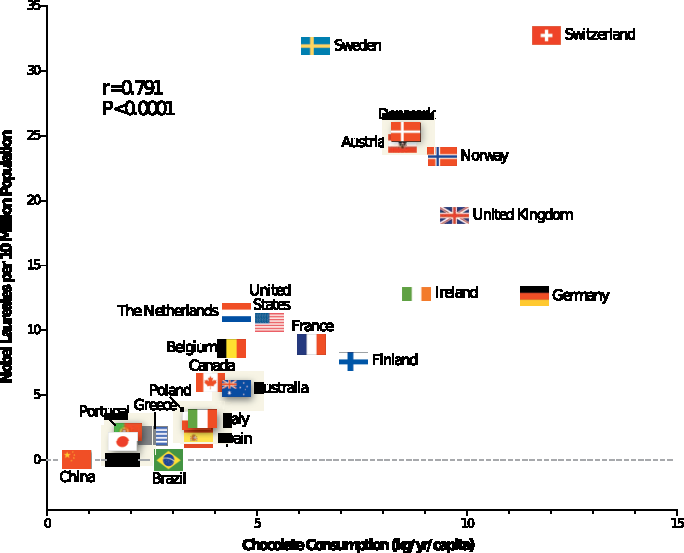
\includegraphics[width=\linewidth]{figures/chocolate-nobel}
  \caption{\label{fig:chocolate-nobel}
    From \parencite{messerli2012}.
    The figure shows a strong correlation between chocolate consumption
    in a country and number of Nobel prizes awarded to its citizens.
  }
\end{marginfigure}
A more scientific example is the unmistakeable correlation
shown in Figure~\ref{fig:chocolate-nobel}
between per-capita chocolate consumption
and number of Nobel laureates in a country.
Although the correlation is sound,
you should think twice before going into a chocolate diet
with the hope of winning a Nobel prize.

Another issue is that statistical dependence (correlation)
does not indicate the direction of the causation.
For example,
for a bystander observing a fire,
it may seem like `as more fire trucks arrive, the fire gets worse',
but the direction of causation is probably the other way around.
So although,
we won't be doing any analysis of causation,
you've been warned for this common error
(see also the cartoon in Figure~\ref{fig:xkcd-correlation}).
\begin{figure}
  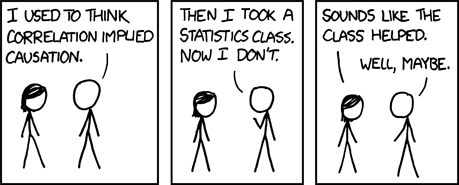
\includegraphics[width=\linewidth]{figures/xkcd-correlation}
  \caption{\url{http://xkcd.com/552/}}\label{fig:xkcd-correlation}%
\end{figure}

% TODO: multi-variate Gaussian?


\section{Where do the probabilities come from?}

So far,
we treated probabilities as numbers (between 0 and 1, inclusive)
and did not say much about where do they come from.
The question of what exactly a probability is a difficult one, 
and there have been (rival) alternative views on it.
Two well-known views,
we will encounter often is \emph{frequentist} (classical)
and \emph{Bayesian} (probabilistic) approaches.
Although both share all the aspects of probability theory we discussed above,
the interpretations of probability in these views differ,
and often lead to different methods for estimating probabilities.
This section is an informal, rather `philosophical', note on this difference.
We will frequently return to it later in this course.

In frequentist view,
the notion of probability is related to long-run relative frequency.
That is,
probability of an event is relative frequency of its occurrence.
For example,
if we are interested in probability of a particular word,
we can find it's relative frequency on a large corpus.
That is,
the number of times the word we are interested in appears in the corpus
divided by the number of words in the corpus.
Frequency-based probabilities leads to the estimation method called
\emph{maximum likelihood estimation} (MLE) we will discuss later.
% TODO: when/where?
The MLE is prevalent in statistics and machine learning.
As we will discuss in many places, however,
MLE \emph{overfits} the data it uses for the estimation,
the findings may not be general enough to be useful
outside the data used for estimation.
There are some modifications to MLE,
that makes it more resistant to overfitting.

In frequentist view of probability,
not every statement can be assigned to a probability value.
Some quantities we are often interested are fixed,
hence there is no notion of repeated experiments,
and hence, no probability value.
For example,
we can assign a probability value to
whether the next sentence in a speech (or in a book) will be
\num{10} words long.
Because this is a repeatable experiment.
However,
we cannot assign a probability value to average number of words
in a sentence in English (to simplify, say, in all written documents so far).
Even though we do not know this quantity,
there is a single number expressing it.
Hence, in frequentist view we cannot talk about,
the probability of average sentence length being \num{10}.
This seemingly `philosophical' standpoint has a very big impact
on how results are evaluated in experimental studies,
and hence, on the current scientific enterprise.

Intuitively,
frequency of an event and its probability is strongly related.
However,
our everyday notion of probability does
not necessarily involve repetitive experiments.
If you were given a fair coin,
you would not need a large number of experiments to conclude
that the probability of heads (or tails) is \num[round-precision=1]{0.5}.
On the practical side,
some events do not occur frequently enough to be estimated reliably.
As we will discuss at length in Chapter~\ref{chap:ngrams},
most objects of interest in NLP, such as words,
are particularly bad at showing up in where we look for them (in corpora).

The Bayesian notion of probability is based on (subjective)
`degree of belief',
matching more closely to our everyday notion of probability.
In this view,
probabilities are degrees of belief,
and updated `rationally',
with the data at hand based on rules of probability theory,
in particular based on the Bayes' formula we discussed in Section~\ref{sec:prob-bayes}.
Now that,
we consider probabilities as degrees of beliefs,
we can make probabilistic statements on things we are not allowed
in case of frequentist tradition.
For example,
we can easily talk about
the probability of average sentence length being \num{10},%
\footnote{Or, maybe between \num{9.5} and \num{10.5},
  since probabilities for single values is \num{0}
  for continuous random variables.}
and we can update this probability
(in fact the whole probability distribution) with the data we observe.
One particular benefit of the Bayesian estimation is that
we do not need anything other than probability theory for estimation.

A common criticism for Bayesian estimation is is that one needs to choose
a (subjective) prior probability (distribution)
before starting the data-driven estimation.
The word `subjective' does not sound like a good idea for science.
As a result,
Bayesian methods are often criticized for not being `objective'.
However, 
the prior information does not necessarily involve `personal' beliefs.
For example,
in our example with average number of words in a sentence,
there is nothing wrong to start with the presupposition that
the average number of sentences cannot be a negative number.
Further,
it is hardly a wrong assertion to assume that very large numbers,
e.g., \num{1000}, are very unlikely
(especially considering we are estimating \emph{average} sentence length).
There are many other forms of prior assumptions that are perfectly justified,
based on the knowledge accumulated in the field%
---often based on data from earlier studies.
Although making truly subjective decisions is not desirable
while interpreting experimental results in science,
if we shift our interest towards engineering rather than science,
the use of prior information (subjective or otherwise) is not
an issue at all.
There is nothing wrong with using a subjective method,
as long as it performs well for the task at hand.

A practical note on difference between the two estimation methods is
about the computational power required.
Bayesian estimation typically requires more computation power.
This difference is becoming less important
with the increasing power offered by developments in computer hardware
and approximate estimation techniques being developed.
However, it is still an important factor in many problems.

The debate is old and far from being settled yet.
In this course,
we do not take sides in this debate.
We introduce methods
that stem from both approaches for estimating probabilities.
The aim of this section is to inform the reader
about these different approaches
since they have important consequences for most of the methods we discuss.

% \section*{Where to go from here}
% 
% \textcite{grinstead2012} - online.
% 
% \textcite{mackay2003}
% 
% \textcite{jaynes2007}

\chapter{\label{chap:information-theory}Information theory}

The field of information theory is concerned with measurement, storage
and transmission of information.
I has its roots in communication theory,
but applications in many different fields including machine learning
and natural language processing.
In this chapter,
we will briefly introduce some of the main ideas,
and discuss a few important information theoretic measures
that will be used in the rest of the course.

\section{The noisy channel model}

A basic motivation in information theory is communication over 
a noisy channel.
In a \emph{noisy channel model},
as the one depicted in Figure~\ref{fig:noisy-channel},
the sender encodes the given message,
and sends it through the channel,
but the receiver receives a possibly corrupted version of the coded message.
\begin{marginfigure}
  \tikzsetnextfilename{noisy-channel}
  \begin{tikzpicture}
    \node (in) {a};
    \node[draw,thick,right=3mm of in, minimum height=4ex] (enc) {encoder};
    \node[draw,thick,right=15mm of enc, minimum height=4ex] (dec) {decoder};
    \node[right=3mm of dec] (out) {a};
    \node[below=0.5mm of enc,xshift=2em,font=\small]
      {100\textcolor{red}{0}0010};
    \node[below=0.5mm of dec,xshift=-2em,font=\small]
      {100\textcolor{red}{1}0010};
    \draw[thick,->] (in) -- (enc);
    \draw[thick,->] (dec) -- (out);
    \draw[thick,decorate, decoration={snake,post length=1mm},->]
      (enc) -- (dec)
      node[midway, above,yshift=2mm,font=\small,text width=1cm,align=center]
        {noisy\\channel};
  \end{tikzpicture}
  \caption{\label{fig:noisy-channel}%
    Schematic description of the noisy-channel model.
    The encoder codes the message and sends through a noisy channel
    to the decoder.
    The encoded message may possibly be corrupted during the transmission.
    The decoder's task is to reconstruct the original message,
    despite the potential noise introduced.
  }
\end{marginfigure}
The task of the decoder is to recover the original message,
even if there are some errors introduced in the noisy channel.
There are two competing objectives within the noisy channel model.
First, we want to use codes that use of the \emph{channel capacity}
as \emph{efficient}ly as possible.
We want coding schemes that result in short coded messages,
to transmit or store.
This is where the strong connection between the information theory 
and compression comes into the picture.
Second,
we want to be able to detect and correct the errors introduced by the noisy channel.
An obvious way to detect and correct errors is 
to send multiple copies of the code.
As we introduce more redundant copies,
it is more likely to recover the original message.
However,
replication also wastes the bandwidth of the channel.
Coding information efficiently,
while allowing error detection and error correction is fundamental
topics in information theory.
The example code in Figure~\ref{fig:noisy-channel},
is simply the ASCII code followed by an odd parity bit,
which means the last bit is set to \num{1} if the number of \num{1}s
in the code is an odd number,
otherwise,
the last bit is set to \num{0}.
Note that with the given code at hand,
the decoder can detect the error.%
\footnote{Can the decoder correct the error in Figure~\ref{fig:noisy-channel}?}
Here, we will not discuss error-correcting codes,
neither most of the other fascinating topics in information theory.
Interested readers are referred to the textbooks on information theory,
such as \textcite{mackay2003}.

Clearly, the noisy channel model is useful in the study of computer networks.
However, it has many other uses.
Note that the channel does not have to be a network connection.
For example,
the model fits equally well to storing data to a permanent storage.
Permanent storage systems (e.g., hard disks) are fairly accurate,
however, they are not error free.
As a result,
error resilience and efficiency is a concern here too.
The encoder encodes the information,
and sends it to the disk,
the decoder reads code (possibly after a long time) from the disk and
has to make sure that the information it decodes was not corrupted.

Beyond those obvious extensions,
the noisy channel model found its use in many other applications.
For an example close to home,
we often model \emph{speech recognition} with a noisy channel model.
The information here is a linguistic message,
e.g., a sentence.
The speaker codes this information as an acoustic signal,
and the recognizer's task is to decode the sentence
from the acoustic signal (code).
Another common use for the noisy channel model in NLP is
in machine translation, which we will return later.
We will not further discuss
the applications of the noisy channel model here.
However,
we introduce some of the concepts, particularly some measures,
that have very frequent uses in machine learning and NLP.

\section{Entropy and information}

In information theory,
\emph{entropy} is a measure of uncertainty.
The measure is analogous to `physical' entropy measure
in statistical thermodynamics,
but measures the uncertainty of
an information system rather than a physical system.
In ambiguous contexts, it is also called \emph{information entropy} or 
\emph{Shannon entropy} after Claude Shannon,
the inventor of the measure and the founder of the field.
Entropy and information are tightly connected concepts.
More concretely,
information in a message
(e.g., in the noisy channel model described above)
is the reduction of entropy after receiving the message.

Before introducing entropy properly,
we will first introduce a related measure \emph{surprisal},
which is also called \emph{self information}
or \emph{information content}.
The information theoretic measure of surprisal of an event $x$ is defined as
\begin{equation}\label{eq:surprisal}
  log \frac{1}{P(x)} = - log P(x) .
\end{equation}
If the probability of the event is \num{1}
(event occurs with certainty)
the surprisal will be \num{0}.
For events with decreasing probabilities,
we will get higher values for surprisal.
The value of surprisal will approach to $\infty$
while the probability of the event approaches to \num{0}.

The base of the logarithm in Equation~\ref{eq:surprisal}
is not very important,
since the logarithms in a different base can be obtained
by multiplication with a constant
(with a linear transformation).
Most common choices include base \num{2} logarithms,
which results in surprisal (or information) measured in \emph{bit}s.
If we use natural logarithm (with base $e$, Euler's number),
than the unit is called \emph{nat}.
In this course we will always use base-\num{2} logarithms,
and measure the information in bits.

The same quantity having names `surprisal' and `self information'
may not sound right at first sight.
The intuition here is that
we learn more from low-probability events.
Low probability events are surprising,
but also have more information content.
There is nothing surprising with
a weather report that tells it will rain in a very rainy country.
It also does not have much information content,
we can already predict it.
But if it predicts a sunny day in the middle of a rainy season,
then it is surprising as well as news-worthy,
it contains more information.

% The inverse relationship between surprisal and probability is intuitive.
% You may wonder, however, the reason for taking the logarithm.
% The main reason seems to be it is more convenient.
% We will try to get the intuition about logarithms with an example.
% Let's assume that we have a language with four letters,
% where occurrence of each letter has probability of \num{1/4},
% that is 
% 
% or information content of a state.
% High entropy means high unpredictability,
% hence high information content.
% If the outcome of a particular random variable is deterministic,
% then there is no uncertainty.
% Hence, the entropy is \num{0}.

Entropy of a system is the average surprisal.
We define entropy, $H$, of a random variable $X$ as
\begin{equation}\label{eq:entropy}
  H(X) = - \sum_{x \in X} P(x) log P(x)
\end{equation}
where, $x$ ranges over all values of $X$.
The above definition is for discrete variables,
which is much more common in NLP.
The notion of entropy can be extended to continuous random variables,
by replacing the sum with an integral
and $P(x)$ with the appropriate probability density function.
The resulting definition (for continuous random variables)
is called \emph{differential entropy}.

To get a sense of what entropy does,
consider the `guess the number' game,
where the first player picks a number between \num{1} and a larger number $M$,
(say 32),
and the task of the second player is to guess the number.
After every guess,
the first player tells whether the guess was
larger or smaller than the number he/she picked.
Assuming the first player picks the number completely randomly
(samples from the uniform distribution),
and if the second player follows the optimum strategy (binary search),
the first player will need to make $\log_{2} M$ guesses at most.%
\sidenote{What is the best strategy,
  if the number picked randomly,
  but follows a known non-uniform distribution?
}
Which is exactly what you will find if you use Equation~\ref{eq:entropy},
to calculate the entropy of this system.
For $M = 32$, 
\[
  H = - \sum_{1 \le x \le 32} \frac{1}{32} \log_{2} \frac{1}{32}
  = - 32 \frac{1}{32} \log_{2} \frac{1}{32} = - \log_{2} \frac{1}{32}
  = 5 .
\]
Note that since the numbers are equally likely,
probabilities for each number is the same ($1/32$).
As a result,
at the beginning we have \num{5} bits of entropy.
You should also see that we reduce the entropy by \num{1} bit for every guess
(unless we guess the correct number).
Hence, information we gain with every guess is \num{1} bit.

It is important to realize that
the entropy, or the information,
increase or decrease proportional to the logarithm of the states (the numbers).
If we double the range of numbers to pick from,
the entropy will not double, but only increase with one bit.
This logarithmic relationship is convenient,
since states of many systems we are interested in grow exponentially.

\begin{margintable}
  \caption{\label{tbl:binary-code-example}
    Example binary coding of an eight letter alphabet.
  }
  \begin{center}
    \begin{tabular}{lS[minimum-integer-digits=3]}
      \toprule
      letter & {code} \\
      \midrule
      a & 000 \\
      b & 001 \\
      c & 010 \\
      d & 011 \\
      e & 100 \\
      f & 101 \\
      g & 110 \\
      h & 111 \\
      \bottomrule
    \end{tabular}
  \end{center}
\end{margintable}
To get a sense of why logarithm is a good idea,
consider we want to code a \num{8}-letter alphabet on a binary medium
(or want to send over a binary channel).
We can use as many bits as the number of letters
(setting one of the bits to \num{1}, and the rest to \num{0},
similar to the one-hot representation discussed in Section~\ref{desc:one-hot}),
but this is wasteful.
The optimum coding would not require \num{8} bits.
We can easily represent \num{8} letters letters with \num{3} bits,
which turns out to be exaclty $\log_{2} 8$.
An example coding of \num{8}-letter alphabet is shown
in Table~\ref{tbl:binary-code-example}.
Note that if we double the letters,
we would not need to double the number of bits used,
all we need to do is add one more bit.
Hence,
the number of bits needed to represent $M$ letters is $log_{2} M$.
This is optimum if the letters we want to transmit are distributed uniformly.
We will soon see that we can do better,
if we have more structure in the distribution of the letters.


\begin{marginfigure}
  \tikzsetnextfilename{bernoulli-entropy}
  \begin{tikzpicture}[
  ]

      \begin{axis}[axis lines=left,
          enlarge x limits=true,
          enlarge y limits=upper,
          samples=50,
          width=1.1\linewidth,
          xlabel={$P(X=1)$},
          ylabel={$H(X)$},
          ylabel style={at={(rel axis cs:0,1)}, anchor=west,rotate=-90}
      ]
          \addplot[smooth, thick, blue, domain=0:1]
            {- x * (ln(x)/ln(2)) - (1-x) * (ln(1-x)/ln(2))};
      \end{axis}
  \end{tikzpicture}
  \caption{\label{fig:bernoulli-entropy}%
    Entropy of Bernoulli random variables (in bits)
    as a function of the parameter $p$. 
  }
\end{marginfigure}
For simplicity,
we assumed uniform distribution in the discussion/demonstration above.
What if the distribution of the random variable is not uniform?
To answer this question,
consider a Bernoulli trial, for example,
a coin-toss experiment or 
picking letters from a two-letter alphabet like Morse code.
If the letters were equally probable as in our earlier example,
the entropy would be,
\[
%  - \left(P(\mathbf{-}) \log P(\mathbf{-}) 
%      + P(\mathbf{\cdot}) \log (\mathbf{\cdot})\right)
  H = - \left(0.5 \times \log_{2} 0.5 + 0.5 \times \log_{2} 0.5 \right)
  = - \log_{2} 0.5 = 1.
\]
So, the entropy of a Bernoulli random variable with equal probabilities ($p = 0.5$),
such as outcome of a fair coin toss, is \num{1} bit.
We can also calculate the entropy with non-equal probability values.
For example, entropy of a Bernoulli random variable with $p=0.8$,
\[
%  - \left(P(\mathbf{-}) \log P(\mathbf{-}) 
%      + P(\mathbf{\cdot}) \log (\mathbf{\cdot})\right)
  H = - \left(0.8 \times \log_{2} 0.8 + 0.2 \times \log_{2} 0.2 \right)
  = \num{0.7219281} .
\]
Note that the entropy reduced from 1 bit to \num{0.7219281} bits.
This should all be intuitive,
since knowing that some of the outcomes are more likely than others reduces
the average surprisal.
If we do the above calculations for the parameter of Bernoulli distribution
$p$ in range $[0, 1]$,
we get the graph in Figure~\ref{fig:bernoulli-entropy}.
If the outcome of the variable is certain with $p = 1$ or $p = 0$,
then the entropy is \num{0},
and the entropy peaks at \num[round-precision=1]{0.5},
with a value of \num{1} bit,
where the uncertainty is at its maximum.

In general, uniform distribution is the distribution
with the maximum entropy
for distributions with the same support
(the set of values/events the distribution is defined on).
If the number of outcomes increase,
the uncertainty and the entropy will increase.
And, as the distribution diverges from the uniform distribution
by assigning higher probabilities to a small set of events,
the entropy will decrease.
Figure~\ref{fig:entropy-demo} demonstrates these two factors
with the categorical distribution.

\begin{figure}
    \tikzset{external/export next=false}
    %\tikzsetnextfilename{entropy-viz1}
    \begin{tikzpicture}[x=1mm,y=1mm]
      \newcounter{x}
      \newcounter{y}
      \def\xstep{22}
      \def\r{8mm}
      \draw[fill=blue!20] (\thex,\they) circle[radius=\r];

      \addtocounter{x}{\xstep}
      \filldraw[fill=green!20!white, draw=green!50!black]
          (\thex,0) ++(0:\r) arc[start angle=0, end angle=180, radius=\r] -- cycle;
      \filldraw[fill=blue!20!white, draw=green!50!black]
          (\thex,0) ++(180:\r) arc[start angle=180, end angle=360, radius=\r] -- cycle;

      \addtocounter{x}{\xstep}
      \filldraw[fill=green!20!white, draw=green!50!black]
          (\thex,0) ++(0:\r) arc[start angle=0, end angle=90, radius=\r] -- (\thex,0) -- cycle;
      \filldraw[fill=blue!20!white, draw=green!50!black]
          (\thex,0) ++(90:\r) arc[start angle=90, end angle=180, radius=\r] -- (\thex,0) --cycle;
      \filldraw[fill=red!20!white, draw=green!50!black]
          (\thex,0) ++(180:\r) arc[start angle=180, end angle=270, radius=\r] -- (\thex,0) --cycle;
      \filldraw[fill=gray!20!white, draw=green!50!black]
          (\thex,0) ++(270:\r) arc[start angle=270, end angle=360, radius=\r] -- (\thex,0) --cycle;

      \addtocounter{x}{\xstep}
      \filldraw[fill=green!20!white, draw=green!50!black]
          (\thex,\they) ++(0:\r) arc[start angle=0, end angle=60, radius=\r] -- (\thex,\they) -- cycle;
      \filldraw[fill=blue!20!white, draw=green!50!black]
          (\thex,\they) ++(60:\r) arc[start angle=60, end angle=120, radius=\r] -- (\thex,\they) --cycle;
      \filldraw[fill=red!20!white, draw=green!50!black]
          (\thex,\they) ++(120:\r) arc[start angle=120, end angle=280, radius=\r] -- (\thex,\they) --cycle;
      \filldraw[fill=gray!20!white, draw=green!50!black]
          (\thex,\they) ++(180:\r) arc[start angle=180, end angle=360, radius=\r] -- (\thex,\they) --cycle;

      \addtocounter{x}{\xstep}
      \filldraw[fill=green!20!white, draw=green!50!black]
          (\thex,\they) ++(0:\r) arc[start angle=0, end angle=30, radius=\r] -- (\thex,\they) -- cycle;
      \filldraw[fill=blue!20!white, draw=green!50!black]
          (\thex,\they) ++(30:\r) arc[start angle=30, end angle=60, radius=\r] -- (\thex,\they) --cycle;
      \filldraw[fill=red!20!white, draw=green!50!black]
          (\thex,\they) ++(60:\r) arc[start angle=60, end angle=90, radius=\r] -- (\thex,\they) --cycle;
      \filldraw[fill=gray!20!white, draw=green!50!black]
          (\thex,\they) ++(90:\r) arc[start angle=90, end angle=360, radius=\r] -- (\thex,\they) --cycle;


      \foreach[count=\i, evaluate=\i as \x using int((\i-1)*\xstep)] \v in {0,1,2,1.79,1.06}{%
        \node[anchor=north] at (\x,-10) {$H = \v$};
      }
    \end{tikzpicture}
    \caption{
      Demonstration of entropy values (in bits)
      with the categorical distribution.
      First three circles from the left represent
      uniform categorical distributions with increasing number of categories.
      Increasing possible outcomes increase the uncertainty, hence the entropy.
      Last three circles demonstrate categorical distributions with equal
      number of possible outcomes.
      As the distribution diverge from the uniform distribution,
      the uncertainty and entropy is reduced.
    }\label{fig:entropy-demo}%
\end{figure}

By now,
you should be able to calculate the entropy of a categorical distribution
over \num{8} symbols,
just like the letters in Table~\ref{tbl:binary-code-example}.
Given that these letters are distributed uniformly
(each having probability of $1/8$),
the entropy of the distribution is \num{3} bits,
which corresponds to how many bits we need for optimally coding the alphabet.
We noted that we can do better if the distribution was not uniform.
Let us assume that,
the letter `a' occurs with probability $1/2$,
the letter `b' occurs with probability $1/4$,
the letter `c' occurs with probability $1/8$,
the letter `d' occurs with probability $1/16$,
and the other letters occur with probability $1/64$.
Now, using trhee bits for all comibinations is just wasteful.
We can do much better with the codes on Table~\ref{tbl:huffman-code-example}.
The type of coding example here is called \emph{Huffmann} coding.
Although the number of bits are variable,
we can unabiguously determine each code with its prefix.
One can easily show that this coding requires less storage or channel bandwidth
on average.
In fact,
this corresponds to the entropy of the distribution,
which is \num{2} bits:
we save \num{1} bit on average.
This is exactly another way to interpret entropy,
it is the average code-length for the best achievable code
for a given distribution.
In other words,
entropy gives us the upper bound on
an optimal encoder (in terms of efficient channel utilization)
in a noisy channel model (Figure~\ref{fig:noisy-channel}).
\begin{margintable}
  \caption{\label{tbl:huffman-code-example}
    Example Huffman coding of an eight letter alphabet.
  }
  \begin{center}
    \begin{tabular}{lrl}
      \toprule
      letter & prob &{code} \\
      \midrule
      a & $1/2$&  \num{0} \\
      b & $1/4$&  \num{10} \\
      c & $1/8$&  \num{110} \\
      d & $1/16$& \num{1110} \\
      e & $1/64$& \num{111100} \\
      f & $1/64$& \num{111101} \\
      g & $1/64$& \num{111110} \\
      h & $1/64$& \num{111111} \\
      \bottomrule
    \end{tabular}
  \end{center}
\end{margintable}


% \begin{margintable}
%   \caption{\label{tbl:cond-prob-table}%
%     Conditional probabilities of $P(\text{letter}\:\vert\:\text{dialect})$.
%   }
%   \begin{center}
%     \setlength{\tabcolsep}{4pt}
%     \begin{tabular}{lS[round-precision=3]S[round-precision=3]S[round-precision=3]}
%       \toprule
%       let. & {east} & {north} & {south} \\
%       \midrule
%       a & 0.2829786& 0.0326985& 0.283765\\
%       b & 0.0413973& 0.0624915& 0.009443\\
%       c & 0.0363760& 0.0465435& 0.116444\\
%       d & 0.0892564& 0.0738920& 0.068607\\
%       e & 0.2458984& 0.4862595& 0.165408\\
%       f & 0.0241540& 0.0131360& 0.067122\\
%       g & 0.0720066& 0.0647505& 0.000000\\
%       h & 0.2079327& 0.2202285& 0.289211\\
%       \bottomrule
%     \end{tabular}
%   \end{center}
% \end{margintable}
\begin{margintable}
  \caption{\label{tbl:marginal-prob-table2}%
    Joint probability table for letters and dialects
    with marginal probabilities.
    $P(D)$ is the (marginal) probability of dialects,
    and $P(L)$ is the probability of letters in the corpus.
    This is the same as Table~\ref{tbl:marginal-prob-table},
    repeated here for convenience.
  }
  \begin{center}
    \setlength{\tabcolsep}{4pt}
    \begin{tabular}{lS[round-precision=2]S[round-precision=2]S[round-precision=2]|S[round-precision=2]}
      \toprule
      let. & {east} & {north} & {south} & {$P(L)$} \\
      \midrule
      a & 0.1980850&0.0065397&0.0283765 & 0.2330012\\
      b & 0.0289781&0.0124983&0.0009443 & 0.0424207\\
      c & 0.0254632&0.0093087&0.0116444 & 0.0464163\\
      d & 0.0624795&0.0147784&0.0068607 & 0.0841186\\
      e & 0.1721289&0.0972519&0.0165408 & 0.2859216\\
      f & 0.0169078&0.0026272&0.0067122 & 0.0262472\\
      g & 0.0504046&0.0129501&0.0       & 0.0633547\\
      h & 0.1455529&0.0440457&0.0289211 & 0.2185197\\
      \midrule
      $P(D)$  & 0.7&0.2&0.1 & 1.0\\
      \bottomrule
    \end{tabular}
  \end{center}
\end{margintable}
To give a more concrete example,
we re-introduce our dialects with eight letters from Chapter~\ref{chap:prob}.
Table~\ref{tbl:marginal-prob-table2} lists the joint probabilities of 
letters and dialects (east, north and south),
as well as marginal probabilities.
From this table,
we can easily calculate the entropy of the distributions of letters for the 
complete language,
and the entropy of the letter distribution for each dialect.
Now you should take a moment and try to phrase
what high or low entropy means for letters or dialects.
For the sake of making things more concrete,
we will calculate the entropy of dialect distribution in our document set.
The entropy of letter distribution over dialects
\[
  H(d) = -\left(0.7 \times log_{2} 0.7 + 0.2 \times log_{2} 0.2 + 0.1 \times log_{2} 0.1\right)
       = \num{1.15678}
\]
is lower than a uniform distribution of letters over the dialects
which is \num{1.584963}.
In other words,
by knowing $P(D)$, we gain \num{0.428183} bits of information,
in comparison to a setting where the dialects were equally represented
in the data.
The distribution over individual letters is more interesting,
you are encouraged to calculate the entropy of letters ($P(L)$)
and compare it with a uniform distribution.
Note that if you want to calculate entropy of letters within each dilaect,
you need conditional probabilities, e.g., $P(L\given{}D=\text{east})$,
for calculating letter-entropy values of individual dialects.
%\todo{exercise}

\begin{tcolorbox}
  Note that entropy is about complete probability distributions,
  while surprisal is about probabilities of individual events.
\end{tcolorbox}

\section{Mutual Information and conditional entropy}

Another very important quantity from information theory used 
widely in computational and corpus linguistics is \emph{mutual information}.
Mutual information measures
the amount of information obtained (reduced entropy) about a random variable,
by knowledge of another random variable.
Mutual information is a measure of dependence between two variables.
If the variables are dependent (provide information about each other),
then the mutual information will be high.
If the variables are independent the mutual information will be \num{0}.

As we did with introduction to entropy,
we will first introduce another relevant measure,
\emph{pointwise mutual information} (PMI),
which measures the (in)dependence of two events.
The PMI value for two events
$X = x$ (or simply $x$) and $Y = y$ (or $y$) is calculated by
\begin{equation}\label{eq:pmi}
  \text{PMI}(x, y) = \log \frac{P(x,y)}{P(x)P(y)}
\end{equation}
A quick study of the formula indicates
that pointwise mutual information is high
if the joint probability of the two events involved is high.
However,
since the high-probability events can cooccur by chance frequently,
the denominator of the term in Equation~\ref{eq:pmi} includes
(marginal) probabilities of both events.
Hence, it discounts the by-chance cooccurrences of the events
due to high marginal probability.
Remember that the joint probability of two independent events is
the product of their probabilities ($P(x,y) = P(x) P(y)$,
for independent events $x$ and $y$).
As a result,
the division within the logarithm in Equation~\ref{eq:pmi} will result in \num{1},
and PMI will be \num{0}, for independent events.
If two events are highly positively associated (they occur together),
then PMI will be positive,
and if events are highly negatively associated
(one does not occur if the other event occurs),
then the PMI value will be negative.

Just for the sake of example,
we will calculate the PMI of letter `e' occurring in the `east' dialect
in the distribution presented in Table~\ref{tbl:marginal-prob-table2}.
\[
  \text{PMI}(\text{east},\text{e})
    = log \frac{P(\text{east}, \text{e})}{P(\text{east})P(\text{e})}
    = log \frac{\num{0.1721289}}{\num{0.7}\times \num{0.2859216}}
    = \num{-0.2175571}
\]
Despite the fact that the joint probability of the two events is rather high,
we find a negative association between them%
---in `e', in fact, occurs less than chance in the eastern dialect.

One of the most common uses of PMI is to find \emph{collocations},
groups of words that occur frequently together.
Using PMI,
it is likely to find linguistically plausible collocations like,
`corpus linguistics',
even though it is much less likely than non-interesting frequent bigrams like `that the'.

The \emph{mutual information} (MI) of two random variables
is a measure of dependence of the variables.
Mutual information is the expected value of (average) PMI.
The mutual information of two discrete random variables $X$ and $Y$ is
\begin{equation}\label{eq:mi}
  \text{MI}(X, Y) 
    = \sum_{x\in X} \sum_{y\in Y} P(x,y) \log \frac{P(x,y)}{P(x)P(y)} .
\end{equation}

Similar to PMI,
a positive MI value indicates a positive association between
the random variables,
zero indicates independence (no association),
and negative values indicate negative association.
Like \emph{correlation} (Section~\ref{sec:correlation}),
mutual information measures dependence between two random variables.
However, unlike correlation, it is not limited to linear dependence.

Mutual information is related to entropy
through a measure known as \emph{conditional entropy}.
We note the conditional entropy of a random variable $X$ given
another random variable $Y$ takes the value $y$ as $H(X\given{}Y=y)$.
Intuitively,
if the event $Y=y$ gives information about the random variable $X$,
we expect low conditional entropy.
The conditional entropy of $X$ given $Y$,
noted $H(X\given{}Y)$,
is the average entropy of $X$ given $Y$.
The conditional entropy of $X$ given $Y$ can be calculated by
\begin{equation}\label{eq:conditional-entropy}
  \begin{aligned}
    H(X\given{}Y) &= & &\sum_{y\in Y} P(y) H(X\given{}Y=y)\\
                  &= &- & \sum_{x\in X, y\in Y} P(x,y) \log P(x\given{}y)
  \text{.\footnotemark}\\
  \end{aligned}
\end{equation}%
\footnotetext{You are recommended to derive this equation.
 Meanwhile, you may also want to show that
 \[ 
    H(X\given{}Y) = \sum_{x\in X, y\in Y} P(x,y) \log \frac{P(y)}{P(x,y)}
 \]
 is also correct.
}

The conditional entropy has also a straightforward interpretation.
The conditional entropy $H(X\given{}Y)$ equals to
the entropy of the variable $X$ ($H(X)$),
if the variables are independent.
As the dependence between variables increase,
the conditional entropy will decrease.


\begin{marginfigure}
  \tikzsetnextfilename{entropy-mi-relation}
  \begin{tikzpicture}
%    \draw[help lines] (0,0) grid (5,5);
    \node[draw,circle,minimum size=3.5cm,inner sep=0pt,fill=blue,opacity=0.2]
      at (2,2) {};
    \node[draw,circle,minimum size=3.5cm,inner sep=0pt,fill=red,opacity=0.2]
      at (3,3) {};
    \node at (0.7,3.7) {$H(X)$};
    \node at (4.3,1.3) {$H(Y)$};
    
    \node at (1.3, 1.5) {$H(X\given{}Y)$};
    \node at (3.7, 3.5) {$H(Y\given{}X)$};

    \node at (2.5, 2.5) {$MI(X,Y)$};

    \node at (3.5, 0) {$H(X,Y)$};
  \end{tikzpicture}
  \caption{\label{fig:entropy-mi}%
    Relation between conditional entropy entropy and mutual information.
    The total shaded area is the joint entropy of two variables $H(X,Y)$.
  }
\end{marginfigure}

Note that entropy, conditional entropy, and mutual information are all related.
Figure~\ref{fig:entropy-mi} shows the relationship between these measures
schematically using a Venn diagram.
For example, we can see from the figure that $H(X,Y) = H(X) + H(Y) - MI(X,Y)$.
The total entropy associated with two random variables is reduced if the 
mutual information (dependence) between them is high.
If one of the variables ($Y$) completely determines the other ($Y$),
the conditional entropy ($H(X|Y)$) will be \num{0},
the joint entropy will be equal to the entropy of one one of the variables
($H(Y)$),
and mutual information will be equal to entropy of the other variable $H(X)$.
The mutual information is symmetric ($MI(X,Y) = MI(Y,X)$),
while conditional entropy is not ($H(X\given{}Y) \ne H(Y\given{}X)$). 
Also note that the relationships
between the information theoretic measures are additive,
while the relationship between the corresponding probabilities are multiplicative.

\section{Cross entropy}

\emph{Cross entropy} is another important concept from information theory
that has wide usage, particularly in machine learning.
Remember that entropy gives us the best achievable compression
given a distribution.
In many practical cases we do not know the true distribution of the data,
instead we use an approximate one.
If we do not use the true distribution,
inevitably, our code will be less optimum.
This means that we will get higher entropy.
If the true distribution is $P(x)$ and the its approximation is $\hat{P}(x)$,
the cross entropy is defined as
\begin{equation}
  H(P, \hat{P}) = - \sum_{x} P(x) log \hat{P}(x) .
\end{equation}
The hat-notation used here is used for estimated objects.
If $P$ was the true distribution,
we would note an estimation of it as $\hat{P}$.
Although this is most common context we will see cross entropy used,
the distribution $\hat{P}$ does not have to be an estimate of $P$.
Technically, the only requirement is
that the distribution should have the same support.
Note that the notation $H(X, Y)$ is also used for joint entropy,
but for joint entropy the arguments are random variables
noted like $X$ and $Y$,
and for cross entropy distribution functions
noted with letters like $P$ and $Q$.

The formula above makes sense if you think about it
in terms of the noisy channel model.
Remember that we are coding the data using $\hat{P}$,
hence the code length is determined by the approximate model.
However, the average is taken over the true distribution,
hence, we multiply by $P(x)$ not $\hat{P}(x)$.
Cross entropy is always larger than entropy.
Since we are using the wrong (approximate) distribution to code the data,
the code length will not be optimum.
As $\hat{P}$ gets closer to the $P$,
the cross entropy will approach the entropy of $P$.
Note that cross entropy is not symmetric ($H(P, Q) \ne H(Q, P)$).

A very common use of cross entropy is as a \emph{loss function}
in some machine learning methods.
In many machine learning methods,
training the model is equivalent to minimizing a loss function.
Hence,
as we minimize cross entropy of true distribution
that comes from the training data
and the approximate distribution the machine learning system produces,
we get closer to the true distribution of the answers we are seeking.
That way,
the output of the machine learning model becomes
more similar to the expected output.
We will see example uses of cross entropy later in this course.

\begin{margintable}
  \caption{\label{tbl:east-overall}%
    Probability distributions of letters in our hypothetical dialect data.
    $P(L\given{}D=\text{east})$ is the distribution of letters
    given the dialect is east dialect,
    $P(L)$ is the marginal distribution of letters (for all dialects).
  }
  \begin{center}
    \setlength{\tabcolsep}{4pt}
    \begin{tabular}{lS[round-precision=2]S[round-precision=2]}
      \toprule
      let. & {$P(L\given{}\text{east})$} & {$P(L)$} \\
      \midrule
      a & 0.2829786 & 0.2330012\\
      b & 0.0413973 & 0.0424207\\
      c & 0.0363760 & 0.0464163\\
      d & 0.0892564 & 0.0841186\\
      e & 0.2458984 & 0.2859216\\
      f & 0.0241540 & 0.0262472\\
      g & 0.0720066 & 0.0633547\\
      h & 0.2079327 & 0.2185197\\
      \bottomrule
    \end{tabular}
  \end{center}
\end{margintable}
For a concrete example,
we return to the hypothetical dialects with \num{8}-letter alphabets
in Table~\ref{tbl:marginal-prob-table2}.
Assume that we do not know the distribution of the letters
in the eastern dialect,
and we are using the total distribution
for coding (e.g., compressing) the data from the eastern dialect.
Both distributions are summarized in Table~\ref{tbl:east-overall}.
We simply calculate cross entropy by 
\[
  \begin{aligned}
    H\left(P(L\given{}\text{east}), P(L)\right) 
      = - \sum_{x\in \text{letters}} P(x\given{}\text{east}) \log_{2} P(x)
      = \num[round-precision=3]{2.577201} .
  \end{aligned}
\]
As expected,
this is larger than entropy of $P(L\given{}\text{east})$,
which is \num[round-precision=3]{2.562475} bits.

\section{Perplexity}

A measure related to entropy,
used often in computational linguistic literature,
is \emph{perplexity} (PP).
Perplexity is simply the exponentiated version of entropy.
If we measure entropy in bits, then the perplexity is
\begin{equation*}
  \text{PP}(X) = 2^{H(X)} .
\end{equation*}

Like entropy, perplexity measures uncertainty.
However, since it measures it in a different scale,
sometime it offers a more intuitive interpretation.
Its main use in NLP is evaluating language models,
which are conditional distributions on words given a history of earlier words.
In this context, the intuitive interpretation is
the average number of words expected after each word.

\section{Kullback--Leibler divergence}

\begin{marginfigure}
  \tikzsetnextfilename{kl-divergence-viz}
  \begin{tikzpicture}[
      declare function={%
        normpdf(\x,\m,\s) = exp(-(\x -\m)^2/(2*\s)^2) /%
                                (\s*(2*pi)^0.5);%
      }
  ]
      \begin{axis}[
          axis lines=middle,
          hide y axis,
          enlargelimits=true,
          samples=50,
          x=4mm,
          y=70mm,
          ymin=0,
          clip=false,
          x axis line style={<->}
      ]
          \addplot[smooth, thick, blue, domain=-6:6,name path=curve1]
            {normpdf(x,-0.5,1)};
          \addplot[smooth, thick, red, domain=-6:6,name path=curve2]
            {normpdf(x,0.5,1.2)};
          \addplot[draw=none, domain=-6:6,name path=xax] {0};
          \addplot[blue,opacity=0.2]
            fill between[of=curve1 and xax,soft clip={domain=-5:5}];
          \addplot[red,opacity=0.2]
            fill between[of=curve2 and xax,soft clip={domain=-5:5}];
          \node[blue] at (-4.2, 0.1) {$P$};
          \node[red] at (3.8, 0.1) {$Q$};
          \node (a) at (2, 0.15) {};
          \node (kpq) at (4, 0.3) {$D_{KL}(P\;\Vert\;Q)$};
          \draw[->] (a) --  (kpq);

          \node (b) at (-1.6, 0.18) {};
          \node (kqp) at (-4, 0.3) {$D_{KL}(Q\;\Vert\;P)$};
          \draw[->] (b) --  (kqp);
      \end{axis}
  \end{tikzpicture}
  \caption{\label{fig:kl-diverngence}%
    Visualization of KL divergences between two distributions.
    Note, however, this is a demonstration to show the asymmetry
    of measure, the areas indicated are not exactly what
    KL-divergence measures.
  }
\end{marginfigure}
Another important quantity we often see during this course is
\emph{Kullback-Leibler divergence} which is also known as
\emph{relative entropy}.
It is often abbreviated as \emph{KL divergence}.
Similar to cross entropy,
KL divergence is a about two probability distributions with the same support.
It measures the amount of information lost,
or extra bits of entropy,
while using a distribution $Q$ instead of using the true distribution $P$.
It is defined as,
\begin{equation}\label{eq:kl-divergence}
  D_{KL} (P\;\Vert\;Q) = - \sum_{x} P(x) \log \frac{P(x)}{Q(x)}.
\end{equation}
It is the average logarithmic difference
between distributions $P$ and $Q$,%
\footnote{%
  Remember that 
  \[
    \log \frac{a}{b} = \log(a) - \log(b) .
  \]
}
where average calculated according to $P$.
KL divergence is often used as a measure of difference
between two distributions.
However, it is not symmetric
(as a result, it is not a proper distance measure).
Figure~\ref{fig:kl-diverngence} visualizes the KL divergence
between two continuous distributions.
For continuous distributions,
as usual,
you can simply replace probability mass functions
with probability density functions, 
and summation with the integral in Equation~\ref{eq:kl-divergence}.

For a concrete example,
we will return to the question of using an approximate distribution,
the marginal letter distribution,
instead of one of the conditional distributions
in our letter distribution example in Table~\ref{tbl:east-overall}.
As in our cross entropy example,
assume that we do not know the distribution of the eastern dialect,
and approximating it with the marginal distribution.
If we do the calculation,
\[
  D_{KL} \left(P(L\given{}\text{east})\;\Vert\;P(L)\right) = - \sum_{x} P(x|\text{east}) \log \frac{P(x|east)}{P(x)}
  = \num[round-precision=3]{0.0147261}
\]
which is the amount of information we lose by using the marginal distribution
instead of the dialect-specific distribution in bits.

Conceptually,
you should already be expecting a link between 
the cross entropy and the KL divergence divergence.
Cross entropy measures the entropy of a distribution ($P$) under 
another distribution ($Q$),
while KL divergence measures the amount of additional entropy if one uses one distribution ($Q$) instead of another ($P$).
As a result,
\[
  H(P, Q) = H(P) + D_{KL}(P\;\Vert\;Q).
\]

You can easily verify this
with our running example of dialect letter distributions as well
(maybe with some rounding error).

% \section*{Where to go from here}
% 
% \textcite{mackay2003}
% 
% \textcite{pierce1980}
% 
% \textcite{stone2015}
% 
% \textcite{ghahramani2003}
% 
% \textcite{shannon1948}
% 
% \textcite{seife2007}
% 
% \section*{Exercises}
% 
% % \begin{question}
%   What is the name of the following measure?
%   \[
%     \log \frac{P(x\given{}y)}{P(x)}
%   \]
% \end{question}

% p = c(0.2829786, 0.0413973, 0.0363760, 0.0892564, 0.2458984, 0.0241540, 0.0720066, 0.2079327)
% q = c(0.2330012, 0.0424207, 0.0464163, 0.0841186, 0.2859216, 0.0262472, 0.0633547, 0.2185197)

%\chapter{\label{chap:inference}Statistical models:
  learning, estimation, inference and prediction}

% If we know that we have a fair coin,
% we can calculate the probability of obtaining
% a certain number of heads in a sequence of coin tosses
% using probability theory.
% What if, we do not know if the coin is fair or not?
% Can we \emph{infer} whether the coin is fair or not
% from a finite number of outcomes?
% Similarly,
% if we know the election results in a country,
% probability theory can tells us
% the probability of a randomly picked the voters
% having voted a particular political party.
% But what can we say about the election results,
% given we know which parties a limited number of voters will vote?
% In general,
% given a finite sample of data,
% we want to know, or infer,
% some properties of the data source (e.g., population)
% that the data comes from.
% These questions fall into the area of \emph{statistical inference}.

Modeling natural phenomena is one of the basic activities in science.
We build models of a natural phenomenon to gain a better insight
into the phenomenon being modeled,
and predict aspects that we do not know about it.
Models are used in many fields in science and engineering.
Just to name a few well-known examples,
we note Galilean model of solar system in astronomy;
Bohr model of atom in physics;
animal models in medicine that are used for studying human diseases
on non-human animals;
econometric models in economics;
the formal models of atmospheric conditions used for weather forecasts; 
scaled physical models of bridges, cars, and other objects
that are used frequently in design and engineering of these objects.

Whether they are abstract (mathematical) models,
or physical ones,
these models allow us to study the phenomenon being modeled
in a convenient way.
They allow us to test hypotheses and make \emph{inferences}
or \emph{predictions} that we cannot do directly
on the real object being studied.

In this lecture, we are interested in
\emph{statistical model}s
which constitute a very broad range of models used in many disciplines.
In a statistical model,
part of the phenomenon being modeled is subject to uncertainties.
As a result,
the data we collect or observe does not lead to fully deterministic model. 
Statistical models are the main subject of study
in statistics and machine learning,
and naturally, has a very important role in natural language processing.

Before this general introduction to statistical models,
we remind that ``all models are wrong, some are useful.''%
\autocite[p.~424]{box1986}
In any modeling effort,
one has to make simplifications or assumptions that do not match
with the object or the process being modeled.
However,
as long as we are aware of its shortcomings,
we can build useful models.

\section*{Where to go from here}

\textcite{wasserman2004}

\chapter{\label{chap:ml-basics}Machine learning basics}

Statistical methods,
particularly methods from machine learning,
has been the most successful solutions for many
applications dealing with natural languages.
The methods from machine learning dominates the filed
so much that many people consider NLP as a branch of machine learning.

Machine learning is about learning from data.
Instead of writing a specialized program based on expert knowledge
for solving a problem, we rely on generic `programs', or  models,
which learn from data.
As noted above, this has proven useful in many applications.
However, machine learning also offers us ways to 
analyze the data at hand and arrive at generalizations
that are sometimes impossible without use of these techniques.

This lecture introduces some of the basic ideas behind machine learning,
alongside linear regression,
a simple but fundamental model for learning from data.

\section{Machine learning: broad categorization of methods}

Machine learning methods are categorized
into a number of broad categories in the literature.
Most commonly, the methods are categorized
based on the amount of supervision they need.
On the one hand,
a \emph{supervised} method requires labeled data.
That is, every object we want to classify (e.g., a document) 
has to be annotated with target information  want to predict
(e.g., the author of the document) in the training data.
However, the aim of the method is
to make predictions outside its training set.
We want our models to generalize not memorize.
On the other hand,
an \emph{unsupervised} method does not require
any target label or information.
The aim is to use the differences and similarities
between the data points for finding useful patterns.
The methods that exploit both annotated data
(with target label/information) and unannotated data
are called \emph{semi-supervised}.
Another interesting class of methods
where success and failure is not associated with 
individual predictions but a collection of them
is called \emph{reinforcement learning}.

In this course we mostly focus on supervised methods,
but also cover some of the unsupervised methods
commonly used in the field.

\newthought{In supervised learning} the training data contains
what we want to predict.
The task of the system is, then,
to learn this predictions from the training data
in a way that it is useful for
making predictions for new, unseen instances.
An overall picture of supervised learning is provided
in Figure~\ref{fig:supervised-learning}.

\begin{figure}
%  \tikzset{external/export next=false}
  \tikzsetnextfilename{supervised-learning-diagram}
  \begin{tikzpicture}[node distance=8mm]
    \tikzset{mnode/.style={draw,
                           font=\small,
                           text width=width("predicted"),
                           minimum width=width("predicted"),
                           align=center,
                           minimum height=5ex,
                           inner sep=2pt,
                           rounded corners,
                           }
    }
    \node[mnode,fill=green!20] (train) {training data};
    \node[mnode,fill=green!20, right=of train] (feat) {features};
    \node[coordinate, below=of train] (dummy) {};
    \node[mnode,fill=green!20, below=of dummy] (label) {labels};
    \node[mnode,fill=green!20, below right=of feat] (ml) {ML algorithm};
    \node[mnode, right=of ml,fill=orange!50] (model) {ML model};
    \node[mnode,fill=blue!20, above=of model] (nfeat) {features};
    \node[mnode,fill=blue!20, above=of nfeat] (newd) {new data};
    \node[mnode,fill=blue!20, below=of model] (pred) {predicted label};

    {[on background layer]
      \node[mnode,fill=green!20] at ([xshift=-6pt,yshift=6pt]train) {};
      \node[mnode,fill=green!20] at ([xshift=-4pt,yshift=4pt]train) {};
      \node[mnode,fill=green!20] at ([xshift=-2pt,yshift=2pt]train) {};

      \node[mnode,fill=green!20] at ([xshift=-6pt,yshift=6pt]feat) {};
      \node[mnode,fill=green!20] at ([xshift=-4pt,yshift=4pt]feat) {};
      \node[mnode,fill=green!20] at ([xshift=-2pt,yshift=2pt]feat) {};

      \node[mnode,fill=green!20] at ([xshift=-6pt,yshift=6pt]label) {};
      \node[mnode,fill=green!20] at ([xshift=-4pt,yshift=4pt]label) {};
      \node[mnode,fill=green!20] at ([xshift=-2pt,yshift=2pt]label) {};

      \draw[blue!20,very thick,->]
        ([xshift=2mm]newd.north east) -- ([xshift=2mm]pred.south east)
        node[blue,midway, above,rotate=-90] {prediction};
      \draw[green!20,very thick,->]
        ([yshift=2mm]train.west |- model.north)
          -- ([yshift=2mm]model.north east)
        node[green,near start,below] {training};
    }

    \draw[thick,->] (train) -- (feat);
    \draw[thick,->] (feat) -- ([yshift=2pt]ml.west);
    \draw[thick,->] (label) -- ([yshift=-2pt]ml.west);
    \draw[thick,->] (ml) -- (model);

    \draw[thick,->] (newd) -- (nfeat);
    \draw[thick,->] (nfeat) -- (model);
    \draw[thick,->] (model) -- (pred);
  \end{tikzpicture}
  \caption{
    A picture of supervised learning.
  }\label{fig:supervised-learning}%
\end{figure}

During training, we need both our training data and
the associated predictions (indicated as `labels' in Figure~\ref{fig:supervised-learning}).
Typically, the objects we want to work with cannot be
used directly with a machine learning algorithm.
We need to first extract features that are useful for prediction
and can be represented in a form the machine learning algorithms can work with.
For example, to classify documents,
we may use the length of the documents,
or number of times a particular word occurs in the document as features.
The role of the machine learning algorithm is to find the best model
(among a family of models) based on the training set.
During prediction time,
we first extract the features from a new data instance the same way we did during training,
and predict the outcome using the model.
An important point that is worth repeating is
we want our model to perform well on the new data.%
\sidenote[][-1cm]{And, we will repeat this many times in this class.}

      \pgfplotstableread{
        X Y
        0.8 1.7
        2.1 5.0
        2.9 4.
        4.1 2.6
        4.9 3.6
        6.1 7.2
        6.9 6.1
        8.1 8.9
        8.9 8.4
      }\regtable

\begin{marginfigure}
%  \tikzset{external/export next=false}
  \tikzsetnextfilename{regression-example}
  \begin{tikzpicture}
    \begin{axis}[x=5mm, y=3mm,
                 ticklabel style={font=\tiny},
                 grid=major,
                 grid style={draw=gray!10},
                 major grid style={draw=gray!40},
%                 minor tick num=4,
                 xmin=0,
                 xlabel={$x$},
                 ylabel={$y$},
                 xlabel style={font=\tiny},
                 ylabel style={font=\tiny},
                 axis y line=left,
                 axis x line=bottom,
                 xlabel style={at={(rel axis cs:1,0)}, anchor=south east},
                 ylabel style={at={(rel axis cs:0,1)}, anchor=north west,rotate=-90},
                 ymin=0,
      ]

      \addplot[only marks, mark size=0.4mm,fill=blue] table {\regtable};
      \addplot [no marks, thick, red]
        table [y={create col/linear regression={y=Y}}] {\regtable};
      \addplot[no marks,thick,red,domain=0:9]
        {\pgfplotstableregressiona*x+\pgfplotstableregressionb};
      \draw[blue] (5.5,0) -- (5.5, \pgfplotstableregressiona*5.5+\pgfplotstableregressionb);
      \draw[blue] (5.5, \pgfplotstableregressiona*5.5+\pgfplotstableregressionb) -- (0, \pgfplotstableregressiona*5.5+\pgfplotstableregressionb);
      \node[inner sep=1pt,blue,anchor=south east,font=\tiny] at (5.5, 0) {$5.5$};
      \node[inner sep=1pt,blue,anchor=north west,font=\tiny] at (0, 5.7) {$5.7$};
    \end{axis}
  \end{tikzpicture}
  \caption{\label{fig:regression-example}
    A demonstration of simple linear regression.
  }
\end{marginfigure}
If a supervised machine learning model predicts a numeric value
it is called a \emph{regression} model.
A simple regression model predicting one numeric variable ($y$)
from a single numeric predictor ($x$) is demonstrated
in Figure~\ref{fig:regression-example}.
The small circles on the plot represent the pairs of $x$,$y$ values observed.
The red line is the model after observing this `training' data.
Once we have the model,
our predictions for the new data points will be based on this line.
The blue lines on the figure demonstrate the prediction of the model
for $x=5.5$, which turns out to be $5.7$ according to this model.

\begin{marginfigure}
%  \tikzset{external/export next=false}
  \tikzsetnextfilename{classification-example}
  \begin{tikzpicture}[x=5.5mm, y=4mm]
    \draw[->,thick] (0,0) -- (0,6.5);
    \draw[->,thick] (0,0) -- (7.5,0);
    \node[rotate=90] at (-0.5, 3) {$x_{2}$};
    \node at (4, -0.5) {$x_{1}$};
%    \draw[-,thick] (0.1,5.5) -- (6.5, 0.1);
    \node[green] at (3.4,3.4) {?};
    \foreach \pos in {(1, 1), (2, 1), (3,1.5), (1.2, 2.4)}
      \node[very thick, red] at \pos {\bf +};
    \foreach \pos in {(6, 5.7), (5, 3.3), (5.2,5.8), (6.2, 4.7)}
      \node[very thick, blue] at \pos {\bf --};
  \end{tikzpicture}
  \caption{\label{fig:classification-example}
    A demonstration of classification problem.
  }
\end{marginfigure}
If the model predicts a category or a label,
it is called a \emph{classification} model.
Figure~\ref{fig:classification-example} demonstrates an example setting
for classification, where the points marked with $+$ and $-$
are the data points expressed in a two dimensional feature space.
Unlike in regression example above,
both axes correspond to features in this example.
The outcome, the category, is represented by the shape of the data point.
Similar to regression, we estimate a model on the training data.
The aim is to predict the class ($+$ or $-$) of an unseen data point.

In NLP we use classification more often than regression,
since many properties of natural language data
we want to predict are categorical.
However, besides occasional practical use,
understanding regression will also help understanding
other machine learning methods in general.
In this lecture we will introduce some of the basic concepts and issues
in machine learning through regression,
and return to classification next.

\newthought{Unsupervised learning} refers to a set of methods
that allow us to find interesting or useful patterns
that are not explicitly marked in the data.
Figure~\ref{fig:unlabeled-dots} show a set of data instances
plotted on a two-dimensional space (based on two features).
For example, these dots could represent the instances of speech sounds,
while the features (axes) could be frequency and duration of each instance.
Not having any labels (e.g., phonemes, or speakers these points belong to),
we cannot use a supervised learning algorithm.
However, it is easy for human eye to pick two groups in the data presented
in Figure~\ref{fig:unlabeled-dots}.
Such methods allow exploring the data in insightful ways.
However, once we build a model based on the extracted pattern,
we can also assign group, or \emph{cluster} memberships to new data items.
Although we cannot assign a meaningful name to the clusters automatically, 
being able assign data points to clusters is also useful
for supplementing supervised methods.
\begin{marginfigure}
  \centering
  \tikzsetnextfilename{unlabeled-2d-dots}
%      \tikzset{external/export next=false}
      \begin{tikzpicture}[x=8mm,y=8mm]
        \tikzset{mdot/.style={draw,
                              circle,
                              inner sep=0pt,
                              outer sep=0pt,
                              minimum size=0.8mm,
                              }
        }
        \draw[->,thick] (0,0) -- (5,0); %node[anchor=north] {$x_{1}$};
        \draw[->,thick] (0,0) -- (0,5); %node[anchor=east] {$x_{2}$};
        \foreach \pos in 
        {(1, 3), (0.7, 4), (2, 3.2), (1.2, 3.4), (2,3), (1.5, 2.5),
         (1.5, 4)} {%
%         \only<1>{%
            \node[mdot, fill=blue] at \pos {};
%        }
%         \only<2->{%
%           \node[mdot, fill=orange] at \pos {};
%        }
        }
        \foreach \pos in {(2.8, 1.3), (3, 1.9), (3, 1.4), (4,2),
                          (3.2, 2.6), (4.1, 3.2), (3.5, 1.5), (4, 2.5)} {%
          \node[mdot, fill=blue] at \pos {};
        }
%        \draw[step=5mm,gray,very thin,dotted] (0,0) grid (5,5);
%        \draw[step=10mm,gray] (0,0) grid (5,5);
      \end{tikzpicture}
      \caption{\label{fig:unlabeled-dots}
        A set of unlabeled data points in a two-dimensional feature space.
      }
\end{marginfigure}

Most commonly used unsupervised methods include
\emph{clustering}, \emph{density estimation}
and \emph{dimensionality reduction}.
Clustering refers to the process we described above:
given a set of unlabeled data points,
the aim is to find a `natural grouping' within the data.
Density estimation is similar to clustering,
but we assume data comes from a mixture of probability densities.
As a result, each data point receives a probability (or likelihood)
of coming from one of these probability distributions.
In a way, density estimation makes `soft assignments'
to each density, or cluster.
Dimensionality reduction aims to reduce a data set
defined in a high-dimensional feature space
into a lower dimensional while retaining most of the information the data.
We will revisit all these methods and discuss in more detail in this class.

\section{The linear regression model}

The linear regression is a simple,
yet a very fundamental method in statistics (and machine learning).
A simple linear regression model predicts value of
a numeric variable, conventionally denoted $y$,
from a set of predictors, denoted \vect{x}.%
\sidenote[][-1cm]{Note that \vect{x} is a vector.
  In case of a single predictor,
  we also use the symbol $x$ (a scalar, not a vector).}
In the simple case of a single predictor,
the model is expressed by Equation~\ref{eq:simple-linear-reg},
which corresponds to a line in $x$--$y$ plane.
\begin{equation}\label{eq:simple-linear-reg}
  y = a +  b x
\end{equation}
where $y$ is the outcome variable we want to predict,
$x$ is our single predictor,
and $a$ and $b$ are the parameters of the model,
which are called \emph{intercept} and \emph{slope} respectively.%
\sidenote[][-3cm]{%
  The symbols $a$ and $b$ for intercept and slope are widely used conventions
  (especially in statistics).
  However, alternative notations instead of $a$ and $b$ include
  \begin{itemize}
    \item $\alpha$ and $\beta$
    \item $\theta_{0}$ and $\theta_{1}$
    \item $w_{0}$ and $w_{1}$
  \end{itemize}
  The indexed notations help when we extend this single-predictor model
  to multiple predictors.
  In some neural network literature intercept is sometimes denoted
  with letter $b$, as it is also called the \emph{bias term}.
}
The intercept is the value at which the line `intercepts' the $y$ axis,
and the slope is the slope of the line
representing the linear equation on Euclidean space.
Slope indicates the amount of change in $y$
for each unit change in $x$.
Figure~\ref{fig:linear-line-examples} demonstrates
a few examples of linear equations with different slope and intercept values.
\begin{marginfigure}
%  \tikzset{external/export next=false}
  \tikzsetnextfilename{linear-line-examples}
  \begin{tikzpicture}[x=5mm,y=5mm,
      eq/.style={font=\scriptsize,midway,sloped},
    ]
    \draw[<->,thick] (-5, 0) -- (5, 0) node[anchor=south] {$x$};
    \draw[<->,thick] (0, -5) -- (0, 5) node[anchor=east] {$y$};;
    \draw[thick,blue] (-4, 5) -- (5, -4)
      node[eq,above,xshift=-15mm] {$y = 1 - x $};
    \draw[thick,orange] (-5, -4) -- (4, 5)
      node[eq,above,xshift=15mm]{$y = 1 + \frac{1}{2} x$};
    \draw[thick,red] (-5, -5) -- (5, 5) 
      node[eq,below,xshift=-15mm] {$y = \frac{1}{2} x$};
    \draw[thick,purple] (-5, -1) -- (5, -1)
      node[eq,below,xshift=20mm]{$y = -1$} ;
  \end{tikzpicture}
  \caption{\label{fig:linear-line-examples}%
    Example instances of Equation~\ref{eq:simple-linear-reg}.
  }
\end{marginfigure}
A positive slope means the outcome $y$ increases as $x$ increases,
while a negative slope indicates a decrease in $y$ value as $x$ increases.  
A slope of $0$ simply means $y$ is constant,
it is not affected from values of $x$.

The equation generalizes to multiple predictors trivially.
For $k$ predictors, we have

\begin{marginfigure}
%  \tikzset{external/export next=false}
  \tikzsetnextfilename{linear-plane-example}
  \begin{tikzpicture}
    \begin{axis}[width=\linewidth,
%      axis lines=center,
%      axis on top,
        xlabel=$x_{1}$,
        ylabel=$x_{2}$,
        zlabel=$y$,
        ticklabel style={font=\tiny},
        ylabel style={font=\small, yshift=3mm},
        xlabel style={font=\small, yshift=3mm},
        zlabel style={font=\small, yshift=-3mm},
        major tick length=1pt,
        colormap/PuBu,
      ]
      \addplot3 [surf,domain=-2:2] {1 - 2*x + y};
    \end{axis}
  \end{tikzpicture}
  \caption{\label{fig:linear-plane-example}%
    Visualization of a linear  of a linear equation with two predictors:
    $y = 1 - 2x_{2} + x_{1}$.
  }
\end{marginfigure}
\begin{equation}\label{eq:linear-regression-multiple-predictors}
  y = w_{0} + w_{1} x_{1} + w_{2} x_{2} + \ldots + w_{k} x_{k}
\end{equation}
We can simplify the notation by specifying the weight vector as
$\vect{w} = (w_{0}, \ldots, w_{k})$
and the input vector as $\vect{x} = (1, x_{1}, \ldots, w_{k})$.%
\sidenote{Note that $x_{0}$ is always $1$.}
Then Equation~\ref{eq:linear-regression-multiple-predictors} becomes
\begin{equation*}
  y = \vect{w} \vect{x} .
\end{equation*}
Now, the equation defines a (hyper)plane.
Figure~\ref{fig:linear-plane-example} visualizes an example
linear model with two predictors.
With multiple predictors,
we have multiple coefficients indicating the slope for each predictor.
They still indicate the amount of change in the outcome variable
for unit change in the corresponding predictor
while all other predictors are kept constant.
Effects of all predictors are additive.
In the example in Figure~\ref{fig:linear-plane-example},
negative slope of $x_{1}$ means that $y$ decreases as $x_{1}$ increase,
while positive slope for $x_{2}$ means that increasing $x_{2}$ increases $y$.
The value of $y$, however, is determined
based on the linear combination of both.
Beyond 2 predictors (three dimensions including the outcome variable),
the visualization becomes impossible.
However, the idea of a relationship, determined by a hyperplane
generalizes to higher dimensions as well.

\section{Estimating parameters}

The model we briefly discussed above is useful for modeling
a vast amount of phenomena.
The linear model is most likely the most common tool
used across all modern sciences.
Equation~\ref{eq:linear-regression-multiple-predictors}
defines a `model family'.
Each choice of intercept and slope values defines another model.
For some problems, these values are fixed,
and one can find the values of the parameters
with an analytic method of some sort.
However, the aim in machine learning (and statistics) is
to learn these parameters from data.
Now we will turn to the question of how one can find the `best'
parameters given a data set with
observations of both predictors and the outcome variable.

\pgfplotstableread{
  X Y
-4.026579932641875 -2.9606267712795913
-3.49903232790623 -3.308551943217599
-3.0438281982118354 -0.8550232639547883
-2.734237093652736 -0.27038132138259985
-0.781489242797317 1.1770705439911593
-0.128534969307605 0.520676237083756
1.5495421866152874 3.05785885027353
2.0 2.0
2.4786886612169354 4.129115522265128
4.351910265810728 4.985181130449497
}\regtabletwo
\begin{marginfigure}
%  \tikzset{external/export next=false}
  \tikzsetnextfilename{regression-dots}
  \begin{tikzpicture}
    \begin{axis}[width=1.2\linewidth,
%                 height=0.5\linewidth,
                 ticklabel style={font=\tiny},
        				 major tick length=1pt,
        				 minor tick length=0pt,
                 grid=both,
                 grid style={draw=gray!20},
%                 major grid style={draw=gray!40},
                 xtick={-6,-4,...,6},
                 ytick={-6,-4,...,6},
                 minor tick num=1,
                 xlabel={$x$},
                 ylabel={$y$},
                 xlabel style={font=\small},
                 ylabel style={font=\small},
%                 xlabel style={at={(rel axis cs:1,0)}, anchor=south},
%                 ylabel style={at={(rel axis cs:0,1)}, anchor=west,rotate=-90},
                 xmin=-5.5, xmax=5.5,
                 ymin=-5.5, ymax=5.5,
                 enlargelimits=both,
      					 axis lines=middle,
                 axis line style={latex-latex},
      ]

      \addplot[only marks, mark size=0.3mm,fill=blue] table {\regtabletwo};
      \addplot[thick, blue]  {1 + x};
      \addplot[thick, red]  {-1 + 0.5*x};
    \end{axis}
  \end{tikzpicture}
  \caption{\label{fig:regr-data}%
    A typical data set for regression (dots).
    And possible linear regression models (blue and red lines).
  }
\end{marginfigure}
In case of regression the data we use looks like the one 
presented in Figure~\ref{fig:regr-data}.
We have a continuous predictor $x$, and we want to predict the value $y$,
where we have 10 observations (or data points, or training instances)
represented by the dots in the figure.
Our aim is to find a linear equation,
a line like the ones presented in Figure~\ref{fig:linear-plane-example},
that allows us to predict $y$ values for the future observations
that are similar to the ones in the data set.
We can view learning as choosing the best line
among all possible lines.
Figure~\ref{fig:regr-data} presents two candidate models
with blue and red lines.
Intuitively, the blue line
is better than the red one.
However, our aim is to formalize which models are better than the others,
and find the best one given the data at hand.

The most common approach for estimating model parameters is
to define an \emph{error function}
and find the parameter values that minimize the error on the training data.
Figure~\ref{fig:regr-error} demonstrates the errors made by the two
alternative models on the data presented in Figure~\ref{fig:regr-data}.
It is clear that the sum of the errors (the vertical lines)
for the model represented with the blue line is smaller,
and we should prefer this one instead of the red one.
\begin{marginfigure}%
  \begin{tcolorbox}[boxsep=0pt,left=0pt,right=0pt,top=0pt,bottom=0pt]
%  \tikzset{external/export next=false}%
  \tikzsetnextfilename{regression-error-lines1}
  \begin{tikzpicture}%
    \begin{axis}[x=4.4mm,y=4.4mm,
%                 height=0.5\linewidth,
                 ticklabel style={font=\tiny},
        				 major tick length=1pt,
        				 minor tick length=0pt,
                 grid=both,
                 grid style={draw=gray!20},
%                 major grid style={draw=gray!40},
                 xtick={-6,-4,...,6},
                 ytick={-6,-4,...,6},
                 minor tick num=1,
                 xlabel={$x$},
                 ylabel={$y$},
                 xlabel style={font=\small},
                 ylabel style={font=\small},
%                 xlabel style={at={(rel axis cs:1,0)}, anchor=south},
%                 ylabel style={at={(rel axis cs:0,1)}, anchor=west,rotate=-90},
                 xmin=-5.5, xmax=5.5,
                 ymin=-5.5, ymax=5.5,
                 enlargelimits=both,
      					 axis lines=middle,
                 axis line style={latex-latex},
      ]

      \addplot[only marks, mark size=0.3mm,fill=blue] table {\regtabletwo};
      \addplot[thick, blue]  {1 + x};
      \pgfplotstablegetrowsof{\regtabletwo}
      \pgfmathsetmacro{\N}{\pgfplotsretval-1}
      \foreach \i in {0,...,\N} {
        \pgfplotstablegetelem{\i}{[index]0}\of\regtabletwo
        \edef\x{\pgfplotsretval}
        \pgfplotstablegetelem{\i}{[index]1}\of\regtabletwo
        \edef\y{\pgfplotsretval}
        \pgfmathsetmacro{\Y}{\x + 1}
        \edef\temp{%
          \noexpand\draw[blue] (\x, \y) -- (\x, \Y);%
        }
%        \draw[blue] (\x, \y) -- ($(\x, \x) + (0, 1)$);
        \temp
        \typeout{aaaaa \x{}  \y}
      }
    \end{axis}
  \end{tikzpicture}\\
  \end{tcolorbox}
  \begin{tcolorbox}[boxsep=0pt,left=0pt,right=0pt,top=0pt,bottom=0pt]
%  \tikzset{external/export next=false}
  \tikzsetnextfilename{regression-error-lines2}
  \begin{tikzpicture}
    \begin{axis}[x=4.4mm,y=4.4mm,%width=1.3\linewidth,
%                 height=0.5\linewidth,
                 ticklabel style={font=\tiny},
        				 major tick length=1pt,
        				 minor tick length=0pt,
                 grid=both,
                 grid style={draw=gray!20},
%                 major grid style={draw=gray!40},
                 xtick={-6,-4,...,6},
                 ytick={-8,-6,...,8},
                 minor tick num=1,
                 xlabel={$x$},
                 ylabel={$y$},
                 xlabel style={font=\small},
                 ylabel style={font=\small},
%                 xlabel style={at={(rel axis cs:1,0)}, anchor=south},
%                 ylabel style={at={(rel axis cs:0,1)}, anchor=west,rotate=-90},
                 xmin=-5.5, xmax=5.5,
                 ymin=-5.5, ymax=5.5,
                 enlargelimits=both,
      					 axis lines=middle,
                 axis line style={latex-latex},
      ]

      \addplot[only marks, mark size=0.3mm,fill=blue] table {\regtabletwo};
      \addplot[thick, red]  {-1 + 0.5*x};
      \pgfplotstablegetrowsof{\regtabletwo}
      \pgfmathsetmacro{\N}{\pgfplotsretval-1}
      \foreach \i in {0,...,\N} {
        \pgfplotstablegetelem{\i}{[index]0}\of\regtabletwo
        \edef\x{\pgfplotsretval}
        \pgfplotstablegetelem{\i}{[index]1}\of\regtabletwo
        \edef\y{\pgfplotsretval}
        \pgfmathsetmacro{\Y}{0.5*\x - 1}
        \edef\temp{%
          \noexpand\draw[red] (\x, \y) -- (\x, \Y);%
        }
%        \draw[blue] (\x, \y) -- ($(\x, \x) + (0, 1)$);
        \temp
        \typeout{aaaaa \x{}  \y}
      }
    \end{axis}
  \end{tikzpicture}
  \end{tcolorbox}
  \caption{\label{fig:regr-error}%
    Demonstration of the errors made by the models represented by
    blue (top) and the red (bottom) lines in Figure~\ref{fig:regr-data}.
  }
\end{marginfigure}
So, to find the best linear regression line,
we may look for the model parameters that minimize the sum of the lengths
of the vertical line segments depicted in Figure~\ref{fig:regr-error}.
For the $i^\text{th}$ data point $(x_{i}, y_{i})$ the error is simply
the difference between the observed y-value, $y_{i}$
and the model's prediction for $x_{i}$, which is simply $a + b x_{i}$.
A typical notation for estimated values
(in contrast to than real/observed ones)
is to indicate it on the variable with a hat.
Hence, we indicate the prediction of the model for data point $i$,
as $\hat{y}_{i} = a + b x_{i}$,
and the error (or \emph{residual}) in this case would be $y_{i} - \hat{y}_{i}$.
Since we want this value to be lower for the whole data set,
we want to minimize the sum of this error over all data points.
However, error as formalized above will be negative
for some of the training examples, and positive for others.
As a result, minimizing the sum of this error is not useful.
A reasonable quantity to minimize is the absolute value of the error,
$\vert{}y_{i} - \hat{y}_{i}\vert$.
However absolute value function does not have some of the properties
that we desire while minimizing functions.
The most commonly used error function for linear regression is
the sum of squared errors, $(y_{i} - \hat{y}_{i})^{2}$.
Which is a convenient function to minimize,
and as we will revisit later,
it yields the model that assigns maximum likelihood to the data
under the assumption that the errors are normally distributed.

In summary, a linear regression model is typically estimated from data
by minimizing the error function 
\begin{equation}\label{eq:simple-regression-err}
  E(a,b) = \sum_{i} \left(y_{i} -
            \underbrace{(a + b x_{i})}_{\hat{y}_{i}}
        \right)^{2} .
\end{equation}
The formula is general.
For a linear regression model with multiple predictors,
using the vector notation described earlier,%
\sidenote{The first element of the parameter vector, \vect{w}$_{0}$,
  is the intercept, and the first element of the input vector $\vect{x}_{i}$
  ($x_{i,0}$) is the constant \num{1}.
}
we simply write
\begin{equation}\label{eq:regression-err}
  E(\vect{w}) = \sum_{i} (y_{i} - \hat{y}_{i})^{2}\;,
  \text{where } \hat{y}_{i} = \vect{w}\vect{x}_{i} .
\end{equation}

You should have to realized that
we express the error function as a function of model parameters
in the above formulations.
Furthermore,
as it is clear in Equation~\ref{eq:simple-regression-err} that
the error function is a quadratic function (a polynomial of degree 2)
of model parameters ($a$ and $b$).
Quadratic functions are convex functions with a single global minimum.
Taking the derivative of the error function,
setting it to \num{0} and solving it results
in the $a$ and $b$ values that gives us the minimum error on the training data.
We will skip the derivation here,
but present a version of the solution below.
The best $a$ and $b$ values that minimumize the sum of squared errors are
\begin{equation*}
  b = \frac{\sigma_{xy}}{\sigma_{x}^{2}}
    = r_{xy}\frac{\sigma_{y}}{\sigma_{x}}\quad \text{and}\quad
  a = \bar{y} - b \bar{x} .
\end{equation*}
where $\bar{y}$ and $\bar{x}$ are the means of $\vect{x}$ and $\vect{y}$,
$\sigma_{xy}$ is the covariance of $x$ and $y$,
and $\sigma_{x}^{2}$ is the variance of $x$,
and $r_{xy}$ is the correlation coefficient between $x$ and $y$.
The important thing to note is that,
the slope indicates the relation between $x$ and $y$.
In particular, it is proportional to the covariance between the variables,
or, as the second formulation of $b$ indicate,
it is a scaled version of the correlation
between the predictor and the outcome variable.

\section{Least-squares regression as maximum-likelihood estimation}

One of the reasons for using squared errors is the fact that
sum of squared errors are mathematically convenient to work with.
In a way,
there is nothing special about minimizing sum of squared errors.
One can also minimize some other measure of error,
for example, sum of absolute values of the residuals.
In fact, there are cases
where such an alternative estimation method is desirable.%
\sidenote{Particularly,
least-squares regression is known to be sensitive to large residuals,
especially if those are close to the extreme values of the predictor.
Estimation of regression by minimizing absolute values for the residuals is
more `robust' against the outliers,
and often used as a robust alternative to least-squares regression.}
The error function defined this way,
e.g., unlike sum of absolute errors,
is differentiable and convex.
Hence,
it allows us to find an analytic solution to the minimization problem.
However,
there is another fact that makes least-squares regression interesting.

A general method of estimation in statistics and machine learning is
the \emph{maximum-likelihood estimation} (MLE).
The general idea of the MLE is this: given a family of models,
we prefer the one that assigns the maximum likelihood
to the observed (training) data.
%In case of linear regression,
%we consider output of the model as the expected value of the outcome
%variable conditioned on the predictors, $\hat{y} = E[y|\vect{x}]$.
In case of linear regression,
to be able to assign a probability of a particular data point $(x_{i}, y_{i})$,
we need to make an assumption about how the data around the regression line
is distributed.
If we assume that the residuals are distributed normally,
which we know from central limit theorem
to be a reasonable assumption in many problems,
then likelihood assigned to a particular data point $(x_{i}, y_{i})$
is $\mathcal{L}(\vect{w;x_{i}, y_{i}}) = p(x_{i}, y_{i}\given{}\vect{w})$.
Note that we view likelihood as a function of model parameters.
Informally, the model will assign high likelihood
if the data point is close to its prediction,
and as the data point farther away from the model's prediction,
the likelihood (assigned by the model) decrease.
Since we assume that each data point is independently sampled,
we obtain the likelihood of the training data by multiplying
the individual likelihoods of all the data points.
As a result, we want to maximize
\begin{equation*}
  \mathcal{L}(\vect{w;\vect{x}, \vect{y}}) =
      \prod_{i}  p(x_{i}, y_{i}\given{}\vect{w}) .
\end{equation*}
In practice, we prefer to work with logarithms,
and minimization rather than maximization.%
\sidenote{
  Since logarithm of a variable increases and decreases (monotonically)
  with the value of the variable,
  maximizing or minimizing the logarithm will maximize or minimize
  the variable itself.
}
Now, if we put all of the above together we want to minimize 
the objective function $E(\vect{w})$

\begin{equation*}
  \begin{aligned}
    \hat{\vect{w}} &=& \argmin_\vect{w} - \log \mathcal{L}(\vect{w})\\
         &=& \argmin_\vect{w} - \log \prod_{i} \frac{%\\
          e^{-\frac{(y_{i} - \hat{y}_{i})^{2}}{2\sigma^{2}}}}%
          {\sigma\sqrt{2\pi}}\\
         &=& \argmin_\vect{w} - \sum_{i} \log e^{-\frac{(y_{i}%
                  - \hat{y}_{i})^{2}}{2\sigma^{2}}} -
           \log {\sigma\sqrt{2\pi}}\\
         &=& \argmin_{w} \sum_{i} (y_{i} - \hat{y}_{i})^{2}.
  \end{aligned}
\end{equation*}

The derivation above skips over some details,
and it is not essential to follow all the steps for our purposes.
However, what it tells us it that if we assume
that the residuals are distributed normally,
the least-squares solution is also the maximum likelihood solution.

\section{Measuring success}

For any machine learning system,
we need a way to measure its success.
Remember, however, our aim is to generalize,
and predict new data correctly rather doing well on the training set.
We will leave this issue aside for now,
and concentrate on the measures we use to assess the success of the model.

The error function we use during estimation
provides a clear metric of success.
The smaller the error, the better the model.
In case of regression, the error we minimize is
the sum of squared error (SSE).
However, this sum depends on the size of the data it is calculated on.
Hence, we want to take the effect of the data size out,
so that two systems that are tested on different data sets should be comparable.
One can easily achieve this by taking the mean of the SSE, MSE.
However, it is often desirable to measure the error
in the same units as our data.
For example,
if our task is to evaluate a regression model
predicting grades of student essays,
we want to know error in number of grade points on average,
rather than its square.
Hence, the most error common measure to check and report is
the root mean square error (RMSE),
which is defined as

\begin{equation*}
    \text{RMSE} = \sqrt{\frac{1}{n} \sum_{i}^{n} (y_{i} - \hat{y}_{i})^{2}} .
\end{equation*}


Another measures, that measures success rather than error,
is \emph{coefficient of determination} ($R^{2}$).
$R^{2}$ is the ratio of conditional variance
(the variance around model prediction) divided
by the variance of the unconditional mean of the outcome variable $y$.
As expected, the coefficient of determination is also related to RMSE.
Put more formally,

\begin{equation}\label{eq:r-squared}
  R^{2} = \frac{\sum_{i}^{n}(\hat{y}_{i} - \bar{y})^{2}}%
           {\sum_{i}^{n}(y_{i} - \bar{y})^{2}}
       = 1 - \left(\frac{RMSE}{\sigma_{y}}\right)^{2} .
\end{equation}

\begin{marginfigure}
  \tikzsetnextfilename{r2-explained-variance}
%  \tikzset{external/export next=false}
  \begin{tikzpicture}[x=3mm,y=3mm]
    \coordinate (xlim) at (15,0);
    \coordinate (ylim) at (0,10);

    \coordinate (y)    at (0,8);
    \coordinate (yhat) at (0,5);
    \coordinate (ybar) at (0,2);

    \coordinate (x) at (8,0);

    \coordinate (intercept) at (0,1);

    \draw[thick,->] (0,0) -- (xlim); % x-axis
    \draw[thick,->] (0,0) -- (ylim); % y-axis

    \draw[thick,dotted] (ybar) -- ($(ybar) + (xlim)$); 

    \draw[thick,dashed] (x) -- ($(x) + (ybar)$); 
    \draw[thick,dashed,blue] ($(x) + (ybar)$) -- ($(x) + (yhat)$);
    \draw[thick,dashed,red] ($(x) + (yhat)$) -- ($(x) + (y)$);

    \draw[thick,dashed] (y) -- ($(y) + (x)$);
    \draw[thick,dashed] (yhat) -- ($(yhat) + (x)$);

    \node[anchor=east] at (ybar) {$\bar{y}$};
    \node[anchor=east] at (y) {$y$};
    \node[anchor=east] at (yhat) {$\hat{y}$};
    \node[anchor=north] at (x) {$x$};

    \draw[thick,color=green] (intercept) -- ($(xlim) + (intercept) + (0,7.5)$); % regression line

    \draw[fill=black] ($(y) + (x)$) circle (0.1);
    \draw[fill=black] ($(yhat) + (x)$) circle (0.1);
    \draw[fill=black] ($(ybar) + (x)$) circle (0.1);

    \draw[thick,decorate,decoration={brace,amplitude=5mm,aspect=0.6}] 
        ($(ybar) + (x)$) -- ($(y) + (x)$) 
            node [font=\scriptsize,black,midway,yshift=2mm,xshift=-5mm,anchor=east] {Total variation};
    \draw[thick,red,decorate,decoration={brace,amplitude=3mm}] 
        ($(y) + (x)$) -- ($(yhat) + (x)$) 
            node [font=\scriptsize,black,midway,xshift=3mm,anchor=west,rotate=26.6]
            {\textcolor{red}{Unexplained variation}};
    \draw[thick,blue,decorate,decoration={brace,amplitude=3mm}] 
        ($(yhat) + (x)$) -- ($(ybar) + (x)$)
            node [font=\scriptsize,black,midway,xshift=3mm,anchor=west,rotate=26.6]
            {\textcolor{blue}{Explained variation}};

%    \node at ($(x) + (0, -2)$) {\small{}\begin{tabular}{ccccc}%
%    Total variation &=& \textcolor{red}{Unexplained variation}%
%                    &+& \textcolor{blue}{Explained variation}\\
%    $y - \bar{y}$   &=& $\textcolor{red}{y - \hat{y}}$%
%                    &+& $\textcolor{blue}{\hat{y} - \bar{y}}$\\
%    \end{tabular}
%    };
  \end{tikzpicture}
  \caption{\label{fig:r2-explained-variance}%
    A visualization of the explained and unexplained variation 
    in regression.
  }
\end{marginfigure}
The $R^{2}$ is unitless,
and can be interpreted as the variation in the data explained by the model.
This is depicted in Figure~\ref{fig:r2-explained-variance}.
The actual observation for $x$ in the figure is denoted with $y$,
while model's prediction, conditional mean of $y$ given $x$, is $\hat{y}$.
The unconditional mean of the outcome variable is denoted with $\bar{y}$.
Total variation (for this data point) refers to the distance of the
observation from the mean $\bar{y}$.
In a way, if we did not know $x$, $\bar{y}$ would be our best guess.
For this particular data point,
knowing $x$ helps the model to make a better prediction.
The dashed line segment drawn in blue is the amount the model helps.
Yet, we still have some error, the `unexplained variation'
marked with red in the figure.
The $R^{2}$ is the ratio of the explained variation to the total variation.
For a simple regression model, $R^{2}$ is
the square of the correlation coefficient between $x$ and $y$.
However, as you can also see from Equation~\ref{eq:r-squared},
$R^{2}$ can be calculated for a regression model
with any number of predictors,
and the interpretation stays the same.

\todo[inline]{explained + unexplained = total}

\section{Linearity in linear regression}

Linear regression, as we discussed so far is suited for problems
where the relation between the predictors and outcome variable is linear.
Sometimes, however, the relation is known to be non-linear.
For example, if we want to predict some cognitive ability through lifetime,
it is likely that it will improve first during childhood, 
and then deteriorate in later life by by aging.
Similarly, rate of increase or decrease of the outcome
conditioned on the predictor(s) may not be constant.
Figure~\ref{fig:polyreg-data} shows such a data set,
with the linear regression fit as described above.
\pgfplotstableread{
x y
0.5727110368976344 2.262858935182254
0.9634055485586488 1.3281832189280438
1.5556360699117613 2.3486974457015046
1.9900182511896758 0.4375565355255524
2.4303402304800867 1.646738193538201
3.070352147996859 0.6872357895392611
3.5612618861191074 1.464815938440995
3.9230151794762342 2.4518005828663334
4.581083308356649 2.5886971139456314
4.998632749642441 0.8054002054204563
5.4105725068971395 4.515796432043562
5.949085370772421 6.119424968016888
6.520699711925299 4.112662128172257
6.971396642781029 6.228999139143287
7.457306831227848 6.354873874990683
7.94506922070538 7.06677795633609
8.593071700858667 9.18368275563572
9.057938139307339 9.790270091003883
9.584280750407217 12.179172670992996
9.952201618780924 13.977836292388178
}\polyregtbl
\begin{marginfigure}
  \tikzsetnextfilename{poly-regression-dots}
%  \tikzset{external/export next=false}
  \begin{tikzpicture}
    \begin{axis}[width=1.2\linewidth,
%                 height=0.5\linewidth,
                 ticklabel style={font=\tiny},
        				 major tick length=1pt,
        				 minor tick length=0pt,
                 grid=both,
                 grid style={draw=gray!20},
%                 major grid style={draw=gray!40},
%                 xtick={-6,-4,...,6},
%                 ytick={-6,-4,...,6},
%                 minor tick num=1,
                 xlabel={$x$},
                 ylabel={$y$},
                 axis y line=left,
                 axis x line=bottom,
                 xlabel style={font=\scriptsize,at={(rel axis cs:1,0)}, anchor=south east},
                 ylabel style={font=\scriptsize,at={(rel axis cs:0,1)}, anchor=north west,rotate=-90},
%                 xmin=-5.5, xmax=5.5,
%                 ymin=-5.5, ymax=5.5,
                 enlargelimits=false,
%      					 axis lines=middle,
%                 axis line style={latex-latex},
      ]

      \addplot[only marks, mark size=0.3mm,fill=blue] table {\polyregtbl};
      \addplot[no marks,thick,red,domain=0:10]
        {1.20320989*x-1.54457679};
%      \addplot[thick, blue]  {1 + x};
%      \addplot[thick, red]  {-1 + 2*x};
    \end{axis}
  \end{tikzpicture}
  \caption{\label{fig:polyreg-data}%
    A typical data set for regression (dots).
    And possible linear regression models (blue and red lines).
  }
\end{marginfigure}
Although the linear equation found does not seem too bad
($R^{2} = \num{0.36441556209435455}$),
it is clear that a curve could be a better fit than a line.
In other words, the relation between $x$ and $y$ seems non-linear.

Despite the word `linear' in the name,
the estimation method above works perfectly well
for non-linear combinations of the input variable(s) as well.
The important restriction about the linearity is
about the model parameters, $w$.
As long as the model parameters are linear,
we are free to add non-linear (combinations)
of the input variables as predictors in a linear regression model.
\emph{Polynomial regression} is a particular way
to estimate non-linear regression models,
where we add higher degree polynomial terms.
For example, in our example with a single single variable,
formulated as $\hat{y} = w_{0} + w_{1} x$,
we can add the square of the predictor,
which would give us the model $\hat{y} = w_{0} + w_{1} x + w_{2} x^{2}$.
For the estimator, the higher order term $x^{2}$ is just another predictor,
and the parameters can be estimated as usual.

Figure~\ref{fig:polyreg-examples} presents examples of polynomial regression
fit to the data from Figure~\ref{fig:polyreg-data}.
The curves represent polynomials of order 2 and 7
(as well as the line showing linear,  polynomial order 1, regression).
In general, one can use any nonlinear functions of the input variables
for fitting a linear regression model.
This includes functions involving combinations of input variables
when there are more than one.
For example, if we had two predictors, $x_{1}$ and $x_{2}$,
a possible nonlinear combination could be $x_{1}\times{}x_{2}$.
Non-linearity is a concept we will revisit in more detail later.
\begin{marginfigure}
  \tikzsetnextfilename{poly-regression-curves}
%  \tikzset{external/export next=false}
  \begin{tikzpicture}
    \begin{axis}[width=1.2\linewidth,
                 ticklabel style={font=\tiny},
        				 major tick length=1pt,
        				 minor tick length=0pt,
                 grid=both,
                 grid style={draw=gray!20},
%                 major grid style={draw=gray!40},
%                 xtick={-6,-4,...,6},
%                 ytick={-6,-4,...,6},
%                 minor tick num=1,
                 xlabel={$x$},
                 ylabel={$y$},
                 axis y line=left,
                 axis x line=bottom,
                 xlabel style={font=\scriptsize,at={(rel axis cs:1,0)}, anchor=south east},
                 ylabel style={font=\scriptsize,at={(rel axis cs:0,1)}, anchor=north west,rotate=-90},
%                 xmin=-5.5, xmax=5.5,
                 ymin=-1, ymax=12,
                 enlargelimits=false,
%      					 axis lines=middle,
%                 axis line style={latex-latex},
                 legend style={font=\tiny,fill=none,draw=none},
                 legend cell align=left,
                 legend pos=north west,
      ]

      \addplot[forget plot,only marks, mark size=0.3mm,fill=blue] table {\polyregtbl};
      \addplot[no marks,thick,gray,domain=0:10]
        {1.20320989*x-1.54457679};
      \addplot[no marks,thick,blue,domain=0:10]
        {0.2054669*x^2 - 0.96491337*x + 2.46798245};
%      \addplot[no marks,thick,red,domain=0:10]
%        {-1.12017240e-04*x^6 + 5.60536133e-03*x^5 - 9.09929189e-02*x^4 + 0.636242801*x^3 - 1.76086630*x^2 + 1.38531451*x +1.71594672};
      \addplot[no marks,thick,red,domain=0:10]
        {-0.000175*x^7+0.006345*x^6-0.089849*x^5+0.631182*x^4-2.321372*x^3+4.605587*x^2-5.002267*x+3.878074};
%      \addplot[thick, blue]  {1 + x};
%      \addplot[thick, red]  {-1 + 2*x};
      \legend{linear ($R^{2} = \num{0.36441556209435455}$),
              order 2 ($R^{2} = \num{0.959232988665851}$),
              order 7 ($R^{2} = \num{0.9707392468186228}$)}
    \end{axis}
  \end{tikzpicture}
  \caption{\label{fig:polyreg-examples}%
    Example polynomial regression models fit to the same data in Figure~\ref{fig:polyreg-data}.
  }
\end{marginfigure}

\section{Overfitting}

In the polynomial regression examples Figure~\ref{fig:polyreg-examples},
we see that increasing the order of polynomial increases
the model's fit to the data
(as measured by the $R^{2}$ on the training set)
However, the highest order polynomial seems to not to generalize,
but learn some peculiarities of the training set.
Intuitively,
the second-order polynomial is a better, more general, fit to this data.

\pgfplotstableread{
rank r2 r2t rmse rmset 
1 0.36441556209435455 0.482786446542697 3.1008196933738836 2.3246558898207397
2 0.959232988665851 0.8987704711379588 0.7853157780457705 1.3760626503881122
3 0.9593265792557829 0.8192668696129058 0.7844138183942836 1.3741767993540108
4 0.966530836510884 0.8036869549490069 0.7115612920361152 1.4321823138517469
5 0.9706746719761565 0.8002384326577969 0.6660568902915007 1.4447067268089968
6 0.9707392468186228 0.8006235548536009 0.6653231521676318 1.4433134231323919
7 0.9715652675816853 0.8034171846678637 0.6558650050732356 1.4331660171607896
8 0.9717081088602929 0.7931176325385465 0.6542155689780033 1.4702306261297846
9 0.9720801709653021 0.7923851849797712 0.6498995905275925 1.4728309332348324
10 0.9736329887647648 0.7534609335938114 0.6315683212581569 1.604968821236729
}\traintesttbl
\begin{marginfigure}
  \tikzsetnextfilename{r2-train-test}
%  \tikzset{external/export next=false}
  \begin{tikzpicture}
    \begin{axis}[width=1.1\linewidth,
                 ticklabel style={font=\tiny},
        				 major tick length=1pt,
        				 minor tick length=0pt,
                 grid=both,
                 grid style={draw=gray!20},
%                 major grid style={draw=gray!40},
%                 xtick={-6,-4,...,6},
%                 ytick={-6,-4,...,6},
%                 minor tick num=1,
                 xlabel={polynomial order},
                 ylabel={$r^{2}$},
                 axis y line=left,
                 axis x line=bottom,
                 xlabel style={font=\scriptsize},
                 ylabel style={font=\scriptsize,at={(rel axis cs:0,1)}, anchor=south west,rotate=-90},
                 xmin=1, xmax=10,
                 ymin=0.7, ymax=1.0,
                 enlargelimits=false,
%      					 axis lines=middle,
%                 axis line style={latex-latex},
                 legend style={font=\tiny,fill=none,yshift=-8mm,draw=none},
                 legend cell align=left,
                 legend pos=north east,
                 axis y discontinuity=crunch,
      ]

      \addplot[mark size=0.3mm] table[x=rank,y=r2] {\traintesttbl};
      \addplot[red, mark size=0.3mm] table[x=rank,y=r2t] {\traintesttbl};
      \legend{train, test};
    \end{axis}
  \end{tikzpicture}
  \caption{\label{fig:train-test-r2}%
    Progression of training and test errors in polynomial regression,
    as the order of the polynomial increased.
  }
\end{marginfigure}
To demonstrate the effect Figure~\ref{fig:train-test-r2} plots the
models fit ($R^{2}$) to the training set,
as well as a test set obtained from the same distribution.
As the degree of the polynomial increases,
the fit to the training set increases
(although only slightly after degree 2).
However, the fit to the test set starts decreasing.
Even though we demonstrated this with polynomial regression
with different order of polynomials,
this is a general phenomenon called \emph{overfitting}.
As the model complexity increases
(e.g., with inclusion of more predictors, and hence, more parameters)
the chances for overfitting increase.
The model starts learning the noise in the training set
more than the generalizations that are helpful outside the training data.
Next, we will discuss a general method for fighting overfitting.

\section{Regularization}

As we have already repeated a few times,
our aim is not to get the best results on the training data
(for the values of outcome variable we already know).
The aim is to find a general solution that works for new data instances
for which we do not know the value of the outcome variable.
As a result, overfitting is something we need to avoid.
Since overfitting is likely when the model is more complex,
one option is to select models that are simpler
-- but not simpler than needed.
There are a number of measures that help with model selection
which seek a balance between the success of the model on the training
data and number of parameters.%
\sidenote{We will not discuss these metrics of model selection here,
you are recommended to revise some of these metric.
A well-known criterion used particularly in statistics
is \href{https://en.wikipedia.org/wiki/Akaike_information_criterion}{Akaike information criterion}.}
However, in ML and NLP, we often deal with a very large number of parameters,
and the model selection process becomes tedious at best.
Here we are going to discuss a more general technique called
\emph{regularization} for preventing overfitting.

The idea with regularization is to modify the error function
we minimize such that
as well as parameter values that reduce the training error,
we prefer parameter values from a restricted set,
which leads to simpler models.
This way, we do not simplify our models by reducing the number of parameters,
but by setting a preference towards certain parameter values.
Instead of minimizing the error term in Equation~\ref{eq:regression-err},
we extend the objective function with a term that prefers
smaller weight vectors.
\begin{equation}\label{eq:regression-obj-l2}
  J(\vect{w}) = \sum_{i} (y_{i} - \hat{y}_{i})^{2} + \lambda \norm{\vect{w}}
\end{equation}
where $\lambda$ is a constant,
and $\norm{\vect{w}}$ is the L2 norm of the weight vector
(excluding the intercept term).

Equation~\ref{eq:regression-obj-l2} defines the \emph{L2 regularization}
where the estimation procedure puts a preference towards coefficient vectors
with small L2 norms.
Intuitively, to make L2 norm of the vector smaller,
the estimation procedure will push coefficients
that are not strongly supported by the data to smaller values.
In fact, most effects of overfitting result in very large coefficients,
as it requires small changes in the data to have large effects on the output.
As a result regularized estimation simplifies the model in a `soft' manner,
rather than simplifying the model by explicitly removing predictors.
L2 regularized regression is also called \emph{ridge regression}.

Equation~\ref{eq:regression-obj-l2} can also be expressed in terms of
constrained optimization.
Minimizing $J(w)$ in Equation~\ref{eq:regression-obj-l2} 
equivalent finding the parameter values that minimize sum of squared errors
with subject to the constraint that the L2 norm of the
parameter vector is smaller than a constant $s$. That is, we minimize
\begin{equation}\label{eq:l2-constraint}
  \sum_{i} (y_{i} - \hat{y}_{i})^{2} \quad
  \text{with constraint}\quad \norm{\vect{w}} < s
\end{equation}

Another popular regularization methods is \emph{L1 regularization},
where instead of the L2 norm, we add the L1 norm of the parameter vector
to the objective to be minimized.
L1 regularized regression is also called \emph{lasso}.

The main difference between L1 regularization and L2 regularization is that
L1 regularization tends to set some of the coefficients to \num{0},
while L2 regularization results in small but non-zero coefficients.
A demonstration of this difference is presented in Figure~\ref{fig:l1-l2}.
\begin{marginfigure}[-5cm]
  \centering
  \tikzsetnextfilename{l1-reg-visualization}
%      \tikzset{external/export next=false}
  \begin{tikzpicture}
    \draw[thick, <->] (-2.5, 0) -- (2.5, 0) node[anchor=north] {$w_{1}$};
    \draw[thick, <->] (0,-2.5) -- (0, 2.5) node[anchor=east] {$w_{2}$};
    \path[fill=blue,opacity=0.2]
      (0, 1) -- (1, 0) -- (0, -1) -- (-1, 0) -- cycle;
    \node[blue,anchor=north,inner sep=1pt] at (1,0) {$s$};
    \node[blue,anchor=north east,inner sep=1pt] at (-1,0) {$-s$};
    \node[blue,anchor=east,inner sep=1pt] at (0,1) {$s$};
    \node[blue,anchor=east,inner sep=1pt] at (0,-1) {$-s$};

    \draw[fill=red!80,opacity=0.5] 
      (0.75,1.5) circle (0.3);
    \draw[fill=red!70,opacity=0.5] 
      (0.75,1.5) circle (0.5);
    \draw[fill=red!50,opacity=0.5] 
      (0.75,1.5) circle (0.7);
    \draw[fill=red!40,opacity=0.5] 
      (0.75,1.5) circle (0.9);
    \draw[fill=red] (0.75,1.5) circle (0.05);

    \node[inner sep=0pt,minimum size=1mm,fill=green]
      at (0,1) {};

    \node[coordinate] (trnmin) at (0.75,1.5) {};

    \node[font=\footnotesize,anchor=north east] (trnlab) at (2.7,2.7)
      {training min.};
    \draw[->,thick] (trnlab.south) to[out=270,in=0]
        ($(trnmin.north east) + (0.05,0)$);
    \node[font=\footnotesize,anchor=south west] (constr) at (-2.6,-2.6)
      {constraint};
    \draw[->,thick] (constr.north) to[out=90,in=180] (225:0.707);
  \end{tikzpicture}\\
%      \tikzset{external/export next=false}
  \tikzsetnextfilename{l2-reg-visualization}
  \begin{tikzpicture}
    \draw[thick, <->] (-2.5, 0) -- (2.5, 0) node[anchor=north] {$w_{1}$};
    \draw[thick, <->] (0,-2.5) -- (0, 2.5) node[anchor=east] {$w_{2}$};
    \path[fill=blue,opacity=0.2] (0, 0) circle (1);
    \node[blue,anchor=north west,inner sep=1pt] at (1,0) {$s$};
    \node[blue,anchor=north east,inner sep=1pt] at (-1,0) {$-s$};
    \node[blue,anchor=south east,inner sep=1pt] at (0,1) {$s$};
    \node[blue,anchor=north east,inner sep=1pt] at (0,-1) {$-s$};
    \draw[fill=red!80,opacity=0.5]
      (0.75,1.5) circle (0.3);
    \draw[fill=red!70,opacity=0.5]
      (0.75,1.5) circle (0.5);
    \draw[fill=red!50,opacity=0.5]
      (0.75,1.5) circle (0.7);
    \draw[fill=red]  (0.75,1.5) circle (0.05);
    \node[coordinate] (trnmin) at (0.75,1.5) {};

    \node[font=\footnotesize,anchor=north east] (trnlab) at (2.7,2.7)
      {training min.};
    \draw[->,thick] (trnlab.south) to[out=270,in=0]
        ($(trnmin.north east) + (0.05,0)$);
    \node[font=\footnotesize,anchor=south west] (constr) at (-2.6,-2.6)
      {constraint};
    \draw[->,thick] (constr.north) to[out=90,in=180] (225:1);
    \node[inner sep=0pt,minimum size=1mm,fill=green]
      at ($(0,0)!1cm!(trnmin)$) {};
  \end{tikzpicture}
  \caption{\label{fig:l1-l2}%
    Visualization of L1 and L2 regularization.
  }
\end{marginfigure}
The figures depicts the constraints defined
(as in Equation~\ref{eq:l2-constraint}) by L1 and L2 regularization
as blue regions,
and the training objective as as a red circle whose smaller values
are represented with darker shades
in a space of two parameters.
Constraint space defined by L1 regularization is `pointy'
(a square in 2D, a (hyper)cube in higher dimensions).
Hence the minimum value of the training objective
that also satisfies the constraint is likely to be on one of the
corners of the hypercube, which will result in the corresponding
weight values to be \num{0}.
The L2 regularization constraint defines a hypersphere,
which will more likely to meet with the training objective
in point with non-zero parameter values.

We did delayed the discussion of $\lambda$ in 
Equation~\ref{eq:regression-obj-l2}.
$\lambda$ is a \emph{hyperparameter} that determines
the strength of the regularization.
Higher $\lambda$ values will result in stronger regularization.
Estimation procedure will pay more attention to reducing
the norm of the weight vector
(or, equivalently the area/volume of the constraint will be smaller).
Lower values will result in more attention to reducing training error.
The optimum value of $\lambda$ depends on the problem and the data.
As a result it needs to be determined empirically.
We will return to topic of tuning hyperparameters in more detail later.
For now, it is important to note that to determine the best
value of $\lambda$ we need to leave aside part of the data,
often referred to as \emph{development set}. 
In this scenario, we train our model on the training set multiple times
with different $\lambda$ values,
and pick the lambda value that yields best results on the development set.

\section{Gradient descent}

So far, we worked with models for which we can find
the best parameter values through an analytic (closed form) solution.
That is,
we take the derivative of the function with respect to 
the weights,
set it to \num{0} and solve the resulting equation(s)
to find the minimum point of the error function.
When we have more than one parameters,
we want the gradient vector,
the partial derivatives with respect to each parameter to be \num{0}.
Otherwise the procedure is the same.

Although there are analytic solutions for the regression model
we discussed in this lecture (including with L1 and L2 regularization),
an analytic solution not always guaranteed
for most models we are interested in. 
In that case, we apply a search based strategy
to find the values of parameters that yield the minimum error.
The general procedure that searches
for the minimum of the error function,
is called the \emph{gradient descent}.



\begin{marginfigure}[-5cm]
  \centering
%  \tikzset{external/export next=false}%
  \tikzsetnextfilename{gradient-1d}
  \begin{tikzpicture}
    \begin{axis}[ticks=none,
                 width=1.2\linewidth,
                 ylabel={$E(w)$},
                 xlabel={$w$},
%                 ylabel style={font=\scriptsize},
                 ylabel style={font=\scriptsize,at={(rel axis cs:0,1)}, anchor=south west,rotate=-90},
                 xlabel style={font=\scriptsize,at={(rel axis cs:1,0)}, anchor=south},
                 axis y line=left,
                 axis x line=bottom,
                 ymin=0,
%                 axis lines=center,
%                 enlargelimits=true,
%                 axis line style={latex-latex},
    ]
      \addplot[
        domain=-5.5:5.5,
      ]
      {x*x + 1};
      \addplot[quiver={u=-2*x, 
                       v=0,
                       scale arrows=0.3,
               },
               blue!50,
               -stealth,
               samples=11]
      {x*x + 1};
    \end{axis}
  \end{tikzpicture}
  \caption{\label{fig:gradient-1d}%
    The negative of the derivatives on a quadratic curve.
  }
\end{marginfigure}
\begin{marginfigure}
  \centering
%      \tikzset{external/export next=false}%
      \tikzsetnextfilename{gradient-2d}
      \begin{tikzpicture}
        \begin{axis}[
%            view={45}{45},
%            view/h=45,
            width=1.2\linewidth,
            ticks=none,
            zlabel={$E(w)$},
            xlabel={$w_{1}$},
            ylabel={$w_{2}$},
          ]
          \addplot3[mesh,
                    domain=-2:2,
                    ticks=none,
          ]
          {
            - exp(-x^2-y^2)
          };
          \node at (axis cs:0,10) {X};
        \end{axis}
      \end{tikzpicture}\\[2mm]
%      \tikzset{external/export next=false}%
      \tikzsetnextfilename{gradient-2d-contour}
      \begin{tikzpicture}
        \begin{axis}[
    %        view={45}{45},
    %        view/h=45,
            view={0}{90},
            width=1.2\linewidth,
            ticks=none,
            xlabel={$w_{2}$},
            ylabel={$w_{1}$},
          ]
          \addplot3[contour gnuplot={
                      labels=false,
                      number=5,
                    },
                    domain=-2:2,
                    ticks=none,
          ]
          {
    %%        - x * exp(-x^2-y^2)
            - exp(-x^2-y^2)
          };
         \addplot3[blue!40, 
                   domain=-2:2,
                   quiver={u={exp(0-x^2-y^2)*(0-2*x)},
                           v={exp(0-x^2-y^2)*(0-2*y)},
                           scale arrows=0.3,},
                   -stealth,samples=15] 
        {- exp(-x^2-y^2)};
        \end{axis}
      \end{tikzpicture}
  \caption{\label{fig:gradient-1d}%
    A quadratic error curve in 3D (top),
    and the gradients at each point (bottom)
  }
\end{marginfigure}
Gradient relies on the fact that the gradient of a function
indicate the largest direction of increase
on the surface defined by the function.
Figure~\ref{fig:gradient-1d} presents a quadratic error function
of a single variable (parameters) with its negated derivatives.
The arrows point to the direction of the minima,
as well as indicating the steepness of the curve at that point.
Both the direction and the magnitude of the gradient
are helpful in estimating a model's parameters using gradient descent.
Since the demonstration in Figure~\ref{fig:gradient-1d} includes
only a single variable, the gradient vectors are one dimensional.
With more than one parameter the same idea holds,
the gradient vectors and the error surface will be multi dimensional.
Figure~\ref{fig:gradient-1d} presents a similar error function
for two parameters, and the samples of gradient vectors
in the parameter space.

Gradient descent starts with a random point in the parameter space,
setting the parameter vector to a random value,
and updates the parameter vector iteratively 
in the opposite direction of the gradient,
until we rich the minimum point where the gradient vector is \num{0}.
Since reaching the exact minimum is highly unlikely,
in practice, the search stops when the magnitude of the gradient is 
smaller than a small constant.

Formally this is an iterative search procedure where
we update the parameter vectors at each step $i$ according to 
\begin{equation}
  \vect{w_{i}} \leftarrow \vect{w}_{i-1} - \eta \nabla{}E(\vect{w}_{i-1}) .
\end{equation}
To make it more concrete, this would translate to 
\begin{equation*}
  (a_{i}, b_{i}) \leftarrow (a_{i-1}, b_{i-1}) - \eta \nabla{} \sum_{j} \left(y_{j} - (a_{i-1} + b_{i-1} x_{j})\right)^{2}
\end{equation*}
for simple linear regression.%
\sidenote{Note that for every step of the procedure
  we need to iterate over all the data set,
  which may be computationally expensive for large data sets.
  In more complex systems, as we will introduce later,
  updates based on smaller parts of the data generally leads
  to faster (and better) solutions.
}
In words, we update the parameter vector $(a, b)$
in the reverse direction of the gradient of the sum of squared residuals,
proportional to the magnitude of the gradient.
This means the gradient descend will take larger steps
towards the minimum if the surface of the error function is steep,
and smaller steps if it is relatively flat,
which is likely when we are closer to the minima for a convex function.
The multiple $\eta$ in the above formulas is called the \emph{learning rate}.
It is yet another hyperparameter that depends on the problem and the data set.
If it is set too low, the procedure will converge slowly,
if it is set too high, there is the risk of overshooting,
skipping over the minimum point (possibly back-and-forth)
and not being able to converge to it.%
\sidenote{For simpler systems reasonable defaults for learning rate generally work fine.
For other, more complex systems there are methods that
modify the learning rate during training }

Gradient descend is an important estimation method
used in many modern machine learning methods.
We will return to it, and introduce some of the variations during this course.

\section{A worked out example}

The above discussion of estimation may feel all too overwhelming,
and keeping up with the all the notation and concepts may be difficult.
Now we go through a fully worked-out example,
by estimating a simplified regression model
for the small data set in Table~\ref{tbl:reg-sample},
first analytically,
then using gradient descent.
For simplicity, we will assume that we already know
that the intercept is \num{0}.
This leaves only a single parameter, the slope to estimate.
The regression equation becomes $y = bx$.
\begin{margintable}
  \caption{\label{tbl:reg-sample}%
    A small data set for demonstration of regression.
  }
  \centering
  ~\\[1mm]
  \begin{tabular}{lSS}
    \toprule
    index & {x} & {y} \\
    \midrule
    1 & -1.0 & -1.02 \\
    2 &  0.0 & -0.15 \\
    3 &   1.0 &  1.04 \\
    \bottomrule
  \end{tabular}
\end{margintable}

\subsection{The analytic solution}

To find the best parameter $b$,
we need to find the $b$ value that minimizes the error.
Using the least-squares error our error function is
\begin{equation*}
  \sum_{i} (y_{i} - b x_{i})^2
\end{equation*}
Taking it's derivative with respect to $b$, we obtain
\begin{equation*}
  \sum_{i=1}^{3} 2 x^{2}_{i}b - 2 y_{i} x_{i}
  = \underbrace{2b - 2.04}_{i=1} + \underbrace{0}_{i=2} + \underbrace{2b - 2.08}_{i=3}
  = 4b - 4.12
\end{equation*}
If we set $4b - 4.12 = 0$ and solve it,
we will arrive at the best $b$ value for leas squares regression,
which is 1.03 for this data set.

\subsection{Gradient descent}

Applying gradient descent for a problem with a closed form solution
does not make much sense.
However, we will do it for the sake of demonstration anyway.
Now, we assume that we can take the derivative of the error function,
as we did above, but we do not know how to solve it analytically.
For the gradient descent solution,
we need to set our learning rate
and a small number at which we stop iterating.

Figure~\ref{fig:gradient-descent-demo} demonstrates the 
gradient descent run on our toy problem.
For this demonstration we set the learning rate to \num{0.2},
and stopping criterion as the derivative being smaller than \num{0.1}.
At first step, we initialize the $b$ value `randomly' to \num{4}.
The derivative of the error function at this point
turns out to be \num{11.879999999999999}.
We multiply this number with our learning rate,
and subtract from the current $b$ value,
which gives us the new $b$ value of \num{1.624}.
We continue this process,
until the derivative is close to \num{0}.

\begin{marginfigure}[-5cm]
  \centering
  \tikzset{external/export next=false}%
%  \tikzsetnextfilename{gradient-1d}
  \begin{tikzpicture}
    \begin{axis}[
                 width=1.2\linewidth,
                 ylabel={$E(w)$},
                 xlabel={$b$},
%                 ylabel style={font=\scriptsize},
                 ticklabel style={font=\tiny},
                 ylabel style={font=\scriptsize,at={(rel axis cs:0,1)}, anchor=south west,rotate=-90},
                 xlabel style={font=\scriptsize,at={(rel axis cs:1,0)}, anchor=south},
                 axis y line=left,
                 axis x line=bottom,
                 axis lines=center,
                 ymin=-0.5,
%                 enlargelimits=true,
%                 axis line style={latex-latex},
    ]
      \addplot[
        blue,
        domain=-0.5:4.2,
      ]
      {2*x^2 -4.12 * x + 2.1445};
%      \foreach \x/\y/\i in {4/17.6/1,
%                            1.62/0.78/2,
%                            1.14/0.05/3,
%                            1.05/0.02/4}{%
%        \edef\temp{%
%          \noexpand\node[anchor=south,font=\noexpand\scriptsize] at (\x, \y) {\i};
%        }
%        \temp
%      }
      \node[font=\small,inner sep=0.3mm, draw, red, fill=red, circle, label={[red]left:$1$}] at (4, 17.6) {};
      \node[font=\small,inner sep=0.3mm, draw, red, fill=red, circle, label={[red]above:$2$}] at (1.62, 0.78) {};
      \node[font=\small,inner sep=0.3mm, draw, red, fill=red, circle, label={[red,xshift=0.5mm]above:$3$}] at (1.14, 0.05) {};
      \node[font=\small,inner sep=0.3mm, draw, red, fill=red, circle, label={[red,xshift=-0.5mm]above:$4$}] at (1.05, 0.02) {};
    \end{axis}
  \end{tikzpicture}\\[2mm]

  \begin{tabular}{lSSS}
    \toprule
    step  & {b} & {gradient}          & {error} \\
    \midrule
    1 & 4       & 11.879999999999999  & 17.6645\\
    2 & 1.624   & 2.3760000000000003  & 0.7283720000000002\\
    3 & 1.1488  & 0.47520000000000007 & 0.05092688000000001\\
    4 & 1.05376 & 0.09504000000000001 & 0.023829075199999997\\
    \bottomrule
  \end{tabular}\\[2mm]
  \caption{\label{fig:gradient-descent-demo}%
    Demonstration of  gradient descent.
    The red dots in the figure indicate the points on the error curve for each step.
    The table below the figure lists the step, the $b$ value,
    its derivative (gradient) and the value of the error function explicitly.
  }
\end{marginfigure}

In Figure~\ref{fig:gradient-descent-demo},
note that for the earlier iterations,
the absolute value of the derivative
(the magnitude of the gradient vector) is larger.
Hence, we take larger stops towards the minimum.
As we get closer to the minimum, the steps become smaller and smaller,
as the magnitude of the gradient decreases
alongside the rate of change of the error function.

\section{A practical issue: categorical predictors}

\begin{margintable}
  \centering
  \caption{\label{tbl:one-hot}%
    Example one-hot encoding of five POS tag categories.
  }
  ~\\[1mm]
  \begin{tabular}{lS[minimum-integer-digits=5,table-format=5.0,table-align-uncertainty=false]}
    \toprule
    POS tag & {coded}\\
    \midrule
    Noun      & 00001\\
    Verb      & 00010\\
    Adjective & 00100\\
    Adverb    & 01000\\
    Pronoun   & 10000\\
    \bottomrule
  \end{tabular}
\end{margintable}
So far,
we assumed that the predictors of the regression model are numeric variables.
In many problems, however, we have non-numeric predictors,
such as part-of-speech tag of a word or the native language of a speaker.
The most common way to include categorical variables as as predictors
is the \emph{one-hot} or \emph{one-of-k} encoding,
where we use binary vectors with all values except the index of the category
set to \num{0}.
Table~\ref{tbl:one-hot} shows an example
where 5 POS tag categories are coded using one-hot encoding.
There are other ways of coding categorical predictors,
but we will not cover them here as they are rarely used in machine learning and NLP.

%
% \section{Some mathematical details}
% \begin{tcolorbox}[title=Deriving least-squares regression]
% \begin{equation*}
%   E(a,b) = \sum_{i} \left(y_{i} - (a + b x_{i}) \right)^{2}
% \end{equation*}
% 
% 
% \end{tcolorbox}
% 
% \begin{itemize}
%   \item Bias and variance
%   \item Evaluating ML systems
%     \begin{itemize}
%       \item Training - test - development set
%       \item k-fold cross-validation
%     \end{itemize}
% \end{itemize}

% \section*{Where to go from here}
% 
% This lecture introduces some of the basic methods of machine learning
% alongside regression.
% We will return most of these topic and expand on them during the coming lectures.
% 
% 
% \textcite{hastie2009} discuss introductory bits in chapter 1,
%       and regression on chapter 3
%       (sections 3.2 and 3.4 are most relevant to this lecture).
% \textcite{jurafsky2009} has a short section (6.6.1)
%       on regression.
% You can also consult any machine learning book
%       (including, \cite{mackay2003,bishop2006,james2013})
%       cover the topics discussed in this lecture.

\chapter{\label{chap:classification}Classification}

As we briefly discussed before,
a supervised machine learning method is call classification
if the outcome variable is a categorical variable
Figure~\ref{fig:classification-problem} depicts
a binary classification problem in a two-dimensional input space.
Given the input variables, or features,
the task is to predict the class label
(represented as $+$ and $-$ in Figure~\ref{fig:classification-problem}).
Problems that are suited for classification is more widespread
in NLP in comparison to regression.
The following are only a few problems
that can be solved by classification methods.
\begin{marginfigure}
%  \tikzset{external/export next=false}
  \tikzsetnextfilename{classification-example-c2}
  \begin{tikzpicture}[x=5.5mm, y=4mm]
    \draw[->,thick] (0,0) -- (0,6.5);
    \draw[->,thick] (0,0) -- (7.5,0);
    \node[rotate=90] at (-0.5, 3) {$x_{2}$};
    \node at (4, -0.5) {$x_{1}$};
    \node[green] at (3.4,3.4) {?};
    \foreach \pos in {(1, 1), (2, 1), (3,1.5), (1.2, 2.4)}
      \node[very thick, red] at \pos {\bf +};
    \foreach \pos in {(6, 5.7), (5, 3.3), (5.2,5.8), (6.2, 4.7)}
      \node[very thick, blue] at \pos {\bf --};
  \end{tikzpicture}
  \caption{\label{fig:classification-problem}
    A demonstration of classification problem.
    Each data point is defined by two features ($x_{1}$ and $x_{2}$).
    The aim is to predict the binary label, $+$ or $-$,
    of an unknown data point based on a model learned from
    a labeled training set.}
\end{marginfigure}
\begin{itemize}
  \item Spam detection
  \item Author identification,
    author profiling (e.g., prediction gender of the author of a text)
  \item Sentiment analysis,
    e.g., given a product review is it positive or negative
  \item Topic classification, e.g., of news articles
\end{itemize}
Note that some these can be cast into regression problems.
For example,
sentiment analysis may be done by predicting a scale from negative to positive.
Some other problems,
such as POS tagging,
require classifying
a sequence of input items rather than predicting each target individually.
In this lecture,
we will focus on simple classification problems,
where the aim is to assign instances we want to classify
to two or more class labels independently.%
\sidenote{%
  A broad class of machine learning methods,
  as the ones we will study in this lecture,
  assume that the data to be classified is
  \emph{independent and identically distributed} (i.i.d.).
}
Our discussion will mainly focus on binary classification,
where there are only two outcomes.
We will go through a few ways to generalize it to multi-class classification.

There are a large number of classification methods
with their strengths and weaknesses. 
Covering a large number of them,
or an in-depth introduction of any of them
is out of scope of this course, and the lecture.
We will introduce only three simple but important methods,
namely, \emph{perceptron}, \emph{logistic regression} and \emph{naive Bayes},
and focus on issues that arise
during the use of classification methods in general. 
We will leave the discussion of artificial neural networks
to another lecture.

\section{Perceptron}

Perceptron has an important place in the history of machine learning.
It is a basic binary classification method from 1950's.
However, it still finds its use in some modern/recent methods,
it is (historically) related to modern artificial neural networks,
and understanding the perceptron is also helpful for understanding
some of the more recent and successful classification methods
(e.g., support vector machines, SVMs, which we will not cover here).
Perceptron takes its inspiration from biological neuron.%
\sidenote{Like modern artificial neural networks, however,
the relation to the biological neuron is rather weak.
It is a practical machine learning method,
rather than a model of biological systems.
}
It receives a number of numeric inputs,
multiplies each input with an associated weight,
and outputs of $+1$ (`fires') if the weighted sum is greater than $0$,
$-1$ otherwise.
A schematic description of perceptron is presented
in Figure~\ref{fig:perceptron}.
\begin{marginfigure}
  \centering
%      \tikzset{external/export next=false}
  \tikzsetnextfilename{perceptron-drawing}

      \begin{tikzpicture}[on grid, node distance=12mm,thick,blue!40!black,>=stealth]
        \tikzstyle{neuron}=[draw,circle,minimum size=8mm,inner sep=0pt];
        \tikzstyle{hidden}=[neuron,fill=black!25,color=black!25];
        \node[neuron,draw] (perc) at (0,0) {\tikzset{external/export next=false}\tikz{\draw[very thick] (0,0) -- (2mm,0) -- (2mm,6mm) -- (4mm, 6mm);}};
        \node[left=25mm of perc] (x2)  {$x_{2}$};
        \node[above of=x2] (x1)  {$x_{1}$};
        \node[below of=x2] (dots)  {\vdots};
        \node[below of=dots] (xn)  {$x_{k}$};
        \draw[->] (x1) -- (perc) node[midway, sloped, below] {$w_{1}$};;
        \draw[->] (x2) -- (perc) node[midway, sloped, below] {$w_{2}$};;
        \draw[->] (xn) -- (perc) node[midway, sloped, below] {$w_{k}$};;
        \node[right=20mm of perc] (y) {$y$};
        \draw[->] (perc) -- (y);
        \node[above of=x1] (x0) {$x_{0} = 1$};
        \draw[->] (x0) -- (perc) node[midway, sloped, below] {$w_{0}$};
      \end{tikzpicture}
  \caption{\label{fig:perceptron}
    A schematic description of perceptron.
  }
\end{marginfigure}
Formally, the output of the perceptron ($y$) is a step
function whose input is a weight sum of its inputs \vect{x}.
\begin{equation*}
  y = f\left(\sum_{i}^{k} w_{i} x_{i}\right)
\end{equation*}
where,
\begin{equation*}
  f(x) = 
  \begin{cases}
    +1 & \text{if}\quad \sum_{i}^{k} w_{i} x_{i} > 0 \\
    -1 & \text{otherwise} \\
  \end{cases} .
\end{equation*}
The weights $w_{i}\ldots{}w_{k}$ are the parameters of the model that
we want to estimate, or learn.
Like in regression, an intercept term is often included,
denoted as $w_{0}$ in Figure~\ref{fig:perceptron} and the equation above,
in which case we also assume a constant input of $x_{0} = 1$.
Noticing that the weighted sum above
is the dot product of the parameter and the input vectors
helps us interpret the perceptron learning algorithm geometrically.

So far, we defined how perceptron predicts the category.
In simple words,
if the sum of the weighted inputs is negative,
the prediction is the negative class,
if the sum is positive, the prediction is the positive class.%
\sidenote{The class labels here, and in all binary classification methods,
are arbitrary. The choice does not change the outcome.
The assignment sometimes is `meaningful' for humans
(e.g., in sentiment analysis it makes sense
to assign positive values to the positive sentiments).
In many problems, however, there are also no reasons
to choose one of the classes as positive (e.g., in gender prediction).}
The interesting thing about perceptron,
like in any machine learning method,
is that the parameters (the weight vector $w$) can be learn from the data,
and there is a well-known algorithm for it.

\emph{The perceptron algorithm} learns only from its mistakes,
correct predictions do not contribute to the learning.
Similar to the gradient descent algorithm we discussed earlier,
the perceptron algorithm is an iterative algorithm.
The perceptron error is defined as
\begin{equation}\label{eq:perceptron-error}
  E(\vect{w}) =
    \sum_{i \in \text{misclassified}} - y_{i} \vect{w} \vect{x}_{i} .
\end{equation}
The geometric interpretation of this formula is straightforward.
Note that the last part in the sum is a dot product.
For normalized (unit) vectors,
it will tend to \num{1} if the direction of
the weight vector and the input vector are similar,
and it will tend to \num{-1} if they point to opposite directions.%
Also noting that $y_{i}$ is either \num{1} or \num{-1},
the formula tells us that we are looking for a weight vector
that is `prototypical' for the positive examples.
The error will be low if the input instance is similar to the weight vector,
and the gold-standard label is positive,
or input and the weight vectors are dissimilar
and the gold-standard label is negative.
Hence, the error promotes a solution where the weight vector is maximally
similar to the positive examples,
and minimally similar to the negative examples.

The perceptron error defined in Equation~\ref{eq:perceptron-error} is linear
in \vect{w},
which means that it is not convex,
and there is no finite or unique solution that minimizes the error.
Nevertheless, we can employ a search procedure
similar to gradient descent algorithm.

Before discussing how we actually do this,
it is useful to introduce a useful alternation.
The error function as defined Equation~\ref{eq:perceptron-error}
calculates the error for all misclassified examples.
In practice, often an \emph{online} version of the algorithm is used,
where at each iteration a single misclassified example is picked,
and the weight values are update before picking another misclassified example.
This procedure is often more efficient and easy to grasp for most people,
and we will continue our discussion
based on the online version of the algorithm.

We start the search procedure with  a random weight assignment,
and update the weights based on the gradient vector, such that
\begin{equation*}
  \begin{aligned}
    w &\leftarrow w - \eta \nabla{}E(w)\\
    w &\leftarrow w + \eta \vect{x}_{i} y_{i} \\
  \end{aligned} 
\end{equation*}
where $\eta$ is the learning rate as in gradient descent.
Intuitively, if the gold-standard label of $\vect{x}_{i}$ is positive,
we add $\vect{x}_{i}$ to the weight vector
(after scaling with the learning rate),
making it more similar to the misclassified positive example.
If the gold-standard label, $y_{i}$ is negative,
then we subtract the $\vect{x}_{i}$ from the misclassified example,
making them less similar.
\todo{scale matters}

\begin{figure*}
  \centering
\newcommand{\perceptronbasefigure}{%
%        \draw[gray,step=0.25cm] (-1,-1) grid (1,1);
        \clip (-1,-1) rectangle (1,1);
        \draw[<->,thick] (-1,0) -- (1,0);
        \draw[<->,thick] (0,-1) -- (0,1);

        \foreach \x/\y/\i in {-0.75/0.75/1, -0.75/0.5/2, -0.20/-0.70/3}{%
          \node[font=\scriptsize,circle, inner sep=0cm, outer sep=0pt,%
								 fill=blue!50, minimum size=1.5mm]
            (n-\i) at (\x, \y) {$\mathbf{-}$};
        }
        \foreach \x/\y/\i in {0.75/0.75/1, 0.25/0.25/2,%
                              0.25/0.75/3, 0.3/-0.4/4}{%
          \node[font=\scriptsize,circle, inner sep=0cm, outer sep=0pt,%
								 fill=orange!50, minimum size=1.5mm]
            (p-\i) at (\x, \y) {$\mathbf{+}$};
        }
        \coordinate (o) at (0, 0);
}
%      \tikzset{external/export next=false}
  \tikzsetnextfilename{perceptron-algorighm-1}
      \begin{tikzpicture}[x=24mm,y=24mm,]
        \perceptronbasefigure
        \coordinate (w) at (-0.125, -0.5);
        \draw[fill=gray,fill opacity=0.1] (-2, -2) rectangle (2,2);
        \node[anchor=south west] at (-1,-1) {(0)};
      \end{tikzpicture}
%      \tikzset{external/export next=false}
  \tikzsetnextfilename{perceptron-algorighm-2}
      \begin{tikzpicture}[x=24mm,y=24mm,]
        \perceptronbasefigure
        \coordinate (w) at (-0.125, -0.5);
        \draw[->] (o) -- (w) node[anchor=east] {\vect{w}};
        \draw ($(o)!10cm!-90:(w)$) -- ($(o)!10cm!90:(w)$);
        \draw[fill=blue,opacity=0.1] ($(o)!10cm!-90:(w)$) -- ($(o)!10cm!90:(w)$)
          -- ++($(o)!10cm!180:(w)$) -- ++($(o)!20cm!-90:(w)$) -- cycle;
        \draw[fill=orange,opacity=0.1] ($(o)!10cm!-90:(w)$) -- ($(o)!10cm!90:(w)$)
          -- ++($(o)!20cm!0:(w)$) -- ++($(o)!20cm!90:(w)$) -- cycle;
        \node[anchor=south west] at (-1,-1) {(1)};
      \end{tikzpicture}
%      \tikzset{external/export next=false}
  \tikzsetnextfilename{perceptron-algorighm-3}
      \begin{tikzpicture}[x=24mm,y=24mm,]
        \perceptronbasefigure
        \coordinate (w) at (-0.125, -0.5);
        \coordinate (p) at (p-2);
        \draw[->]     (o) --  (w) node[anchor=east] {\vect{w}};
        \draw ($(o)!10cm!-90:(w)$) -- ($(o)!10cm!90:(w)$);
        \draw[->,red] (o) -- (p);
        \draw[->,dashed,red] (w) -- ($(w) + (p)$);
        \draw[fill=blue,opacity=0.1] ($(o)!10cm!-90:(w)$) -- ($(o)!10cm!90:(w)$)
          -- ++($(o)!10cm!180:(w)$) -- ++($(o)!20cm!-90:(w)$) -- cycle;
        \draw[fill=orange,opacity=0.1] ($(o)!10cm!-90:(w)$) -- ($(o)!10cm!90:(w)$)
          -- ++($(o)!20cm!0:(w)$) -- ++($(o)!20cm!90:(w)$) -- cycle;
        \node[anchor=south west] at (-1,-1) {(2)};
      \end{tikzpicture}\\[1mm]
  %    \tikzset{external/export next=false}
  \tikzsetnextfilename{perceptron-algorighm-4}
      \begin{tikzpicture}[x=24mm,y=24mm,]
        \perceptronbasefigure
        \coordinate (w) at ($(-0.125, -0.5) + (p-2)$);
        \coordinate (p) at (n-3);
        \draw[->] (o) -- (w) node[anchor=west] {\vect{w}};
        \draw[->,red] (o) -- (p);
        \draw ($(o)!10cm!-90:(w)$) -- ($(o)!10cm!90:(w)$);
        \draw[->,dashed,red] (w) -- ($(w) - (p)$);
        \draw[fill=blue,opacity=0.1] ($(o)!10cm!-90:(w)$) -- ($(o)!10cm!90:(w)$)
          -- ++($(o)!10cm!180:(w)$) -- ++($(o)!20cm!-90:(w)$) -- cycle;
        \draw[fill=orange,opacity=0.1] ($(o)!10cm!-90:(w)$) -- ($(o)!10cm!90:(w)$)
          -- ++($(o)!20cm!0:(w)$) -- ++($(o)!20cm!90:(w)$) -- cycle;
        \node[anchor=south west] at (-1,-1) {(3)};
      \end{tikzpicture}
%      \tikzset{external/export next=false}
  \tikzsetnextfilename{perceptron-algorighm-5}
      \begin{tikzpicture}[x=24mm,y=24mm,]
        \perceptronbasefigure
        \coordinate (w) at ($(-0.125, -0.5) + (p-2) - (n-3)$);
        \coordinate (p) at (p-4);
        \draw[->] (o) -- (w) node[anchor=south] {\vect{w}};
        \draw ($(o)!10cm!-90:(w)$) -- ($(o)!10cm!90:(w)$);
        \draw[->,red] (o) -- (p);
        \draw[->,dashed,red] (w) -- ($(w) + (p)$);
        \draw[fill=blue,opacity=0.1] ($(o)!10cm!-90:(w)$) -- ($(o)!10cm!90:(w)$)
          -- ++($(o)!10cm!180:(w)$) -- ++($(o)!20cm!-90:(w)$) -- cycle;
        \draw[fill=orange,opacity=0.1] ($(o)!10cm!-90:(w)$) -- ($(o)!10cm!90:(w)$)
          -- ++($(o)!20cm!0:(w)$) -- ++($(o)!20cm!90:(w)$) -- cycle;
        \node[anchor=south west] at (-1,-1) {(4)};
      \end{tikzpicture}
%      \tikzset{external/export next=false}
  \tikzsetnextfilename{perceptron-algorighm-6}
      \begin{tikzpicture}[x=24mm,y=24mm,]
        \perceptronbasefigure
        \coordinate (w) at ($(-0.125, -0.5) + (p-2) - (n-3) + (p-4)$);
        \draw[->] (o) -- (w) node[anchor=south] {\vect{w}};
        \draw ($(o)!10cm!-90:(w)$) -- ($(o)!10cm!90:(w)$);
        \draw[fill=blue,opacity=0.1] ($(o)!10cm!-90:(w)$) -- ($(o)!10cm!90:(w)$)
          -- ++($(o)!10cm!180:(w)$) -- ++($(o)!20cm!-90:(w)$) -- cycle;
        \draw[fill=orange,opacity=0.1] ($(o)!10cm!-90:(w)$) -- ($(o)!10cm!90:(w)$)
          -- ++($(o)!20cm!0:(w)$) -- ++($(o)!20cm!90:(w)$) -- cycle;
        \node[anchor=south west] at (-1,-1) {(5)};
      \end{tikzpicture}
      \caption{
        A step-by-step demonstration of perceptron algorithm.
      }\label{fig:perceptron-alg}%
\end{figure*}
Figure~\ref{fig:perceptron-alg} presents a step-by-step demonstration
of the perceptron algorithm.
Panel 0 shows the training set only.
In panel 1, the weight vector is initialized randomly.
The prediction line is perpendicular to the wight vector,
as the points where $\vect{w}\vect{x} = 0$ is satisfied when 
\vect{x} and \vect{w} are perpendicular.
Hence, any input vector perpendicular to the weight vector
lies on the decision boundary.
The input vectors that lie  on the  same side
as \vect{w} are predicted as positive class
(shaded in light orange in the figure),
and the input vectors on the other side of the boundary 
(shaded in blue) are predicted as negative class.
The initial configuration misclassifies three of the positive training instances
on the upper right quadrant,
and one of the negative instances (lower left quadrant). 
In the next step (panel 2),
we pick one of the misclassified positive examples indicated by the red vector,
and add it to the weight vector.%
\sidenote{Since we simple add the vectors,
  the learning rate this demonstration is \num{1}.
}
The resulting weight vector is shown in panel 3,
along with the misclassified training instance picked for next iteration.
Since the misclassified instance picked is a negative one,
we subtract it from the weight matrix, showing the results in panel 4,
where we again pick another (positive) training instance that is misclassified.
After adding it to the weight vector,
the decision boundary shifts in a way that separates all the training instances correctly,
which concludes the search process.

The perceptron algorithm is guaranteed to converge
if the training instances are linearly separable.
That is, the negative and positive instances
can be separated by a hyperplane
(a line in two-dimensional space in the example).
If the training instances are not linearly separable,
the algorithm does not terminate.
In theory, this is a major drawback,
as we also do not know in advance whether the training set is 
linearly separable or not.
However, in practice,
the algorithm can be used with a stopping condition,
such as a maximum number of iterations allowed,
and/or stopping after the classification accuracy stops improving.

Another, somewhat subtle issue, with the perceptron algorithm is that
when it finds a solution, it will stop regardless of the decision boundary,
even though there may be a better solution
that leaves a larger margin between the positive and negative classes.
This issue is tackled by \emph{large margin classifiers},
such as \emph{support vector machines} (SVMs) that we will cover in this class.%
\sidenote{Now that you know the perceptron,
you will understand them with less effort.}

The perceptron is a binary classifier.
To use it in multi-class classification problems,
we need to use one of the strategies of combing multiple binary classifiers
for obtaining multi-class classifiers.
We will discuss the general multi-class strategies soon in this lecture.

\subsection{A bit of history}

The perceptron was developed in late 1950’s and early 1960’s by 
\textcite{rosenblatt1958},
caused excitement in many (then young) areas including
computer science, artificial intelligence, cognitive science.
The excitement (and funding) died away in early 1970’s after the criticism by
\textcite{minsky1969} where main issue was the fact that
the perceptron algorithm cannot handle problems that are not linearly separable.

Another interesting note about the perceptron is
its similarity with the other classifiers.
Although it is technically more similar to the SVMs,
historically it is related to the modern artificial neural networks (ANNs).

\section{Logistic regression}

A  \emph{logistic regression} model estimates
the conditional probability of the outcome variable given the predictor(s),
$P(y\given{}x)$.
It is one of the basic methods in statistics as used in experimental sciences,
and also closely related to the more complex models,
including artificial neural networks.

Despite its name, logistic regression is is a classification method.
The name is related to the fact that it is an instance
of \emph{generalized linear models} (GLMs),
which are a generalization over linear regression.
In GLMs the outcome variable is transformed using a non-linear function,%
\sidenote{Which is called a \emph{link function} in the GLM literature.}
and error distribution may be not-Gaussian.
Below, we will start from ordinary least-squares regression
and develop our GLM to a logistic regression through an example.

Since we want to predict the probability of the positive class,
we code positive class as \num{1} and negative class as \num{0}.%
\sidenote{In contrast to perceptron where we use \num{1} and \num{-1}.}
Hence our training labels are either \num{0} or \num{1}.
During prediction we want a probability value in range $[0, 1]$.
Typically, if the probability is larger than \num{0.5},
then we predict the positive class,
otherwise the negative class.
Note that we expect the model to predict the probability of success
in a Bernoulli trial conditioned on the predictor(s).
The model's outcome $\hat{y}$ is simply the probability parameter
of a Bernoulli (or binomial) distribution.

\pgfplotstableread{data/logistic-regression-data.txt}\lrdata
\begin{marginfigure}
  \centering
%    \tikzset{external/export next=false}
  \tikzsetnextfilename{logistic-regression-data}
    \begin{tikzpicture}
      \begin{axis}[
          x=8mm, y=20mm,
          xmin=-2.5, xmax=2.5,
          ymin=-0.2, ymax=1.2,
          axis lines=left,
          ytick={0, 0.5, 1},
          yticklabel style={font=\scriptsize},
          xticklabel style={font=\scriptsize},
          xlabel={$x$},
          ylabel={$y$},
          xlabel style={at={(rel axis cs:1,0)}, anchor=north},
          ylabel style={at={(rel axis cs:0,1)}, anchor=east,rotate=-90},
          grid style={draw=gray!20},
          grid=major,
        ]
        \addplot[scatter,
                 mark=*,
                 mark size=1pt,
                 only marks,
                 blue]
          table[] {\lrdata};
        \addplot[]
          table[y={create col/linear regression={y=y}}]
            {\lrdata};
        \addplot[thick, domain=-2.5:2.5] {\pgfplotstableregressiona * x + \pgfplotstableregressionb};

        \pgfmathsetmacro{\discr}{(1-2*\pgfplotstableregressionb)/(2*\pgfplotstableregressiona)}
        \draw[thick,dashed] (\discr, -0.5) -- (\discr, 1.5);
      \end{axis}
    \end{tikzpicture}
    \caption{\label{fig:lr-data}%
      An example training set for logistic regression with a single predictor.
      Positive data points are indicated with red,
      and negative data points are indicated with blue dots.
      The thick line represents an ordinary least squares regression fit to the data.
      The dashed line represent the point in the $x$ axis which is used for discriminating
      the positive and negative instances.
    }
\end{marginfigure}
Figure~\ref{fig:lr-data} presents an example training set for logistic regression
with a single predictor,
along with an ordinary least-squares model fit to the data.
The dashed vertical line indicate the discrimination point.
Since we have only a single predictor,
the model will predict positive or negative classes
for values of $x$ below or above a particular value.
Since the regression slope is negative in our example,
the points on the left of the discriminant
will be assigned to the positive class,
and the points on the right are predicted as negative.

The first problem with fitting a regression line
to the data in Figure~\ref{fig:lr-data} is related
to the fact that we want to predict probabilities.
However, the regression model's predictions will be 
above \num{1}, for example, for $x=2$
and below \num{0} for $x=2$.
To solve this problem,
we transform our outcome variable using \emph{logit}
function.
The logit function is defined as
\begin{equation*}
    \text{logit}(p) = \log\frac{p}{1-p}
\end{equation*}
where $p$ is the probability of the positive class,
for our purposes.

The term inside the logarithm is called the `odds ratio',
which is simply the probability that an event occurs
divided by the probability that it does not.
The odds ratio ranges between \num{0} to $\infty$.
Taking its logarithm we map our outcome variable to 
the range $-\infty$ to $\infty$.
Now we can set our regression model as
\begin{equation*}
    \log\frac{p}{1-p} = w_{0} + w_{1} x
\end{equation*}
and during prediction  invert the logit function
to get the conditional probability we are interested in. 
The inverse of the logit function is the \emph{logistic} function
(hence the name of the method).
Figure~\ref{fig:logistic-function} plots the logistic function.
\begin{marginfigure}
  \centering
  \[
    \text{logistic}(x) = \frac{1}{1 + e^{-x}}
  \]
%  \tikzset{external/export next=false}
  \tikzsetnextfilename{logistic-function}
  \begin{tikzpicture}
    \begin{axis}[
			x=3.8mm, y=35mm,
      grid=major,     
      axis lines=middle,
      enlargelimits=false,
      xmin=-6, xmax=6,
      ytick={0,0.5,1},
      ymax=1,
      xlabel={$x$},
      yticklabel style={font=\scriptsize},
      xticklabel style={font=\scriptsize},
    ]
      \addplot%
      [
          blue,%
          mark=none,
          samples=100,
          domain=-6:6,
      ]
      (x,{1/(1+exp(-x))});
    \end{axis}
  \end{tikzpicture}
  \caption{\label{fig:logistic-function}
    A plot of logistic function.
  }
\end{marginfigure}
The logistic function is a sigmoid-shaped function that
squashes the real numbers between \num{0} and \num{1}.
For our (almost logistic) regression example,
the probability value returned from the model is, then,
defined as
\begin{equation}\label{eq:logistic-regression}
  \hat{y} = \hat{p} = \frac{1}{1 + e^{-w_{0} - w_{1} x}}
          = \frac{e^{w_{0} + w_{1} x}}{1 + e^{w_{0} + w_{1} x}}
\end{equation}
which is the model's prediction of the probability of success.

We simply take the regression model's prediction,
and plug it into the logistic function to obtain
the estimated probability of the positive class given a value of $\vect{x}$.

A second problem with using regression to estimate the logistic regression problem
is the distribution of the errors.
Note that the distribution of residuals in Figure~\ref{fig:lr-data}
are far from normal.
\todo{plot?}
This means our estimation is not the maximum-likelihood estimation.
More importantly, however, some errors are not useful for estimation,
resulting in a non-optimal model.
For example,
the model classifies the right-most blue point ($x=2.0$) in Figure~\ref{fig:lr-data}
is correctly and confidently.
However, being away from the regression line,
this data point will have a rather large residual,
causing model to be penalized for a correct classification.

The solution to this problem is to realize that the
model defines a binary distribution over the training samples
(error is also binomially distributed).
The model's prediction of the probability of a particular
data point in the training data can be calculated using
Equation~\ref{eq:logistic-regression}.
Once we have the predicted probabilities for the training set,
we can write down the likelihood of the training set according to the model as
\begin{equation*}
  \mathcal{L}(\vect{w}) = \prod_{i} \hat{y}_{i}^{y_{i}} (1 - \hat{y}_{i})^{1 - y_{i}}
\end{equation*}
where $\hat{y}_{i}$ is the model's prediction, and $y_{i}$ is the gold-standard label
for $i^\text{th}$ training instance.
Remember that $\hat{y}_{i}$ and $y_{i}$ are both probability values.
The equation simply uses the Bernoulli/binomial probability mass function
we reviewed during our probability refresher.
The likelihood of the whole data set is the multiplication of individual likelihoods,
since we assume the training instances are independent of each other.

As in our earlier discussion of maximum likelihood estimation (of regression),
instead of maximizing the likelihood, we minimize the `minus log likelihood'.%
\sidenote{%
  To prevent overfitting,
  typically the actual objective function minimized
  includes a regularization term,
  e.g., L1 or L2 norm of the weight vectors.
}
\begin{equation}\label{eq:lr-loglikelihood}
  \begin{aligned}
       -\log \mathcal{L}(\vect{w}) &= 
        -\sum_{i} {y_{i}} \log \hat{y}_{i} + (1 - y_{i}) \log (1 - \hat{y}_{i})\\
%        \nabla \log \mathcal{L}(\vect{w}) &= \sum_{i} (y_{i} - \frac{1}{1 + e^{-\vect{w}\vect{x}}}) \vect{x_{i}}\\
  \end{aligned}
\end{equation}
Note the resemblance of this formula with the \emph{cross entropy}
we discussed during our discussion of information theory.
In fact, by minimizing this function,
we are minimizing the cross entropy between the gold-standard distribution defined by the training set,
and the distribution of the model's predictions.

The error function above is differentiable.
If we replace occurrences of $\hat{y}_{i}$  Equation~\ref{eq:lr-loglikelihood}
with its form defined in Equation~\ref{eq:logistic-regression},
we can find/evaluate the gradient of this function
with respect to the model parameters.
However, there is no known analytic solution.
The good news, on the other hand is that it is a convex function.
As a result, we can use \emph{gradient descent} to find the global minimum of the error.


\xdef\lrslope{2.4002}
\xdef\lrinterc{0.3276}
\begin{marginfigure}
%  \tikzset{external/export next=false}
  \tikzsetnextfilename{logistic-regression-1p}
  \begin{tikzpicture}
    \begin{axis}[
        x=8mm, y=20mm,
        xmin=-2.5, xmax=2.5,
        ymin=-0.2, ymax=1.2,
        axis lines=left,
        ytick={0, 0.5, 1},
        yticklabel style={font=\scriptsize},
        xticklabel style={font=\scriptsize},
        xlabel={$x$},
        ylabel={$y$},
        xlabel style={at={(rel axis cs:1,0)}, anchor=north},
        ylabel style={at={(rel axis cs:0,1)}, anchor=east,rotate=-90},
        grid style={draw=gray!20},
        grid=major,
      ]
      \addplot[scatter,
               mark=*,
               mark size=1pt,
               only marks,
               blue]
        table[] {\lrdata};
        \addplot%
        [
            thick,%
            mark=none,
            samples=100,
            domain=-2.5:2.5,
        ]
        (x,{1/(1+exp(\lrslope*x+\lrinterc))});

        \pgfmathsetmacro{\discr}{-\lrinterc/\lrslope}
        \draw[thick,dashed] (\discr, -0.5) -- (\discr, 1.5);
      \end{axis}
  \end{tikzpicture}
  \caption{\label{fig:lr-example-1p}%
    The logistic regression fitted to the data presented in Figure~\ref{fig:lr-data}.
    The resulting logistic curve is the blue curve,
    which is $\hat{y} = \dfrac{1}{1 + e^{\num{\lrinterc} + \num{\lrslope} x}}$.
  }
\end{marginfigure}

Figure~\ref{fig:lr-example-1p} shows the fitted logistic regression curve.
Although the discriminant (indicated by the dashed vertical line) is similar
to the one estimated by the ordinary regression (Figure~\ref{fig:lr-data}),
now the model's predictions are probability values in range $(0,1)$,
and the predicted probability is now a non-linear function of the predictor(s).
To find the discriminant,
we need to set the model expression to $0.5$,
the equi-probability value for both outcomes.
Solving this equation is not very difficult.
However, note that the predicted probability is $\frac{1}{2}$,
when `regression part of the model' is \num{0},
i.e., $\num{\lrslope} + \num{\lrinterc} x = 0$.
This is a linear equation.
Even though the probability assignments are
made in a non-linear fashion,
the discriminant function is linear.
To show the linearity more clearly,
Figure~\ref{fig:lr-example-2p} plots a similar example
with two predictors.

\begin{marginfigure}

  \centering
  \pgfplotstableread[row sep=\\]{
    x y class\\
    1.0 3.0 blue\\
    0.7 4.0 blue\\
    2.0 3.2 blue\\
    2.2 2.4 blue\\
    3.5 4.2 blue\\
    2.9 4.0 blue\\
    3.5 3.0 blue\\
    2.1 1.0 red\\
    2.8 1.3 red\\
    3.0 1.9 red\\
    3.0 3.4 red\\
    4.0 2.0 red\\
    3.2 2.6 red\\
    4.1 3.2 red\\
  }\lrtabletwo

%  \tikzset{external/export next=false}
  \tikzsetnextfilename{logistic-regression-2p}
  \begin{tikzpicture}
    \begin{axis}[x=10mm, y=6mm,
                 ticklabel style={font=\scriptsize},
                 xtick={0,...,4},
                 grid=major,
                 grid style={draw=gray!10},
                 xmin=0,
                 xlabel={$x_{1}$},
                 ylabel={$x_{2}$},
                 axis y line=left,
                 axis x line=bottom,
                 xlabel style={font=\scriptsize,at={(rel axis cs:1,0)}, anchor=north},
                 ylabel style={font=\scriptsize,at={(rel axis cs:0,1)}, anchor=east,rotate=-90},
                 ymin=0,
                 scatter/classes={
                   blue={mark=square*,blue,mark size=0.4mm},
                   red={mark=triangle*,red,mark size=0.5mm}
                 },
                 enlargelimits=0.01,
                 xmin=0, xmax=4.5,
                 ymin=0, ymax=4.5,
      ]

      \addplot[scatter,
               only marks,
               scatter src=explicit symbolic,
      ] table[meta=class] {\lrtabletwo};
      \addplot[dashed,thick,domain=-0.1:5] {(2.53*x - 0.1)/2.58};
%        node[orange,font=\small,anchor=south west,pos=0.03,sloped] {$0.1 - 2.53x_{1} + 2.58 x_{2} = 0$};
%      \node[font=\small,anchor=north west] at (2.5,1.2) {$p = \dfrac{1}{e^{\textcolor{orange}{-0.1 - 2.53x_{1} + 2.58 x_{2}}}}$};
    \end{axis}
  \end{tikzpicture}
  \caption{\label{fig:lr-example-2p}%
    An example data with two two predictors and the 
    discriminator line estimated by logistic regression.
    The estimated logistic regression equation is 
    \[y = \frac{1}{e^{-0.1 - 2.53x_{1} + 2.58 x_{2}}}.\]
    As a result, the equation for the discriminant line 
    is defined by \[-0.1 - 2.53x_{1} + 2.58 x_{2} = 0 .\]
  }
\end{marginfigure}

\subsection{Multi-class logistic regression}

We discussed logistic regression for the binary case,
but it has a natural extension to multi-class case,
which has been rather popular in the NLP literature.
Recall that logistic regression estimates
a conditional probability distribution,
the probability distribution of the outcome variable
conditioned on the predictors.
In binary case the distribution estimated is a binomial distribution.
For the multi-class case we need to estimate a multinomial distribution,
which leads us to the formulation
\begin{equation*}
    P(C_{k}\given{}x) = \frac{e^{\vect{w}_{k}\vect{x}}}%
                      {\sum_{j} e^{\vect{w}_{j}\vect{x}}}
\end{equation*}
where $C_{k}$ is the $k^{th}$ class label.
This function is called the \emph{softmax} function,
and it is a generalization of the logistic sigmoid function
that ensures that total probability (over all class labels) sum to \num{1}.
Similar to the binary case,
we estimate the model parameters
by minimizing the minus log likelihood data the model.%
\sidenote{What is the number of parameters in terms of number of classes
  and number of predictors?}
Similar to the binary case,
the loss function is differentiable and convex,
and the parameters can be estimated using a search procedure like gradient descent.

The multinomial version of logistic regression is known as 
\emph{maximum entropy model} (often shortened \emph{max-ent}),
or \emph{log-linear} model.
Furthermore, both binary and multi-class versions are
important building blocks of (deep) neural networks.


\section{Naive Bayes classifier}

Another simple classification method
that enjoyed quite some success and popularity,
especially in spam detection,
after it was introduced is the \emph{naive Bayes classifier}.
Similar to the logistic regression,
our aim is to estimate the probability of the outcome variable
given the predictor(s).
Hence, the model assigns probabilities to each possible class
given the set of predictors.
During prediction,
the class with the highest probability is selected as the predicted class.
More formally, we can write this as
\begin{equation*}
    \hat{y} = \argmax_{y} P(y\given\vect{x})
\end{equation*}
which means we choose the $y$ value
that maximizes the $P(y\given\vect{x})$ among all possible values of $y$.

Similar to logistic regression,
we need to estimate the conditional probability distribution P(y\given\vect{x}).
Unlike logistic regression,
however, naive Bayes does not estimate this probability distribution directly. 
Instead we use the Bayes' formula to rewrite it as%
\sidenote[][-8\baselineskip]{This is why we have `Bayes' in the name.}
\begin{align*}
  \hat{\vect{w}} &= \argmax_{w} P(y\given\vect{x}) &\\
                 &= \argmax_{w} \frac{P(\vect{x}\given{}y) P(y)}{P(x)} &\\
                 &= \argmax_{w} P(\vect{x}\given{}y) P(y) &
\end{align*}
Note that simplification on the third step is possible
since $P(x)$, the (marginal) probability of the data, does not change.
The model paramters to be estimated, \vect{w}, are the parameters
of two probability distributions:
the distribution of output classes $P(y)$,
and the conditional distribution of input features given the class,
$P(\vect{x}\given{}y)$.
Estimating $P(y)$ is easy in most cases,
all we need to do is count the number of times the each class occur
in the training data, and divide it to total number of data points.
The second term, $P(\vect{x}\given{}y)$, is harder to estimate 
as we typically have a large number of predictors (\vect{x}),
and we cannot expect to estimate the joint probability of all
of the predictors by counting the number of occurrences
of all combinations of feature values.
For any realistic problem, many of the combinations will not be observed,
even in very large data sets.%
\sidenote{Even though predictors would be categorical
in the typical use of naive Bayes,
some of the predictors may even be continuous,
making it almost impossible to rely on counting and dividing approach.}
The solution to this problem is making
a \emph{conditional independence} assumption.
We assume that given the class labels,
the predictors are independent of each other.
As a result, their joint probability is
multiplication of probabilities of individual predictors given the class.
The conditional assumption is often wrong.%
\sidenote{The reason for the `naive' in the name.}
However, it was found that this works reasonably well
for a large number of problems.


\begin{marginfigure}[-8\baselineskip]
  \begin{tcolorbox}[fontupper=\tt]
    medication\\
    free\\
    technology\\
    advanced\\
    book\\
    now\\
    lose\\
    weight\\
    good\\
  \end{tcolorbox}
  \caption{\label{fig:nb-example-features}%
    The list of features for the naive Bayes example.
  }
\end{marginfigure}
To make the above discussion more concrete,
we will go through a simple toy example.
We assume that we are building a spam detection application.
With classes of `spam' and `not spam',
we have a binary classification problem at hand.
And, our predictors are the set of words
presented in Figure~\ref{fig:nb-example-features}.
We will take the occurrence as also a binary variable,
a word occurs in a document or not.
We will train a spam detector on the
training set given in Figure~\ref{fig:nb-example-trainset}.
\begin{marginfigure}
  \begin{tcolorbox}[fontupper=\scriptsize,colback=blue!20]
    good book (NS)\\
    now book free (S)\\
    medication lose weight (S)\\
    technology advanced book (NS)\\
    now advanced technology (S)
  \end{tcolorbox}
  \caption{\label{fig:nb-example-trainset}%
    Example training data for spam detection.
    Each line represents an email,
    followed by its label, spam (S) or not spam (NS)
    in parentheses.
  }
\end{marginfigure}

To estimate the prior probabilities of the classes,
we count how many times each class occur in the training set,
and divide it into the total number of training examples:
$P(S) = 3/5$ and $P(NS) = 2/5$.
For likelihood, we need to calculate probability of observing
a particular word in training instances belonging to each class 
(spam and non spam documents).
We can conveniently represent this in a table
as in Table~\ref{tbl:nb-example-condprob}.
\begin{margintable}
  \caption{\label{tbl:nb-example-condprob}
    Conditional probabilities of words given the class labels
    for the example data in Figure~\ref{fig:nb-example-trainset}.
  }
  \centering
  ~\\[1mm]
%  \begin{tabular}{@{\hspace{1pt}}l@{\hspace{3pt}}r@{\hspace{3pt}}r@{\hspace{1pt}}}
  \begin{tabular}{lrr}
    \toprule
    $w$ & $P(w\given{}S)$ & $P(w\given{}NS)$ \\
    \midrule
    medication  & 1/5 & 0  \\
    free        & 1/5 & 0  \\
    technology  & 1/5 & 1/5\\
    advanced    & 1/5 & 1/5\\
    book        & 1/5 & 2/5\\
    now         & 1/5 & 0  \\
    lose        & 1/5 & 0  \\
    weight      & 1/5 & 0  \\
    good        & 0   & 1/5\\
    \bottomrule
  \end{tabular}
\end{margintable}
Although there are some variations,
training naive Bayes generally amounts to counting.
Once we have estimated the relevant probabilities (parameters)
as above,
we can find the probability of an email being spam
  by multiplying $P(S)$ with $P(w\given{}S)$ for each word in the document.
For example for a test document that contains words \emph{book} \emph{technology},
we calculate both
\begin{align*}
  P(S)P(\text{book}\given{}S)P(\text{technology}\given{}S) &= \frac{3}{5} \times \frac{1}{5} \times \frac{1}{5}\\
  P(NS)P(\text{book}\given{}NS)P(\text{technology}\given{}NS) &= \frac{2}{5} \times \frac{2}{5} \times \frac{1}{5} .\\
\end{align*}
Note that these are not probabilities.
We need to divide both quantities to probability of observing this email,
but since it is the same email,
it is the same for both classes.
As a result we can pick the largest value,
in this case indicating that the email is not spam.

An interesting detail is what happens if the test document contains,
for example, \emph{good}.
According to Table~\ref{tbl:nb-example-condprob}, $P(\text{good}\given{}S) = 0$.
This means any document that includes word \emph{good} cannot be spam.
To solve this problem, a \emph{smoothed} estimate of the conditional probabilities 
where a part of the probability mass is reserved for unseen events.
We will discuss the smoothing along with n-gram language models.

Naive Bayes is a simple algorithm,
and admittedly, it does not generally perform better than other
(more recent) classification mechanisms.
However, understanding naive Bayes may help understand  
other more complex methods used in the literature.

\section{A classification of classification models}

The three classification methods we reviewed each represent
a different sort of model in a broad categorisation of machine learning models.
In case of perceptron, and similar models such as SVMs,
the aim is to separate the classes from each other
without making use of the probability theory.%
\sidenote{Although probability theory is not used for making predictions,
  some of the methods in this category make use of probability theory
  in the estimation, e.g., for minimizing the expected error on the training set.
}
These type of models are often called \emph{discriminative} models in the literature.
The aim of these models are to find a boundary
that discriminate the data points that belong to different classes.
The other two models we discussed are probabilistic.
However, logistic regression predicts
the \emph{conditional probability} of classes given the predictors,
while the naive Bayes
(under the hood) predicts the \emph{joint probability} of
the classes and the predictors.
Among these models, logistic regression is again
a discriminative model.
Although it assigns probabilities to each class
for each data point,
it forms a (soft) boundary for discriminating between classes.
Naive Bayes, and similar models, are \emph{generative}. 
They can assign probabilities to the data points,
and since they model the complete data,
one can generate data based on the model by
sampling from the joint distribution.

In general, discriminative/conditional models tend to perform better
in classification tasks mainly because they do model the problem directly,
without putting additional attention to modeling the data.
However, there are also cases where generative models are preferred.
We will see some applications where the  difference between a generative
and discriminative models play a role.

\section{Multi-class classification}

Most of our discussion above was focused on binary classification.
Some classification methods,
such as logistic regression and naive Bayes discussed above,
has a natural way to handle multi-class cases. 
Some models, on the other hand, are designed to work with the binary case.
There are two well-known strategies that turn any binary
classifier to multi-class classifier.
The main idea is training multiple binary classifiers,
and making the final class assignment based on
the predictions from all of the classifiers.

The first strategies we will discuss is called \emph{one vs. all},
or \emph{one vs. rest}.
To turn a binary classifier into a multi-class classifier
that predicts one of $k$ classes, we train $k$ classifiers.
Each time, we pick one of the classes as the positive class,
and label the rest as the negative class.
Figure~\ref{fig:one-vs-rest} demonstrates the one-vs-rest strategy.
The lines in the figure are the discriminators of individual classifiers,
that are trained to discriminate one of the classes from the others.
\begin{marginfigure}[-5\baselineskip]
%  \tikzset{external/export next=false}
  \tikzsetnextfilename{one-vs-rest}
  \centering
  \begin{tikzpicture}[x=9mm,y=9mm]
    \draw[->,thick] (0,0) -- (5,0) node[anchor=north] {$x_{1}$};
    \draw[->,thick] (0,0) -- (0,5) node[anchor=south] {$x_{2}$};
    \foreach \x/\y in {1/2.5, 1/3.5, 2/2, 2/3}
    {
      \node[draw,%
           circle,%
           inner sep=0cm,%
           orange%
         ] at (\x, \y) {$+$};
    }
    \foreach \x/\y in {3/1.5, 4/1, 4/2}
    {
      \node[draw,%
           circle,%
           inner sep=0cm,%
           blue%
         ] at (\x, \y) {$-$};
    }
    \foreach \x/\y in {3/3.5, 3.5/4, 4/3.5, 4.5/4.5}
    {
      \node[draw,%
           circle,%
           inner sep=0cm,%
           red%
         ] at (\x, \y) {$\times{}$};
    }
    \draw[thick,orange] (2.5, 0) -- (2.5, 5);
    \draw[thick,blue] (0.5, 0) -- (5, 3.5);
    \draw[thick,red] (0, 5) -- (5, 2);

    \path[fill=red!30, opacity=0.2] 
      (2.5, 1.555556) -- (3.91129, 2.653226) -- (2.5, 3.5) -- cycle;
    \path[fill=gray!30, opacity=0.2] 
      (2.5, 1.555556) -- (2.5, 0) -- (0.5, 0) -- cycle;
    \path[fill=gray!30, opacity=0.2] 
      (3.91129, 2.653226) -- (5, 2) -- (5, 3.5) --cycle;
    \path[fill=gray!30, opacity=0.2] 
      (2.5, 3.5) -- (0, 5) -- (2.5, 5) -- cycle;

%        \path<6->[fill=orange!40, opacity=0.3] 
%          (0,0) -- (1.5,0) -- (3, 2.5) -- (1.5, 5) -- (0, 5) -- cycle;
%        \path<6->[fill=red!40, opacity=0.3] 
%          (3, 2.5) -- (5, 2.75) -- (5, 5) -- (1.5, 5) -- cycle;
%        \path<6->[fill=blue!40, opacity=0.3] 
%          (3, 2.5) -- (5, 2.75) -- (5, 0) -- (1.5, 0) -- cycle;
  \end{tikzpicture}
  \caption{\label{fig:one-vs-rest}%
    A demonstration of one-vs-rest multi-class strategy.
  }
\end{marginfigure}
Note, however, that some regions of the input space will not be claimed
by any of the classes, such as the shaded are in the middle.
Furthermore, some regions will be claimed by more than one class.
In these cases, if the base classifier returns a probability or confidence value,
we pick the class with the highest score (or lowest negative score).
Figure~\ref{fig:one-vs-rest2} presents new multi-class decision boundaries set
based on the distances from the decision boundaries of the base classifiers.
\begin{marginfigure}[-5\baselineskip]
  \centering
%  \tikzset{external/export next=false}
  \tikzsetnextfilename{one-vs-rest2}
  \begin{tikzpicture}[x=9mm,y=9mm]
    \draw[->,thick] (0,0) -- (5,0) node[anchor=north] {$x_{1}$};
    \draw[->,thick] (0,0) -- (0,5) node[anchor=south] {$x_{2}$};
    \foreach \x/\y in {1/2.5, 1/3.5, 2/2, 2/3}
    {
      \node[draw,%
           circle,%
           inner sep=0cm,%
           orange%
         ] at (\x, \y) {$+$};
    }
    \foreach \x/\y in {3/1.5, 4/1, 4/2}
    {
      \node[draw,%
           circle,%
           inner sep=0cm,%
           blue%
         ] at (\x, \y) {$-$};
    }
    \foreach \x/\y in {3/3.5, 3.5/4, 4/3.5, 4.5/4.5}
    {
      \node[draw,%
           circle,%
           inner sep=0cm,%
           red%
         ] at (\x, \y) {$\times{}$};
    }
    \draw[thick,orange] (2.5, 0) -- (2.5, 5);
    \draw[thick,blue] (0.5, 0) -- (5, 3.5);
    \draw[thick,red] (0, 5) -- (5, 2);
    \path[fill=orange!40, opacity=0.3] 
      (0,0) -- (1.5,0) -- (3, 2.5) -- (1.5, 5) -- (0, 5) -- cycle;
    \path[fill=red!40, opacity=0.3] 
      (3, 2.5) -- (5, 2.75) -- (5, 5) -- (1.5, 5) -- cycle;
    \path[fill=blue!40, opacity=0.3] 
      (3, 2.5) -- (5, 2.75) -- (5, 0) -- (1.5, 0) -- cycle;
  \end{tikzpicture}
  \caption{\label{fig:one-vs-rest2}%
    One-vs-rest classification with ambiguities resolved based on
    the distance from the decision boundary.
  }
\end{marginfigure}

The second strategy for forming multi-class classifiers from
binary base classifiers is called \emph{one-vs-one}.
One-vs-one strategy trains $\dfrac{k(k-1)}{2}$ classifiers
where each classifier learns to separate only two of the classes
from each other.
The final prediction is typically made by majority voting.
The class that is predicted most among all predictions
is chosen as the predicted class.
Ties, if they occur, may be broken based on either confidence values,
or randomly.
The one-vs-one strategy may be applied even when the base classifiers
do not have any confidence or probability associated with their predictions.
However, it also requires more computing power
because of the number of classifiers it needs to train.

\section{Evaluation metrics for classification}

For regression,
we use root mean squared error (RMSE)
or the related measure $R^{2}$ to measure
how badly or how well the model does.
The RMSE is simply the average of the error we minimize while fitting the model.
In case of classification,
we care about the categorical match between the model's prediction
and the actual values.
The error function used by a particular classification algorithm
is not necessarily a measure of success that is easy to interpret.

A straightforward way to measure the success of a classifier is
its \emph{accuracy}.
Accuracy is simply the number of correctly predicted labels
divided by the total number of predictions.

Although accuracy is straightforward to calculate and interpret,
it has a major flaw in certain cases.
We will illustrate this through an example.
Let us assume that we are evaluating a search engine
that labels documents in a large document collection
as `relevant' or `not relevant' to a given query.
Formulated like this, the search engine is a binary classifier.
For most queries, there is only a small number of documents that are relevant.
We assume that for a particular query,
there are \num{1000} relevant documents
in a collection of one million documents.
Now, we will test a `dummy' search engine
which labels everything as `not relevant'.
If we calculate its accuracy, in this setting,
\begin{equation*}
  \text{accuracy} = \frac{\num{999000}}{\num{1000000}} = 0.999 .
\end{equation*}
Clearly, we do not want to credit this useless classifiers
with a success rate of \SI{99.9}{\percent}.
In general, accuracy is not a good measure if the class distribution is
\emph{imbalanced}, if some of the classes are more frequent than the others.


\begin{margintable}
  \caption{\label{tbl:tp-fp}%
    A comparison of predictions of a binary classifier
    with gold-standard (true) labels.
  }
  \centering
  ~\\[1mm]
  \begin{tabular}{lccc}
    \toprule
    & & \multicolumn{2}{c}{true label} \\\cmidrule{3-4}
    & & positive & negative \\\cmidrule{3-4}
    & positive & $TP$ & $FP$\\\cmidrule{2-4}
       & negative & $FN$ & $TN$\\
    \bottomrule
  \tikzset{external/export next=false}
    \tikzmark{A} & & & \\
   \end{tabular}
  \tikzset{external/export next=false}
  \tikz[remember picture, overlay]
    {\node[rotate=90,xshift=10mm] at (A) {predicted};}
\end{margintable}
To (partly) avoid this shortcoming of accuracy,
we use two measures that originate from information retrieval.%
\sidenote{Where, as evident from our example above,
  class imbalance is common.}
The measures are called \emph{precision} and \emph{recall}.
Before defining and discussing the measures,
we need to define a few more concepts about
the errors of a binary classifier makes.
Table~\ref{tbl:tp-fp} shows possible outcomes of a binary classifier
compared to the true (gold-standard) labels.
\emph{True positives} (TP) are the positive instances
the model predicts correctly,
\emph{false positives} (FP) are the instances the model
mistakenly predicts as positive,
\emph{false negatives} (FN) are the instances the model
mistakenly classifies as the negative class,
and finally, \emph{true negatives} (TN) are the instances the model
correctly predicts as negative class.
Based on these numbers precision a recall are defined as
\begin{align*}
  \text{precision} &= \frac{TP}{TP+FP}\quad\quad \text{recall} = \frac{TP}{TP+FN} .\\
\end{align*}
In words, precision is the ratio of correct positive predictions
to instances predictive a positive by the classifier,
while recall is the ratio of correctly predicted positive instances
to all positive instances in the gold-standard data.
If we return to the `dummy' search engine example,
since the number of true positives is zero,
both its precision and recall are both \num{0}.
\todo[inline]{A figure TP/FP/FN/TN - precision/recall - similar to Wikipedia.}


Often, high precision comes with the cost of low recall,
and high recall leads to low precision.
Figure~\ref{fig:precision-recall} presents the change in precision and recall
of a logistic regression classifier,
where the probability threshold for deciding for the positive class is varied.
That is, each data point corresponds to a probability threshold.
In some problems, we may want to trade one for the other.
For example, for spam detection,
probably a high-precision classifier is more important,
since classifying a legitimate email as spam is 
worse than a few spam appearing in the inbox time to time.
In tasks where the result is further refined (manually),
one may prefer to favor high recall not to miss
many of the positive instances in the data.
\begin{marginfigure}
  \centering
%      \tikzset{external/export next=false}
  \tikzsetnextfilename{precision-recall-curve}
      \begin{tikzpicture}
        \pgfplotstableread[row sep=\\,trim cells]{
          p r \\
          0.8891367 0.09280451\\
          0.8930258 0.11829549\\
          0.8670658 0.17077160\\
          0.8399093 0.22459867\\
          0.8371751 0.28362813\\
          0.8143840 0.34844498\\
          0.7392778 0.49273499\\
          0.6788342 0.60298455\\
          0.5390205 0.76827244\\
          0.4821910 0.89167129\\
        }{\prtable}%
        \begin{axis}[%
            ymin=0,ymax=1,
            xmin=0,xmax=1,
            x=35mm,y=35mm,
            ytick={0,0.5,1},
            xtick={0,0.5,1},
            xlabel=recall,
            ylabel=precision,
            yticklabel style={font=\scriptsize},
            xticklabel style={font=\scriptsize},
            x label style={font=\scriptsize},
            y label style={font=\scriptsize},
            mark size=0.8,
            grid,
          ]
          \addplot table[x=r,y=p] {\prtable};
        \end{axis}
      \end{tikzpicture}
  \caption{\label{fig:precision-recall}%
    Precision-recall curve for a logistic regression classifier.
    Each data point corresponds to the classifier with
    the same parameters, but a different probability threshold (instead of \num{0.5}
    over which the model decides for positive class.
    The graph does not show the threshold values.
    However, as expected, higher threshold values lead to high precision, low recall,
    and lower threshold values lead to low precision high recall.
    These graphs are also useful for comparing alternative models,
    based on the \emph{area under curve} (AUC).
    Other factors being equal, the models with larger AUC is preferable.
  }
\end{marginfigure}

Although having both measures often tell more
about the performance of the classifier,
sometimes we want a single number summary.
The standard single-measure summary in this case is called
\emph{F$_\text{1}$ score} (or F-measure, or F-score) defined as
\begin{equation*}
  \text{F$_\text{1}$ score} = \frac{2\times \text{precision} \times \text{recall}}{\text{precision} + \text{recall}}
\end{equation*}
F$_\text{1}$ score is the harmonic mean of precision and recall.
It is similar to the arithmetic mean if precision and recall are similar,
but the harmonic mean is lower than the arithmetic mean
if the difference between the precision and recall is high.
A more general measure, F$_\beta$ score, is defined as
\begin{equation*}
  F_\beta =  \frac{(1 + \beta^2)\times\text{precision} \times \text{recall}}{(\beta^{2} \times \text{precision}) + \text{recall}} .
\end{equation*}
$\beta$ values lower than \num{1} weighs precision higher than recall,
and $\beta$ values higher than \num{1} weighs recall higher than precision.
Sometimes F$_\text{0.5}$ or  F$_\text{2}$ score is reported literature
when there is a reason to prefer precision or recall.
However, the uses of $\beta$ other than \num{1} is rather rare,
and if the subscript is dropped, F-score, refers to F$_\text{1}$ score.

Precision, recall and F-score as defined above works only
for binary classification problems
where there is a natural positive class.%
\sidenote{These measures do not care how the model does on non-positive class(es).
  Note that true negatives (TN) is not even used in any of the definitions.
}
For multi-class classification problems,
or binary classification problems with no natural positive class,
averaged versions of precision recall and F-score are used.
There are two common methods of obtaining average performance scores.
In \emph{macro averaging},
we calculate the score for each class separately,
and divide the result to the number of classes.
In \emph{micro averaging},
we average over all data points regardless of their class labels.
More formally, 
\begin{align*}
  \text{precision}_{M} = 
    \frac{\sum_{i}^{C} \frac{TP_{i}}{TP_{i}+FP_{i}}}{C}
  &\quad\quad
  \text{recall}_{M} = 
    \frac{\sum_{i}^{C} \frac{TP_{i}}{TP_{i}+FN_{i}}}{C}\\[2mm]
  \text{precision}_{\mu} = 
    \frac{\sum_{i}^{C} TP_{i}}%
         {\sum_{i}^{C} TP_{i}+FP_{i}}
  &\quad\quad
  \text{recall}_{\mu} = 
    \frac{\sum_{i}^{C} TP_{i}}%
         {\sum_{i}^{C} TP_{i}+FN_{i}}\\
\end{align*}
where $C$ is the number of classes, the subscripts $i$ range over the classes,
e.g., $TP_{i}$ is the true positives for class $i$,
and $M$ indicate macro, and $\mu$ indicate micro averaged scores.

Macro averaging will require model to work equally well on all classes,
regardless of number of instances that belong to those classes.
Micro averaging will be higher if the model performs well on
the classes with a large number of instances.
In fact, the micro averaged F-score is equal to accuracy.

Although single-number performance indicators are useful
for assessing the model's performance in general,
there are a number of other well-known ways to get
further insights about model's behavior.
A very useful diagnostic for a model's behavior is the \emph{confusion matrix}.
The confusion matrix is a square matrix
whose rows and columns correspond to predicted and true class labels.
The cells of the matrix count the corresponding predicted and true labels.
\begin{margintable}
  \caption{\label{tbl:conf-matrix}%
    An example confusion matrix.
  }
  \centering
  ~\\[1mm]
    \begin{tabular}{llS[table-format=2.0,table-align-uncertainty=false]S[table-format=2.0,table-align-uncertainty=false]S[table-format=2.0,table-align-uncertainty=false]}
      \toprule
      & & \multicolumn{2}{c}{true class} \\\cmidrule{3-5}
      &  & {neg.}  & {neu.} & {pos.} \\\cmidrule{3-5}
      &negative & 10 & 3  & 4 \\
      &neutral & 2  & 12 & 8 \\
      &positive & 0  & 7  & 7 \\
      \bottomrule
      \tikzmark{A} & & & &\\
     \end{tabular}
    \tikzset{external/export next=false}
     \tikz[remember picture, overlay]{\node[rotate=90,xshift=12mm] at (A) {predicted};}
\end{margintable}
Table~\ref{tbl:conf-matrix} show an example (hypothetical) confusion matrix
for a three-class sentiment classification.
We can see from the confusion matrix that the model
does well in predicting the negative class,
predicting only \num{2} of the true negatives as neutral,
but having quite a few `false positives' with respect to negative class,
predicting \num{3} of the neutral and \num{4} of the positive instances as negative.
On the other hand, is not very good at predicting the positive class,
confusing it more often with neutral than predicting correctly.
In general inspecting the confusion matrix may tell more about the model,
and may also point to potential ways to improve
the classification models.

We will return to issues of evaluation again.
For now we close this part with repeating the most important rule of evaluation: 
since we want our models to useful outside the training data,
we have to evaluate them on a separate test set.

\section{What we did not cover}

There are many classification methods,
that we would not be able to cover in this lecture.
Although it is not possible to cover all of them,
a few of them deserve at least a short mention here.

\begin{marginfigure}[-3cm]
    \centering
%    \tikzset{external/export next=false}
  \tikzsetnextfilename{decision-tree-boundary}
    \begin{tikzpicture}[x=7mm,y=7mm,
        background rectangle/.style={rounded corners, fill=gray!5},
        show background rectangle
      ]
      \draw[->,thick] (0,0) -- (5,0) node[anchor=north] {$x_{1}$};
      \draw[->,thick] (0,0) -- (0,5) node[anchor=east] {$x_{2}$};
      \foreach \pos in 
        {(1, 3), (0.7, 4), (2, 3.2), (2.2, 2.4), (3.5, 4.2), (2.9, 4.0)}{
        \node[draw, font=\scriptsize, circle, inner sep=0cm, orange] at \pos {$+$};
      }
      \foreach \pos in 
        {(2.1, 1), (2.8, 1.3), (3, 1.9),
         (3, 3.4), (4,2), (3.2, 2.6), (4.1, 3.2)} {%
        \node[draw, font=\scriptsize, circle, inner sep=0cm, blue] at \pos {$-$};
      }
%      \node[draw, font=\scriptsize,circle, inner sep=1pt, purple] at (2.7, 2.8) {$?$};
      \draw[dashed] (2.5, 0) node[anchor=north] {$a_{1}$} -- (2.5, 5);
      \draw[dashed]  (0, 2.2) node[anchor=east] {$a_{2}$} -- (5, 2.2);
      \draw[blue, very thick]
        (0, 2.2) -- (2.5, 2.2);
      \draw[blue, very thick]
        (2.5, 2.2)  -- (2.5, 5);
    \end{tikzpicture}\\[1mm]
%    \tikzset{external/export next=false}
  \tikzsetnextfilename{decision-tree-figure}
    \begin{tikzpicture}[on grid, node distance=20mm and 12mm,
        background rectangle/.style={rounded corners, fill=gray!5},
        show background rectangle
      ]
      \node[draw, rectangle, rounded corners] (root) {$x_{2} < a_{2}$};
      \node[below=of root] (dummy) {};
      \node[draw,
            circle,
            left=of dummy,
            inner sep=1mm,
            blue,font=\large] (l1) {$-$};
      \node[draw,
            rectangle,
            right=of dummy,
            rounded corners] (r1) {$x_{1} < a_{1}$};
      \node[below=of r1] (dummy2) {};
      \node[draw,
            circle,
            left=of dummy2,
            inner sep=1mm,
            orange,
            font=\large] (l2) {$+$};
      \node[draw,
            circle,
            right=of dummy2,
            inner sep=1mm,
            blue,font=\large] (r2) {$-$};
      \draw (root) -- (l1) node[midway,sloped,above] {yes};
      \draw (root) -- (r1) node[midway,sloped,above] {no};
      \draw (r1) -- (r2) node[midway,sloped,above] {no};
      \draw (r1) -- (l2) node[midway,sloped,above] {yes};
    \end{tikzpicture}
    \caption{\label{fig:decision-tree}%
      A decision tree (bottom) and the decision boundary it defines (top).
    }
\end{marginfigure}
\emph{Decision trees} are interesting especially in cases
where it is important to interpret the model's decision.
An example decision tree is depicted in Figure~\ref{fig:decision-tree}.
Decision trees are non-linear classifiers that are typically used 
with categorical features
(but the example in the figure uses continuous features),
and rely on information theoretic measures for learning.
A related method \emph{random forests},
which are a collection of decision trees trained
on a subset of the data and/or features,
often perform better.

Another classification method we did not cover is
\emph{memory based learning},
also called \emph{instance based learning} or \emph{lazy learning}.
The idea in memory based learning is
to store all the training instances without processing.
Classification decisions are made based on the 
nearest neighbors of the new instance with unknown label
during prediction time.
Figure~\ref{fig:lazy-learning} demonstrates
the memory based learning.
In the example given in the figure,
the we use three nearest neighbors
to predict the class of a test instance indicated with question mark.
In this case, 
the negative class wins assuming we are using a simple majority voting decision. 
\begin{marginfigure}
  \centering
%  \tikzset{external/export next=false}
  \tikzsetnextfilename{mbl-example}
      \begin{tikzpicture}[x=7mm,y=7mm]
        \draw[->,thick] (0,0) -- (5,0) node[anchor=north] {$x_{1}$};
        \draw[->,thick] (0,0) -- (0,5) node[anchor=east] {$x_{2}$};
        \edef\noden{0}
        \foreach \x/\y in 
          {1/3, 0.7/4, 2/3.2, 2.2/2.4, 3.5/4.2, 2.9/4.0}
          {
          \node[font=\scriptsize,draw, circle, inner sep=0cm, orange] (n\noden) at (\x,\y) {$+$};
%          \node[draw, circle, inner sep=0cm, orange] (n\noden) at (\x,\y) {\noden};
          \pgfmathparse{int(\noden+1)};
          \xdef\noden{\pgfmathresult};
        }
        \foreach \x/\y in 
        {2.1/1, 2.8/1.3, 3/1.9, 3/3.4, 4/2, 3.2/2.6, 4.1/3.2}
        {%
          \node[font=\scriptsize,draw, circle, inner sep=0cm, blue] (n\noden) at (\x,\y) {$-$};
%          \node[draw, circle, inner sep=0cm, orange] (n\noden) at (\x,\y) {\noden};
          \pgfmathparse{int(\noden+1)};
          \xdef\noden{\pgfmathresult};
        }
        \node[font=\scriptsize,draw, circle, inner sep=1pt, purple] (unk) at (2.7, 2.8) {$?$};
        \draw[dashed] (unk) -- ({n3});
        \draw[dashed] (unk) -- ({n9});
        \draw[dashed] (unk) -- ({n11});
      \end{tikzpicture}
    \caption{\label{fig:lazy-learning}%
      A demonstration of the memory-based learning.
    }
\end{marginfigure}

Yet another interesting interesting method we already mentioned a few times is 
the \emph{support vector machines} (SVMs).
SVMs are quite similar to the perceptron.
However,
they pick the linear discriminator that
maximizes the margin between the classes.
Figure~\ref{fig:svm-example} demonstrates the SVM solution
for the same problem demonstrated in Figure~\ref{fig:perceptron-alg}.
Unlike perceptron algorithm,
the linear discriminator found by SVM is equally
distant to the nearest members of each class,
which are called support vectors.
The SVM also comes with a built-in regularization scheme
that is motivated by minimizing the expected test error.
SVMs are theoretically sound,
successful linear classifiers that still produce the best results
in quite a few classification tasks.
\begin{marginfigure}
  \centering
%    \tikzset{external/export next=false}
  \tikzsetnextfilename{svm-example}
    \begin{tikzpicture}[x=22mm,y=22mm,]
      % base
      \clip (-1,-1) rectangle (1,1);
      \draw[<->,thick] (-1,0) -- (1,0);
      \draw[<->,thick] (0,-1) -- (0,1);

      \foreach \x/\y/\i in {-0.75/0.75/1, -0.75/0.5/2, -0.20/-0.70/3}{%
        \node[font=\scriptsize,circle, inner sep=0cm, outer sep=0pt,%
               fill=blue!50, minimum size=1.5mm]
          (n-\i) at (\x, \y) {$\mathbf{-}$};
      }
      \foreach \x/\y/\i in {0.75/0.75/1, 0.25/0.25/2,%
                            0.25/0.75/3, 0.3/-0.4/4}{%
        \node[font=\scriptsize,circle, inner sep=0cm, outer sep=0pt,%
               fill=orange!50, minimum size=1.5mm]
          (p-\i) at (\x, \y) {$\mathbf{+}$};
      }
      \coordinate (o) at (0, 0);

      \draw[thick,dashed, shorten >=-10cm,shorten <=-10cm] (n-1) -- (n-3)
        node[pos=-0.5,coordinate] (m1) {}
        node[pos=1.5,coordinate] (m2) {}
        ;

      \coordinate (p4m) at ($ (p-4) - (n-1) + (n-3)$) {};
      \draw[thick,dashed, shorten >=-10cm,shorten <=-10cm] (p-4) -- (p4m)
        node[pos=0.5,coordinate] (m3) {}
        node[pos=-1.5,coordinate] (m4) {};

      \draw[fill=blue,opacity=0.1] (m1) -- ($(m1)!10cm!-90:(m2)$)
        -- ($(m2)!10cm!90:(m1)$) -- (m2) -- cycle;
      \draw[fill=orange,opacity=0.1] (m3) -- ($(m3)!10cm!-90:(m4)$)
        -- ($(m4)!10cm!90:(m3)$) -- (m4) -- cycle;
      \draw[thick] ($(m1)!0.5!(m4)$) -- ($(m2)!0.5!(m3)$);
  \end{tikzpicture}
  \caption{%
    A demonstration of support vector machines.
  }\label{fig:svm-example}
\end{marginfigure}

Besides the various other interesting classification methods,
we have not discussed how to handle non-linearity either.
For most linear classifiers,
the answer is similar to the regression case.
Use of non-linear basis functions help linear classifiers too.
However, we will discuss non-linearity alongside artificial neural networks
in a separate lecture.

Our discussion of the classification methods have been limited
to binary or multi-class classification
where label are mutually exclusive.
In some classification problems,
the objects we want to classify may belong to more than
one class.
For example,
in topic classification,
an article can be both on `politics' and `economy'.
This type of classification problems are called
\emph{multi-label classification}.
Similarly,
the predictions we want to make in some problems
fall into a natural hierarchy.
Such classification problems \emph{hierarchical classification},
is yet another interesting variation of the problem
that was not discussed in this lecture.

Finally, another related topic beyond the scope of this introduction 
is the \emph{classifier ensembles}.
It is known that combining predictions of different classifiers,
under certain conditions perform better than a single classifier.

%\section{Where to go from here}


\chapter{\label{chap:ml-eval}Evaluating and tuning machine learning systems}

So far, we defined evaluation metrics for both regression and classification.
For regression,
we typically use either \emph{root mean squared error} (RMSE)
as an indication of average error made by the system,
or, \emph{coefficient of determination} ($R^{2}$)
as an indication of model fit.
For classification,
we have defined \emph{accuracy} as well as \emph{precision},
\emph{recall} and their harmonic mean \emph{F$_{1}$ score}.
We also constantly repeated that,
with any machine learning method,
the aim is to perform well on new, unseen data points.
A complex model can always memorize the answers we expect on the training data,
resulting in \emph{overfitting}.
An overfitted model will perform well on the training data,
but worse on the test instances.

We have also discussed, \emph{regularization}, a way to counteract overfitting.
In this short lecture,
we will discuss a few more issues related to overfitting,
and common practices choosing better models --
models with small test error.

\section{Bias and variance of an estimator}

There are two important quantities of interest
that affects procedures of model tuning,
or choosing good models among a family of models.

\newthought{Bias} of an estimator is the difference between the estimate
and its true value.
It is simply the difference between the expected estimated
of the model parameters and the true, ideal, model parameters.
\begin{equation}
  \text{bias}(\hat{\vect{w}}) = E[\hat{\vect{w}}] - \vect{w} 
\end{equation}
An estimator with bias \num{0} is called an \emph{unbiased} estimator.
Even if we have an unbiased estimator,
it does not mean that we will have a good estimate.
The above formula tells us that on average,
an unbiased estimator's estimate will be the same as the true parameter value.
An individual estimate may, and typically will, diverge
from the true value of the parameter.
Put it another way,
if we use an unbiased estimator many times to estimate the parameters,
the average estimate will converge to the true parameter value in the limit.

\newthought{Variance} of an estimator another important aspect
of an estimator.
All else being equal, we prefer estimators with low bias.
However, as we hinted above, bias is not the only concern.
Bias indicates a tendency in the limit,
which is reassuring if we had infinite amount of data
(and power to process them).
However, we generally get only one or a limited number of chances
to estimate a model.
And even if we have an unbiased estimator,
there are no guarantees that the single estimate we get
is not far from the true parameter value.
As we know, the expected divergence of an individual data point
(in this case parameter estimate) from its expected value
is its variance.
\begin{equation*}
        \text{var}(\hat{\vect{w}}) = 
        E\left[\left(\hat{\vect{w}} - E[\hat{\vect{w}}]\right)^{2}\right]
\end{equation*}
Hence, as well as being low-bias,
we want our estimators to have low variance.

\pgfplotstableread{data/bias-variance.txt}\biasvariancetbl
\begin{marginfigure}
%  \tikzset{external/export next=false}
  \tikzsetnextfilename{variance-bias-ols}
  \begin{tikzpicture}
    \begin{axis}[x=4mm, y=4mm,
                 xmin=-5,xmax=7,
                 ymin=-5,ymax=7,
                 ticklabel style={font=\scriptsize},
                 grid=major,
                 grid style={draw=gray!10},
                 major grid style={draw=gray!40},
                 minor tick num=4,
                 xlabel={$w_{1}$},
                 ylabel={$w_{2}$},
                 xlabel style={font=\scriptsize},
                 ylabel style={font=\scriptsize},
                 axis y line=left,
                 axis x line=bottom,
                 xlabel style={at={(rel axis cs:1,0)}, anchor=north},
                 ylabel style={at={(rel axis cs:0,1)}, anchor=east,rotate=-90},
      ]
      \addplot[only marks,
               mark=*,mark size=1pt,
               fill=gray,
               fill opacity=0.5,
               draw opacity=0] table[x=w1,y=w2] {\biasvariancetbl};
      \addplot[black,only marks, very thick,mark=o,mark size=1.5mm]
        coordinates {(2.57618555, 1.91120579)};
      \addplot[blue,only marks, very thick,mark=+,mark size=3mm]
        coordinates {(2,2)};
    \end{axis}
  \end{tikzpicture}\\[1mm]
%  \tikzset{external/export next=false}
  \tikzsetnextfilename{variance-bias-ridge}
  \begin{tikzpicture}
    \begin{axis}[x=4mm, y=4mm,
                 xmin=-5,xmax=7,
                 ymin=-5,ymax=7,
                 ticklabel style={font=\scriptsize},
                 grid=major,
                 grid style={draw=gray!10},
                 major grid style={draw=gray!40},
                 minor tick num=4,
                 xlabel={$w_{1}$},
                 ylabel={$w_{2}$},
                 xlabel style={font=\scriptsize},
                 ylabel style={font=\scriptsize},
                 axis y line=left,
                 axis x line=bottom,
                 xlabel style={at={(rel axis cs:1,0)}, anchor=north},
                 ylabel style={at={(rel axis cs:0,1)}, anchor=east,rotate=-90},
      ]
      \addplot[only marks,
               mark=*,mark size=1pt,
               fill=gray,
               fill opacity=0.5,
               draw opacity=0] table[x=w1reg,y=w2reg] {\biasvariancetbl};
      \addplot[black,only marks, very thick,mark=o,mark size=1.5mm]
        coordinates {(1.27875867, 1.32538618)};
      \addplot[blue,only marks, very thick,mark=+,mark size=3mm]
        coordinates {(2,2)};
    \end{axis}
  \end{tikzpicture}
  \caption{\label{fig:bias-variance}%
    A demonstration of bias and variance through a regression problem
    with two predictors.
    Each dot in the plots indicates an estimate of 
    the coefficients of a regression equation sampled
    using three $(\vect{x}, y)$ pairs 
    from the equation $y = 2 x_{1} + 2 x_{2}$ with added Gaussian noise.
    The values on the top plot are estimated
    using ordinary least-squares regression,
    while the bottom plot includes an L2 regularization term with 
    regularization parameter \num{10}.
    The true values of parameters $(2, 2)$ is indicated
    by a cross on the plots.
    The circles indicate average of the estimates.
  }
\end{marginfigure}
Before discussing the bias and variance of estimators further,
let us make the above discussion more concrete with an example.
Figure~\ref{fig:bias-variance} presents parameter values
from two regression estimates for the same data.
The top plot shows the estimates obtained with 
a \emph{ordinary least squares regression} (OLS) estimation.
The bottom plot shows least squares regression
with L2 regularization (ridge regression).
Both estimates are performed on the same \num{1000} 
draws from the true regression model $y = 2 x_{1} + 2 x_{2}$
with added Gaussian noise.
Each gray dot on both plots represents parameters $w_{1}$ and $w_{2}$
estimated using a random draw from this model.
Thanks to synthetic data,
we know the true parameter values $(2, 2)$
which is marked on the plots with a cross.
And the mean of the parameter estimates are indicated with a circle.

Note that the OLS estimate (top plot in Figure~\ref{fig:bias-variance})
has a low bias:
the average of the estimated parameters are closer to the true values.
In fact, the OLS is an unbiased estimator,
if we repeat the estimation more,
the average would get closer and closer to the true values.
It is also known to be the unbiased estimator with the lowest variance.
However, the variance of the OLS is high
compared to the ridge regression estimate (the bottom plot),
which clearly exhibits more bias.
Since the ridge regression tries to minimize the parameter values
together with the training error,
the average estimate is biased towards the origin $(0, 0)$.
Yet, its variance is moch lower,
making it less likely for an individual estimate to fall
too far from the true parameters.
In the experiment plotted in Figure~\ref{fig:bias-variance},,
the variances of OLS estimates are over \num{100} times more than
the variances of their regularized estimates.

As it should be clear from the discussion above,
we want low-bias, low-variance estimators.
However, as it turns out, this is a trade off.
Low variance comes with the cost of high bias,
and low bias comes with the cost of high variance.

Bias and variance is also related to overfitting.
An estimator with high variance is likely to overfit to the data.
An estimator with high bias is, as expected, likely to underfit,
not able to learn the true parameters.
Bias and variance are  properties of an estimator.
However, it also interacts with model complexity.
Models with high complexity (e.g., many parameters) tend to have high variance,
while simpler models exhibit low variance, but high bias.

\section{Model selection and tuning}

The best way to prevent overfitting and high variance is more data.
However, this is often not a (cheap) choice.
In many practical use cases, we have a limited amount of data.
In almost any use of supervised machine learning systems,
we face with the task of selecting a model among a set of models,
with possibly different characteristics or architectures.
However, even with a single model family,
e.g., even if we are using regression,
there are some aspects of the model we want to tune.
For a regression model,
this could involve eliminating some of the predictors
(hence their coefficients) to simplify the model,
using a particular regularization method (e.g., L1 or L2),
and/or choosing the best regularization strength.
Note that all of these has to be fixed at the time of training.
Hence, we cannot (in general) learn the same method used
for learning the parameters.
Such parameters, ones that needs to be fixed outside the training procedure,
are called \emph{hyperparameters}.
And, the task of selecting a model can be considered
as tuning these hyperparameters.

As noted many times earlier,
the whole point of the exercise is to estimate a model that does not overfit.
We want a model that makes fewer mistakes on unseen data,
with lowest test error.
In practice,
we do not know the labels for the data points that our model will be used on.
As a result, we do not know the test error.
However, we can estimate the test error on the labeled data set we have at hand.
The crucial point here, however,
is to make sure that the part of the data we use for estimating the test error
and the part of the data that we use for training do not overlap.
If we tune the hyperparameters on the training data,
we would also be `overfitting' them to the training set.
Hence, in practice we use a portion of data,
often called \emph{development set} or \emph{held-out data} for testing
different models/hyperparameters,
while using the other rest of the data, \emph{training set},
for training each of the alternative the alternative models.

As long as the distribution of the new/unseen data
is the same as the distribution of the training/development set,
this procedure works well.
However, we would not be making use of a part of the annotated data.
Furthermore, we would be tuning our hyperparameters
on a fixed part of the data set,
which may not be a good proxy for the test set,
especially if the size of the data is small.

\begin{marginfigure}
  \centering
%  \tikzset{external/export next=false}
  \tikzsetnextfilename{k-fold}
  \begin{tikzpicture}[x=4.9mm]
    \foreach \i in {1, ..., 5}%
    {
      \path[fill=blue!50] 
        ($ (0, 0.5*\i) + (0, -0.45) $) rectangle (10, 0.5*\i);
      \path[fill=red!50] 
        ($ (2*\i, 0.5*\i) + (-2, -0.45) $) rectangle (2*\i, 0.5*\i);
      \node[font=\scriptsize,anchor=north] at ($ (5, -0.5*\i) + (0, 3) $) {Fold \i};
    }
    \path[fill=blue!50] (0, 3) rectangle (0.5, 2.55)
      node[anchor=south west] {Train};
    \path[fill=red!50] (10, 3) rectangle (9.5, 2.55)
      node[anchor=south east,pos=1] {Dev}  ;
    \node[font=\scriptsize,anchor=north] at (5, 2.5) {Fold 1};
    \node[font=\scriptsize,anchor=north] at (5, 2.0) {Fold 2};
  \end{tikzpicture}
  \caption{\label{fig:k-fold}%
    A schematic description of k-fold cross validation.
    Each row correspond to an experiment
    where the part of the data (marked red) is held-out,
    and the rest (blue segments) is used for training.
  }
\end{marginfigure}
\newthought{K-fold cross validation} is technique that allows
to use the complete data for training and tuning.
In k-fold cross validation,
we repeat each step of the tuning process
(e.g., for each set of hyperparameter values we explore) $k$ times.
At each repetition (fold),
we hold a different ${1/k}^{th}$ of the data out as development set,
and we use the rest of the data as training set.
Figure~\ref{fig:k-fold} demonstrates the way data would be split
for 5-fold cross validation.
Typically, we take the average performance/error metric from all folds
as our estimate of performance/error on the test data.
Hence, we choose the hyperparameter setting
whose k-fold performance is the best.
If we also average over the parameter values learned in each fold,
we often arrive at a parameter estimate with less variance.

Typical values for $k$ in k-fold cross validation used in practice
are  \num{5} or \num{10}.
A special case of k-fold cross validation,
where $k$ is equal to the number of data points
is called \emph{leave-one-out cross validation}.
In general, the choice of number $k$ in cross validation
shows a trend similar to bias--variance trade-off we discussed.
Remember that our aim with k-fold cross validation is
to estimate the test error.
A large $k$ results in smaller held-out data,
causing a more varied performance score,
but a less biased estimate of the test error/performance,
since we would be averaging over many scores.
A small $k$, on the other hand,
result in larger validation sets and low variance,
but it will also bias the estimates
towards ones that work best on these small number of validation sets.

A practical issue with held-out data (and cross validation) in classification
is the distribution of class labels across the splits.
To keep the class distribution of training and held-out data the same
often shuffling it before the split is sufficient.
However, if some of the class labels are rare there we may end up with 
splits where some class labels are not represented
in the training or held-out sections of the data.
To prevent this,
a methods called \emph{stratified} split is used.
The idea is simply to keep the class distribution same in
both training and held-out parts of the data
by splitting the parts of the data with the same class label.

\section{Comparing with a baseline}

Even if we tune our system to the best of our ability,
the question of whether the model is doing anything useful cannot simply
be answered by evaluating a single model.
This is where a \emph{baseline model} is useful.
In the simplest case we expect our models
to perform better than trivial baselines.
A common trivial baseline is a \emph{random baseline}
which determines the outcome randomly.
For classification, for example,
we would randomly assign one of the class labels to each test instance.
Another common choice for classification is
the \emph{majority class} baseline,
which will definitely give a trivial baseline
better than the random baseline in case of class imbalance.

In many problems, however, there are other trivial baselines
that perform better than a random or majority class baseline.
For many cases there often are existing non-trivial solutions,
or \emph{state-of-the-art} results.
If such a state-of-the-art baseline exist,
it is more informative compare our models
with a such a baseline or a known result
from the relevant literature.
This sort of comparison often requires yet another split
of the annotated data set.
Even if we are using a held-out development set,
since the hyperparameters are tuned on this data set,
the results on the development set is bound to be better
than that is expected on new test instances.
In a way,
over-tuning on a development set is likely `overfit' the hyperparameters.
In such cases the results on a \emph{test set},
which ideally is used only once to report the results, is more objective
for comparing different models' performances on the task.
This is particularly common in research,
where it is also a common practice to use a designated test set
that facilitates the comparison of the methods suggested
by different groups or people.

Comparing with a baseline or a state-of-the-art model allows us
to interpret our performance metrics.
If we observe an improvement over an appropriate baseline,
then we can be certain that our model is doing something (more) useful.
However,
there is one more question often neglected in CL/NLP literature.
The question is whether the improvement we observe can be by chance or not.
This is where \emph{statistical significance tests} are used
in many areas of research.
In natural language processing,
the test set sizes we use are generally large,
as a result even small differences tend to be statistically significant.
However, it is in general a good idea to test the differences explicitly.
We will not discuss the statistical significance testing in this class.
It is a very well established field.
When comparing the performance difference
between two (or more) models,
it is important to use an appropriate procedure
to show that the differences observed are unlikely to be by chance.

%\section*{Where to go from here}

\chapter{\label{chap:neural}Artificial neural networks}


Artificial neural networks (ANNs) are powerful machine learning methods. 
ANNs have been influential throughout the 
development of fields like computer science,
artificial intelligence and cognitive science.
Throughout their history,
ANNs enjoyed times of popularity and times that they were out of fashion.
Currently,
we are in one of their popular times,
mainly thorough the methods known as \emph{deep learning}.%
\sidenote{Deep learning, as it is commonly understood,
  is probably more than only use of neural networks.
  However, ANNs are at the center of the methods
  that are collectively called deep learning.
}
In this lecture,
we will be discussing some of the basic concepts on ANNs.
We will build on these in later lectures
as we continue studying various methods relevant to NLP.


\begin{marginfigure}
  \centering
%  \tikzset{external/export next=false}
  \tikzsetnextfilename{biological-neuron}
  \begin{tikzpicture}
    \node[draw=none,fill=none] (picture)
      {\includegraphics[width=\linewidth] {figures/neuron}};
    \node[anchor=north east] at (picture.north east) {Axon terminal};
    \node[yshift=-3mm] at (picture.center) {Axon};
    \node[anchor=west,xshift=-9mm,yshift=3mm] at (picture.center) {Soma};
    \node[anchor=north west,xshift=7mm] at (picture.north west) {Dendrite};
  \end{tikzpicture}
  \caption{\label{fig:biologial-neuron}%
    A schematic drawing of a biological neuron
    (image source: \href{https://en.wikipedia.org/wiki/Neuron}{Wikipedia}).
  }
\end{marginfigure}
ANNs are inspired by (networks of) biological neurons.
Neurons (depicted in Figure~\ref{fig:biologial-neuron}) 
are the building blocks of a biological nervous system.
In typical operation a neuron (with a lot of simplification) receives 
signals from other neurons at its dendrites,
at connection points that are called synapses.
Depending on the inputs, a neuron either `fires' of stays inactive.
When it fires,
an electrical signal is passed thorough it axon,
which is passed to the neurons connected to its axon tendrils.
The property of nervous systems that are probably most relevant for ANNs
is that they are made of simple units which perform a simple computation.
However as a whole the system can perform very complex computations.

For most modern ANNs systems,
the connection with biological neurons is just a point of inspiration.
We do not take ANNs as models of animal neural networks.
ANNs are powerful machine learning methods.
As we will soon see, they share a lot with the simple
machine learning methods (with no reference to the biological systems)
we discussed earlier.

\section{Revisiting perceptron and logistic regression}

\begin{marginfigure}
  \centering
%  \tikzset{external/export next=false}
  \tikzsetnextfilename{perceptron-recap}
  \begin{tikzpicture}[on grid, node distance=8mm,thick,blue!40!black,>=stealth]
    \tikzstyle{neuron}=[draw,circle,minimum size=8mm,inner sep=0pt];
    \tikzstyle{hidden}=[neuron,fill=black!25,color=black!25];
    \node[neuron,draw] (perc) at (0,0) {%
      \tikzset{external/export next=false}%
      \tikz{\draw[very thick]
        (0,0) -- (2mm,0) -- (2mm,6mm) -- (4mm, 6mm);}
    };
    \node[left=20mm of perc] (x2)  {$x_{2}$};
    \node[above of=x2] (x1)  {$x_{1}$};
    \node[below of=x2] (dots)  {\vdots};
    \node[below of=dots] (xn)  {$x_{m}$};
    \draw[->] (x1) -- (perc) node[midway, sloped, below] {$w_{1}$};;
    \draw[->] (x2) -- (perc) node[midway, sloped, below] {$w_{2}$};;
    \draw[->] (xn) -- (perc) node[midway, sloped, below] {$w_{m}$};;
    \node[right=15mm of perc] (y) {$y$};
    \draw[->] (perc) -- (y);
    \node[above of=x1] (x0) {$x_{0} = 1$};
    \draw[->] (x0) -- (perc) node[midway, sloped, below] {$w_{0}$};
  \end{tikzpicture}
  \caption{\label{fig:perceptron-recap}%
    A schematic representation of perceptron.
  }
\end{marginfigure}
Historically, perceptron is the precursor of the neural networks.
Remember that perceptron computes a weighted sum of its inputs,
passes the sum through a step function,
and it is either fires (output $+1$), or does not (output $-1$).
Figure~\ref{fig:perceptron-recap} shows a schematic description
of this process.
In principle, one can build a network of perceptrons, 
resulting in more powerful predictors.
However, learning in such a complex networks of perceptrons is not practical.
Because of the fact the step function used as the \emph{activation} function
is not suitable for learning in more complex networks%
The reason for this has to do with the fact
that the derivative of the step function is \num{0} almost everywhere.
As a result, we cannot use gradient descent for training perceptron,
we need a custom algorithm to train perceptron.


\begin{marginfigure}
  \centering
%      \tikzset{external/export next=false}
      \tikzsetnextfilename{logistic-regression-recap}
      \begin{tikzpicture}[on grid, node distance=8mm,thick,blue!40!black,>=stealth]
        \tikzstyle{neuron}=[draw,circle,minimum size=8mm,inner sep=0pt];
        \tikzstyle{hidden}=[neuron,fill=black!25,color=black!25];
        \node[neuron,draw] (perc) at (0,0) {%
          \tikzset{external/export next=false}%
%          \tikz{\draw[very thick]
%            (0,0) -- (2mm,0) -- (2mm,6mm) -- (4mm, 6mm);}
           \tikz{\draw[inner sep=0pt,thick,x=1mm,y=4mm,%
                    domain=-2:2,smooth,variable=\x,blue]
                plot  ({\x},{1/(1+exp(-3*\x))});
           }
        };
        \node[left=20mm of perc] (x2)  {$x_{2}$};
        \node[above of=x2] (x1)  {$x_{1}$};
        \node[below of=x2] (dots)  {\vdots};
        \node[below of=dots] (xn)  {$x_{m}$};
        \draw[->] (x1) -- (perc) node[midway, sloped, below] {$w_{1}$};;
        \draw[->] (x2) -- (perc) node[midway, sloped, below] {$w_{2}$};;
        \draw[->] (xn) -- (perc) node[midway, sloped, below] {$w_{m}$};;
        \node[right=15mm of perc] (y) {$P(y)$};
        \draw[->] (perc) -- (y);
        \node[above of=x1] (x0) {$x_{0} = 1$};
        \draw[->] (x0) -- (perc) node[midway, sloped, below] {$w_{0}$};
      \end{tikzpicture}
  \caption{\label{fig:logistic-regression-recap}%
    A schematic representation of logistic regression.
  }
\end{marginfigure}
We can view logistic regression as a `soft' version of perceptron.
To demonstrate the similarities,
Figure~\ref{fig:logistic-regression-recap} 
demonstrates logistic regression 
similar to the perceptron in Figure~\ref{fig:perceptron-recap}.
In words, we get a weighted sum of the inputs,
pass the sum through the logistic sigmoid function
and outputs a numeric value in range $(0, 1)$.
Since the function (and, hence, the prediction error)
we use in logistic regression has non-zero derivative 
we can use gradient descent to fit the paramters of the model.
In fact, it is very common to use unit in artificial neural networks
that are identical to logistic regression.

Both the perceptron and the logistic regression
are linear classifiers.
Although they can solve non-linear classification problems
through use of non-linear basis functions,
they can only solve problems that are linearly separable in their basic form.
Before introducing ANNs, we will first discuss non-linearity.

\section{Linear separability and non-linearity}

\begin{marginfigure}
  \centering
  \tikzsetnextfilename{xor-linear-sep}
%  \tikzset{external/export next=false}%
  \begin{tikzpicture}[x=20mm,y=20mm]
    \draw[gray!30,step=1] (0,0) grid (1,1);
    \draw[->,shorten >=-5mm] (0,0) -- (0, 1) node[anchor=east,yshift=5mm] {$x_{2}$};
    \draw[->,shorten >=-5mm] (0,0) -- (1, 0) node[anchor=north,xshift=5mm] {$x_{1}$};
    \node[anchor=north east]  at (0,0) {\num{0}};
    \node[anchor=north,yshift=-1ex]  at (1,0) {\num{1}};
    \node[anchor=east,xshift=-1ex]  at (0,1) {\num{1}};
    \node[blue,fill=white,circle,inner sep=0pt,draw]
      (x00) at (0,0) {$\mathbf{-}$};
    \node[red,fill=white,circle,inner sep=0pt,draw]
      (x01) at (0,1) {$\mathbf{+}$};
    \node[red,fill=white,circle,inner sep=0pt,draw]
      (x10) at (1,0) {$\mathbf{+}$};
    \node[blue,fill=white,circle,inner sep=0pt,draw]
      (x11) at (1,1) {$\mathbf{-}$};
  \end{tikzpicture}
  \caption{\label{fig:xor-linear-sep}%
    XOR function as an example of non-linear separability.
    The inputs are $x_{1}$ and $x_{2}$, 
    and the label $-$ used
    for cases where  $x_{1} \;\text{xor}\; x_{2}$ is  $0$,
    and the label $+$ used  
    for cases where  $x_{1} \;\text{xor}\; x_{2}$ is $1$.
  }
\end{marginfigure}
Two classes are said to be linearly separable
if there is a linear boundary between all instances
that belong to different classes.
Linear separability is an important concept in theory of machine learning,
and as we already saw some examples,
linearly separable problems tend to be easier to solve.
A simple, prototypical example of non-linearly separable problem is 
the logical XOR function (depicted in Figure~\ref{fig:xor-linear-sep}).
Remember that XOR of two logical (or binary) variables is true (or $1$) if 
the values differ, and $1$ otherwise.
The interesting part for us is that the XOR problem is a very simple
example of a linearly-non separable problem.
Note that there is not line in Figure~\ref{fig:xor-linear-sep}
that separates the classes (output of the XOR function).%
\sidenote{In fact, the fact that perceptron algorithm cannot 
  solve the XOR problem has been one of the reasons
  that caused a (rather unfounded) disappointment
  and loss of interest after its first introduction in 1950's.
}

\begin{margintable}
  \caption{\label{tbl:xor-solution}%
    A solution to the XOR problem by introducing a non-linear basis function.
  }
  ~\\[1mm]
  \centering
  \begin{tabular}{SSS}
    \toprule
    {$x_{1}$} &
    {$x_{2}$} &
    {$ x_{1} + x_{2} - 2x_{1}x_{2} $}\\
    \midrule
    0 & 0 & 0 \\
    0 & 1 & 1 \\
    1 & 0 & 1 \\
    1 & 1 & 0 \\
    \bottomrule
  \end{tabular}
\end{margintable}
We already discussed how to turn a linear classifier to a non-linear one.
All we need to do is introduce appropriate non-linear basis functions.
For example,
if we introduce the basis function $\Phi(\vect{x}) = x_{1}x_{2}$
as an additional input,
we can easily find coefficients of a linear model that solves the XOR problem.
Table~\ref{tbl:xor-solution} shows a solution to XOR problem
with this basis function.
The output of the solution is the XOR value,
for perceptron, for example, adding a intercept of $-0.5$ would
return negative sums for one class and positive sums for the other,
allowing perceptron to solve this problem.
\begin{marginfigure}
%  \tikzset{external/export next=false}
  \tikzsetnextfilename{xor-bf-solution-2d}
  \begin{tikzpicture}
     \begin{axis}[width=1.1\linewidth,
        xmin=-0.5,xmax=1.5,
        ymin=-0.5,ymax=1.5,
        xlabel=$x_{1}$,
        ylabel=$x_{2}$,
        xtick={0,1},
        ytick={0,1},
        grid=major,
       ]
       \addplot [thick,domain=-1:0.499,samples=200] {(0.49-x)/(1-2*x)};
       \addplot [thick,domain=0.501:2,samples=200] {(0.49-x)/(1-2*x)};
    \node[blue,fill=white,circle,inner sep=0pt,draw]
        (x00) at (0,0) {$\mathbf{-}$};
      \node[red,fill=white,circle,inner sep=0pt,draw]
        (x01) at (0,1) {$\mathbf{+}$};
      \node[red,fill=white,circle,inner sep=0pt,draw]
        (x10) at (1,0) {$\mathbf{+}$};
      \node[blue,fill=white,circle,inner sep=0pt,draw]
        (x11) at (1,1) {$\mathbf{-}$};
     \end{axis}
  \end{tikzpicture}
  \caption{\label{fig:xor-solution}%
    A visualization of the solution in table~\ref{tbl:xor-solution}.
    Note that the discriminant function is discontinuous at $x_{1} =0.5$. 
  }
\end{marginfigure}
If we map the discriminant line to the original two dimensional input space,
we get a non-linear discriminant.
Figure~\ref{fig:xor-solution} shows the discriminant line,
since the above solution results in a discontinuous function at $x_{1} = 0.5$,
we have two curves in the plot.
The result however, is a solution to the XOR problem.

Another way to look at what we did with adding the basis function
$\Phi(\vect{x}) = x_{1}x_{2}$ as a predictor to our linear classifier
is to map the original input space (non-linearly)
into a 3-dimensional space.
Where the each dimension is the terms in the linear equation.
Hence, as well as the original input $x_{1}$ and $x_{2}$,
we have another dimension $x_{1} x_{2}$.
Figure ~\ref{fig:xor-solution-3d} demonstrates this view.
Note that in the resulting 3-dimensional space
the classes become linearly separable.
The red and blue dots in the plot can be separated by a plane.
\begin{marginfigure}
%  \tikzset{external/export next=false}
  \tikzsetnextfilename{xor-bf-mapping-3d}
  \begin{tikzpicture}
     \begin{axis}[width=1.1\linewidth,
       view={50}{20},
        xlabel=$x_{1}$,
        ylabel=$x_{2}$,
        xmin=-1,xmax=2,
        ymin=-1,ymax=2,
        zlabel=$x_{1} x_{2}$,
        xtick={0,1},
        ytick={0,1},
        grid=major,
        z buffer=sort,
       ]
       \addplot3[only marks, blue]
          coordinates {(0, 0, 0) (1, 1, 1)};
       \addplot3[only marks, red]
          coordinates {(0, 1, 0) (1, 0, 0)};
%       \addplot3 [surf,domain=-2:3,
%          mesh/ordering=y varies,
%          colormap/PuBu,
%       ] {(x + y - 0.5)/2};
     \end{axis}
  \end{tikzpicture}
  \caption{\label{fig:xor-solution-3d}%
    Another, three-dimensional, visualization of the solution
    in table~\ref{tbl:xor-solution}.
    Red points mark the positive class ($x_{1} \;\text{xor}\; x_{2} = 1$)
    and blue points mark the negative class  ($x_{1} \;\text{xor}\; x_{2} = 1$).
  }
\end{marginfigure}

In general, as we also saw with the polynomial regression example,
a non-linear classification problem can be solved
with a linear classifier using non-linear basis functions.
The multiplicative function we used above is in no way spacial.
There are many non-linear basis function that one can use.
In fact, we will see that we can also solve the XOR problem
using yet another non-linear function.
However, some non-linear finding useful but minimal
(we do not want the too many features, and their associated parameters),
not always trivial.
Finding/selecting correct non-linear basis functions to be used
with linear models is often called \emph{feature engineering}. 
We will see that one of the advantages of the neural models is
reducing this effort
by finding the right sort of transformations automatically.

Before finally introducing the neural networks,
one last clarification is in order.
We often describe non-linearities with abstract functions.
For the newcomers to the field, however,
it is often unclear what does non-linearity mean in real-world. 
A common case of non-linearity is the simply a non-linear 
relation between the predictors and the outcome.
A common example for this case is the age and various cognitive abilities,
and as a result success in tasks requiring those abilities.
When viewed longitudinally, cognitive abilities
increase during childhood and youth,
however later on, they start to decline with aging.
As a result, this so-called U-shaped relation cannot be
expressed with linear models.
The second common case is interaction.
Linear models treat the effects of the predictors additive.
The effects add up independently of other predictors.
There are many real-world examples where this is not the case.
For example, in sentiment analysis the word `good' is likely
be a good predictor of the positive sentiment,
while the word `bad' would likely to indicate the negative sentiment.
However, when combined with word `not',
the effects reverse.
A linear model adding effects of `not' and `good' or `bad',
would not be able to model this interaction.
The multiplicative basis functions, like the one in our example,
is often a good way to handle these type of non-linear interactions.

\section{Multi-layer perceptron}


\begin{marginfigure}
  \centering
%  \tikzset{external/export next=false}
  \tikzsetnextfilename{mlp}
  \xdef\layersep{17.5mm}
  \begin{tikzpicture}[shorten >=1pt,->,node distance=\layersep]
    \tikzstyle{every pin edge}=[<-,shorten <=1pt]
    \tikzset{neuron/.style={circle,fill=black!25,%
                        minimum size=12pt,inner sep=0pt,draw=black!50}
    }

    \foreach \name / \y in {1,...,4}
      \node (I-\name) at (0,-\y) {$x_{\y}$};

    \foreach \name / \y in {1,...,3}
      \path[yshift=-6mm] node[neuron] (H-\name) at (\layersep,-\y ) {};

    \foreach \name / \y in {1,...,3}
      \node[neuron,pin={[pin edge={->}]right:y}, xshift=-5mm, right of=H-2] (O) {};

    \foreach \source in {1,...,4}
      \foreach \dest in {1,...,3}
        \path (I-\source) edge (H-\dest);

    \foreach \source in {1,...,3}
      \draw (H-\source) -- (O);% node[midway,sloped,above] {$h_{\source}$};

    \node[text width=4em,text centered,above of=I-1, node distance=5mm]
      (il) {Input};
    \node[text width=4em, text centered, right of=il] (hl) {Hidden\phantom{p}};
    \node[text width=4em, text centered, right of=hl,xshift=-5mm] {Output};
  \end{tikzpicture}
  \caption{\label{fig:mlp}%
    A multi-layer perceptron.
  }
\end{marginfigure}
The simplest neural network architecture is called
the \emph{multi-layer perceptron} (MLP).
As the name indicates,
the network is built by multiple layers of
perceptron-like units.
Figure~\ref{fig:mlp} depicts an MLP with a single hidden layer.
The information flow in the network is \emph{feed forward},
the inputs are connected to the hidden layer,
the hidden layer outputs are connected to the output layer.
There are no backward connections,
or connections between the units in the same layer.
The layers are also \emph{fully connected}:
every unit in a layer is connected to every unit in the next one.
The networks we will discuss in this lecture has these two properties.
In later lectures we will see networks with sparse connectivity
between the units, and ones that are with non-feed forward connections. 


\begin{marginfigure}
  \centering
%      \tikzset{external/export next=false}
      \tikzsetnextfilename{single-neuron-in-mlp}
      \begin{tikzpicture}[on grid,
                          node distance=10mm,
                          thick,blue!40!black,
                          >=stealth]
        \tikzstyle{neuron}=[draw,circle,minimum size=8mm,inner sep=0pt];
        \tikzstyle{hidden}=[neuron,fill=black!25,color=black!25];
        \node[neuron,draw] (perc) at (0,0) {
          \begin{tabular}{cc}
            $\sum$ &
            $f(\cdot)$\\
          \end{tabular}
        };
        \draw (perc.south) -- (perc.north);
        \node[left=20mm of perc] (x2)  {$x_{2}$};
        \node[above of=x2] (x1)  {$x_{1}$};
        \node[below of=x2] (dots)  {\vdots};
        \node[below of=dots] (xn)  {$x_{m}$};
        \draw[->] (x1) -- (perc) node[midway, sloped, below] {$w_{1}$};;
        \draw[->] (x2) -- (perc) node[midway, sloped, below] {$w_{2}$};;
        \draw[->] (xn) -- (perc) node[midway, sloped, below] {$w_{m}$};;
        \node[right=20mm of perc] (y) {$y$};
        \draw[->] (perc) -- (y);
        \node[above of=x1] (x0) {$x_{0} = 1$};
        \draw[->] (x0) -- (perc) node[midway, sloped, below] {$w_{0}$};
      \end{tikzpicture}
  \caption{\label{fig:artificial-neuron}%
    A depiction of a single unit in an artificial neural network.
  }
\end{marginfigure}
A single unit in an ANN is functions similarly to the linear classifiers.
The unit's output is simply a function $f(\cdot)$
of the weighted sum of its inputs:
\begin{equation*}
  y = f\left(\sum_{j}^{m} w_{j} x_{j}\right) = f(\vect{w}\vect{x})
\end{equation*}
The function $f(\cdot)$, called \emph{activation function},
is typically a continuous non-linear function.
A few examples of common activation functions used in neural networks
are shown in Figure~\ref{fig:activation-functions}.

\begin{marginfigure}
  \centering
%  \tikzset{external/export next=false}%
  \tikzsetnextfilename{nn-activation-function}
  \begin{tikzpicture}
    \node[inner sep=0pt] (sigmoid) 
    {
      \tikzset{external/export next=false}
      \tikz[x=10mm, y=10mm,
        show background rectangle,
        background rectangle/.style={rounded corners, fill=gray!5},
      ] {%
        \draw[<->,shorten >=-1mm,shorten <=-1mm] (-2, 0) -- (2, 0);
        \draw[<->,shorten >=-1mm,shorten <=-1mm] (0, -1) -- (0, 1);
        \draw[thick,domain=-2:2,smooth,variable=\x,blue]
          plot ({\x},{1/(1+exp(-4*\x))});
        \node[font=\scriptsize,xshift=-0.5mm,anchor=east] at (0,1)
          {$f(x) = \dfrac{1}{1 + e^{-x}}$};
        \node[font=\scriptsize,anchor=south] at (2,0) {$x$};
        \node[anchor=south, yshift=3mm] at (0,1)
          {(logistic) sigmoid};
      }
    };
    \node[inner sep=0pt,below=1mm of sigmoid] (tanh) 
    {
      \tikzset{external/export next=false}
      \tikz[x=10mm, y=10mm,
        show background rectangle,
        background rectangle/.style={rounded corners, fill=gray!5},
      ] {%
        \draw[<->,shorten >=-1mm,shorten <=-1mm] (-2, 0) -- (2, 0);
        \draw[<->,shorten >=-1mm,shorten <=-1mm] (0, -1) -- (0, 1);
        \draw[thick,domain=-2:2,smooth,variable=\x,blue]
          plot ({\x},{tanh(\x)});
        \node[font=\scriptsize,xshift=-0.5mm,anchor=east] at (0,1)
          {$f(x) = \dfrac{e^{2x} - 1}{e^{2x} + 1}$};
        \node[font=\scriptsize,anchor=south] at (2,0) {$x$};
        \node[anchor=south, yshift=3mm] at (0,1)
          {hyperbolic tangent (tanh)};
      }
    };
    \node[inner sep=0pt,below=1mm of tanh] (relu) 
    {
      \tikzset{external/export next=false}
      \tikz[x=10mm, y=10mm,
        show background rectangle,
        background rectangle/.style={rounded corners, fill=gray!5},
      ] {%
        \draw[<->,shorten >=-1mm,shorten <=-1mm] (-2, 0) -- (2, 0);
        \draw[<->,shorten >=-1mm,shorten <=-1mm] (0, -1) -- (0, 1);
        \draw[thick,blue] (-1,0) -- (0,0);
        \draw[thick,blue] (0,0) -- (2,1);
        \node[font=\scriptsize,xshift=-0.5mm,anchor=east] at (0,1)
          {$f(x) = \max(0, x)$};
        \node[font=\scriptsize,anchor=south] at (2,0) {$x$};
        \node[anchor=south, yshift=3mm] at (0,1)
          {rectified linear unit (relu)};
      }
    };
  \end{tikzpicture}
  \caption{\label{fig:activation-functions}%
    Common activation functions for neural networks.
  }
\end{marginfigure}
The first activation function shown in Figure~\ref{fig:activation-functions}
is the now familiar logistic function.
The second one is another, s-shaped (sigmoid) function,
hyperbolic tangent (tanh).
There two functions has been popular since early on
in neural network literature.
The last one, rectified linear unit, or ReLU,
is a piecewise linear function that became popular relatively recently.
Common to these functions are that they are differentiable,
and have non-zero derivatives (in the range they are intended to operate). 
In principle,
one can use any differentiable function can be used.
However, some activation functions facilitate learning,
and those are used more often in practice.

As hinted above,
the choice of activation functions is rather flexible.
However, this is true for the hidden layers.
On the output layer,
the task we want to solve restricts the choices.
Although not exclusive,
(logistic) sigmoid is most popular choice of activation function
for binary classification.
As you would remember from the logistic regression,
this allows us to interpret the output of the model
as the probability of the positive class conditioned on the input.
For multi-class classification,
the \emph{softmax} function we introduced earlier is a common choice.
Remember that softmax is is a generalization of the logistic sigmoid defined as,
\begin{equation*}
  P(y=k\given{}x) = 
    \frac{e^{\vect{w_{k}}\vect{x}}}
         {\sum_{j} e^{\vect{w_{j}}\vect{x}}} .
\end{equation*}
Note that the above means that we have one output unit
for each class label.
And the formula above,
makes sure that the outputs of all units sum to one.

Although we will mostly discuss neural networks in context of classification,
they can also be used for regression problems.
In this case, we typically use identity function as the activation function.
The hidden layers still help with finding a non-linear solution,
and the we can view the final output layer,
which simply outputs a weighted sum of its input without
any non-linear activation function,
as scaling the internal representations built by the 
network to the correct scale/unit of the output variable.

\section{Forward propagation in neural networks}

We now are ready to fully define the output of a feed-forward network.
We will do this through the simple example presented
in Figure~\ref{fig:example-ff-2x2}.
Note that this model has two predictors
and two output variables to predict.
These choices are often based on the problem and the data at hand.
The choices about the hidden units is rather free.
For this particular example,
we have a single hidden layer with two units.
\begin{marginfigure}
  \centering
  \def\layersep{2cm}
%  \tikzset{external/export next=false}
  \tikzsetnextfilename{example-2x2-mlp}
  \begin{tikzpicture}[shorten >=1pt,->,node distance=\layersep,blue!40!black]
    \tikzstyle{every pin edge}=[<-,shorten <=1pt]
    \tikzstyle{neuron}=[circle,fill=black!25,minimum size=17pt,inner sep=0pt,draw=black!50 ]

    \node (i1) {$x_{1}$};
    \node[below of=i1] (i2) {$x_{2}$};

    \node[neuron,right of=i1] (h1) {$h_{1}$};
    \node[neuron,right of=i2] (h2) {$h_{2}$};
    \node[neuron,right of=h1] (o1) {$y_{1}$};
    \node[neuron,right of=h2] (o2) {$y_{2}$};
    \node[draw,above=3mm of h1] {$f()$};
    \node[draw,above=3mm of o1] {$g()$};

    \draw (i1) -- (h1)
      node[above,midway,sloped] {$w_{11}$};
    \draw (i1) -- (h2)
      node[xshift=-5mm,above,midway,sloped] {$w_{12}$};
    \draw (i2) -- (h1)
      node[xshift=-5mm,above,midway,sloped] {$w_{21}$};
    \draw (i2) -- (h2)
      node[above,midway,sloped] {$w_{22}$};

    \draw (h1) -- (o1)
      node[above,midway,sloped] {$v_{11}$};
    \draw (h2) -- (o1)
      node[xshift=-5mm,above,midway,sloped] {$v_{21}$};

    \draw (h1) -- (o2)
      node[xshift=-5mm,above,midway,sloped] {$v_{12}$};
    \draw (h2) -- (o2)
      node[above,midway,sloped] {$v_{22}$};

  \end{tikzpicture}
  \caption{\label{fig:example-ff-2x2}%
    A simple multi-layer perceptron.
    $f(\cdot)$ and $g(\cdot)$ are the activation functions
    used in hidden and the output layers respectively.
    For the sake of simplicity,
    we do not have an intercept (bias term) in this model.
  }
\end{marginfigure}

To calculate the output values,
it is generally more convenient, and easy to understand,
to break down the computations involved into pieces.
In this network,
we first calculate the weighted sum of the input variables
for each hidden unit, and apply the activation function $f(\cdot)$.
Then, the units in the output layer takes the output of the hidden layer,
compute the weighted sum, and apply the output activation function $g(\cdot)$.
More formally,
\begin{equation*}
  h_{j} = f\left(\sum_{i} w_{ij}x_{i}\right)
    \quad\text{and}\quad
  y_{k} = g\left(\sum_{j} v_{jk}h_{j}\right) .
\end{equation*}
Note that the input to the activation functions are simply dot products
of input vectors and the corresponding weight vectors.
If we write the weights for each layer as matrices,
\begin{equation*}
  \vect{W} = \begin{bmatrix}
    w_{11} & w_{12} \\
    w_{21} & w_{22} \\
  \end{bmatrix}
    \quad\text{and}\quad
  \vect{V} = \begin{bmatrix}
    v_{11} & v_{12} \\
    v_{21} & v_{22} \\
  \end{bmatrix}
\end{equation*}
we can simplify our notation with,
\begin{equation*}
  \vect{h} =  f(\vect{W}^{T} \vect{x}) = f(\vect{x}^{T} \vect{W})
    \quad\text{and}\quad
  \vect{y} =  g(\vect{V}^{T} \vect{h}) = g(\vect{h}^{T} \vect{V})
\end{equation*}
where, following the convention,
we consider input and hidden vectors as column vectors.
What is important to realize here is that,
the network computes a series of matrix-vector products,
followed by elementwise application of the activation functions.
Viewing inputs and outputs of each layer as vectors,
function of each layer is performing a (non-linear) transformation
of its input.

It is also important to realize that the function 
the whole network implements can be represented
by composition of the functions at each layer.
Putting the above together,
\begin{equation*}
  \vect{y} = g\left(f(\vect{x}^{T} \vect{W}) V\right) .
\end{equation*}

\begin{marginfigure}
%  \tikzset{external/export next=false}%
  \tikzsetnextfilename{xor-solution-mlp}
	\begin{tikzpicture}[shorten >=1pt,->,blue!40!black,minimum size=17pt,inner sep=0pt]
		\tikzstyle{every pin edge}=[<-,shorten <=1pt]
		\tikzstyle{neuron}=[circle,fill=black!25,draw=black!50 ]
		\tikzstyle{edgelab}=[above,midway,sloped,font=\footnotesize,yshift=-1mm]
		
		\matrix(m)[matrix of math nodes,row sep=5mm, column sep=15mm,%
			ampersand replacement=\&]
		{ 
      |(i1)| {x_{1}} \& |(h1)[neuron]| {h_{1}} \& \\
				\&  \& |(o)[neuron]| {y} \\
      |(i2)| {x_{2}} \& |(h2)[neuron]| {h_{2}} \& \\
		};

    \node[draw,above=3mm of h1,font=\scriptsize]
      {$f(z) = z^{2}$};
    \node[draw,above=10mm of o,font=\scriptsize]
      {$g(z) = \frac{1}{1 + e^{-z}}$};
    \node[below=3mm of i2,xshift=10mm] (b1) {$1$};
    \node[below=3mm of h2,xshift=10mm] (b2) {$1$};

    \draw[->] (b1) -- (h1) node[edgelab,xshift=5mm]{\num{-2}};
    \draw[->] (b1) -- (h2) node[edgelab,below,yshift=1mm]{\num{0}};
    \draw[->] (b2) -- (o) node[edgelab]{\num{3}};

    \draw (i1) -- (h1) node[edgelab]{\num{1}};
    \draw (i1) -- (h2) node[xshift=-5mm,edgelab]{\num{1}};
    \draw (i2) -- (h1) node[xshift=-5mm,edgelab]{\num{1}};
    \draw (i2) -- (h2) node[edgelab]{\num{1}};
    \draw (h1) -- (o) node[edgelab]{\num{-1}};
    \draw (h2) -- (o) node[edgelab]{\num{-1}};
	\end{tikzpicture}
  \caption{\label{fig:mlp-xor}%
    An MLP for solving the XOR problem.
    The inputs at the bottom that are always \num{1} are intercept terms.
  }
\end{marginfigure}
To make this discussion more concrete,
we will go through a simple example,
that intends to solve the XOR problem.
The network is schematically described in Figure~\ref{fig:mlp-xor}.
For the sake of example,
the weights (marked on the edges) are determined manually.
Normally, we want to learn these weights.
Since we have a binary classification problem,
we have the logistic sigmoid activation in the output.
For the hidden layer,
we use square function as activation,
which is unusual in real applications,
but makes hand-calculations easier.

Now, we go through calculations of input vector $(0,1)$ explicitly.
\begin{align*}
  h_{1} &=  f(1 \times x_{1} + 1 \times x_{2} - 2) = (0 + 1 - 2)^{2} = 1\\
  h_{2} &=  f(1 \times x_{1} + 1 \times x_{2} + 0) = (0 + 1 + 0)^{2} = 1\\
  y &= g(-1 \times h_{1} -1 \times h_{2} + 3) = \frac{1}{1+ e^{1}} = \num{0.7310585786300049}\\
\end{align*}
The other can be calculated similarly,
or we can write down our weight matrix, and multiply with the input matrix.
\begin{align*}
  \vect{h} &= f\left(\begin{bmatrix}1 & x_{1} & x_{2}\\\end{bmatrix} \times
    \begin{bmatrix}-2 & 0 \\ 1 & 1 \\ 1 & 1 \\\end{bmatrix} \right) \\
  \vect{y} &= g\left(\begin{bmatrix}1 & h_{1} & h_{2}\\\end{bmatrix} \times
    \begin{bmatrix}3 \\ -1 \\ -1 \\\end{bmatrix} \right) \\
\end{align*}
\begin{margintable}[-8\baselineskip]
  \centering
  \caption{\label{tbl:xor-mlp-solution}%
    The solution for the XOR problem using the network
    in Figure~\ref{fig:mlp-xor}.
  }
  ~\\[1mm]
  \begin{tabular}{SSSSS}
    \toprule
    {$x_{1}$} & {$x_{2}$} & {$h_{1}$} & {$h_{2}$} & {$y$}\\
    \midrule
    0 & 0 & 4 & 0 & 0.2689414213699951 \\
    0 & 1 & 1 & 1 & 0.7310585786300049 \\
    1 & 0 & 1 & 1 & 0.7310585786300049 \\
    1 & 1 & 0 & 4 & 0.2689414213699951 \\
    \bottomrule
  \end{tabular}
\end{margintable}
We will not explicitly calculate the other here,
but we give the network's output,
including the values at the hidden layer,
for all relevant values for the XOR problem
in Table~\ref{tbl:xor-mlp-solution}.
Note that the output of the network for inputs $(0,1)$ and $(1,0)$
is above \num{0.5}.
As a result we classify these values as belonging to the positive class,
and since the other two input are below \num{0.5} they are
assigned to the negative class.

Another interesting observation with the solution is presented
in Figure~\ref{fig:xor-transformation}.
The upper panel plots the original XOR problem similar to 
Figure~\ref{fig:xor-linear-sep}.
The lower panel, show how these points were transformed
by the hidden layer.
The points that represent different classes on the lower panel
are linearly separable.
As a result, the output layer, which is simply
a binary logistic regression classifier can find a solution.
The transformation performed by the hidden layer
turns a problem that is not linearly separable
into a linearly separable one.
\begin{marginfigure}[-8\baselineskip]
  \centering
%  \tikzset{external/export next=false}%
  \tikzsetnextfilename{xor-transformation-mlp}
	\begin{tikzpicture}[x=12mm, y=12mm, shorten >=1pt,->,thick]
		\tikzstyle{posdot}=[red,fill=white,circle,inner sep=0pt,draw]
		\tikzstyle{negdot}=[blue,fill=white,circle,inner sep=0pt,draw]

    \draw (0,0) -- (0, 2.5) node[anchor=east] {$x_{2}$};
    \draw (0,0) -- (2.5, 0) node[anchor=west] {$x_{1}$};
    \node[negdot,label={225:$0$}] (x00) at (0,0) {$\mathbf{-}$};
    \node[posdot,label={180:$1$}] (x01) at (0,2) {$\mathbf{+}$};
    \node[posdot,label={270:$1$}] (x10) at (2,0) {$\mathbf{+}$};
    \node[negdot] (x11) at (2,2) {$\mathbf{-}$};

    \draw (0,-3.5) -- (0, -1.0) node[anchor=east] {$h_{2}$};
    \draw (0,-3.5) -- (2.5, -3.5) node[anchor=west] {$h_{1}$};
    \node[anchor=north east] at (0,-3.5) {$0$};

    \node[negdot,label={270:$4$}] (h00) at ($(2, 0) + (0, -3.5)$) {$\mathbf{-}$};
    \node[posdot] (h01) at ($(0.5, 0.5) + (0, -3.5)$) {$\mathbf{+}$};
    \node[posdot] (h10) at ($(0.5, 0.5) + (0, -3.5)$) {$\mathbf{+}$};
    \node[negdot,label={180:$4$}] (h11) at ($(0, 2) + (0, -3.5)$) {$\mathbf{-}$};

    \draw[thick,gray!20,-] ($(0, 1.5) + (0, -3.5)$) -- ($ (1.5,0) + (0, -3.5)$);
    \draw[dashed,red!40] (x00) -- (h00);
    \draw[dashed,red!40] (x01) -- (h01);
    \draw[dashed,red!40] (x10) -- (h10);
    \draw[dashed,red!40] (x11) -- (h11);
	\end{tikzpicture}
  \caption{\label{fig:xor-transformation}%
    A demonstration of the transformation computed by the hidden layer
    of the network presented in Figure~\ref{fig:mlp-xor}.
  }
\end{marginfigure}

Note that the reason the hidden layer can transform a non-linearly-separable
problem into a linearly separable one is the fact that it uses
a non-linear activation function.
Without the non-linear activation,
regardless of the depth of the networks,
what we do is a series of matrix--vector multiplications,
in other words, linear transformations.
Figure~\ref{fig:linear-act}

\begin{marginfigure}[-8\baselineskip]
  \centering
%  \tikzset{external/export next=false}%
  \tikzsetnextfilename{linear-mlp-example}
	\def\layersep{2cm}
	\begin{tikzpicture}[shorten >=1pt,->,node distance=\layersep,blue!40!black]
		\tikzstyle{every pin edge}=[<-,shorten <=1pt]
		\tikzstyle{neuron}=[circle,fill=black!25,minimum size=17pt,inner sep=0pt,draw=black!50 ]
		\tikzstyle{edgelab}=[above,midway,sloped,font=\footnotesize]

		
		\matrix(m)[matrix of math nodes,row sep=1cm, column sep=1.5cm,%
			ampersand replacement=\&]
		{ 
			|(i1)| x_{1} \& |(h1)[neuron]| h_{1} \&                   \\
					         \&                      \& |(o)[neuron]| y   \\
			|(i2)| x_{2} \& |(h2)[neuron]| h_{2} \&                   \\
		};
    \draw (i1) -- (h1) node[edgelab] {a};
    \draw (i1) -- (h2) node[edgelab, xshift=5mm] {b};
    \draw (i2) -- (h1) node[edgelab, xshift=5mm] {c};
    \draw (i2) -- (h2) node[edgelab] {d};
    \draw (h1) -- (o) node[edgelab] {e};
    \draw (h2) -- (o) node[edgelab] {f};
	\end{tikzpicture}
  \caption{\label{fig:linear-act}%
    A simple network for demonstrating the need for non-linear
      activation.
      Without non-linear activation functions
      the output of the network is
      $y = (ea + fb) x_{1} + (ec + fd) x_{2}$,
      a linear transformation of the input variables.
  }
\end{marginfigure}

\section{Learning in neural networks}

Like the earlier methods we discussed,
learning in ANNs is achieved thorough minimizing an error function.
The choice of exact error function is related to the task
and the network architecture.
In general,
the minimum of the neural network error functions cannot be found
using analytic solutions (as in regression).
As a result,
we need to employ a search strategy like \emph{gradient descent},
to find the minimum of the error function.
We have already seen models whose minimum error can be found
using gradient descent.
As long as the error function is convex,
gradient descent can find the minimum point of the error function efficiently.
The problem we face with neural networks is that
the error functions are not necessarily convex.
There may be multiple minima
as demonstrated in Figure~\ref{fig:global-local-minima}.
Although we want to find the \emph{global minimum},
gradient descent is not guaranteed to find it.
It may stop in one of the \emph{local minima}.
\begin{marginfigure}
%  \tikzset{external/export next=false}
  \tikzsetnextfilename{global-local-minima-3d}
  \begin{tikzpicture}
    \begin{axis}[width=1.2\linewidth,
        xlabel=$w_{1}$,
        ylabel=$w_{2}$,
        zlabel=$E(\vect{w})$,
        ticklabel style={font=\tiny},
        ylabel style={font=\scriptsize, yshift=3mm,xshift=-2mm},
        xlabel style={font=\scriptsize, yshift=2mm},
        zlabel style={font=\scriptsize, yshift=-1.5mm},
        major tick length=1pt,
        colormap/PuBu,
        enlargelimits=true,
      ]
      \addplot3 [surf,domain=-20:20,samples=50]
%      \addplot3 [surf,domain=-20:20]
        {5 + cos(15*x)+ sin(15*y) - 2 * 1.05^(-(x+10)^2-(y+10)^2)};
      \node[font=\scriptsize] at (-10, -10, 1) {global min.};
      \node[font=\scriptsize] at (10, 10, 1.4) {local min.};
    \end{axis}
  \end{tikzpicture}
  \caption{\label{fig:global-local-minima}%
    A demonstration of multiple minima with two parameters.
  }
\end{marginfigure}

\subsection{Backpropagation}

\begin{marginfigure}
  \centering
  \tikzset{external/export next=false}%
%  \tikzsetnextfilename{linear-mlp-example}
	\def\layersep{2cm}
	\begin{tikzpicture}[shorten >=1pt,->,node distance=\layersep,blue!40!black]
		\tikzstyle{every pin edge}=[<-,shorten <=1pt]
		\tikzstyle{neuron}=[circle,fill=black!25,minimum size=17pt,inner sep=0pt,draw=black!50 ]
		\tikzstyle{edgelab}=[above,midway,sloped,font=\footnotesize]

		
		\matrix(m)[matrix of math nodes,row sep=1cm, column sep=1.5cm,%
			ampersand replacement=\&]
		{ 
			|(i1)| x_{1} \& |(h1)[neuron]| h_{1} \&                   \\
					         \&                      \& |(o)[neuron]| y   \\
			|(i2)| x_{2} \& |(h2)[neuron]| h_{2} \&                   \\
		};
    \draw[red] (i1) -- (h1) node[edgelab] {a};
    \draw[blue] (i1) -- (h2) node[edgelab, xshift=-5mm] {b};
    \draw[red] (i2) -- (h1) node[edgelab, xshift=-5mm] {c};
    \draw[blue] (i2) -- (h2) node[edgelab] {d};
    \draw[red] (h1) -- (o) node[edgelab] {e};
    \draw[blue] (h2) -- (o) node[edgelab] {f};
	\end{tikzpicture}
  \caption{\label{fig:mlp-backprop}%
    A simple neural network for demonstrating the propagation of error.
    In a single layer network (without hidden layer)
    the error would be due to weight $e$ or $f$.
    For the network above,
    the error at output node $y$ need to distributed to the 
    weights marked in red and blue.
  }
\end{marginfigure}
Another issue about learning in neural networks arises
because of the layered architecture of the system
that makes learning in ANNs more challenging.
It is computationally non-trivial to assign credit or blame to the weights
of the non-final layers.
We will discuss the solution and the problem
through the simple example we presented earlier,
which is repeated with slight modification in Figure~\ref{fig:mlp-backprop}.
The figure indicates two possible paths in the network
that may have caused the error on output unit $y$
with two different colors.
If we had a single layer,
gradient descend would update
the weights $e$ and $f$ based on their partial derivatives
(the steepness of the error function in the corresponding dimension).
Since we do not have direct notion of error in the hidden layer,
we need a mechanism to determine how to distribute
the responsibility for error.

As noted above,
we want to essentially use gradient descent,
which means we need the gradient of the error
with respect to weights.
We will go through a (very) simplified example
based on the network in Figure~\ref{fig:mlp-backprop}.
For the sake of demonstration,
we will assume that we are minimizing $y$
(normally we minimize the error which is a function of $y$,
but we will soon see that
the principles applies to more realistic cases as well).
The gradient of the whole network is the vector
\begin{equation*}
  \nabla{}y = \left(
                  \frac{\partial y}{\partial a},\;
                  \frac{\partial y}{\partial b},\;
                  \frac{\partial y}{\partial c},\;
                  \frac{\partial y}{\partial d},\;
                  \frac{\partial y}{\partial e},\;
                  \frac{\partial y}{\partial f}
              \right)
\end{equation*}
that is, the partial derivatives of the network
with respect to each weight.
For the sake of demonstration we will calculate the  
partial derivatives with respect to $e$, $a$ and $c$,
with some heavy simplification.
Partial derivative $\frac{\partial y}{\partial e}$ can be calculated
in a rather straightforward way for a differentiable function.
All other parts of the network are constant terms with respect to $e$.

Calculation of the partial derivatives with respect to 
$a$ and $c$ is slightly more involved,
as $h_{1}$ is a function of these variables.
However, we can simply apply the chain rule of derivatives%
\sidenote{In general, derivative of a function $F(x) = f(g(x))$ is
  calculated using the chain rule of derivatives:
  \begin{equation*}
    F'(x) = f'(g(x))g'(x)
  \end{equation*}
}
\begin{equation}\label{eq:bp-partial-deriv}
      \frac{\partial y}{\partial a} = 
      \frac{\partial y}{\partial h_{1}}
      \frac{\partial h_{1}}{\partial a}
    \quad\text{and}\quad
      \frac{\partial y}{\partial c} = 
      \frac{\partial y}{\partial h_{1}}
      \frac{\partial h_{1}}{\partial c} \;.
\end{equation}

The main point here is that we can calculate the partial derivative
with respect to any of the weights.
If our networks gets deeper, the terms for the earlier weights 
will have more terms due to repeated application of the chain rule,
and due to the fact that in our representation above each layer
implements two pieces of computation
(a linear mapping followed by application of the activation function).
Hence, once we factor these in,
we will have more terms the partial derivation calculations
in Equation~\ref{eq:bp-partial-deriv} even for our simple network above.
Furthermore, we can consider the error function as a final node,
taking the output of the network, and calculating the error,
which means the above notion of calculating gradient works.
In fact, this will work for any \emph{computation graph} without cycles.

So far, what we did was just math,
telling us a we can calculate the gradient for a feed-forward network.
However, you should note that
the term $\frac{\partial y}{\partial h_{1}}$
Equation~\ref{eq:bp-partial-deriv}
is required calculating the partial derivatives
with respect to both $a$ and $c$.
Repeated calculation of same the same quantities
makes a naive attempt to implement
the above procedure computationally very inefficient.
Making it impossible to use in most
modern neural networks which include thousands, if not millions, of parameters.
Also note that we typically calculate the error on a large
number of inputs with many dimensions,
which makes the problem even more complex.

The solution to this problem is called the \emph{backpropagation algorithm}.
The idea is similar to many dynamic programming algorithms.
The backpropagation algorithm simply stores the quantities
like $\frac{\partial y}{\partial h_{1}}$ above 
and avoids recalculating them.

\subsection{Stochastic and mini-batch gradient descent}

In typical gradient descent learning,
the gradient is calculated using the complete training data.
However, large data sizes this is computationally inefficient.
Together with large number of large number of parameters,
the space complexity (required memory) may become an important issue.

There is a well-known, memory-efficient variant,
\emph{stochastic gradient descent}
which updates weights for every single training instance.
Since the stochastic gradient descent changes the weights for every single
training instance, it is noisy,
it may sometimes take steps in the opposite direction of the minimum.
However, in the long run, it is known converge to the same minimum.

\begin{marginfigure}
%    \tikzset{external/export next=false}%
    \tikzsetnextfilename{stochastic-gradient-2d-contour}
    \begin{tikzpicture}
      \begin{axis}[
  %        view={45}{45},
  %        view/h=45,
          view={25}{50},
          width=1.2\linewidth,
          ticks=none,
          xlabel={$w_{2}$},
          ylabel={$w_{1}$},
          zlabel={error},
          colormap={CM}{rgb=(0.5,0.5,0.5) rgb=(1,1,1)},
        ]
%        \addplot3[contour gnuplot={
%                    labels=false,
%                    number=10,
%                  },
%        \addplot3[surf,
        \addplot3[contour filled={number=20,draw color=black},
                  domain=-1:1,
                  ticks=none,
                  samples=75,
%                  colormap/BuPu,
        ]
        {
%%          x^2 + y^2
  %%        - x * exp(-x^2-y^2)
         - exp(-x^2-y^2)
        };
        \addplot3[
          thick,red,
          quiver={u=\thisrow{u}, v=\thisrow{v}, w=\thisrow{w}},->]
        table {
          x y z u v w 
          -0.9 0.9 -0.19789869908361465 0.1 -0.6 -0.284
          -0.8 0.3 -0.4819089900902024 0.1 0.3 0.054
          -0.7 0.6 -0.4274149319487267 0.3 0.1 -0.095
          -0.4 0.7 -0.522045776761016 -0.1 -1.0 -0.19
          -0.5 -0.3 -0.7117703227626098 0.2 0.5 -0.166
          -0.3 0.2 -0.8780954309205613 0.5 -0.3 -0.073
          0.2 -0.1 -0.951229424500714 -0.15 0.1 -0.046
        };
        \addplot3[
          thick,blue,
          quiver={u=\thisrow{u}, v=\thisrow{v}, w=\thisrow{w}},->]
        table {
          x y z u v w 
          -0.9 0.9 -0.19789869908361465 0.4 -0.4 -0.409
          -0.5 0.5 -0.6065306597126334 0.3 -0.3 -0.317
          -0.2 0.2 -0.9231163463866358 0.1 -0.1 -0.057
          -0.1 0.1 -0.9801986733067553 0.1 -0.1 -0.02
        };
      \end{axis}
  \end{tikzpicture}
  \caption{\label{fig:gradient-batch-online}%
    A demonstration of the paths taken by gradient descent (blue)
    and stochastic gradient descent (red) on an (hypothetical) error surface.
  }
\end{marginfigure}
Figure~\ref{fig:gradient-batch-online} demonstrates
the possible paths taken by gradient descent
and the stochastic gradient descent on an error surface
defined on two paramters.
Since the error surface is a function of the whole input data,
the gradient descent will take sure steps toward the minimum with fewer steps.
The stochastic version will wander around the error surface more
since the gradient is calculated only based on a single input,
and likely to take many more steps.
However, stochastic gradient descent will also 
require fewer calculation (and less memory) at every step.

In practice, it is more common to use a \emph{mini batch}
that is a compromise between full gradient descent and the stochastic version.
Mini batches are computationally more attractive,
they both fit into memory and can 
also be computed much faster vector processing hardware
such as graphical processing units (GPUs)
in comparison to stochastic gradient descent.

Furthermore, it turns out batch size is an important parameter in many cases.
The choice of batch size affects the outcome of training a neural network,
and often large batch sizes may be non-optimal.
This effect is likely due to the fact that (full) batch gradient descent
converges to the closest minimum with sure steps even if it is
a rather `shallow' local minima.
On the other hand stochastic or mini-batch version may 
skip over the minor `bumps' in the error surface,
eventually finding a better (local) minimum on the error surface.

\subsection{Countermeasures for overfitting}

As in any machine learning models, ANNs can also overfit.
They may even be more prone to overfitting due to their complexity
in comparison to, e.g., linear classifiers.
As in linear models, one way to counteract overfitting is regularization.
One can apply L1 or L2 regularization to ANNs,
by adding L1 or L2 norm of the weights to the error function.

Another popular method to prevent overfitting is \emph{dropout},
where a randomly chosen input and/or hidden unit in the network is `turned off',
by setting their (output) value to 0.
Each layer, has access to only a random view of its input
for each input instance.
As a result it is forced to learn from partial information.
Dropout is known to reduce overfitting.
It is also seen as learning an ensemble of multiple classifiers,
each operating on a subset of features.
It is a technique that is typically used in practice.

Another method of preventing overfitting is \emph{early stopping}.
The idea with early stopping is to monitor the loss on
a validation set at every epoch,
and stop when the validation error starts increasing.

\subsection{Some tricks of the trade}

Non-convex error functions (multiple minima)
mean that gradient descent will not necessarily find the global minimum
while training neural networks.
Furthermore, the large number of possible variations of architecture
and hyperparameters%
\sidenote{Just to list a few typical ones:
  number of layers, number of units at each layer,
  activation functions at each layer,
  regularization method and its parameters,
  number of epochs to train the network,
  weight initialization, batch size, learning rate,
  (adaptive) learning method and its parameters \ldots
}
make neural network training
often more involved than traditional (linear) models.
Although, their renewed popularity made it easier
(through common practices, higher-level libraries with better default behavior),
training neural networks well,
particularly the networks beyond simple ones,
require a substantial amount of (hands-on) experience.
How to train neural networks properly and efficiently is
an active area of research,
and often theory and understanding lags behind some established practices.
Here, we try to point out some of the common issues.

One common alternation to gradient descent
while training neural networks is to add \emph{momentum}.
Even though the mini-batch training is indeed found to be useful,
and used in practice almost exclusively,
smaller batch sizes may also cause the jumps at every step of gradient descent
as demonstrated in Figure~\ref{fig:gradient-batch-online}.
To make sure that the mini-batch methods do follow a more straight course,
one can add the previous gradient (or an average of previous gradients).
With momentum gradient descent updates become, for example,
\begin{equation*}
    \Delta w_{ij}(t) = \eta \frac{\partial E}{\partial w_{ij}}
                       + \alpha \Delta w_{ij}(t-1)
\end{equation*}
where $\eta$ is the usual learning rate,
and $\alpha$ is another hyperparameter determining the strength of momentum.
Intuitively, momentum cause a larger update
if the current gradient is in the direction of the previous gradient(s),
otherwise it will change its course towards the earlier course of the descent.

Another important factor in neural network training is the \emph{learning rate}.
Typically we want to start with higher learning rate,
and reduce it as the learning progresses.
Simple algorithms that `decay' the learning rate (e.g. linearly) based on
number of iterations are often used in practice.
However, there are quite a few \emph{adaptive} algorithms which
set the learning (and possibly other parameters
such as the momentum parameter we discussed above) in a smart way.
We will not go into details of each of these \emph{optimization algorithms},
but note that there are quite a few of them and most machine learning
libraries or platforms offer out-of-the-box implementations.%
\sidenote{Just to name a few: Adagrad, Adadelta, RMSprop, Adam, \ldots}
For most ANN practitioners,
using one of these algorithms is often more practical
(for both finding a good minimum and for finding it quickly)
than custom adaptions.


% \begin{marginfigure}
%   \tikzset{external/export next=false}
%   \tikzsetnextfilename{saddle-point-2d}
%   \begin{tikzpicture}
%     \begin{axis}[width=\linewidth,
% %      axis lines=center,
% %      axis on top,
%         xlabel=$x_{1}$,
%         ylabel=$x_{2}$,
%         zlabel=$y$,
%         ticklabel style={font=\tiny},
%         ylabel style={font=\small, yshift=3mm},
%         xlabel style={font=\small, yshift=3mm},
%         zlabel style={font=\small, yshift=-3mm},
%         major tick length=1pt,
%         colormap/PuBu,
%       ]
%       \addplot [domain=-2:2] {x^3};
%     \end{axis}
%   \end{tikzpicture}
%   \caption{\label{fig:saddle-point-2d}%
%     Saddle point in 2 dimensions.
%   }
% \end{marginfigure}
% 
% \begin{marginfigure}
% %  \tikzset{external/export next=false}
%   \tikzsetnextfilename{saddle-point-3d}
%   \begin{tikzpicture}
%     \begin{axis}[width=\linewidth,
% %      axis lines=center,
% %      axis on top,
%         xlabel=$x_{1}$,
%         ylabel=$x_{2}$,
%         zlabel=$y$,
%         ticklabel style={font=\tiny},
%         ylabel style={font=\small, yshift=3mm},
%         xlabel style={font=\small, yshift=3mm},
%         zlabel style={font=\small, yshift=-3mm},
%         major tick length=1pt,
%         colormap/PuBu,
%       ]
%       \addplot3 [surf,domain=-2:2] {x^2 - y^2};
%     \end{axis}
%   \end{tikzpicture}
%   \caption{\label{fig:saddle-3d}%
%     Saddle point in 3 dimensions.
%   }
% \end{marginfigure}



% \section*{Where to go from here}

%\chapter{\label{chap:hmm}Sequence learning}

The machine learning methods we discusses so far are
built on the assumption that the training instances
are \emph{independent and identically distributed} (i.i.d).
When this assumption is reasonable,
each prediction the machine learning system can be made
independently of other predictions.
For example, whether current email is spam or not
does not depend on our prediction on the previous email.
In most realistic scenarios,
it is fairly reasonable to make each decision in isolation.

\begin{margintable}
  \centering
  \caption{\label{tbl:example-pos-tagging}%
    An example sentence and the assigned POS tags.
  }
  \begin{tabular}{lll}
    \toprule
    Word & POS tag & Alternative\\
    \midrule
    We & \ttag{PRON}   & \\
    need & \ttag{VERB} & \ttag{NOUN}\\
    to & \ttag{ADP}    & \\
    plan & \ttag{VERB} & \ttag{NOUN}\\
    and & \ttag{CONJ}  & \\
    book & \ttag{VERB} & \ttag{NOUN}\\
    \bottomrule
  \end{tabular}
\end{margintable}
In some problems, however, individual predictions
are not independent of each other.
For example,
consider the task of predicting
the part-of-speech tagging
where the aim is to assign part-of-speech tags,
such as \ttag{NOUN} or \ttag{VERB} to words.
Table~\ref{tbl:example-pos-tagging} shows the POS tags
we want to assign to the words in the sentence
\emph{We need to plan and book}.
The table also lists alternative tags for some of the words.
The first decision, whether \emph{need} is a noun or a verb,
clearly depends on the previous word.
If we had \emph{Our need},
the more likely option would be \ttag{NOUN}.
The decision for word \emph{plan} depends clearly on the previous word as well.
However, more crucially it depends on the POS tag of the word, not only the form of the word.
The fact that it follows a preposition is a good clue that it is a verb.
Furthermore, the POS tag of the word that it conjoined with,
\emph{book}, also provides further clues that it should be a verb.

What is important to realize in the example above is that
the individual POS tag predictions depend on each other.
One way to turn this into an i.i.d.\ problem is to 
consider the whole sequence of labels as a single label.
However, this would result in a large number of possible labels.%
\sidenote{In fact, exponentially many.
  We would have $m^{n}$ possible labels
  for a sentence of $n$ words with a tagset size of $m$ possible tags.
}
Where most of the labels, even perfectly valid ones,
would not be observed in a realistic data set.
Furthermore, such an approach would not be able to make use of the 
regularities within the structure.
For example, for two unobserved sequences,
we would not be able to learn that a partial sequence of \ttag{DET NOUN}
is more likely than \ttag{DET VERB}.

In similar problems 
we need to consider the dependencies between the parts of the sequence.
Considering all possible dependencies,
however, is intractable in most realistic problems.
As a result, most solutions rely on restricting the dependencies we consider
to a subset of the all dependencies.
A common assumption that is useful in many sequence learning applications
is to consider dependencies between the labels in a fixed distance.
A well-known traditional model that is used often with sequence learning
is hidden Markov models which will be main focus in the first part of this lecture.

Problems that require learning sequences are prevalent in NLP.
Sequence learning is an instance of \emph{structured learning},
where the prediction is not a simple atomic label,
but a complex structure with interdependencies between its parts.
The structure does not have to be a sequence,
for example, in parsing, the target we want to predict is
better expressed by a hierarchical structure rather than a sequence.
In this lecture we will focus on learning sequences,
and return to the discussion of more-general structure learning
while introducing parsing.

\section{Hidden Markov models}

\emph{Hidden Markov models} are one of the ways to make the learning over 
sequences easier.

\section*{Where to go from here}

\textcite{wasserman2004}

\chapter{\label{chap:deep-anns}Deep neural networks}
\xdef\xvec{10mm}
\xdef\yvec{15mm}


\emph{Deep learning} refers to a set of machine learning methods
that have recently been (re)popularized.
One of the important aspects of the deep learning is
the use of deeper neural networks with more than one hidden layers.
They have been successfully applied to many machine learning methods,
and they are also the dominant approach used in
the natural language processing.
Deep ANNs are not just fully-connected feed-forward networks
with multiple hidden layers as the one presented
in Figure~\ref{fig:deep-ff-network}.
The typical architectures used in the field involve
\emph{sparse} connectivity and \emph{weight sharing}.
This lecture will introduce two common architectures,
\emph{recurrent networks} (RNNs) and \emph{convolutional networks} (CNNs).
\begin{marginfigure}
  \centering
%      \tikzset{external/export next=false}
      \tikzsetnextfilename{deep-network}
			\begin{tikzpicture}[shorten >=1pt,->,x=10mm, y=13mm,
													blue!40!black]
				\tikzset{neuron/.style={draw,%
																circle,%
																fill=black!20,%
																inner sep=0,%
                                minimum size=8}
        };

        \foreach \x in {1, ..., 4} {
          \node (n-0-\x) at (\x, 0) {};
					\foreach \y in {1, ..., 4} {
						\node[neuron] (n-\y-\x) at (\x, \y) {};
					}
        }
        \foreach \x in {1, ..., 4} {
					\foreach \y in {1, ..., 4} {
            \pgfmathparse{int(\y-1)}
            \xdef\yy{\pgfmathresult};
            \foreach \xx in {1, ..., 4} {
              \draw (n-\yy-\xx) -- (n-\y-\x);
            }
					}
        }

        \node[yshift=-2mm] at (n-0-1) {$x_{1}$};
        \node[yshift=-2mm] at (n-0-4) {$x_{m}$};
        \node at (2.5, 0) {\ldots};
        \node[neuron] (o-1) at (2, 5) {};
        \node[neuron] (o-2) at (3, 5) {};

        \foreach \x in {1, ..., 4} {
					\foreach \y in {1, ..., 2} {
              \draw (n-4-\x) -- (o-\y);
          }
        }
      \end{tikzpicture}
  \caption{A deep feed-forward (fully-connected) network.}
  \label{fig:deep-ff-network}
\end{marginfigure}

Earlier, we noted that an ANN with a single hidden layer is
a universal function approximator.
That is, it can approximate any computable function
with arbitrary precision.
Then, a natural question to ask is `why should one use more than one layer?'
The first reason is related to the proof that ANNs with a single hidden layer
are universal approximator.
The proof is very general,
and there is no way to tell how many units one needs in
the single hidden layer.
The second reason is to do with the fact that
certain problems seem to suit well to ANN architectures
with multiple layer.
These involve problems where layers, or hierarchies of features are useful.
A common example from image processing is,
for example,
recognizing objects that are composed of simple shapes,
which are combination of even simpler lines or curves (e.g., edges in the image)
which in turn are combinations of smaller parts,
and so on.
However,
the depth does not have to be only be for a hierarchy of features.
As we will see soon,
it one can also represent time as depth in a deep network.

Although there has been many interesting recent developments,
many of the ideas are developed during 1980's and 1990's.
The most important reason for the present success and the renewed interest
is probably the developments in computing hardware.
Particularly, availability of vector processors,
such as graphical processing units (GPUs) in personal computers,
that perform linear algebra operations efficiently
made training large neural networks feasible.
The increased availability of labeled and unlabeled data is another reason.
At present,
the deep networks are the default or dominant method in many fields,
including NLP.
In this lecture, we will introduce two architectures that are commonly used
in NLP, namely RNNs and CNNs,
and discuss some of the common practices and issues that arise
while training deep networks.

\section{Recurrent neural networks}

\begin{marginfigure}
  \centering
%  \tikzset{external/export next=false}
  \tikzsetnextfilename{rnn-example}
    \begin{tikzpicture}[blue!50!black,x=\xvec,y=\yvec]
      \tikzset{neuron/.style={draw,%
                              circle,%
                              inner sep=1pt,%
                              minimum size=6mm,%
                              fill=black!20%
        }
      };
      \foreach \x in {1, ..., 4} {
        \node (i-\x) at (\x, 0) {$x_{\x}$};
        \node[neuron] (h-\x) at (\x, 1) {$h_{\x}$};
      }
      \node[neuron] (o) at (2.5, 2) {$y$};
      \foreach \x in {1, ..., 4} {
        \foreach \y in {1, ..., 4} {
          \draw[->] (i-\x) -- (h-\y);
        }
        \draw[->] (h-\x) -- (o);
      }
      \draw[very thick] ([xshift=-2mm,yshift=-2mm]h-1.south west) 
        rectangle ([xshift=2mm,yshift=2mm]h-4.north east);
      \draw[very thick,->,>=stealth]
        ([yshift=1mm,xshift=-2mm]h-1.north) arc (45:335:0.5);
    \end{tikzpicture}
  \caption{A schematic representation of a recurrent network.
    The thick recurrent link on the hidden layer indicates
    connections from each hidden unit to every hidden unit
    (including itself).
  }
  \label{fig:rnn-example}
\end{marginfigure}
Recurrent neural networks (RNNs) are sequence learning models.
Unlike feed-forward networks which only has a forward flow of information
during prediction,
RNNs include (time-delayed) loops.
Figure~\ref{fig:rnn-example} presents a typical RNN.
Without the thick recurrent link presented, the RNN is simply
a feed forward network.
What makes RNNs special is the backwards loop over the hidden units.
This makes an RNN to use the information in the previous hidden states
as well as the current input.
Hence, although the RNNs process a single input item (e.g., word)
at a time, they have a memory,
they may make use of the information from the past observations
(e.g., earlier words).

\begin{marginfigure}
  \centering
%      \tikzset{external/export next=false}
      \tikzsetnextfilename{rnn-elman-network}
      \begin{tikzpicture}[blue!50!black,x=8mm]
        \tikzset{layer/.style={draw,%
                               inner sep=1pt,%
                               minimum width=20mm,%
                               minimum height=7mm%
          }
        };

        \node[layer,draw=none] (inp) at (0,0) {Input};
        \node[layer,fill=black!20,left=8mm of inp] (c) {Context units};
        \node[layer,fill=black!20,above=1cm of inp] (h) {Hidden units};
        \node[layer,fill=black!20,above=1cm of h] (o) {Output units};
        \draw[very thick,->,shorten >=1pt,>=stealth] (inp) -- (h);
        \draw[very thick,->,shorten >=1pt,>=stealth] (h) -- (o);
        \draw[very thick,->,shorten >=1pt,>=stealth] (c) -- (h);
        \draw[red,yshift=1mm,inner sep=0pt,minimum width=9mm,minimum height=5mm,very thick,->,>=stealth] (h.west) arc (90:158:2.2)
          node[above,sloped,midway,black] {copy};
      \end{tikzpicture}
  \caption{Another schematic representation of a recurrent network,
    which used describing simple recurrent networks
    (SRNs, also known as Elman networks).
    The link with label `copy' does not have any associated weights.
  }
  \label{fig:srn}
\end{marginfigure}
Another way to look at a recurrent network,
often used for introducing \emph{simple recurrent networks}
(SRNs) is to assume that we have a set of `context' units
which are the copies of the hidden units from the past time step.
This is shown in Figure~\ref{fig:srn},
where the special link labeled `copy' does not have any learned weights,
but the other links,
including the one from the context unit to the hidden units,
have weights that are learned.
As a result,
the hidden units can combine the information
from the past hidden representation and the current input.
This representation should make it clear the forward operation of
an RNN. 


In an SRN, like the one presented in Figure~\ref{fig:srn},
it is also possible to apply the standard backpropagation (BP) algorithm,
since the weights that are learned are feed-forward.
However, applying standard BP
means that error is not backpropagated more than one time step.
In modern recurrent networks, 
a modified version of the BP algorithm,
often called \emph{backpropagation through time} (BPTT), is used.
To understand the BPTT,
it is useful to unfold, or unroll the network.
An unrolled recurrent network is presented in Figure~\ref{fig:rnn-unrolled}.
\begin{figure}
  \centering
%      \tikzset{external/export next=false}
    \tikzsetnextfilename{rnn-unrolled}
    \begin{tikzpicture}
      \tikzset{layer/.style={draw,%
                             inner sep=1pt,%
                             minimum width=12mm,%
                             minimum height=8mm,%
                             fill=black!20%
        }
      };
      \tikzset{ilayer/.style={layer,fill=white,rounded corners}
      };

      \node[] (x0) {$\vect{x}^{(0)}$};
      \node[right=of x0] (x1) {$\vect{x}^{(1)}$};
      \node[right=of x1] (x2) {\dots};
      \node[right=of x2] (x3) {$\vect{x}^{(t-1)}$};
      \node[right=of x3] (x4) {$\vect{x}^{(t)}$};
      \node[layer,above of=x0,yshift=5mm] (h0) {$h^{(0)}$};
      \node[layer,above of=x1,yshift=5mm] (h1) {$h^{(1)}$};
      \node[above of=x2,yshift=5mm] (h2) {\ldots};
      \node[layer,above of=x3,yshift=5mm] (h3) {$h^{(t-1)}$};
      \node[layer,above of=x4,yshift=5mm] (h4) {$h^{(t)}$};
      \node[layer,above=10mm of h0] (y0) {$y^{(0)}$};
      \node[layer,above=10mm of h1] (y1) {$y^{(1)}$};
      \node[above=10mm of h2] (y2) {\ldots};
      \node[layer,above=10mm of h3] (y3) {$y^{(t-1)}$};
      \node[layer,above=10mm of h4] (y4) {$y^{(t)}$};
      \foreach \x in {0, ..., 4}{
        \ifthenelse{\x = 2}{}{%
          \draw[very thick,->,shorten >=1pt,>=stealth,orange]
            (x\x) -- (h\x);
          \draw[very thick,->,shorten >=1pt,>=stealth,blue]
            (h\x) -- (y\x);
        }
        \ifthenelse{\x = 0}{}{%
          \pgfmathparse{int(int(\x)-1)};
          \xdef\prevx{\pgfmathresult};
          \draw[very thick,->,shorten >=1pt,>=stealth]
              (h\prevx) -- (h\x);
        }
      }
    \end{tikzpicture}
  \caption{An unrolled RNN.
    The superscripts indicate the time steps.
    Note that the weights represented with the links with the same color
    are \emph{shared}.
  }
  \label{fig:rnn-unrolled}
\end{figure}

The representation in in Figure~\ref{fig:rnn-unrolled} is describes the
same type of network described in Figure~\ref{fig:rnn-example}.
The difference is, in Figure~\ref{fig:rnn-unrolled},
we represent each time step separately.
This representation also turns the network into a deep feed-forward network.
And application of the BP algorithm is also straightforward.
The error made at any time step is reflected the input and
hidden layer representations before this time step.
It is also important to realize in Figure~\ref{fig:rnn-unrolled} is that,
although the network is deep, most parameters are shared.

Although BPTT gives us a way to apply BP to recurrent networks,
the (time)depth in RNNs lead to an problem called \emph{unstable gradients}.
To appreciate the problem,
remember that updates applied to weights in each layer is 
calculated using the chain rule of derivatives.
As a result, 
the update applied to the weights in earlier stages of a deep network
will be composed of a large number long chain of (matrix) multiplications.
Multiplying a series of (positive) numbers less than \num{1}
will cause the error signal to be very small,
slowing down learning, maybe to the extent that nothing is learned.
Similarly, multiplying a series of (positive) numbers greater than \num{1}
will cause the error signal to be too large,
causing instabilities due to large weight updates.
The former case is called \emph{vanishing gradients},
and the latter is called \emph{exploding gradients} in the literature.

To solve the exploding gradients,
often a simple technique called \emph{gradient clipping} is used.
Gradient clipping simply means truncating gradients
larger than a particular value to a fixed threshold.
The solution of the vanishing gradients is more involved.

\subsection{Gated recurrent networks}
To solve the vanishing gradient problem,
and allow an RNN to learn through a longer time distance,
a type of RNNs that are called \emph{gated RNNs} are used.
We will not go into the details of the gated recurrent networks in this class.
However, we briefly mention two variants that are popular in the field.

\begin{marginfigure}
  \centering
%    \tikzset{external/export next=false}
    \tikzsetnextfilename{lstm-cell}
    \begin{tikzpicture}[y=6mm,x=6mm,thick,font=\scriptsize]
      \draw[rounded corners] (0,0) rectangle (6,5);
      \node[draw,inner sep=2pt] (n1) at (1,2) {$\sigma_{f}$};
      \node[draw,inner sep=2pt] (n2) at (2,2) {$\sigma_{i}$};
      \node[font=\tiny,fill=gray!30,draw,inner sep=2pt] (n3) at (3,2) {tanh};
      \node[draw,inner sep=2pt] (n4) at (4,2) {$\sigma_{o}$};
      \node[draw,circle,inner sep=0pt] (f) at (3,3) {$\times$};
      \node[draw,circle,inner sep=0pt] (o) at (5,2) {$\times$};
      \node[draw,circle,inner sep=0pt] (c1) at (1,4) {$\times$};
      \node[draw,circle,inner sep=0pt] (c2) at (3,4) {$+$};
      \node[font=\tiny,draw,ellipse,minimum width=2.5em,inner sep=1pt] (co) at (5,3) {tanh};
      \draw[->] (-0.2,4) -- (c1);
      \draw[->] (c1)   -- (c2);
      \draw[->] (c2)   -- (6.2,4);

      \draw[->,rounded corners] (-0.2,1) -- (4,1) -- (n4.south);
      \draw[->] (1,-0.2) -- (n1);
      \draw[->] (2,1) -- (n2);
      \draw[->] (3,1) -- (n3);

      \draw[->] (n1) -- (c1);
      \draw[->,rounded corners] (n2) -- (2,3) -- (f);
      \draw[->] (n3) -- (f);
      \draw[->] (f) -- (c2);

      \draw[->] (n4) -- (o);
      \draw[->] (5,4) -- (co);
      \draw[->] (co) -- (o);
      \draw[->,rounded corners] (o) -- (5,1) -- (6.2, 1);

      \node[anchor=east] at (-0.2,4) {$c^\text{(t-1)}$};
      \node[anchor=east] at (-0.2,1) {$h^\text{(t-1)}$};
      \node[anchor=west] at (6.2,4) {$c^\text{(t)}$};
      \node[anchor=west] at (6.2,1) {$h^\text{(t)}$};

      \node[anchor=north] at (1,-0.2) {$x^{(t)}$};
    \end{tikzpicture}
  \caption{A schematic representation an LSTM cell.
    The drawing similar to the ones from
    a \href{https://colah.github.io/posts/2015-08-Understanding-LSTMs/}{blog post by Chris Olah}.
  }
  \label{fig:lstm}
\end{marginfigure}
The \emph{long-short-term memory} (LSTM) cell,
which is presented in Figure~\ref{fig:lstm},
controls the information kept, added or removed in the hidden representation
through a number of `gates'.
The LSTM keeps two vectors of hidden representations,
the one called the `hidden state' (`\vect{h}' in the figure)
and the other one is called the `cell state' (`\vect{c}' in the figure).
The idea is the that the cell state is the keeps the memory,
while a combination of the cell state, previous hidden state,
and the current input is passed to the output layer.
Both the cell state and the hidden layer is also passed to the next
time step after a number of operations.
The unshaded square blocks in the figure are called gates.
They are simply ANN layers with sigmoid activation function.
The circles (and the ellipse) in the figure represent 
element-wise vector operations.
The forget gate ($\sigma_{f}$)
controls what is removed (or kept) from the cell state
and they control what is removed, and added to cell state
based on the previous hidden state and the current input.
The input gate ($\sigma_{i}$) controls what is added to the cell state.
And the output gate ($\sigma_{o}$) controls the hidden unit output.

The LSTM and its variants has been used successfully
in many sequence learning tasks.
A somewhat simpler variant,
called simply \emph{gated recurrent unit} (GRU),
has also become quite popular,
and likely to be found in many standard neural network tools and libraries.
The gated RNNs are complex models,
the success of one variant or the other differs in different applications.
However, in for most uses, gated RNNs yield better results than simple RNNs.

\subsection{Different uses of RNNs}

RNNs have been used in a number of different linguistic problems.
The architecture is flexible, and can be extended in many ways.
Here, we briefly go through some of the common variations.

A very common practice is to use \emph{bidirectional} RNNs.%
A bidirectional RNN is composed of two RNNs,
one run forward as we discussed above,
and another one run backwards through the sequence. 
The hidden representations from both RNNs are then combined
and fed to the later layers in the network architecture.
Unless the application requires online sequential processing,
bidirectional networks are possible,
and often perform better than unidirectional variants.
A bidirectional RNN is shown in Figure~\ref{fig:bidirectional-rnn}.
\begin{marginfigure}
  \centering
%    \tikzset{external/export next=false}
    \tikzsetnextfilename{rnn-bidirectional}
    \begin{tikzpicture}[x=5mm]
      \tikzset{layer/.style={draw,%
                             inner sep=1pt,%
                             minimum width=6mm,%
                             minimum height=4mm,%
                             fill=black!20%
        }
      };
      \tikzset{ilayer/.style={layer,fill=white,rounded corners}
      };

      \node[font=\scriptsize] (x0) {$\vect{x}^\text{(t-1)}$};
      \node[font=\scriptsize,right=6mm of x0] (x1) {$\vect{x}^\text{(t)}$};
      \node[font=\scriptsize,right=6mm of x1] (x2) {$\vect{x}^\text{(t+1)}$};

      \node[layer,above of=x0,yshift=5mm] (h0) {};
      \node[layer,above of=x1,yshift=5mm] (h1) {};
      \node[layer,above of=x2,yshift=5mm] (h2) {};

      \node[layer,above of=h0,yshift=5mm] (hh0) {};
      \node[layer,above of=h1,yshift=5mm] (hh1) {};
      \node[layer,above of=h2,yshift=5mm] (hh2) {};

      \node[font=\scriptsize,layer,above=8mm of hh0] (y0) {$y^\text{(t-1)}$};
      \node[font=\scriptsize,layer,above=8mm of hh1] (y1) {$y^\text{(t)}$};
      \node[font=\scriptsize,layer,above=8mm of hh2] (y2) {$y^\text{(t-1)}$};

      \foreach \x in {0, 1, 2} {
        \draw[->,>=stealth] (x\x) -- (h\x);
        \draw[->,>=stealth] (hh\x) -- (y\x);
      }

      \draw[->,>=stealth] ([xshift=-5mm]h0.west) -- (h0);
      \draw[->,>=stealth] (h0) -- (h1);
      \draw[->,>=stealth] (h1) -- (h2);
      \draw[->,>=stealth] (h2) -- ([xshift=5mm]h2.east);

      \draw[->,>=stealth] (hh0) -- ([xshift=-5mm]hh0.west);
      \draw[->,>=stealth] (hh2) -- (hh1);
      \draw[->,>=stealth] (hh1) -- (hh0);
      \draw[->,>=stealth] ([xshift=5mm]hh2.east) -- (hh2);

      \draw[->] (x0) to[bend left=30] (hh0);
      \draw[->] (x1) to[bend left=30] (hh1);
      \draw[->] (x2) to[bend left=30] (hh2);
      \draw[->] (h0) to[bend right=35] (y0);
      \draw[->] (h1) to[bend right=35] (y1);
      \draw[->] (h2) to[bend right=35] (y2);
%      \draw[->,>=stealth] (x0.north west) arc (210:135:1.9);
%      \draw[->,>=stealth] (x1.north west) arc (210:135:1.9);
%      \draw[->,>=stealth] (x2.north west) arc (210:135:1.9);
%      \draw[->,>=stealth] ([yshift=-2mm]h0.north east)
%        arc[start angle=-30, end angle=45, radius=2.2];
%      \draw[->,>=stealth] ([yshift=-2mm]h1.north east)
%        arc[start angle=-30, end angle=45, radius=2.2];
%      \draw[->,>=stealth] ([yshift=-2mm]h2.north east)
%        arc[start angle=-30, end angle=45, radius=2.2];

%      \node at ([xshift=-3cm]h0.west) {Forward states};
%      \node at ([xshift=-1cm]h0.west) {\ldots};
%      \node at ([xshift=1cm]h2.east) {\ldots};
%      \node at ([xshift=-3cm]hh0.west) {Backward states};
%      \node at ([xshift=-1cm]hh0.west) {\ldots};
%      \node at ([xshift=1cm]hh2.east) {\ldots};

    \end{tikzpicture}
  \caption{A bidirectional RNN.} 
  \label{fig:bidirectional-rnn}
\end{marginfigure}

RNNs can be used for a typical sequence model such as hidden Markov models,
In this case, the we use output of the RNN at each time step
to predict a label as shown in Figure~\ref{fig:rnn-unrolled}.
Such a network learns a one-to-one mapping
between equal-length inputs and the outputs.
The output layer is typically a classification
(e.g., using softmax activation).
This type of networks have many applications in NLP
typical examples including POS tagging, and named entity recognition (NER).

Another use of RNNs is depicted in Figure~\ref{fig:rnn-many-to-one}.
In this case the intermediate representations build by the RNN 
is not used for any prediction.
The network builds a representation $h^{(t)}$ for the whole sequence,
and this representation is used for assigning a label to the sequence.
This RNN configuration is used frequently for sequence classification tasks,
e.g., text classification tasks like spam detection.%
\sidenote[][-3\baselineskip]{A variation of this architecture,
  where all the intermediate representations are combined somehow
  for a single final prediction is also common.}
\begin{figure}
  \centering
%    \tikzset{external/export next=false}
    \tikzsetnextfilename{rnn-many-to-one}
  \begin{tikzpicture}
    \tikzset{layer/.style={draw,%
                           inner sep=1pt,%
                           minimum width=12mm,%
                           minimum height=8mm,%
                           fill=black!20%
      }
    };
    \tikzset{ilayer/.style={layer,fill=white,rounded corners}
    };

    \node[] (x0) {$\vect{x}^{(0)}$};
    \node[right=of x0] (x1) {$\vect{x}^{(1)}$};
    \node[right=of x1] (x2) {\dots};
    \node[right=of x2] (x3) {$\vect{x}^{(t-1)}$};
    \node[right=of x3] (x4) {$\vect{x}^{(t)}$};
    \node[layer,above of=x0,yshift=5mm] (h0) {$h^{(0)}$};
    \node[layer,above of=x1,yshift=5mm] (h1) {$h^{(1)}$};
    \node[above of=x2,yshift=5mm] (h2) {\ldots};
    \node[layer,above of=x3,yshift=5mm] (h3) {$h^{(t-1)}$};
    \node[layer,above of=x4,yshift=5mm] (h4) {$h^{(t)}$};

    \node[layer,above=10mm of h4] (y4) {$y^{(t)}$};
    \foreach \x in {0, ..., 4}{
      \ifthenelse{\x = 2}{}{%
        \draw[very thick,->,shorten >=1pt,>=stealth]
          (x\x) -- (h\x);
      }
      \ifthenelse{\x = 0}{}{%
        \pgfmathparse{int(int(\x)-1)};
        \xdef\prevx{\pgfmathresult};
        \draw[very thick,->,shorten >=1pt,>=stealth]
            (h\prevx) -- (h\x);
      }
    }
    \draw[very thick,->,shorten >=1pt,>=stealth] (h4) -- (y4);
  \end{tikzpicture}
  \caption{An RNN for sequence classification.
    Only the final representation built by the RNN is used for prediction.} 
  \label{fig:rnn-many-to-one}
\end{figure}

On final standard variant that is interesting for NLP applications
called a \emph{sequence-to-sequence} (or seq2seq) network.
In fact, this is an encoder--decoder architecture,
where both encoder and the decoder are recurrent networks.
In this setup, shown in Figure~\ref{fig:rnn-seq2seq},
the encoder RNN builds a representation for the complete input sequence, 
which typically is terminated by a special end-of-sequence symbol.
The decoder's hidden layer is initialized using this representation,
and it is expected to produce the output sequence,
followed by the end-of-sequence symbol.
A very common variation in many applications is 
to provide the previous output as input to the encoder
(shown with the gray curved arrows in the figure).
Note that we can train the network gold-standard output sequence.
However, during prediction time, the model has to rely on its own output.
\begin{figure*}
  \centering
%    \tikzset{external/export next=false}
    \tikzsetnextfilename{rnn-seq2seq}
  \begin{tikzpicture}[
      minimum width=12mm,
      minimum height=8mm,
    ]
    \tikzset{layer/.style={draw,%
                           inner sep=1pt,%
                           minimum width=10mm,%
                           minimum height=8mm,%
                           fill=black!20%
      }
    };
    %    \tikzset{ilayer/.style={layer,fill=white,rounded corners}};

    \node[] (x0) {$\vect{x}^{(0)}$};
    \node[right=of x0] (x1) {$\vect{x}^{(1)}$};
    \node[right=of x1] (x2) {\dots};
    \node[right=of x2] (x3) {$\langle\text{eos}\rangle$};
    \node[right=of x3] (x4) {};
    \node[right=of x4] (x5) {};
    \node[right=of x5] (x6) {};
    \node[right=of x6] (x7) {};

    \node[layer,above=of x0] (h0) {};
    \node[layer,above=of x1] (h1) {};
    \node[above=of x2] (h2) {\ldots};
    \node[layer,above=of x3] (h3) {};
    \node[layer,above=of x4] (h4) {};
    \node[above=of x5] (h5) {\ldots};
    \node[layer,above=of x6] (h6) {};
    \node[layer,above=of x7] (h7) {};

    \node[layer,above=of h3.base] (y3) {$y^{(1)}$};
    \node[layer,above=of h4.base] (y4) {$y^{(2)}$};
    \node[above=of h5.base] (y5) {\ldots};
    \node[layer,above=of h6.base] (y6) {$y^{(t)}$};
    \node[layer,above=of h7.base] (y7) {$\langle\text{eos}\rangle$};
    \foreach \x in {0, ..., 7}{
      \ifthenelse{\x = 2 \OR \x > 3}{}{%
        \draw[thick,->,shorten >=1pt,>=stealth]
          (x\x) -- (h\x);
      }
      \ifthenelse{\x = 0}{}{%
        \pgfmathparse{int(int(\x)-1)};
        \xdef\prevx{\pgfmathresult};
        \draw[thick,->,shorten >=1pt,>=stealth]
            (h\prevx) -- (h\x);
      }
    }
    \draw[gray,thick,->] (y3.north) 
      .. controls ++(45:3) and ++(45:-3) ..
      (h4.south);
    \draw[gray,thick,->] (y6.north) 
      .. controls ++(45:3) and ++(45:-3) ..
      (h7.south);
    \draw[thick,->,shorten >=1pt,>=stealth] (h4) -- (y4);
    \draw[thick,->,shorten >=1pt,>=stealth] (h3) -- (y3);
  \end{tikzpicture}
  \caption{A sequence-to-sequence model.}
  \label{fig:rnn-seq2seq}
\end{figure*}

Sequence-to-sequence networks similar to the one in Figure~\ref{fig:rnn-seq2seq}
are capable of transforming a sequence
to another sequence with a different length.
They are used in many applications,
probably most popular application being machine translation.
The modern seq2seq models are generally more complex than
the one described above.  
A very popular extension to such models,
called an \emph{attention mechanism}
to provide the intermediate representations built by the encoder
to the decoder time steps,
often passing through another network component that learns
what parts of the input is more important for the present prediction task.
It is also common to use deeper, stacked,
RNN layers for both encoder and the decoder,
and bidirectional RNNs for the encoder part of the network.%
\sidenote{Can we use a bidirectional layer for the decoder?}

\section{Convolutional networks}

Convolutional neural networks (CNNs) are another type of popular ANN architecture.
They have become particularly popular in image processing tasks,
but they also made their way into language processing.

Convolution is an operation, a filter, applied to a signal,
which transforms it based on the neighbouring values at any point.
It has its roots in in signal processing,
where it is typically applied to a continuous signal.
However, for our purposes it is a filter that transforms each discrete unit
based on its neighbors.

\begin{marginfigure}
  \centering
%    \tikzset{external/export next=false}
    \tikzsetnextfilename{convolution-images}
    \begin{tikzpicture}[blue!50!black,x=2.8mm,y=2.8mm]
%      \draw[gray!50,very thin] (0,0) grid[step=1] (20,8);
      \draw[step=1] (0,0) grid[thin] (6,6);
      \draw[step=1] (8,3) grid[thin] (11,6);
      \draw[step=1] (13,1) grid[thin] (17,5);

      \xdef\x{2}
      \xdef\y{2}
      \draw[red,very thick,fill=red!40,opacity=0.2] 
        ($(\x,\y) + (-1, -1) $)  rectangle ($(\x,\y) + (2, 2)$);
      \draw[red,very thick,fill=red!40] 
        (\x,\y)  rectangle ($(\x,\y) + (1, 1)$);
      \draw[blue,very thick,fill=blue!40]
        ($(\x, \y) + (12,0)$) rectangle ($(\x, \y) + (13,1)$);
      \draw[red] ($ (\x, \y) + (2,-1)$) -- (8,3);
      \draw[red] ($ (\x, \y) + (2,2)$) -- (8,6);
      \draw[blue] (11,3) -- ($ (\x, \y) + (12,0) $);
      \draw[blue] (11,6) -- ($ (\x, \y) + (12,1) $);

      \node[anchor=south,font=\footnotesize] at (3, 6)
        {Input ($\textcolor{red}{\vect{X}}$)};
      \node[anchor=south,font=\footnotesize] at (9.5, 6)
        {Filter ($\vect{W}$)};
      \node[anchor=south,font=\footnotesize] at (15, 6)
        {Output ($\textcolor{blue}{\vect{Y}}$)};
      \node[anchor=south,font=\footnotesize] at (9.5, 0)
        {$\textcolor{blue}{y_{i}} = \sum\limits_{i} w_{i} \textcolor{red}{x_{i}}$};
    \end{tikzpicture}
    \caption{A demonstration of convolution in image processing.
      Every pixel in the image is passed through a filter,
      where the transformed value of the pixel is a weighted
      combination of its original value and its neighbors.
    }\label{fig:image-convolution}
\end{marginfigure}
In image processing a filter is typically a square matrix,
that slides over the complete image to transform every pixel,
as demonstrated in Figure~\ref{fig:image-convolution}.
Note that the convolution is not well-defined on the pixels
at the edges of the image.
In practice, one `pads' the images
(with values appropriate for the filter applied)
to obtain a transformed image with the same size as the original image.
Otherwise, the result would be a smaller image (as in Figure~\ref{fig:image-convolution}).

\begin{marginfigure}
  \centering
  \begin{tcolorbox}[center upper,center lower,]
      Blurring
      \[
        \frac{1}{16} \begin{bmatrix}
          1 & 2 & 1 \\
          2 & 4 & 2 \\
          1 & 2 & 1 \\
        \end{bmatrix}
      \]
      \tcblower
     Edge detection
      \[
        \begin{bmatrix}
          -1 & -1 & -1 \\
          -1 &  8 & -1 \\
          -1 & -1 & -1 \\
        \end{bmatrix}
      \]
  \end{tcolorbox}
  \caption{Two example filters (convolutions) used in image processing:
  blurring (top) and edge detection (bottom).}
  \label{fig:image-covolution-examples}
\end{marginfigure}
In standard image processing software many of the operations on images are
done through convolution operations.
Figure~\ref{fig:image-covolution-examples} shows two common filters used
by image processing software.
The first one, blurring, replaces a pixel
with a weighted average of its neighborhood,
making all pixels similar to their neighbors
and removing the details from the image.
The second filter shown, edge detection,
is probably more useful for machine learning.
The filter replaces pixels with similar intensities with its neighbors
with numbers close to 0,
while the pixels that are different from their neighbors
are assigned to larger intensity values.

The fixed filters demonstrated above are useful (and used)
in image processing software.
However, for machine learning we want to \emph{learn} these filters.
In a typical CNN application, we learn many such filters,
trained on the task we are interested in.%
\sidenote{Note that the values in the filter matrices above are
  the parameters that we want to learn.}
The hope is that each filter learns some useful aspect of the data.
For example, edges with different slants from given pixels.
It is also very common to stack the convolutional layers.
In a nutshell,
the idea with multiple layers of convolution is to
learn a hierarchy of filters.
Continuing with the examples with edges with different orientations,
another layer build on edges may learn useful (geometric) shapes,
and yet another layer may recognize object composed of these shapes,
and so on.
Figure~\ref{fig:convolution-layers} first two stages
of this hypothetical scenario.
If our aim is, for example, predicting whether an image contains people,
convolutions over the shapes
shown in the lower part of Figure~\ref{fig:convolution-layers}
are likely to  be useful.
\begin{marginfigure}
  \centering
  \begin{tcolorbox}[center upper,center lower,]
          \tikzset{external/export next=false}
%          \tikzsetnextfilename{cnn-image-example-features1}%
          \tikz[x=5mm,y=5mm,thick]%
            {\draw (0,0) -- (0,1)
                   (1,1) -- (2,0)
                   (3,0) -- (4,1)
                   (5, 0.5) -- (6, 0.5);}
    \tcblower
          \tikzset{external/export next=false}
%          \tikzsetnextfilename{cnn-image-example-features2}%
            \tikz[x=5mm,y=5mm,thick]%
            {\draw (0,0) rectangle (1,1);
             \draw (2,0.5) -- (3,0) -- (4,0.5) -- (3, 1) -- cycle;
             \draw (5.3,0) -- (5.4,1)
                   (5.8, 1) -- (6.0, 0)
                   (5.5, 0) -- (5.6, 0.6) -- (5.7, 0);}
  \end{tcolorbox}
  \caption{Results of possible applications of layers of convolutions.
    First layer of convolution may learn different filters for
    edges with different orientations (top),
    while another layer built on it may learn geometric shapes built with them
    (bottom).
    Yet another layer may be used to detect objects,
    like houses, windows, people,
    based on these shapes (not shown in the figure).
  }
  \label{fig:convolution-layers}
\end{marginfigure}

We discussed convolutions in the context of 2D objects (images),
since they are most commonly used in this area.
However, they can easily be extended to 3D objects
(e.g., for processing videos),
or applicable to 1D sequences (for speech and language processing).

\begin{marginfigure}
  \centering
  \tikzset{external/export next=false}
    \begin{tikzpicture}[blue!50!black,
                        x=5mm, y=5mm,
                        minimum size=5mm,
                        node distance=6mm,
                        inner sep=0pt]
      \tikzset{nedge/.style={>=stealth,->,thick}}
      \tikzset{elabel/.style={midway,
                              sloped,
                              above,
                              yshift=-1ex,
                              font=\footnotesize}}
      \node (x1) {$x_{1}$};
      \node[above=15mm of x1] (h1) {};
      \foreach \x in {2, ..., 5} {%
        \pgfmathparse{int(\x)-1};
        \xdef\prevx{\pgfmathresult};
        \node[right=of x\prevx] (x\x) {$x_{\x}$};
        \ifthenelse{\x = 5}{}{%
          \node[right=of h\prevx,circle,fill=black!25] (h\x) {$h_{\x}$};
        }
      };
      \draw[nedge,blue] (x1) -- (h2)
        node[elabel,xshift=-3mm] {$w_{\text{-}1}$};
      \draw[nedge] (x2) -- (h2)
        node[elabel] {$w_{0}$};
      \draw[nedge,blue] (x2) -- (h3)
        node[elabel,xshift=-3mm] {$w_{1}$};
      \draw[nedge,red] (x3) -- (h2)
        node[elabel,xshift=-3mm] {$w_{1}$};
      \draw[nedge] (x3) -- (h3)
        node[elabel] {$w_{0}$};
      \draw[nedge,blue] (x3) -- (h4)
        node[elabel,xshift=-3mm] {$w_{\text{-}1}$};
      \draw[nedge,red] (x4) -- (h3)
        node[elabel,xshift=-3mm] {$w_{1}$};
      \draw[nedge] (x4) -- (h4) node[elabel] {$w_{0}$};
      \draw[nedge,red] (x5) -- (h4)
        node[elabel,xshift=-3mm] {$w_{1}$};
    \end{tikzpicture}
  \caption{Demonstration of  1D convolution.
    The weights indicated with the same colors are
    the same regardless of their position in the sequence.
  }
  \label{fig:covolution-1d}
\end{marginfigure}
Now we look at the convolutions more closely,
but assuming that we work on a single-dimensional sequence.
The units in the sequence, for our purposes,
can be (representations of) words, characters, phonemes,
or other linguistic objects.
Figure~\ref{fig:covolution-1d} shows convolutions applied to such a sequence.
If we were running this convolutional network on words,
the convolution would learn something (useful) about word trigrams.
For example, the final aim is sentiment classification,
this convolution would result in higher values at the hidden representation
if for trigrams that are associated with negative or positive sentiments.
There are two aspects of the CNNs that set them apart
from typical neural networks such as MLP.
First, the weights are \emph{shared},
the same filter is run through the entire sequence
without modifying the weights during prediction.
And second,
the input layer and the hidden layers are not fully connected.
As well as being suitable for picking certain features,
these aspects reduce the number of parameters learned,
and complexity of the network.
In practice, many such filters
(possibly with different input window size)
used in combination with multiple layers of convolutions,
and finally with a fully connected prediction layer,
e.g., a sigmoid or softmax classifier.

\begin{marginfigure}
  \centering
    \tikzset{external/export next=false}
%    \tikzsetnextfilename{cnn-pooling}
    \begin{tikzpicture}[blue!50!black,
                        x=5mm, y=5mm,
                        minimum size=5mm,
                        node distance=4mm,
                        inner sep=0pt]
      \tikzset{nedge/.style={>=stealth,->,thick}}
      \tikzset{elabel/.style={midway,
                              sloped,above,
                              yshift=-1ex,
                              font=\footnotesize}}
      \node (x1) {$x_{1}$};
      \node[above=1cm of x1,circle,fill=black!25] (h1) {$h_{1}$};
      \node[above=1cm of h1] (hh1) {};
      \foreach \x in {2, ..., 5} {%
        \pgfmathparse{int(int(\x)-1)};
        \xdef\prevx{\pgfmathresult};
        \node[right=of x\prevx] (x\x) {$x_{\x}$};
        \node[right=of h\prevx,circle,fill=black!25] (h\x) {$h_{\x}$};
        \ifthenelse{\x = 5}{}{%
          \node[right=of hh\prevx,circle,fill=black!25]
            (hh\x) {$h_{\prevx}^{'}$};
        }
      };
      \draw[nedge] (x1) -- (h1);
      \draw[nedge,blue] (x1) -- (h2);
      \draw[nedge,red] (x2) -- (h1);
      \draw[nedge] (x2) -- (h2);
      \draw[nedge,blue] (x2) -- (h3);
      \draw[nedge,red] (x3) -- (h2);
      \draw[nedge] (x3) -- (h3);
      \draw[nedge,blue] (x3) -- (h4);
      \draw[nedge,red] (x4) -- (h3);
      \draw[nedge] (x4) -- (h4);
      \draw[nedge,blue] (x4) -- (h5);
      \draw[nedge,red] (x5) -- (h4);
      \draw[nedge] (x5) -- (h5);

      
      \draw[nedge] (h1) -- (hh2);
      \draw[nedge] (h2) -- (hh2);
      \draw[nedge] (h3) -- (hh2);
      \draw[nedge] (h2) -- (hh3);
      \draw[nedge] (h3) -- (hh3);
      \draw[nedge] (h4) -- (hh3);
      \draw[nedge] (h3) -- (hh4);
      \draw[nedge] (h4) -- (hh4);
      \draw[nedge] (h5) -- (hh4);

      \node[left=of h1,rotate=90,font=\footnotesize] {Convolution};
      \node[left=of hh1,rotate=90,font=\footnotesize] {Pooling};

    \end{tikzpicture}
  \caption{Demonstration of  pooling.
  }
  \label{fig:cnn-pooling}
\end{marginfigure}
Returning to the example of sentiment classification,
a CNN layer like the one in Figure~\ref{fig:covolution-1d} will
discover a trigram with high-sentiment content wherever it occurs
in the sequence.
However downstream classification layer need to still consider
hidden layer activations as separate features.
In many problems,
we do not want this location sensitivity.
For example, a phrase like \emph{not worth seeing} in a movie review
is an indication of a negative sentiment wherever it appears.
To make the features learned by convolutions
\emph{location invariant}, a concept called \emph{pooling} is applied.
Pooling simply calculates a statistics,
most commonly `maximum', over a range of its inputs.
When it is applied to convolutions as in Figure~\ref{fig:cnn-pooling},
the new features are relatively location invariant.
Another aspect of the pooling you to note is that,
it is a fixed operation,
there are no weights to learned in the pooling layer.

If we apply the `max pooling',
the value of $h_{1}'$ in the figure is
the maximum of $h_{1}$, $h_{2}$ and $h_{3}$,
which means if the convolution detects any interesting trigrams
from $x_{1}$ to $x_{4}$, it $h_{1}'$ will indicate it.
Hence, to some extent, a classifier that uses
the output of the network shown in Figure~\ref{fig:cnn-pooling}
will be insensitive to the location of the feature detected by the convolution.
However, Figure~\ref{fig:cnn-pooling} still retains some location sensitivity,
which may be useful for some applications.
For example, for a face recognition network,
it is likely important to detect eyes above a nose.
In problems where location is not useful at all
(which is the case in many text classification examples)
one can pool over the complete convolution output,
passing a single feature to the classifier from this filter.%
Remember that we typically use many convolutions,
hence, in this case,
the classifier will be given a single feature from each convolution.

\begin{marginfigure}
  \centering
    \tikzset{external/export next=false}
%    \tikzsetnextfilename{cnn-pooling}
    \begin{tikzpicture}[blue!50!black,
                        x=5mm, y=5mm,
                        minimum size=5mm,
                        node distance=4mm,
                        inner sep=0pt]
      \tikzset{nedge/.style={>=stealth,->,thick}}
      \tikzset{elabel/.style={midway,
                              sloped,above,
                              yshift=-1ex,
                              font=\footnotesize}}
      \node (x1) {$x_{1}$};
      \node[above=1cm of x1,circle,fill=black!25] (h1) {$h_{1}$};
      \foreach \x in {2, ..., 5} {%
        \pgfmathparse{int(int(\x)-1)};
        \xdef\prevx{\pgfmathresult};
        \node[right=of x\prevx] (x\x) {$x_{\x}$};
        \node[right=of h\prevx,circle,fill=black!25] (h\x) {$h_{\x}$};
      };
      
      \node[above=1cm of h2,circle,fill=black!25] (hh1) {$h_{1}^{'}$};
      \node[above=1cm of h4,circle,fill=black!25] (hh2) {$h_{2}^{'}$};

      \draw[nedge] (x1) -- (h1);
      \draw[nedge,blue] (x1) -- (h2);
      \draw[nedge,red] (x2) -- (h1);
      \draw[nedge] (x2) -- (h2);
      \draw[nedge,blue] (x2) -- (h3);
      \draw[nedge,red] (x3) -- (h2);
      \draw[nedge] (x3) -- (h3);
      \draw[nedge,blue] (x3) -- (h4);
      \draw[nedge,red] (x4) -- (h3);
      \draw[nedge] (x4) -- (h4);
      \draw[nedge,blue] (x4) -- (h5);
      \draw[nedge,red] (x5) -- (h4);
      \draw[nedge] (x5) -- (h5);

      
      \draw[nedge] (h1) -- (hh1);
      \draw[nedge] (h2) -- (hh1);
      \draw[nedge] (h3) -- (hh1);
      \draw[nedge] (h3) -- (hh2);
      \draw[nedge] (h4) -- (hh2);
      \draw[nedge] (h5) -- (hh2);

    \end{tikzpicture}
  \caption{The same network presented in Figure~\ref{fig:cnn-pooling},
    but the pooling layer has a stride of \num{3}.
  }
  \label{fig:cnn-stride}
\end{marginfigure}
For both convolutions and pooling,
the examples we looked at so far cover the whole sequence
by shifting the filter one unit at a time.
It is common to define a larger \emph{stride},
that shifts the convolution or pooling over more
than one unit at a time.
Figure~\ref{fig:cnn-stride} repeats the network shown
in Figure~\ref{fig:cnn-pooling} with a stride of \num{3} on the pooling layer.
With this configuration,
each output of the pooling layer covers exactly half of the convolutions.
However, note that due to hierarchical nature of the network,
they are affected by larger spans of input.

Most CNNs used in practice are deep,
resulting in diminishing numbers of features
when successive convolution or pooling layers are
stacked without \emph{padding} as shown in Figure~\ref{fig:cnn-no-padding}.
This is sometimes called \emph{valid} padding,
meaning that each convolution is calculated on real data.
However, it is a common practice to pad the input,
typically with \num{0}s,
so that the output of the network stays stable.
Figure~\ref{fig:cnn-padding} shows an example of padding applied
to the same network.
Here, each layer is padded from both sides with a single `imaginary' input.
For an image, this would mean padding the matrix from all sides.
With a stride of \num{1},
padding only one unit from all sides as in Figure~\ref{fig:cnn-padding}
results in an output the same dimensions as the input.
Hence, it is often called \emph{same} padding.
With a larger stride, however, this would result in a reduction
in the output dimension more than expected from the stride.
In such cases it is an option to pad as many values as necessary
to make sure that the output is of expected dimension,
which is sometimes called \emph{full} padding.

\begin{marginfigure}
  \centering
      \tikzset{external/export next=false}
%      \tikzsetnextfilename{cnn-padding}
      \begin{tikzpicture}[x=4mm,y=8mm,blue!50!black]
        \tikzset{nedge/.style={>=stealth,->}}
        \tikzset{neuron/.style={draw,%
                                circle,%
                                fill=black!20,%
                                inner sep=0,%
                                minimum size=8}
        }
          \node[inner sep=0, minimum size=8] at (-1, 0) {};
          \foreach \y in {0, ..., 4} {
            \pgfmathparse{int(\y+1)};
            \xdef\xstart{\pgfmathresult};
            \pgfmathparse{int(9-\y)};
            \xdef\xend{\pgfmathresult};
            \foreach \x in {\xstart, ..., \xend} {
              \node[neuron] (n-\x-\y) at (\x, \y) {};
              \ifthenelse{\y = 0}{}{%
                \pgfmathparse{int(\y-1)};
                \xdef\prevy{\pgfmathresult};
                \pgfmathparse{int(\x-1)};
                \xdef\prevx{\pgfmathresult};
                \pgfmathparse{int(\x+1)};
                \xdef\nextx{\pgfmathresult};
                \draw[nedge] (n-\prevx-\prevy) -- (n-\x-\y);
                \draw[nedge] (n-\x-\prevy) -- (n-\x-\y);
                \draw[nedge] (n-\nextx-\prevy) -- (n-\x-\y);
              }
            }
          }
          \node[inner sep=0, minimum size=8] at (10, 0) {};
      \end{tikzpicture}
  \caption{A deep CNN network without padding.}
  \label{fig:cnn-no-padding}
\end{marginfigure}
\begin{marginfigure}
  \centering
      \tikzset{external/export next=false}
%      \tikzsetnextfilename{cnn-padding}
      \begin{tikzpicture}[x=4mm,y=8mm,blue!50!black]
        \tikzset{nedge/.style={>=stealth,->}}
        \tikzset{neuron/.style={draw,%
                                circle,%
                                fill=black!20,%
                                inner sep=0,%
                                minimum size=8}
        }
          \foreach \y in {0, ..., 4} {
            \ifthenelse{\y = 4}{}{%
              \node[neuron,fill=white] (n--1-\y) at (-1, \y) {};
              \node[neuron,fill=white] (n-10-\y) at (10, \y) {};
            }
            \foreach \x in {0, ..., 9} {
              \node[neuron] (n-\x-\y) at (\x, \y) {};
              \ifthenelse{\y = 0}{}{%
                \pgfmathparse{int(\y-1)};
                \xdef\prevy{\pgfmathresult};
                \pgfmathparse{int(\x-1)};
                \xdef\prevx{\pgfmathresult};
                \pgfmathparse{int(\x+1)};
                \xdef\nextx{\pgfmathresult};
                \draw[nedge] (n-\prevx-\prevy) -- (n-\x-\y);
                \draw[nedge] (n-\x-\prevy) -- (n-\x-\y);
                \draw[nedge] (n-\nextx-\prevy) -- (n-\x-\y);
              }
            }
          }
      \end{tikzpicture}
  \caption{The same network in Figure~\ref{fig:cnn-no-padding} with padding.
  }
  \label{fig:cnn-padding}
\end{marginfigure}

In NLP, most common use of CNNs is text classification.
Given a sequence of texts,
we typically define multiple convolutions, or filters.
Each convolution, after training,
will detect an `n-gram' feature with the width of the convolution.
Although in theory a larger convolution width should learn
features within its window that are based on a (discontinuous) sub-sequence,
examples of convolutions with different sizes are sometime used.
Figure~\ref{fig:cnn-sentiment} demonstrates a possibly way to use
CNNs for text classification.
The first layer in the network is typically an \emph{embedding} layer,
a dense (as opposed to sparse one-hot) representation of the words
(we will cover embeddings later in this class). 
The example uses three convolutions,
first two with width \num{2},
and the last one with width \num{3}.
The first convolution in the example, finds something interesting
in input bigram \emph{not really},
while the second one is more sensitive to bigram \emph{really worth}.
The network does a max pooling over the whole sequence,
and then uses the resulting representations as an input to
a classifier with a single hidden layer.
The final layer, a single (likely sigmoid) unit is used for binary classification.

\begin{figure}
  \tikzset{external/export next=false}
%  \tikzsetnextfilename{cnn-in-nlp-example}
  \begin{tikzpicture}[x=1cm, y=1cm,blue!50!black,thick, node distance=2mm]
    \tikzset{inp/.style={minimum width=2cm,minimum height=6mm}}

    \node[inp] (not) at (0,0) {not};
    \node[inp,right=of not] (really) {really};
    \node[inp,right=of really] (worth) {worth};
    \node[inp,right=of worth] (seeing) {seeing};

    \foreach \n in {not, really, worth, seeing} {
      \node[above=of \n,inner sep=0pt] (V-\n) 
        {\tikz{\draw[thick] (0,0) grid[step=5mm] (1.5,0.5);}};
    }

    \node[inner sep=0pt] (c-1) at (1,2.5)
      {\tikz{\draw[thick,inner sep=0pt] (0,0) grid[step=5mm] (2.0,0.5);}};
    \node[right=of c-1,inner sep=0pt] (c-2) 
      {\tikz{\draw[thick,inner sep=0pt] (0,0) grid[step=5mm] (2.0,0.5);}};
    \node[right=of c-2,inner sep=0pt] (c-3) 
      {\tikz{\draw[thick,inner sep=0pt] (0,0) grid[step=5mm] (2.0,0.5);}};

    \draw[red] (V-not.north west) -- (c-1.south west);
    \draw[red] (V-really.north east) -- ($(c-1.south west) + (0.5, 0) $);

    \draw[red] (V-really.north west) -- ($(c-1.south west) + (0.5, 0) $);
    \draw[red] (V-worth.north east) -- ($(c-1.south west) + (1.0, 0) $);

    \draw[blue] (V-not.north west) -- (c-2.south west);
    \draw[blue] (V-really.north east) -- ($(c-2.south west) + (0.5, 0) $);

    \draw[very thick,red, fill=red!80] (c-1.south west) 
      rectangle ($ (c-1.south west) + (0.5, 0.5) $);

    \draw[very thick,red,fill=red!30] ($ (c-1.south west) + (0.5, 0) $)
      rectangle ($ (c-1.south west) + (1, 0.5) $);

    \draw[very thick,blue, fill=blue!30] (c-2.south west) 
      rectangle ($ (c-2.south west) + (0.5, 0.5) $);

    \draw[blue] (V-really.north west) -- ($(c-2.south west) + (0.5, 0) $);
    \draw[blue] (V-worth.north east) -- ($(c-2.south west) + (1, 0) $);

    \draw[very thick,blue, fill=blue!80] ($(c-2.south west) + (0.5, 0) $) 
      rectangle ($ (c-2.south west) + (1, 0.5) $);

    \draw[orange] (V-not.north west) -- (c-3.south west);
    \draw[orange] (V-worth.north east) -- ($(c-3.south west) + (0.5, 0) $);
    \draw[very thick,orange, fill=orange!30] (c-3.south west) 
      rectangle ($ (c-3.south west) + (0.5, 0.5) $);

    \node[draw, minimum height=5mm, minimum width=5mm, inner sep=0pt,%
          above=8mm of c-1, fill=red!80] (p-1) {};
    \node[draw, minimum height=5mm, minimum width=5mm, inner sep=0pt,%
          above=8mm of c-2, fill=blue!80] (p-2) {};
    \node[draw, minimum height=5mm, minimum width=5mm, inner sep=0pt,%
          above=8mm of c-3, fill=orange!30] (p-3) {};

    \draw (c-1.north west) -- (p-1.south west);
    \draw (c-1.north east) -- (p-1.south east);
    \draw (c-2.north west) -- (p-2.south west);
    \draw (c-2.north east) -- (p-2.south east);
    \draw (c-3.north west) -- (p-3.south west);
    \draw (c-3.north east) -- (p-3.south east);

    \node[draw,circle, minimum size=5mm, inner sep=0pt,%
          above=8mm of p-1] (h-1) {};
    \node[draw,circle, minimum size=5mm, inner sep=0pt,%
          above=8mm of p-2] (h-2) {};
    \node[draw,circle, minimum size=5mm, inner sep=0pt,%
          above=8mm of p-3] (h-3) {};

    \node[draw,circle, minimum size=5mm, inner sep=0pt,%
          above=8mm of h-2] (o) {};

    \draw[->] (p-1) -- (h-1);
    \draw[->] (p-1) -- (h-2);
    \draw[->] (p-1) -- (h-3);
    \draw[->] (p-2) -- (h-1);
    \draw[->] (p-2) -- (h-2);
    \draw[->] (p-2) -- (h-3);
    \draw[->] (p-3) -- (h-1);
    \draw[->] (p-3) -- (h-2);
    \draw[->] (p-3) -- (h-3);

    \draw[->] (h-1) -- (o);
    \draw[->] (h-2) -- (o);
    \draw[->] (h-3) -- (o);

    \node[blue,anchor=east,font=\footnotesize] at (-1,0) {Input};
    \node[blue,anchor=east,font=\footnotesize] at (-1,0.8) {Word vectors};
    \node[blue,anchor=east,font=\footnotesize] at (-1,1.5) {Convolution};
    \node[blue,anchor=east,font=\footnotesize] at (-1,2.5) {Feature maps};
    \node[blue,anchor=east,font=\footnotesize] at (-1,3.2) {Pooling};
    \node[blue,anchor=east,font=\footnotesize] at (-1,3.9) {Features};
    \node[blue,anchor=east,font=\footnotesize] at (-1,5.2) {Classifier};
  \end{tikzpicture}
  \caption{A demonstration of CNNs used for text classification.}
  \label{fig:cnn-sentiment}
\end{figure}

In real-life examples,
especially in image processing systems,
CNNs are typically deeper and also more structured.
This may make their training difficult despite the sparse connectivity
and shared weights.
For very large systems, it is also a common practice to pre-train components
of the network piece-by-piece.
In the NLP applications
like the one demonstrated in Figure~\ref{fig:cnn-sentiment},
the embeddings are typically trained separately,
and most of the time training continues on the task as well.


\chapter{\label{chap:unsupervised-ml}Unsupervised machine learning}

Unsupervised learning refers to a set of machine learning methods
that do not require labeled examples.
Unlike in supervised learning,
there is no correct or incorrect solution.
The hope to is to find some structure in the data.
As a result,
the unsupervised methods are often used for exploratory methods
for discovering structure in the given data. 
Unsupervised methods may also used 
as a substitute for supervised their counterparts
when no labeled data is available,
or to supplement supervised methods
in case labeled data is small and unlabeled data is abundant.
Considering the cost of creating labeled (annotated) data,
unsupervised methods are attractive.
However, unsurprisingly,
they are rarely as accurate as their supervised counterparts.

%TODO: explanation of no free lunch theorem somewhere (not necessarily here)

Since we do not have labels,
unsupervised learning by itself is an ill-defined problem.
We do not have a `ground truth',
which makes measuring the success difficult.
The question is, then, 
what drives learning in an unsupervised method?
The short answer is 
the similarity or differences
of the objects of interest.

Traditional unsupervised methods include,
\emph{clustering},
\emph{dimensionality reduction},
and \emph{density estimation}.
Clustering aims to group the data into sensible clusters.
Dimensionality reduction aims at reducing the redundancy
in the data such that a small number of informative dimensions are retained.
Density estimation assumes that the data at hand is sampled from a number of
groups whose members are distributed
according to some probability distributions.
The aim is, then, to characterize the underlying distributions,
with which we can determine the likelihood of each data point coming from
one of the distributions estimated from the data.

Another way of looking at the unsupervised methods is
as probabilistic models with latent (hidden or unobserved) variables.
In fact,
all of the classical methods introduced in this chapter can be viewed
as different instantiations of probabilistic models.
For the remainder of this chapter,
we will go through the classical methods listed above.
We discuss the probabilistic models in the next chapter.

\section{Clustering}

Clustering aims to solve a problem similar to \emph{classification}.
Both methods assign the objects of interest into a number of groups.
However, in case of clustering, we do not know the true group labels.
What we hope to do is to discover is `natural groupings' of the objects
in our data set.

Figure~\ref{fig:clustering-data} shows an example data set for clustering.
Note that unlike in classification,
the data points do not have labels.
Humans are often good at clustering
\num{2} (and maybe \num{3}) dimensional data similar to the one presented
in Figure~\ref{fig:clustering-data}.
For the data in Figure~\ref{fig:clustering-data},
most people are likely to suggest a clustering similar
to the one presented in Figure~\ref{fig:clustering-data-solution}.
However, most real world problems require dealing with (very) large 
feature spaces,
and it is difficult for humans to visualize and cluster
data expressed in feature spaces larger than \num{3} dimensions.

\begin{marginfigure}
%  \tikzset{external/export next=false}
  \tikzsetnextfilename{clustering-data}
  \begin{tikzpicture}
    \begin{axis}[
        x=25, y=25,
        xlabel={$x_{1}$},
        ylabel={$x_{2}$},
        axis lines=left,
        xtick=\empty,
        ytick=\empty,
        xticklabels={,,},
        yticklabels={,,},
        xmin=0,
        ymin=0,
      ]
      \addplot[
        scatter,
        only marks,
        point meta=explicit symbolic,
        mark size=1pt,
        scatter/classes={%
          blue={gray},%
          red={gray},%
          orange={gray}},
      ] table[meta=col]{data/k-means.data};
    \end{axis}
  \end{tikzpicture}
%   \begin{tikzpicture}[scale=0.9]
%     \draw[->,thick] (0,0) -- (5,0) node[anchor=north] {$x_{1}$};
%     \draw[->,thick] (0,0) -- (0,5) node[anchor=south] {$x_{2}$};
%     \foreach \pos in 
%     {(1, 3), (0.7, 4), (2, 3.2), (1.2, 3.4), (2,3), (1.5, 2.5),
%      (1.5, 4)}
%     {%
%       \node[draw,
%             circle,
%             inner sep=0cm,
%             outer sep=0pt,
%             fill=gray,
%             minimum size=0.8mm] at \pos {};}
%     \foreach \pos in 
%     {(2.8, 1.3), (3, 1.9), (3, 1.4), (4,2), (3.2, 2.6), (4.1, 3.2),
%     (3.5, 1.5), (4, 2.5)}
%     {%
%       \node[draw,
%             circle,
%             inner sep=0cm,
%             outer sep=0pt,
%             fill=gray,
%             minimum size=0.8mm] at \pos {};}%
% %    \draw[step=5mm,gray,very thin,dotted] (0,0) grid (5,5);
% %    \draw[step=10mm,gray] (0,0) grid (5,5);
%   \end{tikzpicture}
  \caption{\label{fig:clustering-data}%
    An example data set in $\mathbb{R}^{2}$ for clustering.
    Note that unlike classification data (e.g., in Figure~\ref{fig:FIXME}),
    the data points do not have associated labels.
  }
\end{marginfigure}

\begin{marginfigure}
%  \tikzset{external/export next=false}
  \tikzsetnextfilename{clustering-data-solution}
  \begin{tikzpicture}
    \begin{axis}[
        x=25, y=25,
        xlabel={$x_{1}$},
        ylabel={$x_{2}$},
        axis lines=left,
        xtick=\empty,
        ytick=\empty,
        xticklabels={,,},
        yticklabels={,,},
        xmin=0,
        ymin=0,
      ]
      \addplot[
        scatter,
        only marks,
        point meta=explicit symbolic,
        mark size=1pt,
        scatter/classes={%
          blue={mark=triangle*,blue},%
          red={mark=*,red},%
          orange={mark=square*,orange}},
      ] table[meta=col]{data/k-means.data};
    \end{axis}
  \end{tikzpicture}

%   \begin{tikzpicture}[scale=0.9]
%     \tikzset{triangle/.style={fill=red,
%                              regular polygon,
%                              regular polygon sides=3,
%                              minimum size=0.8mm,
%                              inner sep=0pt,}
%     }
%     \draw[->,thick] (0,0) -- (5,0) node[anchor=north] {$x_{1}$};
%     \draw[->,thick] (0,0) -- (0,5) node[anchor=south] {$x_{2}$};
%     \foreach \pos in 
%     {(1, 3), (0.7, 4), (2, 3.2), (1.2, 3.4), (2,3), (1.5, 2.5),
%      (1.5, 4)}
%     {%
%       \node[draw,
%             circle,
%             inner sep=0cm,
%             outer sep=0pt,
%             fill=blue,
%             minimum size=0.8mm] at \pos {};}
%     \foreach \pos in 
%     {(2.8, 1.3), (3, 1.9), (3, 1.4), (4,2), (3.2, 2.6), (4.1, 3.2),
%     (3.5, 1.5), (4, 2.5)}
%     {%
%       \node[draw,
%             triangle,
%             inner sep=0cm,
%             outer sep=0pt,
%             minimum size=0.8mm] at \pos {};}%
% %    \draw[step=5mm,gray,very thin,dotted] (0,0) grid (5,5);
% %    \draw[step=10mm,gray] (0,0) grid (5,5);
%   \end{tikzpicture}
  \caption{\label{fig:clustering-data-solution}%
    A likely clustering of the data in Figure~\ref{fig:clustering-data},
    into three clusters.
    In fact, the data is sampled from three bivariate normal
    distributions with different means,
    and the labeling indicates the original clusters (distributions).
  }
\end{marginfigure}

Example uses of clustering in CL include
clustering languages or dialects for determining their relationships;
clustering texts to discover authorship or topics;
clustering words in such a way
that semantically similar words fall into the same cluster.
%TODO: (maybe) examples from the literature

In this chapter,
we will discuss a few common methods used for clustering.
Before introducing the methods, however,
we first discuss formalizing similarity or distances
between two objects
and some other related concepts
which are crucial for any of the methods we will discuss below.

\subsection{Similarity and distance}

Since we do not have real labels for each item,
we rely on a distance (or similarity) measure in all clustering methods.
If the objects of interest are expressed
as feature vectors in $\mathbb{R}^{n}$,
we can use one of the well-known distance measures.
Typical choices include the \emph{Euclidean distance}
and \emph{Manhattan distance}.
Euclidean distance between two vectors
is the L2 norm of their difference.
  \[\norm{\vect{a} - \vect{b}} =
    \sqrt{\sum_{i=1}^{k} (a_{i} - b_{i})^{2}}
  \]
where, \vect{a} and \vect{b} are $d$-dimensional vectors.
The Manhattan (or taxi-cab) distance between two feature vectors is
the L1 norm of their difference.
  \[\norm{\vect{a} - \vect{b}}_{1} =
    \sum_{i=1}^{k} \lvert{}a_{i} - b_{i}\rvert
  \]
\begin{marginfigure}
  \begin{center}
%    \tikzset{external/export next=false}
    \tikzsetnextfilename{distance-metrics}
    \begin{tikzpicture}
      \draw[step=1cm,grid] (0,0) grid (4,4);
      \draw[->,thick] (0, 0) -- (0, 4);
      \node[anchor=west] at (0, 4) {y};
      \draw[->,thick] (0, 0) -- (4, 0);
      \node[anchor=south] at (4, 0) {x};

      \node[red,fill=red,inner sep=0pt,draw,circle,minimum size=2pt]
          (a) at (1,1) {};
      \node[anchor=north east] at (a) {$\vect{a}$};
      \node[red,fill=red,inner sep=0pt,draw,circle,minimum size=2pt]
          (b) at (3,3) {};
      \node[anchor=south west] at (b) {$\vect{b}$};

      \draw[very thick,blue] (a) -- (b);
      \draw[very thick,orange,dotted]
        (a) -- (b |- a) -- (b);
    \end{tikzpicture}
  \end{center}
  \caption{Visualization of Euclidean (solid blue line)
    and Manhattan (dotted orange path) between two vectors
    \vect{a} and \vect{b} in $\mathbb{R}^2$.
  }
\end{marginfigure}

These are only two well-known distance measures defined
on Euclidean (feature) space.
Choice of distance measure (besides the choice of features)
depends on the application.
Different distance measures lead to different clusters.

Some clustering algorithms only operate on distances.
For these algorithms, we do not even need the explicit features.
Distance measures can also be defined on objects
without explicit definition of real-valued feature vectors.
In linguistic applications it is common to define distance
metrics over stings (e.g., words) and trees 
(e.g., syntactic representations) directly.

Formally, a \emph{distance metric} $D$ has to satisfy
the following three properties:
\begin{enumerate}
  \item $D(a, b) = D(b, a)$ (symmetry) 
  \item $D(a, b) \ge 0$ for all $a$, $b$ (non-negativity)
  \item $D(a, b) + D(b, c) \ge D(a, c)$ (triangle inequality)
\end{enumerate}

\begin{marginfigure}
  \begin{center}
%    \tikzset{external/export next=false}
    \tikzset{triangle/.style={fill=black,
                             regular polygon,
                             regular polygon sides=3,
                             minimum size=0.8mm,
                             inner sep=0pt,}
    }
    \tikzsetnextfilename{within-scatter}
    \begin{tikzpicture}[scale=0.8]

      \draw[->,thick] (0,0) -- (5,0) node[anchor=north] {$x_{1}$};
      \draw[->,thick] (0,0) -- (0,5) node[anchor=east] {$x_{2}$};
      \foreach \x/\y/\c in 
      {1.5/3/1, 1.5/4/2, 0.5/3.5/3, 2.5/3.5/4}
      {%
        \node[draw,
              orange,
              circle,
              inner sep=0cm,
              outer sep=0pt,
              fill=orange,
              minimum size=0.8mm] (c1-\c) at (\x,\y) {};
      }
      \foreach \x/\y/\c in 
      {4/1/1, 3/1.5/2, 4/2/3}
      {%
        \node[draw,
              blue,
              triangle,
              inner sep=0cm,
              outer sep=0pt,
              fill=blue,
              minimum size=0.8mm] (c2-\c) at (\x,\y) {};
      }

      \foreach \x in {1,...,4}
        \foreach \y in {2,...,4}
        {
          \draw[thin] (c1-\x) -- (c1-\y);
        }
      \foreach \x in {1,...,3}
        \foreach \y in {2,...,3}
        {
          \draw[thin] (c2-\x) -- (c2-\y);
        }
%      \draw[step=5mm,gray!50,very thin] (0,0) grid (5,5);
%        \draw[step=10mm,gray] (0,0) grid (5,5);
    \end{tikzpicture}

%    \tikzset{external/export next=false}
    \tikzsetnextfilename{between-scatter}
    \begin{tikzpicture}[scale=0.8]
      \draw[->,thick] (0,0) -- (5,0) node[anchor=north] {$x_{1}$};
      \draw[->,thick] (0,0) -- (0,5) node[anchor=east] {$x_{2}$};
      \foreach \x/\y/\c in 
      {1.5/3/1, 1.5/4/2, 0.5/3.5/3, 2.5/3.5/4}
      {%
        \node[draw,
              orange,
              circle,
              inner sep=0cm,
              outer sep=0pt,
              fill=orange,
              minimum size=0.8mm] (c1-\c) at (\x,\y) {};
      }
      \foreach \x/\y/\c in 
      {4/1/1, 3/1.5/2, 4/2/3}
      {%
        \node[draw,
              blue,
              triangle,
              inner sep=0cm,
              outer sep=0pt,
              fill=blue,
              minimum size=0.8mm] (c2-\c) at (\x,\y) {};
      }
      \foreach \x in {1,...,3}
        \foreach \y in {1,...,4}
        {
          \draw[thin] (c2-\x) -- (c1-\y);
        }
%      \draw[step=5mm,gray!50,very thin] (0,0) grid (5,5);
%        \draw[step=10mm,gray] (0,0) grid (5,5);
    \end{tikzpicture}
  \end{center}
  \caption{\label{fig:within-between-scatter}%
    Two example clusters
    (one shown as blue triangles, the other with orange dots),
    and their within-cluster (above) and between cluster (below)
    distances.}
\end{marginfigure}

Once a distance measure is defined on the objects of interest,
most natural approach to clustering is trying to minimize
the \emph{within-cluster scatter}, which is defined as
\[
  \sum_{k=1}^{K} \sum_{a \in C_{k}} \sum_{b \in C_{k}} D(a, b)
\]
where $K$ is the number of clusters and
$C_{k}$ represents the set of data points that belong to the cluster $k$.
Within cluster scatter measures the total distance between all
data points which share the cluster assignment.
A related measure is the \emph{between cluster scatter},
which is the sum of all distances between all data points
that are not assigned to the same cluster.
Formally, Between cluster scatter is defined as 
\[
  \sum_{k=1}^{K} \sum_{a \in C_{k}} \sum_{b \not\in C_{k}} D(a, b) .
\]
Between- and within-cluster scatter is visualized
in Figure~\ref{fig:within-between-scatter}
using Euclidean distances on a 2-dimensional feature space ($\mathbb{R}^{2}$).

Intuitively,
we want the data points that belong to the same cluster
to be closer to each other,
while the clusters to be farther from each other.
As a result, minimizing within-cluster scatter,
and maximizing between-cluster scatter makes sense.
You may also have already noticed that,
minimizing one also means maximizing the other.
They sum up to the total scatter in the data set,
which is constant for a given data set.
By minimizing within-cluster scatter,
we automatically maximize the between-cluster scatter.

There are two problems with a direct approach
to minimizing within-cluster scatter
for obtaining the best clustering configuration for a given data set.
First, the lowest within-cluster scatter is obtained
when each data point forms its own cluster.
As a result, without a predefined number $K$ of clusters,
the optimum solution (which puts each data point in its own cluster)
is not useful.%
\footnote{We will get back to the choice of number of clusters later.}

The second problem is computational complexity.
Enumerating all possible clustering configurations,
and finding the configuration
with the lowest within-cluster scatter is intractable
for most realistic data sets.
%TODO: verify/indicate the complexity \frac{k^{n}}{k!} \parencite[ch.10]{duda2000}

Given the high computational complexity,
all practical clustering methods opt for an approximate solution.
There are two major approaches to clustering.
One approach is to divide the features space into areas for each cluster.
The other is to organize the objects hierarchically
such that items that are most similar to each other are grouped together,
and repeating the process recursively to obtain a hierarchical grouping.
We will discuss the \emph{k-means} as an example of the 
non-hierarchical clustering method,
and hierarchical clustering in the remainder of this section.

\subsection{K-means}

K-means is a simple but effective  clustering algorithm.
The algorithm requires real-valued feature vectors in $\mathbb{R}^d$
as its input.%
\footnote{Where, $d$ is the dimension of the feature vectors.}
The number of clusters, $K$, is specified in advance.
The algorithm finds the \emph{centroids}
(the mid-point of a set of data points in $\mathbb{R}^d$)
of each proposed cluster.
A new data point is assigned to the cluster with the closest centroid.

Formally $K$-means algorithm is an iterative algorithm.
An informal description of the algorithm is given below.%
\footnote{K-means algorithm is related to
  the \emph{expectation-maximization algorithm} that we will discuss
  later in this chapter.
}

\begin{enumerate}
  \item Randomly choose \emph{centroids}, $m_{1}, \ldots, m_{K}$,
    representing K clusters
  \item Repeat until convergence
    \begin{enumerate}
      \item Assign each data point to the cluster of the nearest centroid
      \item Re-calculate the centroid locations based on the assignments
    \end{enumerate}
\end{enumerate}
%TODO: turn into a proper algorithm environment

Typically, the algorithm terminates (converges) 
when no cluster re-assignments are done in step 2a,
or the centroids does not change in two successive iterations.
Both criteria can be `softened'
by allowing a small threshold for the relevant difference
to prevent long convergence times.

The k-means algorithm finds a \emph{local minimum} of the sum of
squared Euclidean distance
between the cluster center and points assigned to the cluster
within each cluster
\begin{equation}\label{eq:k-means-obj}
  \sum_{k=1}^{K} \sum_{\vect{a} \in C_{k}} \norm{\vect{a} - \vect{\mu}_{k}}^{2}
\end{equation}
Note the resemblance of the inner sum to formulation of the variance
from Section~\ref{ssec:variance-sd}.
Effectively, we are looking for clusters with minimum variance.
Furthermore, minimizing the distances of points in a cluster
from their mean will also minimize the within-cluster scatter,
distances between the data points within the same cluster.
It should again be stressed that we are finding a local minimum,
since it can be shown that the above objective is non-convex.
%TODO: re-read, verify the above carefully

\begin{figure*}
  \tikzset{external/export next=false}
%  \tikzsetnextfilename{k-means-demo}
  \begin{tikzpicture}
    \tikzset{triangle/.style={regular polygon,
                              regular polygon sides=3,
                              minimum size=2mm,
                              inner sep=0pt,}
    }
    \tikzset{square/.style={regular polygon,
                            regular polygon sides=4,
                            minimum size=2mm,
                            inner sep=0pt,}
    }
      \begin{groupplot}[%
        group style={
            group name=my plots,
            group size=4 by 2,
            xlabels at=edge bottom,
            xticklabels at=edge bottom,
            horizontal sep=5mm,
            vertical sep=5mm,
        },
        ticklabel style={font=\tiny},
        xlabel style={font=\scriptsize,
           at=(current axis.south east), anchor=south},
        ylabel style={font=\scriptsize,
           at=(current axis.north west),
           anchor=west, rotate=-90},
        title style={yshift=-3ex,font=\scriptsize},
        width=52mm, height=52mm,
        xtick=\empty,
        ytick=\empty,
        xticklabels={,,},
        yticklabels={,,},
        axis lines=left,
        xlabel={$x_{1}$},
        ylabel={$x_{2}$},
        scatter,
        point meta=explicit symbolic,
        xmin=0, ymin=0,
        xmax=5, ymax=5,
      ]

        \nextgroupplot
        \addplot[
          only marks,
          mark size=1pt,
          scatter/classes={%
            blue={gray},%
            red={gray},%
            orange={gray}},
        ] table[meta=col]{data/k-means.data};
        \node[square,orange,draw] at (3.0,1.0) {};
        \node[triangle,blue,draw] at (4.0,1.4) {};
        \node[circle,minimum size=2mm,inner sep=0,red,draw] at (4.5,2.0) {};

        \nextgroupplot
        \addplot[
          only marks,
          mark size=1pt,
          scatter/classes={%
            blue={mark=triangle*,blue},%
            red={mark=*,red},%
            orange={mark=square*,orange}},
        ] table[meta=col1]{data/k-means.data};
        \node[square,orange,draw] at (1.937468,2.243739) {};
        \node[triangle,blue,draw] at (3.431291,2.094359) {};
        \node[circle,minimum size=2mm,inner sep=0,red,draw] at (2.791514,3.363180) {};

        \nextgroupplot
        \addplot[
          only marks,
          mark size=1pt,
          scatter/classes={%
            blue={mark=triangle*,blue},%
            red={mark=*,red},%
            orange={mark=square*,orange}},
        ] table[meta=col2]{data/k-means.data};
        \node[square,orange,draw] at (1.731005,1.999011) {};
        \node[triangle,blue,draw] at (3.271922,2.092975) {};
        \node[circle,minimum size=2mm,inner sep=0,red,draw] at (2.056410,3.728141) {};

        \nextgroupplot
        \addplot[
          only marks,
          mark size=1pt,
          scatter/classes={%
            blue={mark=triangle*,blue},%
            red={mark=*,red},%
            orange={mark=square*,orange}},
        ] table[meta=col3]{data/k-means.data};
        \node[square,orange,draw] at (1.664607,1.544029) {};
        \node[triangle,blue,draw] at (3.220937,2.081324) {};
        \node[circle,minimum size=2mm,inner sep=0,red,draw] at (1.915253,3.420993) {};

        %%% 
        
        \nextgroupplot
        \addplot[
          only marks,
          mark size=1pt,
          scatter/classes={%
            blue={mark=triangle*,blue},%
            red={mark=*,red},%
            orange={mark=square*,orange}},
        ] table[meta=col1]{data/k-means.data};
        \node[square,orange,draw] at (3.0,1.0) {};
        \node[triangle,blue,draw] at (4.0,1.4) {};
        \node[circle,minimum size=2mm,inner sep=0,red,draw] at (4.5,2.0) {};

        \nextgroupplot
        \addplot[
          only marks,
          mark size=1pt,
          scatter/classes={%
            blue={mark=triangle*,blue},%
            red={mark=*,red},%
            orange={mark=square*,orange}},
        ] table[meta=col2]{data/k-means.data};
        \node[square,orange,draw] at (1.937468,2.243739) {};
        \node[triangle,blue,draw] at (3.431291,2.094359) {};
        \node[circle,minimum size=2mm,inner sep=0,red,draw] at (2.791514,3.363180) {};

        \nextgroupplot
        \addplot[
          only marks,
          mark size=1pt,
          scatter/classes={%
            blue={mark=triangle*,blue},%
            red={mark=*,red},%
            orange={mark=square*,orange}},
        ] table[meta=col3]{data/k-means.data};
        \node[square,orange,draw] at (1.731005,1.999011) {};
        \node[triangle,blue,draw] at (3.271922,2.092975) {};
        \node[circle,minimum size=2mm,inner sep=0,red,draw] at (2.056410,3.728141) {};

        \nextgroupplot
        \addplot[
          only marks,
          mark size=1pt,
          scatter/classes={%
            blue={mark=triangle*,blue},%
            red={mark=*,red},%
            orange={mark=square*,orange}},
        ] table[meta=col4]{data/k-means.data};
        \node[square,orange,draw] at (1.664607,1.544029) {};
        \node[triangle,blue,draw] at (3.220937,2.081324) {};
        \node[circle,minimum size=2mm,inner sep=0,red,draw] at (1.915253,3.420993) {};

      \end{groupplot}
  \end{tikzpicture}
  \caption{%
    Demonstration of the k-means algorithm on the data
    presented in Figure~\protect\ref{fig:clustering-data}.
    The solid marks on the graphs represents the data points,
    and large shapes represents the centroids of the clusters
    shown with the same shape and color.
    The first row corresponds to the step (a) in the algorithm,
    the second row corresponds to the step (b).
    Each column represents an iteration,
    where the first column shows the random initialization of the centroids,
    followed by the first cluster assignments.
  }\label{fig:k-means-demo}
\end{figure*}

Figure~\ref{fig:k-means-demo} presents a demonstration
of the k-means algorithm on the data set we have seen earlier
in Figure~\ref{fig:clustering-data}~and~\ref{fig:clustering-data-solution}.
Note that the algorithm starts with a random initialization
of cluster centroids,
as shown in the upper left panel of Figure~\ref{fig:k-means-demo}.
The initialization affects the final outcome,
different initializations may result in different clustering.
A way to reduce the effects of initialization is
to run the algorithm multiple times with different initializations,
and pick the solution with the lowest squared error.
Rather than randomly initializing the centroids as in our example,
there are a number of `more informed' methods
to assign initial cluster centroids.
However, there is no single initialization method
that works best in all applications.

As seen in Figure~\ref{fig:k-means-demo},
by successive assignment of the points to the clusters,
and re-computing the cluster centroids,
the algorithm converges to the intuitive solution
in Figure~\ref{fig:clustering-data}.
The iterations after the fourth iteration (not shown in the figure)
does not change the cluster assignments.
Note, however, the cluster labels do not match,
with our `gold-standard' labels in Figure~\ref{fig:clustering-data-solution}
since the labels are arbitrarily assigned.
A different run of the algorithm may produce the same solution
with different label assignments.
Although this is obvious and expected from an unsupervised method,
it affects the evaluation of the model.
% (TODO: see Section..)

One final note on the example in Figure~\ref{fig:k-means-demo} is
that the type of data here is almost ideal for the k-means algorithm.
K-means is known to perform well when clusters
with approximately round-shaped (hyperspherical)
and equal-sized clusters.%
\footnote{Why?}

One issue with k-means is that we need to specify the number of clusters $K$,
in advance.
For some problems this is not much of an issue,
as the number of clusters are fixed in advance
(for example, clustering news articles into a fixed set of topics).
However, in most cases the best $K$ is not obvious.
K-means objective (or within-cluster scatter) does not help us here either
since the objective is minimum when $K$ is equal to the number of data points.
A helpful method is to run the clustering multiple times with increasing $K$,
and choose the point where the objective stops improving drastically.
Figure~\ref{fig:k-means-scree} shows a plot,
known as \emph{scree plot},
where the values of the objective is plotted against the number of clusters.
Note that the reduction of the error function improves significantly
until $K=3$,
after which improvement is very small compared to earlier steps.
Although it may not be as clear as in Figure~\ref{fig:k-means-scree}
in real data sets,
the point that the error line forms an `elbow' in a scree plot
is an indication of a good $K$ value.

\begin{marginfigure}
%  \tikzset{external/export next=false}
  \tikzsetnextfilename{k-means-scree}
  \begin{tikzpicture}[x=4.5mm, y=6mm]
    \draw[->,thick] (0.5,0) -- (10.5,0) node[anchor=north] {$K$};
    \draw[->,thick] (0.5,0) -- (0.5,5) node[anchor=south west] {error};
    \foreach \k/\J in {%
      1/191.7905, 2/102.7845, 3/29.19468, 4/25.48522, 5/21.70109,
      6/18.42174, 7/15.44576, 8/13.83276, 9/12.97512, 10/10.6505%
    }{%
      \node[circle, inner sep=0cm, outer sep=0pt, fill=blue, minimum size=1mm]
        (n-\k) at (\k, 0.025*\J) {};
		}
    \foreach \k in {1, ..., 9} {
      \pgfmathparse{int(\k+1)}
      \xdef\prevk{\pgfmathresult};
      \draw[thick] (n-\prevk) -- (n-\k);
      \node[anchor=north,font=\footnotesize] at (\k, 0) {\k};
    }
%    \foreach \y in {1, ..., 4} {
%      \pgfmathparse{int(\y*40)}
%      \xdef\yy{\pgfmathresult};
%      \node[anchor=east,font=\footnotesize] at (0, \y) {\yy};
%    }
  \end{tikzpicture}
  \caption{\label{fig:k-means-scree}%
    The scree plot for the data set in Figure~\protect\ref{fig:k-means-demo}.
    The graph shows squared error (Equation~\ref{eq:k-means-obj})
    after k-means algorithm has converged
    for $K$ values between \num{1} and \num{10}.
  }
\end{marginfigure}

The k-means algorithm we describe in this section is used in many fields.
It also has a large number of variations.
One variation that is worth mentioning here is the k-medoids algorithm,
which reduces the within-cluster distances between the data points
and the cluster \emph{medoid}, rather than cluster centroid.
The cluster medoid, analogous to \emph{median},
is always one of the data points,
whose average distance to the other points in the cluster is minimal. 
One of the advantages of k-medoids is
that it can use any distance function
(unlike Euclidean distance used by k-means).
However,
it is computationally more expensive than k-means.

\subsection{Hierarchical clustering}

The k-means clustering discussed above forms groups in a `flat' manner.
Another approach to clustering is based on forming
a hierarchical organization,
such that the objects that are linked at a lower level
and the objects (or clusters) with lower similarities are linked
at higher levels of the hierarchy.
The resulting hierarchy is most commonly shown as 
a tree called \emph{dendrogram}
as in the left panel of Figure~\ref{fig:hc-dendrogram}.
A dendrogram shows the cluster hierarchy,
and the height at which two items or clusters merge shows
the distance between them.

\begin{figure*}
  \noindent
%  \tikzset{external/export next=false}
  \tikzsetnextfilename{hc-dendrogram}
  \begin{tikzpicture}[x=0.7pt,y=0.4pt]
  % modified from R/tikzdevice output
    \tikzset{leaf/.style={rotate=90,
                          anchor=base east,
                          inner sep=0,
                          outer sep=0,
                          font=\scriptsize,
              }
    }
    \node[orange,leaf] at ( 67.25, 84.49) {12};
    \node[orange,leaf] at ( 76.33, 84.49) {2};
    \node[orange,leaf] at ( 85.41, 84.49) {15};
    \node[orange,leaf] at ( 94.49, 84.49) {1};
    \node[orange,leaf] at (103.57, 84.49) {9};
    \node[orange,leaf] at (112.65, 84.49) {6};
    \node[orange,leaf] at (121.73, 84.49) {11};
    \node[orange,leaf] at (130.81, 84.49) {13};
    \node[orange,leaf] at (139.89, 84.49) {7};
    \node[orange,leaf] at (148.97, 84.49) {3};
    \node[orange,leaf] at (158.05, 84.49) {8};
    \node[orange,leaf] at (167.13, 84.49) {10};
    \node[orange,leaf] at (176.21, 84.49) {14};
    \node[orange,leaf] at (185.29, 84.49) {4};
    \node[orange,leaf] at (194.37, 84.49) {5};

    \node[red,leaf] at (203.45, 84.49) {31};
    \node[red,leaf] at (212.53, 84.49) {42};
    \node[red,leaf] at (221.61, 84.49) {34};
    \node[red,leaf] at (230.69, 84.49) {38};
    \node[red,leaf] at (239.77, 84.49) {32};
    \node[red,leaf] at (248.85, 84.49) {36};
    \node[red,leaf] at (257.93, 84.49) {44};
    \node[red,leaf] at (267.01, 84.49) {45};
    \node[red,leaf] at (276.09, 84.49) {43};
    \node[red,leaf] at (285.17, 84.49) {37};
    \node[red,leaf] at (294.25, 84.49) {39};
    \node[red,leaf] at (303.33, 84.49) {33};
    \node[red,leaf] at (312.41, 84.49) {41};
    \node[blue,leaf] at (321.49, 84.49) {35};
    \node[blue,leaf] at (330.57, 84.49) {40};

    \node[blue,leaf] at (339.65, 84.49) {19};
    \node[blue,leaf] at (348.73, 84.49) {16};
    \node[blue,leaf] at (357.81, 84.49) {17};
    \node[blue,leaf] at (366.89, 84.49) {23};
    \node[blue,leaf] at (375.97, 84.49) {27};
    \node[blue,leaf] at (385.05, 84.49) {22};
    \node[blue,leaf] at (394.13, 84.49) {21};
    \node[blue,leaf] at (403.21, 84.49) {26};
    \node[blue,leaf] at (412.29, 84.49) {30};
    \node[blue,leaf] at (421.37, 84.49) {18};
    \node[blue,leaf] at (430.45, 84.49) {24};
    \node[blue,leaf] at (439.53, 84.49) {20};
    \node[blue,leaf] at (448.61, 84.49) {29};
    \node[blue,leaf] at (457.69, 84.49) {25};
    \node[blue,leaf] at (466.78, 84.49) {28};

    \draw ( 74.26, 92.82) -- ( 74.26,107.25) --
      ( 83.34,107.25) -- ( 83.34, 92.82);
    \draw ( 65.18, 92.82) -- ( 65.18,122.95) --
      ( 78.80,122.95) -- ( 78.80,107.25);
    \draw ( 92.42, 92.82) -- ( 92.42,108.32) --
      (101.50,108.32) -- (101.50, 92.82);
    \draw (119.66, 92.82) -- (119.66,102.49) --
      (128.74,102.49) -- (128.74, 92.82);
    \draw (110.58, 92.82) -- (110.58,113.25) --
      (124.20,113.25) -- (124.20,102.49);
    \draw ( 96.96,108.32) -- ( 96.96,130.56) --
      (117.39,130.56) -- (117.39,113.25);
    \draw (146.90, 92.82) -- (146.90,107.65) --
      (155.98,107.65) -- (155.98, 92.82);
    \draw (137.82, 92.82) -- (137.82,137.83) --
      (151.44,137.83) -- (151.44,107.65);
    \draw (107.18,130.56) -- (107.18,157.91) --
      (144.63,157.91) -- (144.63,137.83);
    \draw ( 71.99,122.95) -- ( 71.99,179.34) --
      (125.90,179.34) -- (125.90,157.91);
    \draw (165.06, 92.82) -- (165.06,128.31) --
      (174.14,128.31) -- (174.14, 92.82);
    \draw (183.22, 92.82) -- (183.22,150.01) --
      (192.30,150.01) -- (192.30, 92.82);
    \draw (169.60,128.31) -- (169.60,208.95) --
      (187.76,208.95) -- (187.76,150.01);
    \draw ( 98.95,179.34) -- ( 98.95,228.04) --
      (178.68,228.04) -- (178.68,208.95);
    \draw (201.38, 92.82) -- (201.38,107.07) --
      (210.46,107.07) -- (210.46, 92.82);
    \draw (237.70, 92.82) -- (237.70,106.31) --
      (246.78,106.31) -- (246.78, 92.82);
    \draw (228.62, 92.82) -- (228.62,110.08) --
      (242.24,110.08) -- (242.24,106.31);
    \draw (219.54, 92.82) -- (219.54,132.25) --
      (235.43,132.25) -- (235.43,110.08);
    \draw (205.92,107.07) -- (205.92,142.46) --
      (227.49,142.46) -- (227.49,132.25);
    \draw (255.86, 92.82) -- (255.86,102.43) --
      (264.95,102.43) -- (264.95, 92.82);
    \draw (283.11, 92.82) -- (283.11,102.62) --
      (292.19,102.62) -- (292.19, 92.82);
    \draw (274.03, 92.82) -- (274.03,117.87) --
      (287.65,117.87) -- (287.65,102.62);
    \draw (301.27, 92.82) -- (301.27,117.90) --
      (310.35,117.90) -- (310.35, 92.82);
    \draw (280.84,117.87) -- (280.84,136.50) --
      (305.81,136.50) -- (305.81,117.90);
    \draw (260.40,102.43) -- (260.40,163.17) --
      (293.32,163.17) -- (293.32,136.50);
    \draw (216.71,142.46) -- (216.71,202.59) --
      (276.86,202.59) -- (276.86,163.17);
    \draw (319.43, 92.82) -- (319.43,112.70) --
      (328.51,112.70) -- (328.51, 92.82);
    \draw (346.67, 92.82) -- (346.67,101.87) --
      (355.75,101.87) -- (355.75, 92.82);
    \draw (337.59, 92.82) -- (337.59,132.30) --
      (351.21,132.30) -- (351.21,101.87);
    \draw (323.97,112.70) -- (323.97,164.85) --
      (344.40,164.85) -- (344.40,132.30);
    \draw (364.83, 92.82) -- (364.83,116.09) --
      (373.91,116.09) -- (373.91, 92.82);
    \draw (401.15, 92.82) -- (401.15,101.19) --
      (410.23,101.19) -- (410.23, 92.82);
    \draw (392.07, 92.82) -- (392.07,114.71) --
      (405.69,114.71) -- (405.69,101.19);
    \draw (382.99, 92.82) -- (382.99,137.81) --
      (398.88,137.81) -- (398.88,114.71);
    \draw (369.37,116.09) -- (369.37,180.08) --
      (390.93,180.08) -- (390.93,137.81);
    \draw (419.31, 92.82) -- (419.31,113.11) --
      (428.39,113.11) -- (428.39, 92.82);
    \draw (437.47, 92.82) -- (437.47,117.70) --
      (446.55,117.70) -- (446.55, 92.82);
    \draw (423.85,113.11) -- (423.85,134.10) --
      (442.01,134.10) -- (442.01,117.70);
    \draw (455.63, 92.82) -- (455.63,138.76) --
      (464.71,138.76) -- (464.71, 92.82);
    \draw (432.93,134.10) -- (432.93,194.50) --
      (460.17,194.50) -- (460.17,138.76);
    \draw (380.15,180.08) -- (380.15,261.93) --
      (446.55,261.93) -- (446.55,194.50);
    \draw (334.18,164.85) -- (334.18,268.52) --
      (413.35,268.52) -- (413.35,261.93);
    \draw (246.78,202.59) -- (246.78,380.93) --
      (373.77,380.93) -- (373.77,268.52);
    \draw (138.82,228.04) -- (138.82,442.04) --
      (310.27,442.04) -- (310.27,380.93);

    %y axis
    \draw ( 49.20, 92.82) -- ( 49.20,456.69);
    % tick marks
    \draw ( 49.20, 92.82) -- ++( -4, 0);
    \draw ( 49.20,141.52) -- ++( -4, 0);
    \draw ( 49.20,190.22) -- ++( -4, 0);
    \draw ( 49.20,238.92) -- ++( -4, 0);
    \draw ( 49.20,287.61) -- ++( -4, 0);
    \draw ( 49.20,336.31) -- ++( -4, 0);
    \draw ( 49.20,385.01) -- ++( -4, 0);
    \draw ( 49.20,433.71) -- ++( -4, 0);

    \node at ( 34.80, 92.82) {0.0};
    \node at ( 34.80,141.52) {0.5};
    \node at ( 34.80,190.22) {1.0};
    \node at ( 34.80,238.92) {1.5};
    \node at ( 34.80,287.61) {2.0};
    \node at ( 34.80,336.31) {2.5};
    \node at ( 34.80,385.01) {3.0};
    \node at ( 34.80,433.71) {3.5};
  \end{tikzpicture}%
%  \tikzset{external/export next=false}
  \tikzsetnextfilename{hc-goldsdt-ref}
  \begin{tikzpicture}
    \begin{axis}[
        x=40, y=35,
        xlabel={$x_{1}$},
        ylabel={$x_{2}$},
        axis lines=left,
        xtick=\empty,
        ytick=\empty,
        xticklabels={,,},
        yticklabels={,,},
        xmin=0.2,
        ymin=0,
        nodes near coords,
      ]
      \addplot[
        scatter,
        only marks,
        point meta={symbolic=\thisrow{col}},
        nodes near coords=x,
        mark size=1pt,
        visualization depends on={\thisrow{id} \as \pointid},
        nodes near coords={\tiny\pgfmathprintnumber[int trunc]{\pointid}},
        scatter/classes*={%
          blue={mark=triangle*,blue},%
          red={mark=*,red},%
          orange={mark=square*,orange}},
      ] table {data/k-means.data};
    \end{axis}
  \end{tikzpicture}
  \caption{%
    Example dendrogram (left) produced by hierarchical clustering
    of the points on the left pane.
    The data is the one we have used in demonstration of k-means
    (first introduced in \protect\ref{fig:clustering-data-solution}).
    On the left, we use the colors to represent original clustering
    (based on the artificial data generation),
    while the colors on the dendrogram reflect
    the 3-way clustering suggested by the dendrogram.
    We use numeric ids for cross-referencing
    the data in two-dimensional feature space and the dendrogram.
    The dendrogram is obtained by hierarchical agglomerative clustering
    using Euclidean distances, and complete linkage.
  }\label{fig:hc-dendrogram}
\end{figure*}

The actual clusters are determined based on `cutting' the dendrogram
at a particular height. 
For examples, cutting the dendrogram in Figure~\ref{fig:hc-dendrogram}
at height \num{3.5} would yield two clusters,
while cutting it at height \num{2.5} would yield a clustering close
to the original three-clusters solution
shown in the right panel of Figure~\ref{fig:hc-dendrogram}.
You are recommended to study this figure carefully.

The hierarchical clustering can be done bottom up,
starting with each data point assigned to its own cluster,
and merging the most-similar ones to obtain larger clusters at each step. 
This type of clustering is called \emph{agglomerative} clustering.
The other obvious method of hierarchical clustering,
\emph{divisive} clustering,
starts with a single cluster containing all data points,
and splits the clusters until each data point is in its own cluster.
The optimum solution, considering all possible splits/merges,
is intractable for both divisive and agglomerative clustering.
As a result, the methods in use in practice are greedy methods
that often find a good solution, rather than the best solution.
The methods known for agglomerative clustering are
computationally more efficient and they are more popular.

A typical agglomerative clustering algorithm can be
described as follows:

\begin{enumerate}
  \item Compute the similarity/distance matrix
  \item Assign each data point to its own cluster
  \item Repeat until no clusters left to merge
    \begin{itemize}
      \item Pick two clusters that are most similar to each other
      \item Merge them into a single cluster
    \end{itemize}
\end{enumerate}



\begin{marginfigure}

  \begin{tabular}{@{}c@{}c@{}}

%  \tikzset{external/export next=false}
    \tikzsetnextfilename{agglomerative-demo01}
  \begin{tikzpicture}[on grid,font=\scriptsize,x=4mm,y=4mm]
    \draw[opacity=0.1,step=1,gray,thin] (0,0) grid (5,5);
    \draw (0,0) -- (0,5);
    \draw (0,0) -- +(-0.1, 0);
    \foreach \x in {1, ..., 5} {%
      \node (n\x) at (\x, 0) {$\x$};
      \draw (0,\x) -- +(-0.1, 0);
    }

    % for alignment
    \node[anchor=north] at (5,0)  {\phantom{$x_{1}$}};
    \node[inner sep=0pt,anchor=south west] at (0,5)  {\phantom{$x_{2}$}};

  \end{tikzpicture}&
%  \tikzset{external/export next=false}%
    \tikzsetnextfilename{agglomerative-demo02}
  \begin{tikzpicture}[font=\scriptsize,x=4mm,y=4mm]
    \draw[opacity=0.1,step=1,gray,thin] (0,0) grid (5,5);
    \draw[->] (0,0) -- (5,0) node[anchor=north] {$x_{1}$};
    \draw[->] (0,0) -- (0,5) node[inner sep=0pt,anchor=south west] {$x_{2}$};

    \node (n1) at (1, 1) {$1$};
    \node (n2) at (3, 1) {$2$};
    \node (n3) at (2, 2) {$3$};
    \node (n4) at (4, 3) {$4$};
    \node (n5) at (4, 4) {$5$};
  \end{tikzpicture}\\

%  \tikzset{external/export next=false}
    \tikzsetnextfilename{agglomerative-demo03}
  \begin{tikzpicture}[on grid,font=\scriptsize,x=4mm,y=4mm]
    \draw[opacity=0.1,step=1,gray,thin] (0,0) grid (5,5);
    \draw (0,0) -- (0,5);
    \draw (0,0) -- +(-0.1, 0);
    \foreach \x in {1, ..., 5} {%
      \node (n\x) at (\x, 0) {$\x$};
      \draw (0,\x) -- +(-0.1, 0);
    }

    \draw (n4) --  ++(0, 1) -- ++(1, 0) -- (n5);
      ++(-1.5, 0) -- (n1);

    % for alignment
    \node[anchor=north] at (5,0)  {\phantom{$x_{1}$}};
    \node[inner sep=0pt,anchor=south west] at (0,5)  {\phantom{$x_{2}$}};

  \end{tikzpicture}&
%  \tikzset{external/export next=false}%
    \tikzsetnextfilename{agglomerative-demo04}
  \begin{tikzpicture}[font=\scriptsize,x=4mm,y=4mm]
    \draw[opacity=0.1,step=1,gray,thin] (0,0) grid (5,5);
    \draw[->] (0,0) -- (5,0) node[anchor=north] {$x_{1}$};
    \draw[->] (0,0) -- (0,5) node[inner sep=0pt,anchor=south west] {$x_{2}$};

    \node (n1) at (1, 1) {$1$};
    \node (n2) at (3, 1) {$2$};
    \node (n3) at (2, 2) {$3$};
    \node (n4) at (4, 3) {$4$};
    \node (n5) at (4, 4) {$5$};

    \draw (4,3.5) circle [x radius=0.4, y radius=0.9];
  \end{tikzpicture}\\


%  \tikzset{external/export next=false}
    \tikzsetnextfilename{agglomerative-demo05}
  \begin{tikzpicture}[on grid,font=\scriptsize,x=4mm,y=4mm]
    \draw[opacity=0.1,step=1,gray,thin] (0,0) grid (5,5);
    \draw (0,0) -- (0,5);
    \draw (0,0) -- +(-0.1, 0);
    \foreach \x in {1, ..., 5} {%
      \node (n\x) at (\x, 0) {$\x$};
      \draw (0,\x) -- +(-0.1, 0);
    }

    \draw (n4) --  ++(0, 1) -- ++(1, 0) -- (n5);
    \draw (n2) --  ++(0, 1.4142) -- ++(1, 0) -- (n3);
      ++(-1.5, 0) -- (n1);

    % for alignment
    \node[anchor=north] at (5,0)  {\phantom{$x_{1}$}};
    \node[inner sep=0pt,anchor=south west] at (0,5)  {\phantom{$x_{2}$}};

  \end{tikzpicture}&
%  \tikzset{external/export next=false}%
    \tikzsetnextfilename{agglomerative-demo06}
  \begin{tikzpicture}[font=\scriptsize,x=4mm,y=4mm]
    \draw[opacity=0.1,step=1,gray,thin] (0,0) grid (5,5);
    \draw[->] (0,0) -- (5,0) node[anchor=north] {$x_{1}$};
    \draw[->] (0,0) -- (0,5) node[inner sep=0pt,anchor=south west] {$x_{2}$};

    \node (n1) at (1, 1) {$1$};
    \node (n2) at (3, 1) {$2$};
    \node (n3) at (2, 2) {$3$};
    \node (n4) at (4, 3) {$4$};
    \node (n5) at (4, 4) {$5$};

    \draw (4,3.5) circle [x radius=0.4, y radius=0.9];
    \draw (2.5,1.5) circle [x radius=0.5, y radius=1.2,rotate=45];
  \end{tikzpicture}\\

%  \tikzset{external/export next=false}
    \tikzsetnextfilename{agglomerative-demo07}
  \begin{tikzpicture}[on grid,font=\scriptsize,x=4mm,y=4mm]
    \draw[opacity=0.1,step=1,gray,thin] (0,0) grid (5,5);
    \draw (0,0) -- (0,5);
    \draw (0,0) -- +(-0.1, 0);
    \foreach \x in {1, ..., 5} {%
      \node (n\x) at (\x, 0) {$\x$};
      \draw (0,\x) -- +(-0.1, 0);
    }

    \draw (n4) --  ++(0, 1) -- ++(1, 0) -- (n5);
    \draw (n2) --  ++(0, 1.4142) -- ++(1, 0) -- (n3);
    \draw ($(n2)!0.5!(n3) + (0,1.4142)$) --  ++(0, 2-1.4142) -- 
      ++(-1.5, 0) -- (n1);

    % for alignment
    \node[anchor=north] at (5,0)  {\phantom{$x_{1}$}};
    \node[inner sep=0pt,anchor=south west] at (0,5)  {\phantom{$x_{2}$}};

  \end{tikzpicture}&
%  \tikzset{external/export next=false}%
    \tikzsetnextfilename{agglomerative-demo08}
  \begin{tikzpicture}[font=\scriptsize,x=4mm,y=4mm]
    \draw[opacity=0.1,step=1,gray,thin] (0,0) grid (5,5);
    \draw[->] (0,0) -- (5,0) node[anchor=north] {$x_{1}$};
    \draw[->] (0,0) -- (0,5) node[inner sep=0pt,anchor=south west] {$x_{2}$};

    \node (n1) at (1, 1) {$1$};
    \node (n2) at (3, 1) {$2$};
    \node (n3) at (2, 2) {$3$};
    \node (n4) at (4, 3) {$4$};
    \node (n5) at (4, 4) {$5$};

    \draw (4,3.5) circle [x radius=0.4, y radius=0.9];
    \draw (2.5,1.5) circle [x radius=0.5, y radius=1.2,rotate=45];
    \draw (2,1.5) circle [x radius=1.7, y radius=1.3];
  \end{tikzpicture}\\

%  \tikzset{external/export next=false}
    \tikzsetnextfilename{agglomerative-demo09}
  \begin{tikzpicture}[on grid,font=\scriptsize,x=4mm,y=4mm]
    \draw (0,0) -- (0,5);
    \draw (0,0) -- +(-0.1, 0);
    \foreach \x in {1, ..., 5} {%
      \node (n\x) at (\x, 0) {$\x$};
      \draw (0,\x) -- +(-0.1, 0);
    }

    \draw (n4) --  ++(0, 1) -- ++(1, 0) -- (n5);
    \draw (n2) --  ++(0, 1.4142) -- ++(1, 0) -- (n3);
    \draw ($(n2)!0.5!(n3) + (0,1.4142)$) --  ++(0, 2-1.4142) -- 
      ++(-1.5, 0) -- (n1);
    \draw ($(n4)!0.5!(n5) + (0,1)$) --  ++(0, 4.2426-1) -- ++(-2.5, 0) -- (2,2);
    \draw[opacity=0.1,step=1,gray,thin] (0,0) grid (5,5);

    % for alignment
    \node[anchor=north] at (5,0)  {\phantom{$x_{1}$}};
    \node[inner sep=0pt,anchor=south west] at (0,5)  {\phantom{$x_{2}$}};

  \end{tikzpicture}&
%  \tikzset{external/export next=false}%
    \tikzsetnextfilename{agglomerative-demo10}
  \begin{tikzpicture}[font=\scriptsize,x=4mm,y=4mm]
    \draw[->] (0,0) -- (5,0) node[anchor=north] {$x_{1}$};
    \draw[->] (0,0) -- (0,5) node[inner sep=0pt,anchor=south west] {$x_{2}$};

    \node (n1) at (1, 1) {$1$};
    \node (n2) at (3, 1) {$2$};
    \node (n3) at (2, 2) {$3$};
    \node (n4) at (4, 3) {$4$};
    \node (n5) at (4, 4) {$5$};

    \draw (4,3.5) circle [x radius=0.4, y radius=0.9];
    \draw (2.5,1.5) circle [x radius=0.5, y radius=1.2,rotate=45];
    \draw (2,1.5) circle [x radius=1.7, y radius=1.3];
    \draw (2.6,2.4) circle [x radius=2, y radius=2.7,rotate=-40];

    \draw[opacity=0.1,step=1,gray,thin] (0,0) grid (5,5);
  \end{tikzpicture}\\
  \end{tabular}
  \caption{\label{fig:agglomerative}%
    Step-by-step demonstration of agglomerative clustering.
    Each row shows a successive step in the procedure.
    The right side shows the dendrogram at each step,
    while the left side shows the data points in $\mathbb{R}^2$\
    alongside the clusters formed at each step.
  }
\end{marginfigure}

Figure~\ref{fig:agglomerative} shows a step-by-step demonstration
of agglomerative clustering of five points in two-dimensional Euclidean space.
We start with assigning each point to its own cluster.
Then we find the closest two points,
which turns out to be the data points labeled $4$ and $5$,
then we go on merging $2$ and $3$,
then merge $1$ with the cluster formed by $2$ and $3$,
and finally merge remaining two clusters together.
It is also important to note that most hierarchical clustering algorithms
operate on a distance matrix,
rather than the feature vectors.
This is sometimes convenient when there is a well-known distance function
that does not depend on explicit features,
such as Levenshtein distance between two strings.
Since a distance matrix is a symmetric
(more specifically positive semidefinite) with all \num{0} values
at the main diagonal,
the algorithm only uses part of it,
typically a lower triangular matrix as in Figure~\ref{fig:dist-matrix}.
\begin{marginfigure}
  \begin{center}
  \sisetup{table-format=1.2,%
           table-align-exponent=false,%
           table-align-uncertainty=false%
  }
    \begin{tabular}{lSSSS}
      &        {1}&        {2}&        {3}&        {4}\\
      1&         &         &         &         \\
      2& 2.000000&         &         &         \\
      3& 1.414214& 1.414214&         &         \\
      4& 3.605551& 2.236068& 2.236068&         \\
      5& 4.242641& 3.162278& 2.828427& 1.000000\\
    \end{tabular}
  \end{center}
  \caption{\label{fig:dist-matrix}%
    The distance matrix used as input to the demonstration
    in Figure~\ref{fig:agglomerative}
    (using Euclidean distances).
    We do not need to specify the upper triangular part as
    the matrix is symmetric, and the diagonal entries are all \num{0}.
  }
\end{marginfigure}

Although we have discussed
various options for distance measures between two objects
in this lecture, 
note that determining the distance between a cluster and a data point
(step \num{3} of Figure~\ref{fig:agglomerative}),
and determining the distance between two clusters
(step \num{4} of Figure~\ref{fig:agglomerative})
are non-trivial decisions.

There is a relatively large number of choices
for measuring inter-cluster distances.
The choice affects the computational complexity as well as
the final clustering yielded by the clustering algorithm.
The methods of measuring
the distances between the clusters are known as \emph{linkage}
in the literature.
The common linkage methods include the following.
\begin{description}
  \item[Single] linkage uses the minimal distance
    between two clusters as their distance.
    This method is related to the \emph{minimum spanning tree} algorithm,
    and tends to form long linkage of `thin' clusters.
    Successively linked objects are closer to each other.
    However, objects at the opposite ends of the link may be farther
    apart from each other compared to the objects in other clusters.
  \item[Complete] linkage uses the maximal distance
    between two clusters as their distance.
    Complete linkage typically finds clusters of similar size,
    avoiding the long chains of similarities of single linkage.
  \item[Average] linkage uses the average of
    all inter-cluster distances.
  \item[Centroid] method uses the distance between the cluster centroids.
  \item[Ward's] method is another popular method
    for determining cluster differences.
    The general idea with the Ward's method is to choose
    the merge with the lowest within-cluster scatter (or variance).
    Remember that the clustering configuration with the lowest 
    within-cluster scatter is one where each object is assigned its own cluster.
    Each merge during agglomerative clustering increases
    the within-cluster scatter.
    Then, we use the increase in the within-cluster variance incurred
    by merging two cluster as the distance between the clusters.
    This method, tends to yield more spherical equal-sized clusters
    (like k-means).
    Also note that although Ward's method often refers to an objective
    based on within-cluster variance,
    in practice one can use any other objective function
    that may improve clustering and/or that may be computationally convenient.
\end{description}

A schematic description of these linkage methods are demonstrated
in Figure~\ref{fig:linkage}.
%TODO: example dendrograms for linkage methods
There are more linkage options than the ones listed above.
Most other linkage methods result in cluster configurations in-between
single and complete linkage methods.
In general, however, there is no single-best option.
The choice of the linkage method is ultimately data and application dependent.

\begin{marginfigure}
  \begin{center}
%    \tikzset{external/export next=false}%
    \tikzsetnextfilename{linkage-single}
    \begin{tikzpicture}[font=\scriptsize,x=6mm,y=6mm]
      \draw[opacity=0.1,step=1,gray,thin] (0,0) grid (5,5);
      \draw[->] (0,0) -- (5,0) node[anchor=north] {$x_{1}$};
      \draw[->] (0,0) -- (0,5) node[inner sep=0pt,anchor=south west] {$x_{2}$};

      \node[inner sep=0pt] (n1) at (1, 1) {$1$};
      \node[inner sep=0pt] (n2) at (3, 1) {$2$};
      \node[inner sep=0pt] (n3) at (2, 2) {$3$};
      \node[inner sep=0pt] (n4) at (4, 3) {$4$};
      \node[inner sep=0pt] (n5) at (4, 4) {$5$};
      \draw (4,3.5) circle [x radius=0.4, y radius=0.9];
      \draw (2,1.5) circle [x radius=1.7, y radius=1.3];

      \draw[blue,thick] (n3) -- (n4);
      \node[anchor=south] at (2.5,5) {single};
    \end{tikzpicture}

%    \tikzset{external/export next=false}%
    \tikzsetnextfilename{linkage-complete}
    \begin{tikzpicture}[font=\scriptsize,x=6mm,y=6mm]
      \draw[opacity=0.1,step=1,gray,thin] (0,0) grid (5,5);
      \draw[->] (0,0) -- (5,0) node[anchor=north] {$x_{1}$};
      \draw[->] (0,0) -- (0,5) node[inner sep=0pt,anchor=south west] {$x_{2}$};

      \node[inner sep=0pt] (n1) at (1, 1) {$1$};
      \node[inner sep=0pt] (n2) at (3, 1) {$2$};
      \node[inner sep=0pt] (n3) at (2, 2) {$3$};
      \node[inner sep=0pt] (n4) at (4, 3) {$4$};
      \node[inner sep=0pt] (n5) at (4, 4) {$5$};
      \draw (4,3.5) circle [x radius=0.4, y radius=0.9];
      \draw (2,1.5) circle [x radius=1.7, y radius=1.3];

      \draw[blue,thick] (n1) -- (n5);
      \node[anchor=south] at (2.5,5) {complete};
    \end{tikzpicture}

%    \tikzset{external/export next=false}%
    \tikzsetnextfilename{linkage-average}
    \begin{tikzpicture}[font=\scriptsize,x=6mm,y=6mm]
      \draw[opacity=0.1,step=1,gray,thin] (0,0) grid (5,5);
      \draw[->] (0,0) -- (5,0) node[anchor=north] {$x_{1}$};
      \draw[->] (0,0) -- (0,5) node[inner sep=0pt,anchor=south west] {$x_{2}$};

      \node[inner sep=0pt] (n1) at (1, 1) {$1$};
      \node[inner sep=0pt] (n2) at (3, 1) {$2$};
      \node[inner sep=0pt] (n3) at (2, 2) {$3$};
      \node[inner sep=0pt] (n4) at (4, 3) {$4$};
      \node[inner sep=0pt] (n5) at (4, 4) {$5$};
      \draw (4,3.5) circle [x radius=0.4, y radius=0.9];
      \draw (2,1.5) circle [x radius=1.7, y radius=1.3];

      \foreach \x in {1, ..., 3}{%
        \foreach \y in {4, 5}{%
            \draw[blue,thick] (n\x) -- (n\y);
        }
      }
      \node[anchor=south] at (2.5,5) {average};
    \end{tikzpicture}

%    \tikzset{external/export next=false}%
    \tikzsetnextfilename{linkage-centroid}
    \begin{tikzpicture}[font=\scriptsize,x=6mm,y=6mm]
      \draw[opacity=0.1,step=1,gray,thin] (0,0) grid (5,5);
      \draw[->] (0,0) -- (5,0) node[anchor=north] {$x_{1}$};
      \draw[->] (0,0) -- (0,5) node[inner sep=0pt,anchor=south west] {$x_{2}$};

      \node[inner sep=0pt] (n1) at (1, 1) {$1$};
      \node[inner sep=0pt] (n2) at (3, 1) {$2$};
      \node[inner sep=0pt] (n3) at (2, 2) {$3$};
      \node[inner sep=0pt] (n4) at (4, 3) {$4$};
      \node[inner sep=0pt] (n5) at (4, 4) {$5$};
      \draw (4,3.5) circle [x radius=0.4, y radius=0.9];
      \draw (2,1.5) circle [x radius=1.7, y radius=1.3];

      \draw[blue,thick] ($ 1/3*($(n1)+(n2)+(n3)$) $) -- ($ (n4)!0.5!(n5) $);

      \node[anchor=south] at (2.5,5) {centroid};
    \end{tikzpicture}
  \end{center}
  \caption{\label{fig:linkage}%
    Single, complete, average and centroid linkage options.
  }
\end{marginfigure}

Note that single, complete and average linkage methods would work
on distances,
without need to access feature vectors in $\mathbb{R}^n$.
This may be useful in tasks where some intuitive distance (of difference)
can be defined between the objects,
but the features are not accessible
or definition of a centroid does not make sense.
In computational/quantitative linguistics research,
it is commonplace to use such distances.
For example using Levenshtein distance between words.
%question: can you tell which linkage method is used in Figure~\ref{fig:agglomerative}?
Another interesting property of these three linkage methods is that
the distances in higher levels of cluster hierarchy never decreases.
As a result the dendrograms obtained are proper dendrograms.

%TODO: clustering random data by different algorithms

\subsection{Evaluating clustering results}

Evaluation is often problematic for unsupervised methods.
Unlike in their supervised counterparts,
we do not typically have gold-standard labels
(if we had them we would use classification).
However, we often want to have an objective way
for comparing clustering results.
Although none of them are without problems,
there are a number of major methods
for obtaining evaluation metrics for clustering.

\newthought{Internal evaluation metrics}
to calculate a statistic, a measure,
based only on the clustering result.
Although there exists a number of different formulations,
all of the internal evaluation metrics indicate
some sort of clustering consistency.
That is, we want cluster configurations where
the distances within the clusters are low,
and the distances between the clusters are high.
If you realized the similarity of this statement
with the similarity of the clustering objectives (e.g., of k-means)
repeated multiple times above,
you have also realized the problem.
This type of evaluation will be biased
towards the clustering methods that use similar objectives.

There are a number of measures
that are the variations of the same idea above,
including \emph{Davies–Bouldin index}, \emph{Dunn index},
\emph{silhouette coefficient},
and \emph{gap statistics}.
These internal evaluation measures are also
useful for selecting the ideal number of clusters.
That is,
we choose the $k$ value that maximizes the evaluation metric of choice.
Unlike within-cluster scatter,
these metrics do not always increase (or decrease) as $k$ is increased.
Hence, to determine the best $k$ value,
we may apply the clustering algorithm multiple times with varying $k$,
and pick the one with the best evaluation metric (e.g., gap statistic).
However, maximizing/minimizing the statistic does not always result in
the best clustering,
and one often needs to resort visual aids like scree plots
(Figure~\ref{fig:k-means-scree})
for making the optimal choice.

\begin{marginfigure}
  \begin{center}
%    \tikzset{external/export next=false}%
    \tikzsetnextfilename{silhouette}
    \begin{tikzpicture}[font=\scriptsize,x=6mm,y=6mm]
      \draw[opacity=0.1,step=1,gray,thin] (0,0) grid (5,5);
      \draw[->] (0,0) -- (5,0) node[anchor=north] {$x_{1}$};
      \draw[->] (0,0) -- (0,5) node[inner sep=0pt,anchor=south west] {$x_{2}$};

      \node[inner sep=0pt] (n1) at (1, 1) {$1$};
      \node[inner sep=0pt] (n2) at (3, 1) {$2$};
      \node[inner sep=0pt] (n3) at (2, 2) {$3$};
      \node[inner sep=0pt] (n4) at (4, 3) {$4$};
      \node[inner sep=0pt] (n5) at (4, 4) {$5$};
      \draw (4,3.5) circle [x radius=0.4, y radius=0.9];
      \draw (2,1.5) circle [x radius=1.7, y radius=1.3];

      \foreach \y in {1, ..., 3}{%
          \draw[red,thick] (n3) -- (n\y);
      }
      \foreach \y in {4, 5}{%
          \draw[blue,thick] (n3) -- (n\y);
      }
    \end{tikzpicture}
  \end{center}
  \caption{\label{fig:silhouette}%
    A schematic description of the silhouette metric.
    The metric tries to maximize the average distance of each data point
    (the data point labeled \num{3} in this example)
    to nearest cluster that it does not belong to (blue lines),
    and maximize the average distance of the data point to the others
    in the same cluster (red lines).
  }
\end{marginfigure}
For the sake of a concrete example,
we will discuss the silhouette coefficient briefly here.
The silhouette of a data point is defined as
\[
  s_{i} = \frac{b(i) - a(i)}{\max(a(i), b(i))}
\]
where $a(i)$ is the average distance
between the object $i$ to the other objects in the same cluster,
and $b(i)$ is the average distance
between the object $i$ and the objects in the closest cluster.
The resulting index value ranges in the interval $[-1, 1]$.
A negative value means the data point is closer to a neighboring cluster
rather than its own cluster,
zero indicates a data point on the border,
while a positive value indicates a data point closer to its own cluster
compared to others.
The average silhouette value over all data points indicate
the quality of clustering,
where larger numbers indicate better clustering configurations.
Although,
the preferred clustering configurations depends on the distance metric
(and the way the objects are represented),
the metric prefers compact clusters that are well-separated
from the neighboring clusters.
Sometimes silhouette score is used for selecting
the optimum number of clusters.
A configuration (number of clusters) that result in no (or least number of)
negative silhouette scores is preferred over the other configurations.
Also note that,
like any other internal metric, 
we could use average $s_{i}$ as the objective to maximize during clustering.
The only reason for not having a wide-spread method based on maximizing
the average silhouette score is 
that there is no known way to maximize it efficiently.

%TODO: Cophenetic correlation (?)

\newthought{External evaluation methods} depend on a gold-standard test set.
We may not have enough labeled data for training a classifier.
However, if we have labeled test data,
an external evaluation metric gives a direct comparison
with the intended classes.
The comparison of the labels, however, is not straightforward.
Since the label assignments to clustering results are arbitrary,
we cannot match them directly with gold-standard class labels.

Almost all external cluster evaluation metrics rely on
a version of two properties.%
\sidenote{See the notes at the end of the chapter for pointers to
  more clustering evaluation measures measures,
  and other criteria for desirable clustering configuration.
}
First,
we want each cluster to be composed of
members of a single gold-standard class.  
Second,
we want all members of a gold-standard class to be assigned to 
a single cluster.
The first property, \emph{homogeneity}, has the trivial solution of
assigning all data points to their own clusters.
Similarly,
the second property, \emph{completeness},
can trivially be obtained by assigning a data points to a single cluster.
Homogeneity is similar to precision,
and completeness is similar to recall.%
\sidenote{Not surprisingly, 
  the term completeness is used for the same quantity as
  recall in some disciplines.
}
However,
we do not need to have matching labels
in the clustering solution to calculate the homogeneity and completeness scores.
Also note that, similar to precision and recall,
increasing one will likely to decrease the other.

Homogeneity and completeness can be quantified in a number of different ways.
One popular way to define these quantities is based on entropy.
Given a clustering solution $K$,
and gold standard classes $C$,
we can quantify homogeneity ($h$) and completeness ($c$) as
\[
  h =  \begin{cases}
    1 & \text{if } H(C,K) = 0 \\
    1 - \frac{H(C\given{}K)}{H(C)} & \text{otherwise}\\
  \end{cases}\quad
  c =  \begin{cases}
    1 & \text{if } H(C,K) = 0 \\
    1 - \frac{H(K\given{}C)}{H(K)} & \text{otherwise}\\
  \end{cases}
\]

Remember that conditional entropy, $H(x\given{}y)$, is equal to
the entropy of $x$ if $y$ does not provide any information about $x$.
Otherwise, $H(x|y)$ is smaller than $H(x)$.
Hence, both $h$ and $c$ range between $[0,1]$.
High values of $h$ can be obtained
when we can predict the gold-standard classes from the clusters,
which is possible when each cluster is dominated
by the members of a single class.
So, once we know the cluster,
we can tell with high certainty which class it belongs to.
High values of $c$ are obtained when gold-standard classes can be 
mapped to clustering solution without loss.
Having multiple clusters for a single class will reduce the $c$ value.

If we treat the clustering solution and the gold standard classes
as categorical distributions over the clustered objects,
estimate the necessary probability values using MLE,
the calculation of the (conditional) entropy values above are simple.

Now we can define a measure analogous to F-measure,
which is called \emph{V-measure} as,

\[
  \text{V-measure} = \frac{2\times{}h\times{}c}{h+c}
\]

\begin{marginfigure}
%  \tikzset{external/export next=false}
  \tikzsetnextfilename{v-measure}
    \tikzset{%
      xx/.style={inner sep=0pt, outer sep=0pt, minimum size=4mm,},
      xt/.style={xx, regular polygon,regular polygon sides=3,},
      xr/.style={xx, rectangle, minimum size=3mm},
      xd/.style={xx, diamond, fill=gray},
    }
  \begin{tikzpicture}[%
    ]
    \draw[rounded corners] (0.5,0.5) rectangle (1.5,4.5);
    \draw[rounded corners] (2.5,0.5) rectangle (3.5,4.5);
    \draw[rounded corners] (4.5,0.5) rectangle (5.5,4.5);
    \node[red,font=\footnotesize,anchor=south] at (1,4.5) {Cluster 1};
    \node[xr,fill=red] at (1,1) {};
    \node[xt,fill=red] at (1,2) {};
    \node[xt,fill=red] at (1,3) {};
    \node[xt,fill=red] at (1,4) {};
    \node[blue,font=\footnotesize,anchor=south] at (3,4.5) {Cluster 2};
    \node[xr,fill=blue] at (3,1) {};
    \node[xr,fill=blue] at (3,2) {};
    \node[xr,fill=blue] at (3,3) {};
    \node[xr,fill=blue] at (3,4) {};
    \node[gray,font=\footnotesize,anchor=south] at (5,4.5) {Cluster 3};
    \node[xr,fill=gray] at (5,1) {};
    \node[xr,fill=gray] at (5,2) {};
    \node[xd,fill=gray] at (5,3) {};
    \node[xd,fill=gray] at (5,4) {};
  \end{tikzpicture}
  \caption{\label{fig:v-measure}%
    An example clustering solution with gold-standard labels
    (represented as shapes).
    Cluster 2 is pure, or fully homogeneous.
    The label represented by triangle is completely contained in cluster 1.
    The actual calculations of homogeneity, completeness and V-measure
    scores are left as an exercise.
  }
\end{marginfigure}

%\begin{question}
%  Calculate the homogeneity, completeness and V-measure for the
%  clustering solution presented in Figure~\ref{fig:v-measure}.
%\end{question}

There are quite a few other measures of external cluster evaluation,
that we will not discuss here.
Interested readers can find a few pointers to relevant literature
at the end of the chapter.

\newthought{Evaluation based on an external task} is another option.
The clustering is often used as a means to improve a particular system.
For example,
if we are using clusters of words as features for a classifier,
e.g., parser actions during parsing,
the improvement in parsing, then, can be used as the evaluation metric
for the clustering results.
Although this is not always applicable,
if our aim is to improve a task using clustering,
it is the naturally the best evaluation metric.

\newthought{Human judgments}, although subjective,
are sometimes the only option,
and can be useful even if one uses one of the more objective approaches
outlined above.
We should not dismiss the use of human evaluation.
Aided with visualizations,
human evaluation is often useful
(or insightful, since getting insights about data is
one of the reason for using unsupervised methods).

\section{Density estimation}

%TODO: visualization of membership assignment
% (maybe similar to https://en.wikipedia.org/wiki/Fuzzy_clustering)
The clustering algorithms we discussed above assume that
each data point belongs to only one cluster.
For many problems this is appropriate and/or desirable.
For some applications,
it makes more sense to assign objects to multiple clusters.
For example, while clustering news articles into topics,
we may want to let the system to label an article belonging both
`economics', `politics' and maybe more groups.
In other cases,
even though ultimate aim is to assign each object to a single group,
we may want to have a more `softer' membership decision,
so that more typical members of a group get
higher membership score/status.

There are a number of \emph{soft} or \emph{fuzzy} versions of
the clustering algorithms we discussed above,
particularly of k-means.
A typical approach is to weigh the membership of each object
based on their distance from the centroid.
For hierarchical clustering methods,
a statistical/soft clustering can be obtained using bootstrap,
or doing multiple clustering experiments with added noise.
Rather than reviewing these methods,
we will go through a more principled approach, \emph{density estimation}, below.

In density estimation,
we assume that the data at hand is generated from a number of
(parametric) probability density functions.
The task is, then,
finding the parameters of the probability distribution(s) given the data.
Once the parameters of the underlying probability distributions are estimated,
likelihood of the parameters given each data point can be calculated
based on the estimated probability density or probability mass function.%
\sidenote[][-5cm]{%
  The likelihood of parameter(s), \vect{\theta}, of a model,
  such as a probability distribution,
  given data \vect{x} is,
  \[
    \mathcal{L}(\vect{\theta}\given\vect{x}) = p(\vect{x}\given\vect{\theta})
  \]
  where $p(\cdot)$ is the value of 
  \emph{probability mass function} PMF for a discrete distribution,
  and \emph{probability density function} (PDF)
  for a continuous distribution.

  Remember that a discrete probability distribution can be characterized
  by a PMF that returns probabilities.
  Continuous variables are characterized by a PDF whose values are
  arbitrary non-negative real numbers (not probability values).
}
As a result, we can quantify the degree of membership to
one of the distributions (or clusters).
A hard cluster membership decision can be made
by simply choosing distribution which assigns the highest likelihood to
the each point in question.

A popular instance of mixture models assume that
the underlying distributions are 
normal (Gaussian) distributions,
and resulting models are known as \emph{mixtures of Gaussians}
or \emph{Gaussian mixtures}.
In principle, however,
there is no reason to limit the density estimation to Gaussian distributions,
and examples of other distributions,
such as categorical or multinomial distributions are common
in computational linguistics literature.

As in clustering,
finding the optimum parameters is intractable
for most applications of density estimation.
As a result,
we often opt for a solution that finds a local optimum.
Below, we will briefly describe
the \emph{expectation-maximization} (EM) algorithm.
The EM algorithm is a very well-studied and popular iterative algorithm
for solving learning problems involving latent, or unobserved, variables.
In density estimation, the latent variables are
the parameters of the hypothesized probability densities. 
We will study an arguably more principled approach,
probabilistic models, in the next chapter.

A general sketch of the EM algorithm is given below.
As described below,
the EM is a family of algorithms.
A concrete algorithm can be formed based on the particular application,
and the choice of the model (the number and type of the distributions).

\begin{enumerate}
  \item Initialize the parameters (e.g., randomly)
    of $K$ multivariate normal distributions ($\vect{\mu}, \vect{\Sigma}$)
  \item Iterate until convergence:
    \begin{itemize}
      \item[E-step] Given the parameters,
        compute the membership `weights'
        (sometimes called \emph{responsibilities}),
        the likelihood of each data point belonging to
        each hypothesized distribution
      \item[M-step] Re-estimate the mixture density parameters
        using the calculated membership weights in the E-step
    \end{itemize}
\end{enumerate}

Note that the algorithm is very similar to
the k-means algorithm described above.
In fact, if we choose our mixture densities to be $K$ Gaussian distributions,
we get a soft version of the k-means algorithm.

Below, we will go through a very simple example
for the purposes of understanding the density estimation and the EM algorithm.
We will assume that our data comes from \num{2} normal distributions
with a known variance but different means $\mu_{1}$ and $\mu_{2}$.
Hence, estimating $\mu_{1}$ and $\mu_{2}$ allows as to characterize
the underlying distributions.
However, we need one more parameter, $\alpha$, for specifying
the ratio of the data points generated from the first distribution
(the distribution with mean $\mu_{1}$).%
\sidenote[][-5cm]{%
  Note, again, that we are making these simplifications to aid understanding.
  The EM algorithm can be used for more complex problems.
  The method we will describe here can easily be adapted to more than 
  \num{2} distributions.
  This requires estimating parameters (e.g., $\mu$) for more distributions,
  and instead of using a scalar $\alpha$,
  we employ vector, $\vect{\alpha}$,
  whose components specifying the proportion of data points
  generated from each distribution (hence, $\sum_{i} \alpha_{i} = 1$).
  Similarly, we can generalize the algorithm to
  multivariate Gaussian distributions
  by allowing $\mu_{i}$ to be vectors in a higher dimensional space.
  There is also no reason (other than simplicity) for having a fixed variance,
  we can estimate the variances of each distribution,
  as well as modeling covariances.
}
From a Bayesian point of view,
the parameter $\alpha$ can be thought as the prior probability
of a point belonging to the first distribution.

In this simplified example,
the parameters we want to estimate are $\mu_{1}$, $\mu_{2}$, and $\alpha$.
We will collectively call these parameters $\vect{\theta}$.
In other words, the parameters of interest is the vector
$\vect{\theta} = (\mu_{1}, \mu_{2}, \alpha)$.

The EM algorithm starts with initializing the parameters.
Typically, the initialization is done randomly, 
but as in k-means,
`more informed' initialization methods exist.

In the E-step,
for every data point $x_{i}$,
we calculate the membership weights,
that is $p(k=1\given x_{i}\theta)$ and $p(k=2\given x_{i}\theta)$,
where we use the notation $k=1$ to indicate
that the data point belongs to the distribution with mean $\mu_{1}$.
For $n$ data points,
the membership weights can be represented by a $n\times{}2$ matrix $A$,
such that $a_{i,k}$ indicates
the membership weight of $i^{\text{th}}$ data point
being generated from the $k^{\text{th}}$ distribution.
We can calculate $a_{i,1}$, using

\[
  a_{i,1} = p(k=1\given x_{i},\theta) =
            \frac{\alpha p(x_{i}\given{}k=1, \mu_{1})}%
              {\alpha p(x_{i}\given{}k=1, \mu_{1}) +
                    (1-\alpha) p(x_{i}\given{}k=2, \mu_{2})}
\]
where $p(x_{i}\given{}k=1, \mu_{1})$ is simply calculated using
the normal PDF.%
\footnote{With known variance $\sigma$,
  \[p(x_{i}\given{}k=1, \mu_{1}) = 
    \frac{e^{-\frac{(x_{i}-\mu_{1})^{2}}{2\sigma^{2}}}}%
         {\sigma\sqrt{2\pi}}
  \]
}
The membership weights
for the distribution with mean $\mu_{2}$,
follows from the same equation.
However, since we have only two classes, 
we can simply calculate it by subtracting
the corresponding weight for the first distribution
from one ($a_{i,2} = 1 - a_{i,1}$).

In the M-step,
assuming that the membership assignments are correct,
we re-estimate the parameters based on the membership weights
calculated in the E-step.
The mixture parameter $\alpha$ can be calculated by dividing
the weighted counts ($n_{1}$) of the first distribution membership weights
to the total number of data points.
\[
  \alpha^{\text{new}} = \frac{n_{1}}{n}
              % = \frac{\sum_{i=1}^{n} a_{i,1}}%
              %{\sum_{i=1}^{n} a_{i,1} + \sum_{i=1}^{n} a_{i,2}}
\]
where $n_{1} = \sum_{i=1}^{n} a_{i,1}$.
The weighted count for the second distribution can be calculated similarly,
or by simply $n_{2} = n - n_{1}$.
The means of the distributions are also estimated similarly,
as a weighted average of each data point.
\[
  \mu_{1}^{\text{new}} = \frac{1}{n_{1}} \sum_{i=1}^{n} a_{i,1} x_{i}
\]

Now, we have new values for each member of  \vect{\theta},
we can return to E-step recalculating
the membership weight matrix $\vect{A}$.
The algorithm alternates between E and M steps
until a defined convergence criterion is reached.
The convergence criterion is typically based on log-likelihood of the data.
We observe the likelihood at each iteration,
and stop when it does not improve (more than a defined threshold).
The log-likelihood is the logarithm of the likelihood of the data,
under the model assumptions.
Assuming that the data points are conditionally independent given the model,
likelihood of the model parameters can be computed as 
\[
  \mathcal{L}(\vect{\theta}\given{}\vect{x}) =
            p(\vect{x}\given\vect{\theta})
            \sum_{i=1}^{n} \alpha  p(x_{i} \given{}k=1, \mu_{1}) + 
              (1-\alpha) p(x_{i} \given{}k=2, \mu_{2})
\]
as before, $p(x_{i} \given{}k=1, \mu_{1})$
and $p(x_{i} \given{}k=2, \mu_{2})$
is calculated by plugging relevant $x$, $\mu$ and
the fixed-known $\sigma$ into the normal PDF function.%
\footnote{Remember that because of computational reasons,
  we work with logarithm of the likelihood in practice.
}

As noted above,
the EM algorithm is a popular, well-studied algorithm for many problems
involving latent variables.
Probably one of the reasons for its popularity is that
it is guaranteed to converge.
However, it may converge to a local optimum value.
As a result, similar to the k-means algorithm,
one way to look for better solutions is to re-estimate
the parameters with different (random) initializations.
Similarly, as in k-means,
the number of components (or distributions) has to be specified.
We do not discuss the extensions of mixture models
for unknown number of components,
but we will revisit the problem briefly in the next chapter. %TODO

%TODO: visualization

\section{Dimensionality reduction}

Another family of well-known and popular methods
in unsupervised learning is \emph{dimensionality reduction}.
In many problems, we have to deal with a (very) high dimensional data.
However, most of these dimensions are highly correlated,
and `meaningful' dimensions of the data is often much lower.
A typical example in computational linguistics is
characterization of a collection of documents
based on (a measure of) the words that occur in each document.
In this type of representation,
each document is represented with a vector
whose size is equal to the size of the vocabulary.
Arguably, however,
the differences or similarities between the documents can be 
attributed to a much lower number of latent dimensions
(for example, related to the topic or style).
Finding these underlying/latent dimensions has a number of benefits,
including
\begin{itemize}
  \item It is easier to visualize and understand lower-dimensional data
  \item Reducing the dimensionality helps reduce
    the computational complexity of the other methods applied to the data
  \item Related to above,
    one can use such a dimensionality reduction as
    a lossy compression method
  \item The lower-dimensional representation removes the noise,
    potentially resulting in better generalizations
\end{itemize}

\begin{marginfigure}[-15\baselineskip]
%  \tikzset{external/export next=false}
  \tikzsetnextfilename{pca-toy-demo}
  \begin{tikzpicture}[%
      x=5mm,y=5mm,
    ]
    \draw[opacity=0.2,step=1,gray,thin] (-5,-5) grid (5,5);
    \draw[<->,thick] (-5,0) -- (5,0) node[anchor=north] {$x_{1}$};
    \draw[<->,thick] (0,-5) -- (0,5) node[anchor=east] {$x_{2}$};
    \foreach \p/\x/\y in {1/-3/-4, 2/0/0, 3/3/4}{%
      \node[circle,
            inner sep=0pt,
            outer sep=0pt,
            fill=blue,
            minimum size=1.5mm] at (\x, \y) {};
      \node[anchor=south west,
            font=\footnotesize] at (\x, \y) {p\p};
    }
    \foreach \x in {-4,...,4}{%
      \node[gray,anchor=north east,
            font=\footnotesize,
            inner sep=2pt] at (0, \x) {\x};
      \node[gray,anchor=north east,
            font=\footnotesize,
            inner sep=2pt] at (\x, 0) {\x};
    }
  \end{tikzpicture}
  \caption{\label{fig:pca-toy-demo}%
    Three data points in $\mathbb{R}^{2}$.
  }
\end{marginfigure}

%TODO: ground the data points with an example: documents/words?
We will motivate the dimensionality reduction
with a simple artificial example.
Figure~\ref{fig:pca-toy-demo} presents three data points
in two-dimensional Euclidean space ($\mathbb{R}^{2}$).
Although our data points are represented by two features,
a careful look at the figure shows that
all of our data points perfectly lines up on a single line.
Intuitively,
we can see that the two-dimensional representation is unnecessary.
This can be seen in Figure~\ref{fig:pca-toy-demo-2}
where the data points are mapped to another coordinate system
by a simple linear transformation (rotation).
Note that in Figure~\ref{fig:pca-toy-demo-2},
the dimension $z_{2}$ is not necessary.

\begin{marginfigure}[-10\baselineskip]
%  \tikzset{external/export next=false}
  \tikzsetnextfilename{pca-toy-demo-2}
  \begin{tikzpicture}[%
      x=4mm,y=4mm
    ]
    \draw[<->,thick] (-6,0) -- (6,0) node[anchor=west] {$z_{1}$};
    \draw[->,gray] (0,0) -- (0,1) node[anchor=south] {$z_{2}$};

    \foreach \p/\x/\y in {1/-5/0, 2/0/0, 3/5/0}{%
      \node[circle,
            inner sep=0cm,
            outer sep=0pt,
            fill=blue,
            minimum size=1mm]
        at (\x, 0) {};
      \node[anchor=south west,
            font=\footnotesize] at (\x, 0) {p\p};
    }
    \foreach \x in {-5,0,5}{%
      \node[anchor=north,
            font=\footnotesize] at (\x, 0) {\x};
    }
  \end{tikzpicture}
  \caption{\label{fig:pca-toy-demo-2}%
    A transformation (rotation) applied to the data
    in Figure~\ref{fig:pca-toy-demo}.
  }
\end{marginfigure}

In the real world,
it is not that common to come across data sets like the one in
Figure~\ref{fig:pca-toy-demo},
where the data is perfectly correlated.
However, in many real data sets,
some features/dimensions in the data 
have very little information given the others.
Figure~\ref{fig:pca-toy-demo-3} shows the result of applying
the same transformation to a similar data set without perfect correlation
(but with very high correlation).
The $z_{2}$ dimension in the transformed version
of this data set shows some variation.
Hence, it is not completely redundant.
However, it is also clear that if we remove $z_{2}$
(set it to \num{0} for all data points),
we do not loose much information.
If we do the reverse transformation,
or `reconstruct' the original data
from the bottom part of Figure~\ref{fig:pca-toy-demo-3},
the result will be as in Figure~\ref{fig:pca-toy-demo},
which is not equal to the top panel of Figure~\ref{fig:pca-toy-demo-3},
but it is not too far from it,
i.e., the reconstruction error is small.

\begin{marginfigure}
%  \tikzset{external/export next=false}
  \tikzsetnextfilename{pca-toy-demo-3}
  \begin{tikzpicture}[%
      x=5mm,y=5mm,
    ]
    \draw[opacity=0.2,step=1,gray,thin] (-5,-5) grid (5,5);
    \draw[<->,thick] (-5,0) -- (5,0) node[anchor=north] {$x_{1}$};
    \draw[<->,thick] (0,-5) -- (0,5) node[anchor=east] {$x_{2}$};
    \foreach \p/\x/\y in {1/-3.2/-3.8, 2/0/0, 3/2.8/4.2}{%
      \node[circle,
            inner sep=0pt,
            outer sep=0pt,
            fill=blue,
            minimum size=1.5mm] at (\x, \y) {};
      \node[anchor=south west,
            font=\footnotesize] at (\x, \y) {p\p};
    }
    \foreach \x in {-4,...,4}{%
      \node[gray,anchor=north east,
            font=\footnotesize,
            inner sep=2pt] at (0, \x) {\x};
      \node[gray,anchor=north east,
            font=\footnotesize,
            inner sep=2pt] at (\x, 0) {\x};
    }
  \end{tikzpicture}

  \vspace{2mm}
%  \tikzset{external/export next=false}
  \tikzsetnextfilename{pca-toy-demo-3t}
  \begin{tikzpicture}[%
      x=4mm,y=4mm
    ]
    \draw[<->,thick] (-6,0) -- (6,0) node[anchor=north,black] {$z_{1}$};
    \draw[->,gray] (0,0) -- (0,1) node[anchor=east,black] {$z_{2}$};

    \foreach \p/\x/\y in {1/-5/0.1, 2/0/-0.2, 3/5/0.1}{%
      \node[circle,
            inner sep=0cm,
            outer sep=0pt,
            fill=blue,
            minimum size=1mm]
        at (\x, \y) {};
      \node[anchor=south west,
            font=\footnotesize] at (\x, \y) {p\p};
    }
    \foreach \x in {-5,0,5}{%
      \node[anchor=north east,
            font=\footnotesize,
            inner sep=2pt] at (\x, 0) {\x};
    }
  \end{tikzpicture}
  \caption{\label{fig:pca-toy-demo-3}%
    A slight variation of the 2D data in Figure~\ref{fig:pca-toy-demo}
    without perfect correlation (top),
    and its rotated version
    in Figure~\ref{fig:pca-toy-demo-2} applied to it (bottom).
  }
\end{marginfigure}

Dimensionality reduction is a general term used for a number of methods
that reduce the dimensionality of the data
by exploiting the dependencies in a high-dimensional feature space.
There are a number of different methods for dimensionality reduction.
Here, we will discuss a linear method,
\emph{principal component analysis} (PCA).
The PCA is simplest, and probably most popular,
of the dimensionality reduction techniques.
Most methods can be considered as extensions of PCA.

Our toy example above, in fact, demonstrates the PCA.
Similar to this informal example,
the PCA does a linear transformation (rotation),
of the original data set into another linear space
such a way that the variables/dimensions are no more correlated.
In other words,
the new features, the principal components,
are a linear combination of the original features.
For example, in our example above,
$z_{1} = \frac{3}{5} x_{1} + \frac{4}{5} x_{2}$
and
$z_{2} = -\frac{4}{5} x_{1} + \frac{3}{5} x_{2}$.
The transformation by itself does not reduce the dimensionality of the data
(we still have two components for \vect{z} in the example above).
However, we can discard the latent dimensions with low variance
as they do not contain a lot of information,
and the discarding these dimensions will have little effect
on the reconstruction error.

The discussion above hints at a few different ways to look at the PCA,
and, in general, dimensionality reduction.
First we can view it as a  procedure to find
the direction of the highest variance,
the first \emph{principal component},
then finding another direction with the highest variance
which is (linearly) independent from, as a result perpendicular to,
the first one,
and find yet the direction of the largest variance
that is perpendicular to previously found components,
and so on.
Figure~\ref{fig:pca-variance} demonstrates this idea.
Since we have only two dimensions in Figure~\ref{fig:pca-variance},
the second principal the direction of
the second principal component is simply perpendicular
to the first one.
\begin{marginfigure}
%  \tikzset{external/export next=false}
  \tikzsetnextfilename{pca-variance}
  \begin{tikzpicture}[x=9mm,y=9mm]
    \draw[->,thick] (-2.5,-2.5) -- (2.5,-2.5) node[anchor=south] {$x_{1}$};
    \draw[->,thick] (-2.5,-2.5) -- (-2.5,2.5) node[anchor=west] {$x_{2}$};

    \foreach \x/\y/\X/\Y in {%
          -1/-2/-1.5/-1.5, -2/0/-1/-1, -0.75/0.75/0/0,%
          1.0/0/0.5/0.5, 2.25/0.75/1.5/1.5}{%
      \node[circle, inner sep=0pt,
            outer sep=0pt,
            fill=blue,
            minimum size=1mm] at (\x, \y) {};
    }
    \draw[thick,->, red] (-2, -2) -- (2, 2)
      node[anchor=south west] {PC$_{1}$};
    \draw[thick,->, red,shorten <=5mm]
      ([xshift=5mm]1, -1) -- ([xshift=5mm]-1, 1)
      node[anchor=south] {PC$_{2}$};
  \end{tikzpicture}
  \caption{\label{fig:pca-variance}%
    Interpretation of the PCA as finding
    the direction of the highest variance.
  }
\end{marginfigure}

A second way to view PCA is finding a lower dimensional representation
such that the reconstruction error is minimum.
Figure~\ref{fig:pca-reconstruction} demonstrates this in two dimensions.
If we reduce the data to a single dimensions,
we would like to find the line (the lower dimensional space)
with the minimum reconstruction error,
which turns out to be the line that has the minimal average distance
from all data points.
The PCA in this example would map original data points (blue)
to the points on the first principal component (red points).
The mapping with the least error is the mapping with the minimum
perpendicular distance between the data points
and their image under the transformation.
Considering this is a linear transformation,
the idea translates to higher dimensional spaces trivially.
\begin{marginfigure}
%  \tikzset{external/export next=false}
  \tikzsetnextfilename{pca-reconstruction}
  \begin{tikzpicture}[x=9mm,y=9mm]
    \draw[->,thick] (-2.5,-2.5) -- (2.5,-2.5) node[anchor=south] {$x_{1}$};
    \draw[->,thick] (-2.5,-2.5) -- (-2.5,2.5) node[anchor=west] {$x_{2}$};

    \foreach \x/\y/\X/\Y in {%
          -1/-2/-1.5/-1.5, -2/0/-1/-1, -0.75/0.75/0/0,%
          1.0/0/0.5/0.5, 2.25/0.75/1.5/1.5}{%
      \node[circle, inner sep=0pt,
            outer sep=0pt,
            fill=blue,
            minimum size=1mm] at (\x, \y) {};
      \draw (\x, \y) -- (\X, \Y);
      \node[circle,
            inner sep=0cm,
            outer sep=0pt,
            fill=red,
            minimum size=1mm] at (\X, \Y) {};
    }
    \draw[thick,->, red] (-2, -2) -- (2, 2)
      node[anchor=south west] {PC$_{1}$};
  \end{tikzpicture}
  \caption{\label{fig:pca-reconstruction}%
    Interpretation of the PCA as finding a lower
    dimensional representation with minimum reconstruction error.
  }
\end{marginfigure}

Yet another view is to assume that the data is generated
by a lower dimensional variable,
then it is mapped to a higher dimensional space with some added noise.
That is, what we observe is due to a (lower dimensional) latent variable.
This view is similar to our discussion of clustering and mixture densities.
However, the latent variable in this case is a continuous one,
while clustering and density estimation assumes
a categorical latent variable.
In particular,
the PCA, according to this interpretation,
assumes a multi-variate latent Gaussian variable.

Depending on the view,
there are different ways to formulate a procedure for performing the PCA.
Following the variance-maximization approach,
we can use a few well-established procedures from linear algebra.
For reducing the reconstruction error,
we can write an appropriate objective function,
and find the principal components that minimize it.
If we take the latent-variable view,
we can, for example, use the EM algorithm estimate
the parameters of the lower-dimensional latent variable,
similar to estimating the estimating the mixture models.
Here,
we will only discuss the first approach in a bit more detail.

The first approach to obtaining principal components is
a well-known method from linear algebra called
\emph{eigenvalue decomposition}.
% Any matrix \vect{A} with certain properties can be factorized such
% \[
%   \vect{A} = \vect{U}\vect{\Lambda}\vect{U}^{-1}
% \]
% where columns of \vect{U} are the eigenvectors of \vect{A},
% and \vect{\Lambda} is a diagonal matrix with corresponding eigenvalues.
Here we will limit ourselves to a special case of eigenvalue decomposition,
where the matrix we want to decompose is symmetric.
For a symmetric matrix \vect{A},
the eigenvalue decomposition results in 
\[
  \vect{A} = \vect{U}\vect{\Lambda}\vect{U}^{T}
\]
where columns of \vect{U} are orthogonal to each other,
and they are the eigenvectors of \vect{A}.
As a result, the columns of \vect{U} are not correlated.%
\sidenote[][-2cm]{Remember the relation between orthogonality and independence.}
The \vect{\Lambda} is a diagonal matrix with corresponding eigenvalues.

Remember that for PCA,
we are interested in a linear transformation
where the resulting features are decorrelated,
and we also want to be able to tell the features that are associated with 
the large variance.
The above decomposition gives us both:
the eigenvectors are decorrelated (orthogonal to each other),
and the larger the eigenvalues, the larger the amount of variance.
For the rest of the discussion here,
we will assume that our variables are standardized.%
\sidenote[][-4cm]{%
  Remember that to standardize a variable,
  we \emph{center} by subtracting the mean of the variable,
  and \emph{scale} it with it standard deviation.
  The standardized version of the variable $x$ with mean $\mu$
  and standard deviation $\sigma$ is
  \[
    z = \frac{x - \mu}{\sigma} \text{.}
  \]
  Note that this is a linear mapping between $x$ and $z$.
  Any linear operation on $z$ can be expressed in terms of $x$
  by a reverse transformation.
}
To perform PCA using eigenvalue decomposition,
we simply apply it to the covariance matrix
($\vect{\Sigma} = \vect{U}\vect{\Lambda}\vect{U}^{T}$).%
\sidenote{%
  Note that if our data matrix \vect{X} is arranged
  such that columns represent the features,
  and rows represent the instances (data points),
  and if the vectors representing each data point are standardized,
  \[
    \vect{\Sigma} = \vect{X}^{T} \vect{X} \text{.}
  \]
}
The columns of \vect{U} is now the directions of the principal components,
and the diagonal values of \vect{\Lambda} indicate
the magnitude of the variance in the corresponding direction.
Once we find the eigenvectors, 
the matrix of eigenvectors, \vect{U},
transforms the vectors from the original input space
to the space of the principal components.
Any (column) vector \vect{x} can be transformed
by $\vect{z} = \vect{U}^{T}\vect{x}$.%
\footnote{%
  We can obtain a transformed version of the original data matrix,
  by $\vect{Z} = \vect{X}\vect{U}$.
  Note that this holds because
  the data vectors are rows of \vect{X},
  and the transformed vectors will be the rows of \vect{Z}.
}
If we want to transform \vect{z} back to the original feature space,
all we need to do is to use the inverse transformation.
A nice property of the orthogonal matrices is that their inverse
is their transpose.
As a result,
the inverse transformation is simply $\vect{x} = \vect{U}\vect{z}$.

Note, however, that we have not done any dimensionality reduction yet.
If our original feature space has $m$ dimensions,
the dimension of the covariance matrix \vect{\Sigma},
and hence the matrix \vect{U}, will be $m\times{}m$,
multiplying \vect{U} with any $m$-dimensional vector \vect{x}
results in another $m$-dimensional vector \vect{z}.
Instead of using the complete matrix \vect{U} we can pick only 
the eigenvectors (columns) that correspond to the largest $d$ eigenvalues.
This will result in a matrix $\vect{U}_{L}$ with $m\times{}d$ dimensions
whose transpose can be used to transform $m$-dimensional input to
the lower $d$-dimensional space.

Although the eigenvalue decomposition explained above demonstrate
the PCA conceptually as decorrelation and maximizing variance,
another well-known method from linear algebra,
\emph{singular value decomposition} (SVD),
is often more convenient for performing the PCA.
The SVD factorizes the data matrix \vect{X} directly such that
\[
  \vect{X} = \vect{V} \vect{D} \vect{U}^{T}
\]
where \vect{V} and $\vect{U}^{T}$ are orthogonal matrices,
and \vect{D} is a diagonal matrix of singular values.
As in eigenvalue decomposition,
rows of $\vect{U}^{T}$ contain the eigenvectors.
The diagonal matrix \vect{D} is related to eigenvalues
($\vect{D}^{2} = \vect{\Lambda}$).
The result, hence, is equivalent.
The SVD has some other applications we will get back later in this course.

%TODO: example

Although the PCA is a very popular method,
there are quite a few other methods for dimensionality reduction.
Please see the notes at the end for pointers to these methods. %TODO

\section{Unsupervised learning with neural networks}

Typical neural networks are trained using backpropagation,
which requires supervision, an error signal
to be backpropagated thorough the network.
However, there are a number of ways to use neural networks
as unsupervised learners.
Here we will introduce two typical unsupervised methods
to train neural networks,
and briefly note a more recent method.

\subsection{Restricted Boltzmann machines}
As in other unsupervised approaches we discussed earlier,
one way to formulate unsupervised learning through a neural network
is to use hidden or latent variables.
\emph{Restricted Boltzmann Machines} (RBMs) is such a network architecture
consisting of one hidden layer (the latent variable)
and an input layer (depicted in Figure~\ref{fig:rbm}).
The layers of the RBM are fully connected,
but there are no links within the layers.
Although it is not a requirement,
typically the hidden layer has a smaller dimension than the input layer.
Hence, the idea is very similar to PCA,
or other dimensionality reduction methods.
We present an input to the network,
and obtain a useful (lower dimensional) representation of the input
at the hidden layer.
\begin{marginfigure}
  \centering
  \tikzsetnextfilename{rbm}
%  \tikzset{external/export next=false}
      \begin{tikzpicture}[x=10mm, y=13mm,blue!40!black]
        \tikzset{neuron/.style={draw,%
                                circle,%
                                fill=black!20,%
                                inner sep=0,%
                                minimum size=14}
        };
        \foreach \x in {1,...,4} {
          \node (x-\x) at (\x, 0) {$x_{\x}$};
          \ifthenelse{\x=2 \OR \x=3}{
            \pgfmathsetmacro{\h}{int(\x-1)}
            \typeout{aaa \h}
            \node[neuron] (h-\h) at (\x, 1) {$h_{\h}$};
          }{}
        }
        \foreach \x in {1,...,4} {
          \foreach \y in {1,2} {
            \draw (x-\x) -- (h-\y);
          }
        }
        \node[right=1mm of x-4,yshift=7mm] {\vect{W}};

        \node[thick,draw,circle,minimum size=18] at (1.5, -0.5)
          (h) {$\vect{h}$};
        \node[thick,draw,circle,fill=blue!50,right=20mm of h,minimum size=18]
          (x) {$\vect{x}$};
        \draw[thick] (h) -- (x);
      \end{tikzpicture}
  \caption{%
    A schematic description of a restricted Boltzmann machine (top),
    and equivalent representation as a (undirected) graphical model (bottom).
  }\label{fig:rbm}
\end{marginfigure}

In an RBM, we do not have outputs.
Hence, we cannot just define a loss function based on the expected output,
and use backpropagation to train the network.
RBMs are generative models that model the joint probability
of the hidden variable and the input.
The joint probability distribution defined by an RBM is
\begin{equation*}
  p(\vect{h}, \vect{x}) = \frac{e^{h^{T} \vect{W} x}}{Z}
\end{equation*}
where $Z$ a normalizing constant (a sum over all possible configurations)
that makes sure that the result is a proper probability distribution.
Learning in an RBM, then, becomes finding the parameters that
maximizes this joint probability.
Exact solution to this learning problem is intractable.
In practice often an approximate solution is found using
\emph{contrastive divergence} algorithm,
which is an iterative algorithm somewhat similar to the EM algorithm
discussed earlier.

\subsection{Autoencoders}

RBMs are theoretically interesting models.
However, training RBMs is computationally expensive,
and since the training RBMs require a special algorithm,
it does not benefit from many developments in the
(supervised) neural network literature.
\emph{Autoencoders} are a practical solution to elevate these problems.

\begin{marginfigure}
  \centering
  \tikzsetnextfilename{autoencoder}
%  \tikzset{external/export next=false}
      \begin{tikzpicture}[x=9mm, y=15mm,blue!40!black,->,>=stealth]
        \tikzset{neuron/.style={draw,%
                                circle,%
                                fill=black!20,%
                                inner sep=0,%
                                minimum size=14}
        };
        \foreach \x in {1,...,5} {
          \node (x-\x) at (\x, 0) {$x_{\x}$};
          \node[neuron] (y-\x) at (\x, 2) {$\hat{x}_{\x}$};
          \ifthenelse{\x = 1 \OR \x = 5}{}{%
            \pgfmathparse{int(\x-1)}
            \xdef\hlabel{\pgfmathresult};
            \node[neuron] (h-\x) at (\x, 1) {$h_{\hlabel}$};
          }
        }
        \foreach \x in {1,...,5} {
          \foreach \y in {2,...,4} {
            \draw (x-\x) -- (h-\y);
            \draw (h-\y) -- (y-\x);
          }
        }
        \node[right=2mm of h-4,yshift=-4mm] {\vect{W}};
        \node[right=2mm of h-4,yshift=4mm] {$\vect{W}^{*}$};
        \node[left=2mm of x-1,rotate=90,anchor=west,font=\footnotesize] {Encoder};
        \node[left=2mm of y-1,rotate=90,anchor=east,font=\footnotesize] {Decoder};
      \end{tikzpicture}
      \caption{An autoencoder, a standard feed-forward network predicting its own input.}\label{fig:autoencoder}
\end{marginfigure}
An autoencoder is a standard feed-forward network
trained to predict its own input.
Figure~\ref{fig:autoencoder} presents a typical autoencoder.
We can consider an autoencoder in two parts,
an \emph{encoder} that takes the input and encodes in the hidden layer,
and a \emph{decoder} that takes
the hidden representations and reconstructs the output.%
\sidenote{The encoder--decoder architecture is not restricted
to `auto' encoding. They are also used in solving problems where input--output
pairs are different, e.g., machine translation.}
The weights of the encoder and decoder may be \emph{shared}.
That is, the weights of the decoder (\vect{W}) are the transpose of the 
weights of the encoder ($\vect{W}^*$).%
\sidenote{Weight sharing is a common concept in neural networks,
especially in more complex models. When it makes sense,
weight sharing reduces the model complexity,
and may result in learning better models.}

Since the network has to predict its own input,
through a lower dimensional representation in the hidden layer,
it needs to learn a hidden representation with minimum reconstruction error.
Again, the idea is similar to PCA.
And an autoencoder with a single layer is known to approximate PCA.
Autoencoders with multiple hidden layers (deep autoencoders),
can learn non-linear relationships between the input variables.
Besides the potential benefit of discovering non-linear relationships,
another practical benefit of autoencoders is their memory efficiency.
The matrix factorization techniques that are used for PCA
may become inefficient on large data sets.
Since autoencoders are trained like a standard feed-forward network,
they can be efficiently trained using small batches.


\begin{marginfigure}
  \centering
  \tikzsetnextfilename{autoencoder-overcomplete}
%  \tikzset{external/export next=false}
      \begin{tikzpicture}[x=9mm, y=12mm,blue!40!black,->,>=stealth]
        \tikzset{neuron/.style={draw,%
                                circle,%
                                fill=black!20,%
                                inner sep=0,%
                                minimum size=14}
        };
        \foreach \x in {1,...,5} {
          \node[neuron] (h-\x) at (\x, 1) {$h_{\x}$};
          \ifthenelse{\x = 1 \OR \x = 5}{}{%
            \pgfmathparse{int(\x-1)}
            \xdef\hlabel{\pgfmathresult};
            \node (x-\x) at (\x, 0) {$x_{\hlabel}$};
            \node[neuron] (y-\x) at (\x, 2) {$\hat{x}_{\hlabel}$};
          }
        }
        \foreach \x in {1,...,5} {
          \foreach \y in {2,...,4} {
            \draw (x-\y) -- (h-\x);
            \draw (h-\x) -- (y-\y);
          }
        }
      \end{tikzpicture}
      \caption{An over-complete autoencoder.}\label{fig:overcomplete}
\end{marginfigure}
Autoencoders are typically used to learn
a lower dimensional hidden representation.
However, it is also possible to use a larger hidden representation
as shown in Figure~\ref{fig:overcomplete}.
Such autoencoders are called \emph{over-complete} autoencoders.%
\sidenote{Not surprising,
the autoencoders with a lower dimensional hidden representation,
like the one in Figure~\ref{fig:autoencoder},
are called \emph{under-complete} autoencoders.}
A particular use of such autoencoders is to train them
with L1 regularization, forcing them to learn sparse features
form more complex input features.
The hidden representation in this case `disentangles' some of the 
complex features to simpler ones
-- which are hopefully more interpretable or useful for a downstream task.
\todo{An example?}

\begin{marginfigure}
  \centering
  \tikzsetnextfilename{autoencoder-denoising}
%  \tikzset{external/export next=false}
      \begin{tikzpicture}[x=9mm, y=15mm,blue!40!black,->,>=stealth]
        \tikzset{neuron/.style={draw,%
                                circle,%
                                fill=black!20,%
                                inner sep=0,%
                                minimum size=14}
        };
        \foreach \x in {1,...,5} {
          \node (xx-\x) at (\x, 0.5) {$x_{\x}$};
          \ifthenelse{\x = 1 \OR \x = 3}{}{%
            \node (x-\x) at (\x, 1) {$x_{\x}$};
          }
          \node[neuron] (y-\x) at (\x, 3) {$\hat{x}_{\x}$};
          \ifthenelse{\x = 1 \OR \x = 5}{}{%
            \pgfmathparse{int(\x-1)}
            \xdef\hlabel{\pgfmathresult};
            \node[neuron] (h-\x) at (\x, 2) {$h_{\hlabel}$};
          }
        }
        \node (x-1) at (1, 1) {0};
        \node (x-3) at (3, 1) {0};

        \foreach \x in {1,...,5} {
          \draw (xx-\x) -- (x-\x);
          \foreach \y in {2,...,4} {
            \draw (x-\x) -- (h-\y);
            \draw (h-\y) -- (y-\x);
          }
        }
        \node[right=1mm of xx-5] {\vect{x}};
        \node[right=1mm of x-5] {$\widetilde{\vect{x}}$};
        \node[right=11mm of h-4] {$\vect{h}$};
        \node[right=1mm of y-5] {$\hat{\vect{x}}$};
      \end{tikzpicture}
      \caption{A denoising autoencoder.}\label{fig:denoising}
\end{marginfigure}
Another variation of autoencoders is \emph{denoising} autoencoders.
As shown in Figure~\ref{fig:denoising},
the input of a denoising autoencoder is corrupted with noise.
When trained,
the autoencoder learns to eliminate the type of noise introduced.
Hence, possibly being useful for removing noise,
e.g., from images or sound signals.
Note that
unlike the typical use of autoencoders where we are interested
in the hidden representations rather than the output of the network,
in this use, we are interested in full reconstruction.

\todo[inline]{variational autoencoders?}

\subsection{Generative adversarial networks}

Another, rather recent but highly influential method is
\emph{generative adversarial networks} (GANs).
Although it is introduced, and mainly used with (deep) neural networks,
the interesting part of GANs is the training regime of the system.
In a GAN, there are two classifiers;
a generative model that tries to generate objects of interest
(e.g., paintings by an artist, or novels of an author),
while a discriminative model tries to distinguished
the true instances of the objects from the objects generated
by the generative model.
The interesting part of the approach is that,
the success (or failure) of the discriminative network is used
as the supervision signal for the generative one.
The task of the generative model is to fool the discriminative model.
As it becomes more successful in doing so,
it learns a better representation for the data.

We will not discuss GANs in detail here,
but they are one of the relatively recent developments that
became popular in a number of fields,
even with some impact on popular culture.%
\sidenote{Just to exemplify, a painting generated by a GAN
was recently sold for \SI{432500}[\$]{}.}

% \section*{Where to go from here}
% 
% \cite{jain2010}: k-means 
% 
% \cite{pena1998}: k-means initializations
% 
% \cite{rosenberg2007}: V-measure
% 
% \cite{amigo2009}: comparison of clustering evaluation measures

%\chapter{\label{chap:stats}Statistics (for computational linguists)}

Statistics is considered to be ``the language of science'' by many.
Any experimental or observational result in science has to be
filtered through statistical procedures for their reliability.
To be more scientific or rational,
business or political decision made in industry or government
has to be justified by statistics.

\emph{Descriptive statistics} consist of tools and methods
for summarize and visualizing data.
It allows us to understand, or `make sense of', the data.
In contrast, the aim of \emph{Inferential statistics} is
to make inferences about a large, possibly infinite,
\emph{population} of objects from a \emph{sample} taken from the population.
In many ways,
inferential statistics share the same theory and methods with
\emph{machine learning},
which is an essential part of virtually any method or tool used
in modern computational linguistics and natural language processing.
The difference between (inferential) statistics and machine learning is
the way the results from these (common) theory and methods are used.
In machine learning,
build and tune models using available data and utilize the model unseen data.
For example,
given an annotated corpus with named entities,
we may want to build a \emph{named entity recognizer} that can be used for spotting them in unlabeled texts we want to process.
In statistics as used typically in many fields of research,
we want to get conclusions a population based on
a model whose parameters are estimated using a sample from this population.
For example,
we may want to predict the results of an upcoming elections based on
a poll administered on a small fraction of the electorate in the country.

Although aims and approaches differ,
a good understanding of statistics is invaluable for machine learning.
Furthermore,
computational linguistics is largely a experimental field,
we often test our theories and methods on corpora
or use other experimental methods.
In such experiments,
a basic question is the reliability of the results outside
the corpora (sample) used in the study.
The methods for answering this question is part of the 
statistics used in many experimental research.

In this chapter,
after brief section on descriptive statistics,
we will discuss some of the foundational topics
in the (classical) inferential statistical methods,
and also discuss some methods that are particularly useful
in computational linguistics experiments.

\section{Descriptive statistics}

We have seen some of the relevant concepts
in Chapter~\ref{chap:prob} already.
\emph{Mean}, \emph{median} and \emph{mode} are useful quantities
indicating central tendency. 
\emph{Variance} and \emph{standard deviation} are
measures of variation or dispersion.
\emph{Correlation coefficient} we have discussed shows
linear dependence within a bivariate data set.
These all are important characteristics of a given data set.
Instead of looking through tens, thousands or billions of raw data points,
we get much more information by looking at these \emph{summary statistics}.

However, it is always a good idea to visualize the data,
since the summary statistics can be quite similar
for data that differ in important ways.
Descriptive statistics provide a set of conventional plots that allow us
to quickly see other properties of data.
For example \emph{histograms} allow us to visualize the data
where we can seem much more than the above statistics.
For example, besides the central tendency and variation,
we can also see easily the \emph{range} and \emph{skewness} of the data.
Another conventional plot, \emph{box and whisker plots},
or simply \emph{box plots},
also show similar information in a more concise manner.
They are often useful to plot the side-by-side
for numeric data based on some categorical \emph{covariate}.
For bivariate data,
\emph{scatter plots} are very useful for observing
both variables and their relation.
We will not explain these statistics or graphical tools in detail here.
Below,
we will only go thorough some of them
with examples from a contrived educational data set.
It is important to understand them,
since, like any other field of research,
we will often use these while working with linguistic data.

\begin{marginfigure}
  \tikzsetnextfilename{anscombe-scatter}%
  \begin{tikzpicture}
    % The data is copied from Wikipedia:
    % <https://en.wikipedia.org/wiki/Anscombe's_quartet>
    \pgfplotstableread{
			x1			y1		 x2		 y2		 x3		  y3     x4     y4
			10.0 	 8.04 	10.0 	9.14 	10.0 	 7.46 	 8.0 	 6.58
			 8.0 	 6.95 	 8.0 	8.14 	 8.0 	 6.77 	 8.0 	 5.76
			13.0 	 7.58 	13.0 	8.74 	13.0 	12.74 	 8.0 	 7.71
			 9.0 	 8.81 	 9.0 	8.77 	 9.0 	 7.11 	 8.0 	 8.84
			11.0 	 8.33 	11.0 	9.26 	11.0 	 7.81 	 8.0 	 8.47
			14.0 	 9.96 	14.0 	8.10 	14.0 	 8.84 	 8.0 	 7.04
			 6.0 	 7.24 	 6.0 	6.13 	 6.0 	 6.08 	 8.0 	 5.25
			 4.0 	 4.26 	 4.0 	3.10 	 4.0 	 5.39 	19.0 	12.50
			12.0 	10.84 	12.0 	9.13 	12.0 	 8.15 	 8.0 	 5.56
			 7.0 	 4.82 	 7.0 	7.26 	 7.0 	 6.42 	 8.0 	 7.91
			 5.0 	 5.68 	 5.0 	4.74 	 5.0 	 5.73 	 8.0 	 6.89
    }{\anscombe};
    \begin{groupplot}[%
      group style={
          group name=my plots,
          group size=1 by 4,
          xlabels at=edge bottom,
          xticklabels at=edge bottom,
          vertical sep=3mm,
      },
      ticklabel style={font=\tiny},
      xlabel style={font=\scriptsize,
         at=(current axis.south east), anchor=south east},
      ylabel style={font=\scriptsize,
         at=(current axis.north west),
         anchor=north west, rotate=-90},
      title style={yshift=-3ex,font=\scriptsize},
      x=2mm,y=2mm,
      xmin=4, xmax=20,
      ymin=3, ymax=14,
      major tick length=0.5mm,
      minor tick length=0.2mm,
      enlarge x limits=true,
      enlarge y limits=true,
      clip=false,
      xlabel=$x$, ylabel=$y$,
    ]
        \nextgroupplot
        \addplot[mark=*,mark size=1pt,only marks,blue]
          table[x=x1,y=y1] {\anscombe};
        \node[font=\small,anchor=south west] at (axis description cs:1,0) {(a)};

        \nextgroupplot
        \addplot[mark=*,mark size=1pt,only marks,blue]
          table[x=x2,y=y2] {\anscombe};
        \node[font=\small,anchor=south west] at (axis description cs:1,0) {(b)};

        \nextgroupplot
        \addplot[mark=*,mark size=1pt,only marks,blue]
          table[x=x3,y=y3] {\anscombe};
        \node[font=\small,anchor=south west] at (axis description cs:1,0) {(c)};

        \nextgroupplot
        \addplot[mark=*,mark size=1pt,only marks,blue]
          table[x=x4,y=y4] {\anscombe};
        \node[font=\small,anchor=south west] at (axis description cs:1,0) {(d)};
    \end{groupplot}
  \end{tikzpicture}
  \caption{\label{fig:anscombe-scatter}%
    Scatter plots of Anscombe's quartet.
  }
\end{marginfigure}
A famous data set where many descriptive statistics agree
despite important differences is called Anscomebe's quartet,
which consists of four paired sets of real numbers.
All three data sets have the same or very similar
(same up to 2 or more significant digits)
means ($\mu_{x} = 9$, $\mu_{y} = 7.50$) and variances
($\sigma^{2}_{x} = 11$, $\sigma^{2}_{y} = 4.125$),
as well as the correlation coefficient ($r = 0.816$) between $x$ and $y$.
Although one could conclude from these (otherwise useful) summary statistics
that the data sets are very similar,
visualizing them shows quite a different story.
The differences are most striking in scatter plots presented in 
Figure~\ref{fig:anscombe-scatter}.

\begin{figure}
  \tikzsetnextfilename{anscombe-histogram}%
  \begin{tikzpicture}
    \pgfplotstableread{
			x1			y1		 x2		 y2		 x3		  y3     x4     y4
			10.0 	 8.04 	10.0 	9.14 	10.0 	 7.46 	 8.0 	 6.58
			 8.0 	 6.95 	 8.0 	8.14 	 8.0 	 6.77 	 8.0 	 5.76
			13.0 	 7.58 	13.0 	8.74 	13.0 	12.74 	 8.0 	 7.71
			 9.0 	 8.81 	 9.0 	8.77 	 9.0 	 7.11 	 8.0 	 8.84
			11.0 	 8.33 	11.0 	9.26 	11.0 	 7.81 	 8.0 	 8.47
			14.0 	 9.96 	14.0 	8.10 	14.0 	 8.84 	 8.0 	 7.04
			 6.0 	 7.24 	 6.0 	6.13 	 6.0 	 6.08 	 8.0 	 5.25
			 4.0 	 4.26 	 4.0 	3.10 	 4.0 	 5.39 	19.0 	12.50
			12.0 	10.84 	12.0 	9.13 	12.0 	 8.15 	 8.0 	 5.56
			 7.0 	 4.82 	 7.0 	7.26 	 7.0 	 6.42 	 8.0 	 7.91
			 5.0 	 5.68 	 5.0 	4.74 	 5.0 	 5.73 	 8.0 	 6.89
    }{\anscombe};
    \begin{groupplot}[%
      group style={
          group name=my plots,
          group size=4 by 2,
          xlabels at=edge bottom,
          xticklabels at=edge bottom,
          horizontal sep=3mm,
          vertical sep=3mm,
      },
      ticklabel style={font=\tiny},
      xlabel style={font=\scriptsize, yshift=1ex},
      ylabel style={font=\scriptsize},
      title style={yshift=-3ex,font=\scriptsize},
      x=1.2mm,y=2mm,
      xmin=4, xmax=20,
      ymin=0, ymax=10,
      major tick length=0.5mm,
      minor tick length=0.2mm,
      enlarge x limits=true,
      enlarge y limits=true,
      clip=false,
      ybar,
      axis x line*=bottom,
    ]

        \nextgroupplot[axis y line*=left,
                       tick align=outside,
                       xlabel=$x$,
        ] 
        \addplot +[hist =  {
                    bins=6,
                    data min=4,
                    data max=20,
                   },
                   fill=blue!20,
          ] table [y index=0] {\anscombe};
        \node[font=\small,anchor=south] at (axis description cs:0.5,1) {(a)};

        \nextgroupplot[%
                       axis y line=none,
                       xlabel=$x$,
        ]
        \addplot [hist =  {
                    bins=6,
                    data min=4,
                    data max=20,
                   },
                   fill=blue!20,
          ] table [y index=2] {\anscombe};
        \node[font=\small,anchor=south] at (axis description cs:0.5,1) {(b)};

        \nextgroupplot[%
                       axis y line=none,
                       xlabel=$x$,
        ]
        \addplot [hist =  {
                    bins=6,
                    data min=4,
                    data max=20,
                   },
                   fill=blue!20,
          ] table [y index=4] {\anscombe};
        \node[font=\small,anchor=south] at (axis description cs:0.5,1) {(c)};


        \nextgroupplot[%
                       axis y line*=right,
                       xlabel=$x$,
        ]
        \addplot [hist =  {
                    bins=6,
                    data min=4,
                    data max=20,
                   },
                   fill=blue!20,
          ] table [y index=6] {\anscombe};
        \node[font=\small,anchor=south] at (axis description cs:0.5,1) {(d)};
                   
        %% y
        \nextgroupplot[axis y line*=left,
                       tick align=outside,
                       xlabel=$y$,
        ] 
        \addplot +[hist =  {
                    bins=6,
                    data min=4,
                    data max=20,
                   },
                   fill=blue!20,
          ] table [y index=1] {\anscombe};

        \nextgroupplot[%
                       axis y line=none,
                       xlabel=$y$,
        ] 
        \addplot [hist =  {
                    bins=6,
                    data min=4,
                    data max=20,
                   },
                   fill=blue!20,
          ] table [y index=3] {\anscombe};

        \nextgroupplot[%
                       axis y line=none,
                       xlabel=$y$,
        ]
        \addplot [hist =  {
                    bins=6,
                    data min=4,
                    data max=20,
                   },
                   fill=blue!20,
          ] table [y index=5] {\anscombe};

        \nextgroupplot[%
                       axis y line*=right,
                       xlabel=$y$,
        ] 
        \addplot [hist =  {
                    bins=6,
                    data min=4,
                    data max=20,
                   },
                   fill=blue!20,
          ] table [y index=7] {\anscombe};
                   
    \end{groupplot}
  \end{tikzpicture}
  \caption{
    Histograms of components of Anscombe's quartet.
  }\label{fig:anscombe-histogram}%
\end{figure}

Besides the scatter plots
which are very useful for visualizing bivariate data,
there are a number of other conventional plots for univariate data.
Probably most common one is histograms,
where data is split into fixed-interval bins,
and the number of data points in each bin is displayed as
a box whose height is proportional to the number of data points
in the interval.
Histograms show the shape of the probability distributions functions.
Figure~\ref{fig:anscombe-histogram} shows the histograms of both $x$ and $y$
variables for all four data sets in the Anscombe's quartet.
Although not as striking as the scatter plots,
it is also clear from these graphs
that the data is not the same despite same or similar summary statistics.

\begin{marginfigure}
  \tikzsetnextfilename{anscombe-boxplot}%
  \begin{tikzpicture}
    \pgfplotstableread{
			x1			y1		 x2		 y2		 x3		  y3     x4     y4
			10.0 	 8.04 	10.0 	9.14 	10.0 	 7.46 	 8.0 	 6.58
			 8.0 	 6.95 	 8.0 	8.14 	 8.0 	 6.77 	 8.0 	 5.76
			13.0 	 7.58 	13.0 	8.74 	13.0 	12.74 	 8.0 	 7.71
			 9.0 	 8.81 	 9.0 	8.77 	 9.0 	 7.11 	 8.0 	 8.84
			11.0 	 8.33 	11.0 	9.26 	11.0 	 7.81 	 8.0 	 8.47
			14.0 	 9.96 	14.0 	8.10 	14.0 	 8.84 	 8.0 	 7.04
			 6.0 	 7.24 	 6.0 	6.13 	 6.0 	 6.08 	 8.0 	 5.25
			 4.0 	 4.26 	 4.0 	3.10 	 4.0 	 5.39 	19.0 	12.50
			12.0 	10.84 	12.0 	9.13 	12.0 	 8.15 	 8.0 	 5.56
			 7.0 	 4.82 	 7.0 	7.26 	 7.0 	 6.42 	 8.0 	 7.91
			 5.0 	 5.68 	 5.0 	4.74 	 5.0 	 5.73 	 8.0 	 6.89
    }{\anscombe};

    \begin{groupplot}[%
      group style={
          group name=my plots,
          group size=2 by 1,
          xlabels at=edge bottom,
          xticklabels at=edge bottom,
          horizontal sep=3mm,
          vertical sep=3mm,
      },
      ticklabel style={font=\tiny},
      xlabel style={font=\scriptsize},
      ylabel style={font=\scriptsize},
      title style={yshift=-3ex,font=\scriptsize},
      x=4.5mm,y=1.2mm,
%      xmin=4, xmax=20,
      ymin=0, ymax=20,
      major tick length=0.5mm,
      minor tick length=0.2mm,
      enlarge x limits=true,
      enlarge y limits=true,
      clip=false,
      axis x line*=bottom,
    ]
      \nextgroupplot[%
        xtick={1,2,3,4},
        xticklabels={(a), (b), (c), (d)},
        boxplot/draw direction=y,
        axis y line*=left,
        xlabel=$x$,
      ]
      \addplot [
        boxplot prepared={
          lower whisker=4.0,
          lower quartile=6.5,
          median=9.0,
          upper quartile=11.5,
          upper whisker=14.0,
        },
        fill=blue!20,
        mark=*,mark size=1pt,
      ] coordinates {};
      \addplot [
        boxplot prepared={
          lower whisker=4.0,
          lower quartile=6.5,
          median=9.0,
          upper quartile=11.5,
          upper whisker=14.0,
        },
        fill=blue!20,
        mark=*,mark size=1pt,
      ] coordinates {};
      \addplot [
        boxplot prepared={
          lower whisker=4.0,
          lower quartile=6.5,
          median=9.0,
          upper quartile=11.5,
          upper whisker=14.0,
        },
        fill=blue!20,
        mark=*,mark size=1pt,
      ] coordinates {};
      \addplot [
        boxplot prepared={
          lower whisker=8.0,
          lower quartile=8.0,
          median=8.0,
          upper quartile=8.0,
          upper whisker=8.0,
        },
        fill=blue!20,
        mark=*,mark size=1pt,
      ] coordinates {(0,19)};

      \nextgroupplot[%
        xtick={1,2,3,4},
        xticklabels={(a), (b), (c), (d)},
        boxplot/draw direction=y,
        axis y line*=right,
        mark=*,mark size=1pt,
        xlabel=$y$,
      ]
      \addplot [
        boxplot prepared={
          lower whisker=4.260,
          lower quartile=6.315,
          median=7.580,
          upper quartile=8.570,
          upper whisker=10.840,
        },
        fill=blue!20,
        mark=*,mark size=1pt,
      ] coordinates {};
      \addplot [
        boxplot prepared={
          lower whisker=4.740,
          lower quartile=6.695,
          median=8.140,
          upper quartile=8.950,
          upper whisker=9.260,
        },
        fill=blue!20,
        mark=*,mark size=1pt,
      ] coordinates {(0,3.74)};
      \addplot [
        boxplot prepared={
          lower whisker=5.39,
          lower quartile=6.25,
          median=7.11,
          upper quartile=7.98,
          upper whisker=8.84,
        },
        fill=blue!20,
        mark=*,mark size=1pt,
      ] coordinates {(0,12.74)};
      \addplot [
        boxplot prepared={
          lower whisker=5.25,
          lower quartile=6.17,
          median=7.04,
          upper quartile=8.19,
          upper whisker=8.84,
        },
        fill=blue!20,
        mark=*,mark size=1pt,
      ] coordinates {(0,12.5)};
    \end{groupplot}
  \end{tikzpicture}
  \caption{\label{fig:anscombe-boxplot}%
    Box plots of components of Anscombe's quartet.
  }
\end{marginfigure}

Another common plot we briefly introduce here is \emph{box plot},
or \emph{box-and-whisker plots}.
Box plots,
display the middle two \emph{quartiles} around the median
which is indicated by a bar dividing the box.
When present,
the \emph{whiskers}, the lines extending from the box,
often extend until the lowest/highest data points
within \num[round-precision=1]{1.5} \emph{inter-quartile range} from the box
(although other conventions exist about what the whiskers represent).
The data outside these boundaries are considered \emph{outliers},
and plotted as separate dots.
Similar to histograms,
box plots show more than the central tendency and the variation.
As well as outliers,
the skewness of the distribution is often indicated by the box plots.
Box plots are particularly useful to compare multiple data series side-by-side.
Figure~\ref{fig:anscombe-boxplot} shows the box plots for $x$ and $y$ values in Anscombe's quartet.
Again,
they reveal that data has important differences
that mean and variances do not indicate.

In these notes,
we will limit our introduction/refresher of descriptive statistics 
to this short section.
However,
for readers who are not familiar with these concepts,
it is highly recommended to consult to the introductory material listed
at the end of the chapter.
These quantities/visualizations are not only useful for researchers,
they are also used everywhere in our modern societies,
hence, they are equally useful for any members of such societies.

\section{Population and the sample}


\section{Null hypothesis significance testing}

\begin{marginfigure}
  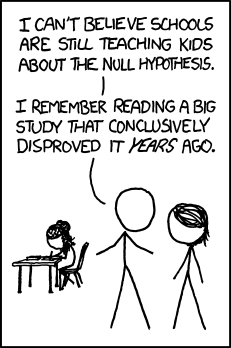
\includegraphics[width=\linewidth]{figures/xkcd-null_hypothesis}
  \caption{\url{http://xkcd.com/892/}: 
    Hell, my eighth grade science class managed to
    conclusively reject it just based on a classroom experiment.
    It's pretty sad to hear about million-dollar research teams
    who can't even manage that.
  }
\end{marginfigure}


\section*{Notes to self}

\begin{itemize}
  \item Read/cite \textcite{gigerenzer2007}
\end{itemize}

%\chapter{\label{ch:formal-languages}Formal languages and automata}

Natural languages can hardly be considered `formal' languages.%
\sidenote{?? Quote from Montague: ``no important theoretical difference between natural languages and the artificial languages of logicians.''}
From a practical engineering perspective,
our efforts to come up with (hand-crafted) formal specifications of
languages often often resulted in sub-optimal results.
However, we learned a lot about trying to do so,
and many of the concepts/methods developed are at the hart of computer science,
and many (practical) methods we use in computational linguistics.

In this lecture,
we will go through a gentle introduction to the theory of computation.
Our focus will be on \emph{automata} and corresponding formal languages.
However, we will necessarily touch on the other two subfields of
theory of computation, \emph{computability} and \emph{complexity}.

\section{Some definitions: Languages, strings, grammars}

\newthought{An alphabet} is a set of symbols.
We often use letters for our examples,
so $\{a, b, c\}$ is an alphabet consisting of three letters.
For many problems we may be interested in a binary alphabet like $\{1, 0\}$.
And for some of natural language problems our alphabet may consist of words,
such as $\{\text{cat}, \text{dog}, \text{sat}, \text{on}, \text{mat}\}$.
By convention, the Greek capital letter sigma $\Sigma$ for representing 
an alphabet.

\newthought{A string} is a finite sequence of symbols from an alphabet.
$a$, $ac$ or $abcaab$
are example string over alphabet $\{a, b, c\}$.
A special string that does not contain any symbols,
the \emph{empty string} is denoted by Greek letter epsilon, $\epsilon$.
We denote the set of all string over $\Sigma$,
including the empty string, with $\Sigma^{*}$.
$\Sigma^{+}$ is often used for the set of non-empty string in $\Sigma^{*}$
(a shorthand for $\Sigma^{*} - {\epsilon}$).
Note that both $\Sigma^{*}$ and $\Sigma^{+}$ have infinite number of members.
We indicate the length of a string with vertical bars on both sides,
$\lvert{}ab\rvert = 2$, or if $u = 0100$, $\lvert{}u\rvert{} = 4$.
For two string $u$ and $v$, we indicate their concatenation with $uv$.
If $u = 0100$ and $v = 11$, $uv = 010011$.

\newthought{A language} is a set of strings over an alphabet.
Empty set, $\emptyset$, is a language,
as well as the set containing only the empty string $\{\epsilon\}$.
Similarly $\Sigma^{*}$ is another language over alphabet $\Sigma$.
We are generally interested in more interesting languages,
such as%
\sidenote{Although we define these languages informally here,
  all of them can be defined more formally.
  For example, the language by the first item
  can be defined as $\{u\mid \lvert{}u\rvert = 2\}$.}
\begin{itemize}
  \item The set of strings of length \num{2}
    over $\{0, 1\}$: $\{00, 01, 10, 11\}$
  \item The set of strings with even number of \num{1}'s over $\{0, 1\}$:
      $\{\epsilon, 101, 0, 11, 111110, \ldots\}$
  \item The set of string that retain alphabetical ordering
    over $\{a, b, c\}$: $\{a, ab, abc, ac, abcc, \ldots\}$
  \item The set of strings of words
    that form a grammatically correct English sentences
\end{itemize}
The strings that are in a language are called \emph{sentences} of the language.

\newthought{A grammar} is a finite description of a language.
Although the set-based definitions above is flexible,
it is more convenient to express a language with a finite set of rules.
The most common method for formalizing grammars is based on
a set of \emph{rewrite rules}.
A rewrite rule two sides delimited by an arrow ($\ra$).
The grammar generates strings in the language,
by rewriting sequence of symbols matching right-hand-side (RHS) of the rule 
as the left-hand-side (LHS) of the rule,
starting from a special `start' symbol denoted by `S'.
The sequences of symbols in a rewrite rule is may consist of
\emph{terminal} symbols that are member of the alphabet
and \emph{non-terminal} symbols.
The non-terminal symbols are denoted using capital letter by convention.
For example, the grammar in Figure~\ref{fig:exmpl-grammar}
produces a language over the alphabet $\{a, b, c\}$
whose last symbol (word) is always an $a$.
This is not the only way to express the same language.
There are multiple (better, more concise) ways of writing
the same grammar.
The rule number 2\ in the grammar shown in Figure~\ref{fig:exmpl-grammar}
is recursive, it allows infinite number applications of this rule,
and hence, the grammar defines an infinite language with a finite set of rules.

\begin{marginfigure}
  \begin{tcolorbox}
    \begin{enumerate}
      \item $ S \ra A a$
      \item $ A \ra B A$
      \item $ A \ra B$
      \item $ B \ra a$
      \item $ B \ra b$
      \item $ B \ra c$
    \end{enumerate}
  \end{tcolorbox}
  \caption{\label{fig:exmpl-grammar}%
    An example grammar producing string over $\{a, b, c\}$
    that end with symbol $a$.
    A common short-hand for writing last three rules is a single rule 
    of the form `$B \ra a | b | c$'.
  }
\end{marginfigure}

Formally,
a phrase structure grammar is a tuple
$G = (\Sigma, N, S, R)$, where
  \begin{itemize}
    \item[$\Sigma$] is an alphabet of terminal symbols
    \item[$N$] are a set of non-terminal symbols 
    \item[$S$] is a special `start' symbol $\in N$
    \item[$R$] is a set of rules of the form $\alpha \ra \beta$,
      where  $\alpha$ and $\beta$ are strings from $(\Sigma \cup N)^{*}$.
  \end{itemize}

For our example in Figure~\ref{fig:exmpl-grammar},
$\Sigma = \{a, b, c\}$, $N = \{S, A, B\}$, $S = S$,
and $R = \{ S \ra A a, A \ra B A, A \ra B,
      B \ra a, B \ra b, B \ra c\}$.


\begin{marginfigure}
  \begin{tcolorbox}[halign=center]
    \begin{tabular}{l@{\Ra}ll}
      $S      $ & $A a$     &(rule 1)\\
      $A a    $ & $B A a$   &(rule 2)\\
      $B A a  $ & $B B A a$ &(rule 3)\\
      $B B A a$ & $B B B a$ &(rule 3)\\
      $B B B a$ & $B B c a$ &(rule 6)\\
      $B B c a$ & $B b c a$ &(rule 5)\\
      $B b c a$ & $a b c a$ &(rule 4)\\
    \end{tabular}
  \end{tcolorbox}
  \caption{\label{fig:example-derivation}%
    A derivation of string $abca$ using the grammar
    in Figure~\ref{fig:exmpl-grammar}.
  }
\end{marginfigure}
Given the grammar in Figure~\ref{fig:exmpl-grammar},
the string \texttt{abca} can be derived with the derivation sequence
presented in Figure~\ref{fig:example-derivation}.
We could write the same derivation sequence as
'$S \Ra A a \Ra B A a \Ra B B A a \Ra B B B a \Ra B B c a \Ra B b c a \Ra a b c a$'.
In general, if a string can be derived from the start symbol S
using a sequence of rewrite rules as above
(sometimes notes as `S $\overset{*}{\Ra}$ a b c a',
we say that the grammar \emph{generates} the string,
or the string is \emph{recognized} by the grammar.
Hence, the string is a valid sentence in the language.

The above definitions are important for understanding formal languages,
and also used in study of natural languages in formal linguistics.

\section{Chomsky hierarchy of languages}

\begin{marginfigure}
  \begin{center}
    \tikzset{external/export next=false}%
    \begin{tikzpicture}[x=4mm,y=8mm]
      \draw (0,0) ellipse (3.0 and 1.0);
      \node[font=\footnotesize] at (0,0) {Regular};
      \draw (0,0.5) ellipse (4.0 and 1.5);
      \node[font=\footnotesize] at (0,1.3) {Context Free};
      \draw (0,1.0) ellipse (5.0 and 2.0);
      \node[font=\footnotesize] at (0,2.3) {Context Sensitive};
      \draw (0,1.5) ellipse (6.0 and 2.5);
      \node[font=\footnotesize] at (0,3.2) {Recursively Enumerable};
      \draw (-6.1,-1.1) rectangle (6.1,4.1);
      %\draw (4,3.8) node {All};
    \end{tikzpicture}
  \end{center}
  \caption{\label{fig:chomsky-h}%
    Chomsky hierarchy of language classes. 
    The classes are also known as \emph{type-0}
    (recursively enumerable) to \emph{type-3} (regular).
  }
\end{marginfigure}

The Chomsky hierarchy of languages
is one of Chomsky's most important contributions
to both linguistics and computer science \parencite{chomsky1959b}.
For his theory of natural language syntax,
Chomsky defined a set of formal language classes
(depicted in Figure~\ref{fig:chomsky-h}).
Each class in this hierarchy is the proper subset of the larger class.
The larger classes are more descriptive,
but their computational processing is more demanding.
This particular classification of the language classes
has some attractive formal properties,
and each class corresponds to
a certain type of abstract computational device
that is capable of recognizing
and generating the languages in the corresponding class.
As a result, as well as its importance for (computational) linguistics,
this hierarchy is also an important part theory of computation.
We will define the individual language classes and the
properties of the rewrite grammars that expresses them.
In general, we will describe each language class
based on the restriction they put in the rewrite grammars that describe them.

We will next discuss at these language classes with in detail.
However, we note that these language classes are not 
the only formally defined language classes.
There are other well-studied language classes
some of which can be placed
in the set-inclusion hierarchy in Figure~\ref{fig:chomsky-h},
while other may cross-cut parts of this hierarchy.

\subsection{A brief divergence: complexity theory}

As noted earlier,
study of formal languages strongly linked to theory of computation,
particularly complexity theory.
Here, we will briefly review a part of the complexity theory briefly,
since some of the concepts will be instrumental in our discussion
of the language classes and the computational problems
related to these language classes.

In analysis of algorithms,
and algorithms worst time order of complexity 
is indicated a notation called \emph{big-O notation}.
Big-O notation aims to measure an algorithms complexity
as its input grows in size.
Since the aim of the big-O notation is indicating
the worst case with large number of input,
we discard all constant and lower order complexities from
the analysis of our algorithm.
For example, if our analysis indicate an algorithm to require
$T(n) = 100\times{}2^{n} + n^{10} + \log{n} + 10^{100}$ steps
(e.g., a simple operation on a CPU) to complete,
the complexity we are interested in is indicated by $O(2^{n})$.
In general, we drop all terms except $2^{n}$ above,
since all other figure will dwarfed by this term
as the size of the input ($n$) is increased.
Although even a constant factor is often important in practice,
we may be able get reasonable running times by parallelization,
or hope that increase in computing power will allow us
to use these algorithms.
The order of complexity measured with big-O notation has
more important theoretical consequences.
A few common examples of complexities measured using big-O notation
are given below.

\begin{itemize}[nosep,labelindent=1em,labelwidth=1.3cm,labelsep*=1em,leftmargin =!]
  \item[\textcolor{blue!50!green}{$O(1)$}] constant,
    an algorithm that does not depend on the size of its input,
    e.g., accessing a single element of an array
  \item[\textcolor{blue!50!green}{$O(\log n)$}] logarithmic,
    e.g., binary search
  \item[\textcolor{blue!50!green}{$O(n)$}] linear,
    e.g., finding minimum or maximum value of an array
  \item[\textcolor{blue}{$O(n \log n)$}] log linear,
    e.g., some sorting algorithms 
  \item[\textcolor{blue}{$O(n^{2})$}] quadratic,
    e.g., selection sort (and most arithmetic operations)
  \item[\textcolor{blue}{$O(n^{3})$}] cubic
  \item[\textcolor{red}{$O(2^{n})$}] exponential,
    e.g., graph search algorithms involving backtracking
    (note that the base is not important)
  \item[\textcolor{red}{$O(n!)$}] factorial,
    e.g., enumerating all binary trees spanning $n$ items (words)
\end{itemize}

\begin{marginfigure}
  \begin{tikzpicture}
    \begin{axis}[
        ymax=2000,
        axis x line=bottom,
        axis y line=left,
        xlabel=$n$,
        xlabel style={font=\tiny},
        ylabel style={font=\tiny},
        title style={font=\tiny},
        ticklabel style={font=\tiny},
        x=0.4mm,
        y=0.025mm,
%        cycle list={colormap/Spectral-7},
        thick,
        grid,
        legend style={font=\tiny,fill=none,draw=none},
        legend cell align=left,
      ]
      \addplot[blue,dashed, domain=1:100, samples=100] {ln(x)};
      \addplot[green,domain=1:100, samples=100] {x};
      \addplot[black,dashed, domain=1:100, samples=100] {x*ln(x)};
      \addplot[orange,domain=1:100, samples=100] {x^2};
      \addplot[brown,dashed,domain=1:15, samples=100, smooth,unbounded coords=jump] {x^3};
      \addplot[purple,domain=1:12, samples=100, smooth,unbounded coords=jump] {2^x};
      \addplot[red,dashed,domain=1:8, samples=7, unbounded coords=jump] {x!};
      \legend{
          $O(\log n)$,
          $O(n)$,
          $O(n \log n)$,
          $O(n^{2})$,
          $O(n^{3})$,
          $O(2^{n})$,
          $O(n!)$,
      };
    \end{axis}
  \end{tikzpicture}
  \begin{tikzpicture}
    \begin{semilogyaxis}[
        ymax=1000000000000000000000000000,
        ytickten={0,5,...,25},
        axis x line=bottom,
        axis y line=left,
        xlabel=$n$,
        xlabel style={font=\tiny},
        ylabel style={font=\tiny},
        title style={font=\tiny},
        ticklabel style={font=\tiny},
        x=0.4mm,
        y=0.75mm,
%        cycle list={colormap/Spectral-7},
        thick,
        grid,
        legend style={font=\tiny,fill=none,draw=none, yshift=-1cm},
        legend cell align=left,
      ]
      \addplot[blue,dashed, domain=1:100, samples=100] {ln(x)};
      \addplot[green,domain=1:100, samples=100] {x};
      \addplot[black,dashed, domain=1:100, samples=100] {x*ln(x)};
      \addplot[orange,domain=1:100, samples=100] {x^2};
      \addplot[brown,dashed,domain=1:100, samples=100, smooth,unbounded coords=jump] {x^3};
      \addplot[purple,domain=1:100, samples=100, smooth,unbounded coords=jump] {2^x};
      \addplot[red,dashed,domain=1:30, samples=30, unbounded coords=jump] {x!};
      \legend{
          $O(\log n)$,
          $O(n)$,
          $O(n \log n)$,
          $O(n^{2})$,
          $O(n^{3})$,
          $O(2^{n})$,
          $O(n!)$,
      };
    \end{semilogyaxis}
  \end{tikzpicture}
  %TODO: more print-friendly graphs
  \caption{\label{fig:computational-complexity}%
    Order of operations required by different algorithmic complexity
    measured by big-O notation.
    Top graph represents this linearly,
    while the y-axis of bottom graph is logarithmic
    (changes in the graph indicate an exponential changes
    in the number of operations),
    allowing us to visualize later compare complexity over
    a larger interval of input size $n$.
  }
\end{marginfigure}
Naturally, we prefer the lower-complexity algorithms
(earlier items in the above list).
However, the behavior of the last two items in the list
and the earlier ones are drastically different when the input size is increased.
The ones up to $O(n^{3})$ above,
in general any algorithm whose complexity can be explained
a polynomial of any degree,
are called \emph{polynomial} time algorithms.
In general, polynomial time algorithms are said to be \emph{tractable}.
And algorithms with worse complexity than polynomial time
are called \emph{intractable}.
Intractable algorithms scale badly with increased input size,
Even with reasonable increase in computing power,
we do not have any hopes of solving intractable algorithms
for larger input sizes.
Figure~\ref{fig:computational-complexity}
presents order of operations needed for algorithms
with different complexities.
The top graph in Figure~\ref{fig:computational-complexity},
showing how drastic the complexity may change.
Note that an algorithm with $O(n^{3})$ requires more operations
for small input sizes,
but in time non-polynomial algorithms more costly for larger input sizes.
The bottom graph shows this more drastically,
as the input size increased,
the polynomial and non-polynomial algorithms becomes much clear.

A fundamental activity in computer science is to find
algorithms with lower big-O complexity.
For example,
a brute-force approach to recognizing context-free languages 
is exponential in the length of the sentence (or computer program).
However, we have clever solutions that work in polynomial time
using a modest amount of additional storage.
The class of problems that has a known polynomial-time algorithm is
indicated by P.
For some problems we do not know a tractable algorithm.
However, they are not provably intractable,
we may hope to find some polynomial time algorithm for solving
these problems and they may become a member of P.
An interesting subclass of these problems
for which we do not have a polynomial-time algorithm to solve it,
we can identify the solution (in polynomial time) when we see the solution.
This class of problems are called
\emph{non-deterministic polynomial time} (NP).
P is a subset of NP.
However, one of the big questions in theory of computation is
whether P is equal to NP or not.
If it is,
then there are tractable algorithms waiting to be discovered
for many of the problems in NP.

An interesting sub-class of NP is called NP-complete.
If we find a polynomial time solution to any of the NP-complete problems,
we can solve all NP problems in polynomial time,
since solution of any NP problem can be `converted' obtained using
the solution of an NP-complete problem
with a polynomial overhead for the conversion.
Finding a polynomial algorithm for an NP-complete problem
would prove P = NP,
as well as solving many difficult problems in a wide range of fields.
However, 
the fact we do not know tractable algorithms for NP-complete problems
despite decades of efforts by many clever people
suggests that P is probably not equal to NP.
Hence, when we face a problem that is NP-complete,
or in a more difficult complexity class,
chances of finding a scalable solution is rather unlikely.

The concepts introduced above should be sufficient to understand
some of the complexity issues we will discuss below.
However, there are many other complexity classes,
and many unknowns, interesting problems,
about the relation between these classes.
A reasonable overview of computational complexity is
out of the scope of this lecture.
The additional resources at end of the chapter points to
a few textbooks covering the complexity theory is covered.

\subsection{Regular languages}

Regular languages is the simplest
(least expressive, easy to process computationally)
class in Chomsky hierarchy.
The regular languages are defined by \emph{regular grammars}
which are (mostly) equivalent to \emph{regular expressions}
that are used in many programming environments
for searching patterns in text.
We will study regular languages in detail in Chapter~\ref{ch:fst}.

\begin{marginfigure}
  \begin{tcolorbox}[rounded corners]
    \begin{multicols}{2}
      \begin{enumerate}
        \item $A \ra a$
        \item $A \ra Ba$
        \item $A \ra \epsilon$
      \end{enumerate}
      \begin{enumerate}
        \item $A \ra a$
        \item $A \ra aB$
        \item $A \ra \epsilon$
      \end{enumerate}
    \end{multicols}
  \end{tcolorbox}
  \caption{\label{fig:regular-grammars}%
    The possible rules for left-regular (left)
    and right-regular (right) grammars.
    For both, $A$ and $B$ are non-terminal,
    $a$ is a terminal sybol ($a \in \Sigma$),
    and $\epsilon$ is the empty string.
  }
\end{marginfigure}
A \emph{regular grammar} is a grammar that generates a regular language.
There are two flavors of regular grammars.
The \emph{left-regular grammars} can have only the rules listed in left side
of Figure~\ref{fig:regular-grammars}.
The rules allowed in a \emph{right-regular grammar} is listed
in the right side of Figure~\ref{fig:regular-grammars}.
In simple words, regular grammar can have three types of rules
\begin{itemize}
  \item A single non-terminal symbol rewritten as a single terminal symbol
  \item A single non-terminal symbol as one terminal
    and one non-terminal symbol
    (the order determines whether the grammar left or right regular)
  \item A single non-terminal symbol as empty string ($\epsilon$)
\end{itemize}
Note that both definitions allow defining all (and only) regular languages.
Some definitions do not allow transition to empty string
(3rd rule in both definitions).

A regular grammar only defines regular languages.
However, note that regular languages can also be defined
with non-regular grammars (e.g., context free grammars we will define next).

%TODO: examples, exercises

\subsection{Context-free languages}

Context-free languages are the next (more expressive) language
after regular languages in the Chomsky hierarchy.
They are used in describing (and parsing) programming languages.
The syntax of all programming languages are based on context-free grammars.%
\sidenote{They are generally defined by a restricted
  (deterministic, non-ambiguous) subset of context-free grammars
  for efficiency of parsing,
  and in a limited/restrict set of non-context freeness may be used. 
}
Similarly,
many syntactic theories of natural languages are based on
a context-free backbone
(we will discuss this further in Section~\ref{sec:nl-and-fl}).

The restrictions on the rewrite rules
for context-free grammars are simple:
left-hand-side (LHS) of the rule has to contain a single non-terminal.
Unlike regular grammars,
we do not have any restrictions on right-hand-side (RHS)
of the rewrite rules.
They can contain any combination of non-terminal and terminal symbols
(or $\epsilon$).
The context-free languages are called so,
since the rewrite rules express
expanding a non-terminal anywhere independent of their context.

%TODO: examples, exercises

\subsection{Context sensitive languages}

Context sensitive languages are a superset of context-free languages.
The rules of context sensitive language are required to be in the following form.
\[
  \alpha A \beta \ra \alpha \gamma \beta
\]
where $A$ is a single non-terminal symbol,
$\alpha$ and $\beta$ are
possibly empty strings of terminals and non-terminals,
and $\gamma$ is a non-empty string of terminal and non-terminal symbols.
Note that the above definition does not allow
a LHS non-terminal to be deleted (rewritten as $\epsilon$).
However, a rule of the form $S \ra \epsilon$ is allowed
to ensure that the context-sensitive languages are
a superset of context-free languages.
Another way to define a context sensitive grammars is 
requiring the RHS of all rules to be longer than or equal to the LHS.%
\sidenote{The grammars defined this way is known as
  \emph{non-contracting grammars} and are
  known to be \emph{weakly equivalent} to context-sensitive grammars.
  That is, we can convert any non-contracting grammar to 
  a context-sensitive grammar.
}

Many problems with context-sensitive grammars do not have
efficient solutions (see Section~\ref{sec:formallang-automata}).

\subsection{Recursively enumerable languages}

The recursively enumerable languages are the most expressive language
in the Chomsky hierarchy.
Recursively enumerable languages are languages over an alphabet that are,
well, recursively enumerable.
That is, there exist an algorithm that can enumerate (list)
all strings in the language.

The grammars that define recursively enumerable languages
do not pose any restrictions on their rewrite rules,
except that their LHS being non-empty.
The class of grammars that generate recursively enumerable languages
are called \emph{unrestricted grammars}.

\section{\label{sec:formallang-automata}Formal languages and automata}

The simplest question we ask about a grammar,
or the corresponding language,
is recognizing strings that belong to the language.
That is, given a string,
can we determine whether it belongs to the language or not?

This question links the language classes described above to
abstract computation devices, \emph{automata}.
In other words,
for each language class discussed above,
there is an type of automaton that recognizes the strings of
a language in the class.
We will briefly discuss these correspondences,
starting from the most-expressive language class.

Strings in a recursively enumerable language,
the most expressive class in the Chomsky hierarchy,
can be recognized by a \emph{Turing machine}.
The Turing machine is a simple abstract computing device
that can compute any computable function.
In other words, any algorithm can be simulated by a Turing machine.
The relationship between recursively enumerable languages
and Turing machines mean
that a Turing machine can generate all (and only) string
in the corresponding recursively enumerable language.
However, the question is whether a string is in
a recursively enumerable language or not is undecidable,
since it is equal to a \emph{halting problem},
a well known undecidable problem.

The machines that recognize the context-sensitive languages
are a restricted version of Turing machines
called \emph{linear-bounded automata}.
Although whether a string is generated by a context-sensitive grammar
or not is decidable,
it is known to be computationally complex.%
\footnote{More formally,
  it is PSPACE-complete, and PSPACE is a superset of NP.
}

Context-free grammars can be recognized by \emph{push-down automata}.
A push-down automaton has a finite number of sates that controls
the computation
(similar to the finite-state machines we will summarize next),
and a stack (with access to only the top element) as memory.
Although the complexity of first two
the grammars and machines discussed above are computationally intractable,
there are many practical algorithms for solving problems
involving context-free grammars.
We will revisit the context-free grammars
when we discuss parsing algorithms later.

\begin{marginfigure}
  \begin{center}
    \begin{tikzpicture}[
      ]
      \node[draw,thick,state,initial,initial text={}] (s0) {0};
      \node[draw,thick,right=of s0,state] (s1) {1};
      \node[draw,thick,right=of s1,state,accepting] (s2) {2};
      \draw[->] (s0) edge[above] node{a} (s1)
                (s1) edge[loop above] node{b} (q1)
                (s1) edge[above] node{c} (s2);
    \end{tikzpicture}
  \end{center}
  \caption{\label{fig:fsa-example}%
    An example automata recognizing the strings over alphabet
    $\{a, b, c\}$ which begins with $a$, followed by zero or more
    $b$s, and ends with $c$.
  }
\end{marginfigure}
Finally, the regular languages are recognized by finite-state automata.
Finite state automata (FSA) can be described by a directed graph
with a finite nodes (states) and edges are
labeled with symbols of the alphabet.
A finite-state automaton
can accept (or rejects) its input in time complexity
linear in the length of input.
Furthermore, the FSA are `memoryless',
except the automaton itself, they do not need any additional memory.
Figure~\ref{fig:fsa-example} shows an example finite state automata.
We will discuss finite-state automata in Chapter~\ref{ch:fsa}.

\section{Where do natural languages fit}

One of the motivations behind building the classes of languages
in the Chomsky hierarchy was to characterize
the type of formal grammars that are adequate for natural languages,
primarily natural language syntax.
By `adequate', we mean classes of grammars that can represent
the phenomena we observe in natural languages,
yet computationally not so demanding.
The latter condition, computational efficiency,
is not only desirable
from the perspective of computational processing of natural languages.
It is also important for cognitive science
where one of the main tenets is that cognition is a form of computation.
Since human cognitive system is a computing device
with limited/finite resources,
there are bounds on its computational capabilities.
As a result, the computational efficiency of language processing is
also important for study of human languages from a cognitive perspective.


Initially,
context-free languages were considered to be adequate
for representing natural languages.
However,
a small number of linguistic constructions cannot be represented
using context-free languages.
A typical example is the cross-serial dependencies found
in Dutch and Swiss German.
Figure~\ref{fig:cross-serial} presents
an example cross-serial dependency from Swiss German.
The dependencies with the verbs and their arguments cross.
As a result, context free grammars cannot represent this structure.
The problem is clearer if you consider
the operations of a push down automaton.
If we push the case marking on each noun on the stack,
by the time we process the verb \xmpl{hälfed},
we do not have access to case marking of its argument
as it is not on the top of the stack anymore.

\begin{figure*}
  \tikzset{external/export next=false}
  \begin{center}
    \begin{tikzpicture}
      \matrix[matrix of nodes] (m) {
        Jan & säit  & das & mer &\color{blue} em Hans & \color{red}es huss & \color{blue} hälfed & \color{red}aastriiche \\
        Jan & said & that & we & Hans (\textsc{dat}) & the house (\textsc{acc}) & helped & paint \\
      };
      \draw[blue] (m-1-5) to[in=north, out=north, looseness=0.5] (m-1-7);
      \draw[red] (m-1-6) to[in=north, out=north, looseness=0.5] (m-1-8);
    \end{tikzpicture}
  \end{center}
  \caption{
    An example cross-serial dependency from Swiss German
    \parencite{shieber1985}.
    The case marking of \xmplt{em Hans}{Hans} agrees with the verb
    \xmplt{hälfed}{helped},
    while the case marking of \xmplt{es huss}{house} agrees with the verb
    \xmplt{aastriiche}{paint}.
    Note that this resembles 
    $a^{\color{blue}n}b^{\color{red}m}c^{\color{blue}n}d^{\color{red}m}$.
  }\label{fig:cross-serial}%
\end{figure*}

Although the syntactic phenomena such as the one presented
in Figure~\ref{fig:cross-serial} are clearly non-context free,
their existence do not require the full representation power
(and computational complexity) of context-sensitive grammars.
A common theoretical consensus seems that
a grammar class, called \emph{mildly context sensitive} grammars
are adequate for representing natural languages
(see Figure~\ref{fig:chomsky-h-mcs}).
In practice,
many computationally oriented theories of grammars use
a context-free backbone with some extensions that increase their
expressive power.
This extension may range from mildly context-sensitive grammars%
\sidenote{E.g., Combinatory categorial grammar (CCG)
and tree adjoining grammar (TAG).}
to Turing machine equivalence.%
\sidenote{E.g., Head-driven phrase structure grammars (HPSG),
  and (according to some analyses lexical-functional grammar (LFG).
}
Although these extensions increase
their worst-case computational complexity drastically,
these formalisms often work acceptably in practice due to their
reasonable expected/average time complexity.


Before closing this brief discussion of natural languages
and formal languages,
their representational power and computational complexity,
we should note that the non-context-free extensions
to the theories of natural language grammars are not
motivated only by the representation power.
Besides being able to represent the constructions
like the cross-serial dependencies,
extensions requiring higher
than context-free power are often proposed
when they match better with linguistic intuitions.
In other words, even if a context-free grammar may be adequate
to represent a language,
an extended version may match the linguists' intuition
of how the linguistic structures are derived better.

\begin{marginfigure}
  \begin{center}
    \tikzset{external/export next=false}%
    \begin{tikzpicture}[x=4mm,y=8mm]
      \draw[dashed] (0,.6) ellipse (4.2 and 1.6);
      \draw (0,0) ellipse (3.0 and 1.0);
      \node[font=\footnotesize] at (0,0) {Regular};
      \draw (0,0.5) ellipse (4.0 and 1.5);
      \node[font=\footnotesize] at (0,1.3) {Context Free};
      \draw (0,1.0) ellipse (5.0 and 2.0);
      \node[font=\footnotesize] at (0,2.4) {Context Sensitive};
      \draw (0,1.5) ellipse (6.0 and 2.5);
      \node[font=\footnotesize] at (0,3.2) {Recursively Enumerable};
      \draw (-6.1,-1.1) rectangle (6.1,4.1);
      %\draw (4,3.8) node {All};
    \end{tikzpicture}
  \end{center}
  \caption{\label{fig:chomsky-h-mcs}%
    A depiction of Chomsky hierarchy of language classes
    (Figure~\ref{fig:chomsky-h},
    with the addition of \emph{mildly context-sensitive languages}
    represented with the dashed ellipse.
  }
\end{marginfigure}

\section{\label{sec:formal-lang-learnability}%
        Formal languages and learnability}

A central question in modern linguistics, surrounded with a big debate,
has been learnability of natural languages.
Some researchers, primarily based on Noam Chomsky's ideas,
championed the idea that the natural languages are not learnable.
Hence, only way for a human child to learn the languages they are exposed to
is to have an innate linguistic component.
The debate is linked to an even bigger, and much older one:
nature vs.\ nurture debate. 
The debate at large  has little practical use in a course
on natural language processing.
It also seems the heated discussion on the topic has slowed down after 2000s.
However, part of the debate is linked with some of the results regarding
learnability of classes of formal languages,
and together with the fact that this discussion has
a historical significance in the field,
it deserves a brief mention here.

There has been a number of formal proofs
indicating that none of the languages in the Chomsky hierarchy is
learnable only from positive examples.%
\footnote{Mainly due to \textcite{gold1967}.}
These results frequently used as an argument for the innateness hypothesis.
However, the formal arguments are often too general,
and do not necessarily match the settings in which children learn languages.
For example, the results cited above are obtained for the language classes
in the Chomsky hierarchy,
while the human languages do not necessarily match with
one of these language classes.
It is more likely that the class of natural languages,
if such a class exists,
cross cut the hierarchy (as in Figure~\ref{fig:chomsky-h-cross}).
In other words,
even regular languages allow some constructions
that are not useful for representing structures in human languages.
%TODO: example
Furthermore,
the condition that the languages should be learned from
the positive examples alone is likely to be too strict
for a realistic setting for child language acquisition.

\begin{marginfigure}
  \begin{center}
    \tikzset{external/export next=false}%
    \begin{tikzpicture}[x=4mm,y=8mm]
      \definecolor{vlgray}{rgb}{0.9,0.9,0.9}
      \filldraw[vlgray,draw opacity=0.1] (0,.6) ellipse (1.5 and 1.6);
      \draw[dashed] (0,.6) ellipse (4.2 and 1.6);
      \draw (0,0) ellipse (3.0 and 1.0);
      \node[font=\footnotesize] at (0,0) {Regular};
      \draw (0,0.5) ellipse (4.0 and 1.5);
      \node[font=\footnotesize] at (0,1.3) {Context Free};
      \draw (0,1.0) ellipse (5.0 and 2.0);
      \node[font=\footnotesize] at (0,2.4) {Context Sensitive};
      \draw (0,1.5) ellipse (6.0 and 2.5);
      \node[font=\footnotesize] at (0,3.2) {Recursively Enumerable};
      \draw (-6.1,-1.1) rectangle (6.1,4.1);
      %\draw (4,3.8) node {All};
    \end{tikzpicture}
  \end{center}
  \caption{\label{fig:chomsky-h-cross}%
    A possible set (indicated by the shaded region in the figure)
    for class of natural languages in the Chomsky hierarchy,
    to demonstrate that learnability results on a particular language
    class in the hierarchy is not necessarily
    a positive or negative indication for learnability of natural languages. 
    As in Figure~\ref{fig:chomsky-h-mcs},
    the dashed ellipse represents
    the class of mildly context-sensitive languages.
  }
\end{marginfigure}

Perhaps more interesting for computational linguistics is
the question of learnability of languages is an empirical question
that can be answered by a computational model.
Theoretical claims aside,
if we can build models that can learn natural languages
from the input available to children,
that is a good indication that they are learnable.
Even if the computational model may not mimic
the way children learn languages,
they can be used to show that learning is in principle possible.
Furthermore,
if we constrain such models the way human learners are constrained,
we may be able to answer even more interesting questions.

In summary,
although it is not part of the mainstream
computational linguistics or natural language processing fields,
the methods used typically in these fields can also be instrumental
in study of languages from cognitive science perspective.

\section{Where to go from here}

This lecture is a brief overview of formal languages
and automata theory.
We also noted some topics in theory of computation
(e.g., computational complexity and complexity classes),
and even some related issues in theoretical linguistics
and cognitive science.
All of these topics are, necessarily, covered briefly, on the surface.
Some of these topics will be revisited in later lectures.
Here, we point to some of the relevant literature.

\textcite{hopcroft1979} (and its successive editions) has been
the most influential textbook on formal languages and automata theory.
\textcite{sipser2006} is another good textbook
on the topic
covering formal languages and automata as well as 
complexity theory and other interesting issues in the theory of computation.

The discussion of learnability
briefly touched in Section~\ref{sec:formal-lang-learnability}
started in 1950s and 1960s based on Chomsky's work.
The literature in the field is vast,
ranges from psycholinguistics to computational linguistics.
Probably most popular work
on the innateness side of the debate is \textcite{pinker1994},
focusing mainly claims based on theoretical and experimental work.
\textcite{a.clark2011book} provides a more recent review of the field
from the opposite side of the debate.
This book also is more closely related
to the formal languages discussed in this chapter.

\section{What to add}

\begin{itemize}
  \item About complexity: infinity is overrated
  \item A bit of clarification/emphasis on `generative' side of grammars
\end{itemize}

%%\chapter{\label{ch:fsa}Finite state automata and regular languages}

The regular languages, the simplest class of languages
we defined in Chapter~\ref{ch:formal-languages},
and the corresponding abstract machines, finite state automata (FSA), 
have many practical uses ranging from circuit design to string search.
They are also an important tool for computational linguistics.
In this chapter we will study FSA and regular languages.

%TODO: applications - dictionaries, shallow parsing ...

%TODO: link to regular expressions

\section{Finite state automata}

A finite state automaton is an abstract machine with a finite number of states.
The machine can be in one of the states in a given time,
and it changes its sates as it processes an input string
from a finite alphabet.
If the machine is in one of final or accepting states at the end of the input,
it accepts the string.
As noted earlier, finite state automaton
recognize and generate regular languages.
A finite state automaton accepts all and the only strings
that are in the corresponding regular language.

\begin{marginfigure}
  \begin{center}
    \tikzset{external/export next=false}
    \begin{tikzpicture}[every initial by arrow/.style={thick},
      ]
      \node[draw,state,initial,initial text={}] at (0,0) (s0) {0};
      \node[draw,above right=of s0,state] (s1) {1};
      \node[draw,below right=of s0,state,accepting] (s2) {2};
      \draw[->,thick,>=stealth]
                (s0) edge[above,bend left] node (nl) {b} (s1)
                (s0) edge[below,bend right] node{a} (s2)
                (s1) edge[loop above] node{b} (q1);
      \draw[->,thick,>=stealth]
                (s1) edge[right,bend left=90] node{c} (s2);
      \node[blue] at (-1, -1) (ilab) {initial state};
      \draw[blue,->,shorten >=1pt]  (ilab) to[bend right] (s0);
      \node[blue] at (-1, 1) (tlab) {transition};
      \draw[blue,->,shorten >=1pt]  (tlab) to[bend left] (nl.south);
%      \draw[blue,->,shorten >=1pt]  (tlab) to[bend left] ($(s0)!0.5!(s1)$);
      \node[blue] at (0, 2) (slab) {state};
      \draw[blue,->,shorten >=1pt]  (slab.east) to[bend left] (s1.north west);
      \node[blue] at (0, -2) (flab) {accepting state};
      \draw[blue,->,shorten >=1pt]  (flab) to[bend right] (s2);
    \end{tikzpicture}
  \end{center}
    \caption{\label{fig:example-fsa}%
      An example finite-state machine.
    }
\end{marginfigure}
A common way to think about (and represent) an FSA is a directed graph,
where the nodes correspond to the states,
and edges are labeled with the symbols from the alphabet.
Figure~\ref{fig:example-fsa} presents an FSA represented as
a directed graph.
The machine starts at the start state (marked with an incoming arrow)
and moves between the states based on the given input.
If the machine is in a final state
(represented as a double circle)at the end of the input,
the input string is accepted.

\subsection{Deterministic finite automata}
Formally, a finite state automaton, $M$,
is a tuple $(\Sigma,Q, q_{0}, F, \Delta)$ with

\begin{itemize}[nosep]
  \item[$\Sigma$] is the alphabet, a finite set of symbols
  \item[$Q$] a finite set of states
  \item[$q_{0}$] is the start state, $q_{0} \in Q$
  \item[$F$] is the set of final states, $F \subseteq Q$
  \item[$\Delta$] is a function that takes a state and a symbol in the alphabet,
    and returns another state ($\Delta: Q\times\Sigma \ra Q$)
\end{itemize}

The important part of the this definition is the last item,
translates to the requirement that given a state and a symbol,
there is only one possible state to go.
As a result,
a deterministic automata requires
exactly one edge labeled by each symbol in the alphabet leaving every state.


%\part{Basic NLP methods}
%\chapter{Tokenization, Segmentation, Normalization}

Almost any natural language processing application,
we use processing units such as sentences, words, morphemes.
These units, or linguistics objects,
are rarely available in clearly distinguishable form
even in well edited, high-quality text.
Identifying these units in the language data to be processed becomes
more difficult if one needs to process non-standard text or spoken language.
Furthermore,
different languages present different challenges.
For example,
some languages, such as Chinese and Japanese,
do not mark word boundaries in the written text,
which makes identifying words difficult.

These \emph{text processing} steps are essential for NLP systems.
Since the units identified in these stages are
input to the later stages of processing,
and any error at this stage will affect the usefulness of the NLP system.

\section{Document preprocessing}

\section{Tokenization}

\section{Segmentation}

\section{Normalization}


%\chapter{\label{chap:alignment}Sequence alignment}

\section*{Where to go from here}

%\chapter{\label{chap:ngram}N-grams}
%TODO: better chapter title

In this chapter we will study \emph{n-gram language models},
which we will call simply \emph{language models},
and sometimes we will even disregard
the distinction between the model and the sequence,
and call them \emph{n-grams}, following the common practice in the field.
The models we will discuss here are very simple,
yet very effective in many practical natural language applications.
The main idea is given a sequence of words,
we want to assign a probability to the sequence,
based on a short context of each word in the sequence.
These probabilities allow us to select the more likely sequence,
e.g., sentence or utterance, among other alternatives.
Before going into details,
we will motivate their use with a few examples.

\section{Example applications of n-gram language models}
Assume that you are developing a spell checker.
With a good enough lexicon,
it is not difficult to catch the spellling error in this sentence.
For morphologically complex languages,
you may need help from some morphological rules
to define the valid words in the language rather than listing them,
but once you have such a system that defines the valid words,
it is easy to spot spelling errors within words.
But, how about the spelling error in (\getref{spell-wit}) below?

\ex<spell-wit>
  I don't like pizza \emph{wit} spinach.
\xe

If we have a lexicon with word frequencies,
one way to to solve this problem would
be pay attention to \emph{confusables} of high-frequency words like \emph{with}.
Here, we may be able to rely on the fact that $P(\text{with}) > P(\text{wit})$.
This still does not solve the problem if the spelling correction is to be made non-interactively.
Choosing the high-frequency confusable does not guarantee correctness:
in another spelling error we may have \emph{with} instead of \emph{wit}.
Furthermore,
consider the news headline in (\getref{spell-lose}).

\ex<spell-lose>
  Zoo animals on the \emph{lose}
\xe

The word frequency (or probability) does not help here,
if you compare the frequencies of the words in Google Books Ngram Viewer,%
\footnote{\url{https://books.google.com/ngrams/graph?content=lose\%2C+loose}}
you will see that \emph{lose} has been more common
than the correct form in this example, \emph{loose},
in the most part of the history of written English.
Even though $P(\text{loose}) < P(\text{lose})$,
any competent speaker would agree that the relations between
the probabilities of complete sequences should be 
$P(\text{Zoo animals on the \emph{loose}}) > P(\text{Zoo animals on the \emph{lose}})$.
As a result,
we want our language model to assign probabilities to these sequences accordingly.

Those who took a parsing course before may (rightfully)
suggests parsing as a solution.
Indeed,
a structure-sensitive language model (e.g., a parser) would be helpful.
However,
parsing is a rather complex task.%
\footnote{Parsing is the most popular sport in computational linguistics.
  Like many sports, it is fun, but challenging -
  it is computationally `heavy' and requires resources (treebanks)
  that are expensive to build.
  Although we (computational linguists) have been enthusiastic about our sport,
  in most practical applications,
  simpler solutions (like the ones we will discuss in this chapter)
  often work better -
  or well enough that complexity of parsing is not warranted.
}
The n-gram models that we will discuss in this chapter are much simpler,
yet effective enough that they are the dominant method for language modeling
in many of the practical applications.
The basic idea is to estimate the probability of a sequence,
such as a sentence,
from its parts (the words),
and to estimate the probabilities of the words,
pay attention to the context of the word.

The spelling correction example above is not the only application for n-grams.
There are many applications of the n-gram language models.
For example,
in automatic speech recognition (ASR),
the speech signal often gives rise to multiple possible word sequences.
A well-known example is presented in Figure~\ref{fig:wreck},
where all possible word sequences that are compatible
with the \emph{phone}s identified from the speech signal are represented in a lattice.
Each path that spans all the phones is a candidate utterance,
among which we can trace \emph{wreck a nice beach},
as well as the expected \emph{recognize speech}.
Even if the former may be more likely based on the analysis of the signal,
an n-gram model scoring the sequences is likely to select the latter,
at least if the n-gram model was trained on language samples of NLP domain.
\begin{marginfigure}
  \tikzsetnextfilename{wreck-a-nice-beach}
  \begin{tikzpicture}[every node/.style={anchor=south,inner ysep=0.1em,font=\tiny},
                      x=5mm
    ]
    \foreach \x/\l in {0/r,1/e,2/k,3/@,4/n,5/ai,6/s,7/b,8/ii,9/ch}{%
      \draw ($ (\x, 0) + (0.5, 0) $)  node[anchor=base,font=\scriptsize] {\l};
    }

    \pgfsetcornersarced{\pgfpoint{2mm}{2mm}}
    \def\height{0.3}

    \pgfmathsetmacro{\y}{1*\height}
    \draw (3,0) -- (3,\y) -- node {her} (4,\y) -- (4,0);
    \draw (4,0) -- (4,\y) -- node {and} (5,\y) -- (5,0);
    \draw (5,0) -- (5,\y) -- node {I} (6,\y) -- (6,0);
    \draw (6,0) -- (6,\y) -- node {s} (7,\y) -- (7,0);
    \draw (7,0) -- (7,\y) -- node {be} (9,\y) -- (9,0);

    \pgfmathsetmacro{\y}{2*\height}
    \draw (3,0) -- (3,\y) -- node {a} (4,\y) -- (4,0);
    \draw (4,0) -- (4,\y) -- node {aren't} (5,\y) -- (5,0);
    \draw (5,0) -- (5,\y) -- node {ice} (6,\y) -- (6,0);
    \draw (7,0) -- (7,\y) -- node {bee} (9,\y) -- (9,0);

    \pgfmathsetmacro{\y}{3*\height}
    \draw (4,0) -- (4,\y) -- node {an} (5,\y) -- (5,0);
    \draw (5,0) -- (5,\y) -- node {eye} (6,\y) -- (6,0);
    \draw (7,0) -- (7,\y) -- node {beach} (10,\y) -- (10,0);

    \pgfmathsetmacro{\y}{4*\height}
    \draw (4,0) -- (4,\y) -- node {not} (5,\y) -- (5,0);

    \pgfmathsetmacro{\y}{5*\height}
    \draw (4,0) -- (4,\y) -- node {nice} (7,\y) -- (7,0);

    \pgfmathsetmacro{\y}{6*\height}
    \draw (3,0) -- (3,\y) -- node {an} (5,\y) -- (5,0);

    \pgfmathsetmacro{\y}{7*\height}
    \draw (3,0) -- (3,\y) -- node {aren't} (5,\y) -- (5,0);
    \draw (6,0) -- (6,\y) -- node {speech} (10,\y) -- (10,0);

    \pgfmathsetmacro{\y}{8*\height}
    \draw (3,0) -- (3,\y) -- node {in} (5,\y) -- (5,0);
    \draw (5,0) -- (5,\y) -- node {ice} (7,\y) -- (7,0);
    \draw (7,0) -- (7,\y) -- node {speech} (10,\y) -- (10,0);

    \pgfmathsetmacro{\y}{9*\height}
    \draw (0,0) -- (0,\y) -- node {wreck} (3,\y) -- (3,0);
    \draw (3,0) -- (3,\y) -- node {on} (5,\y) -- (5,0);

    \pgfmathsetmacro{\y}{10*\height}
    \draw (0,0) -- (0,\y) -- node {reckon} (5,\y) -- (5,0);

    \pgfmathsetmacro{\y}{11*\height}
    \draw (0,0) -- (0,\y) -- node {recognize} (7,\y) -- (7,0);
  \end{tikzpicture}
  \caption{\label{fig:wreck}%
    An automatic speech recognizer's attempt to recognize
    the phrase \xmpl{recognize speech}.
    Example re-produced from \parencite{shillcock1995}.
  }
\end{marginfigure}

A very similar use case also arise in machine translation (MT).
The classical statistical MT systems produce
many alignments between the source and target languages,
and a language model of the target language is used
for picking the most fluent option.
For example the German phrase \xmpl{Er tanzt gerne} can be translated as
`He dances with-pleasure' or `He likes to dance'.
Although both are acceptable translations,
a language model of English is expected to pick the more fluent (second) option.

% TODO:
% All three examples above are typically modeled
% using the noisy channel model discussed in Chapter~\ref{chap:information-theory}
% 
% \begin{marginfigure}
%   \tikzsetnextfilename{noisy-channel}
%   \begin{tikzpicture}
%     \node (in) {a};
%     \node[draw,thick,right=3mm of in, minimum height=4ex] (enc) {encoder};
%     \node[draw,thick,right=15mm of enc, minimum height=4ex] (dec) {decoder};
%     \node[right=3mm of dec] (out) {a};
%     \draw[thick,->] (in) -- (enc);
%     \draw[thick,->] (dec) -- (out);
%     \draw[thick,decorate, decoration={snake,post length=1mm},->]
%       (enc) -- (dec)
%       node[midway, above,yshift=2mm,font=\small,text width=1cm,align=center]
%         {noisy\\channel};
%   \end{tikzpicture}
%   \caption{\label{fig:noisy-channel}%
%   }
% \end{marginfigure}
% 

In the examples above,
we were interested in assigning probabilities (or scores) to a sequence of words.
Another application of the language models is in predicting the next word.
This is commonly used in text boxes in web applications,
such as query input of a search engine.
Note that although most of our examples were about words,
we may need to score sequences of other linguistic units,
such as letters or phonemes.
An example of predictive text based on letters is found
in mobile phone virtual keyboards,
which helps phone users typing short messages quickly.
Figure~\ref{fig:google-predictive-text} shows screenshots
from a web application with predictive text
using both word- and character-level models.
\begin{marginfigure}
  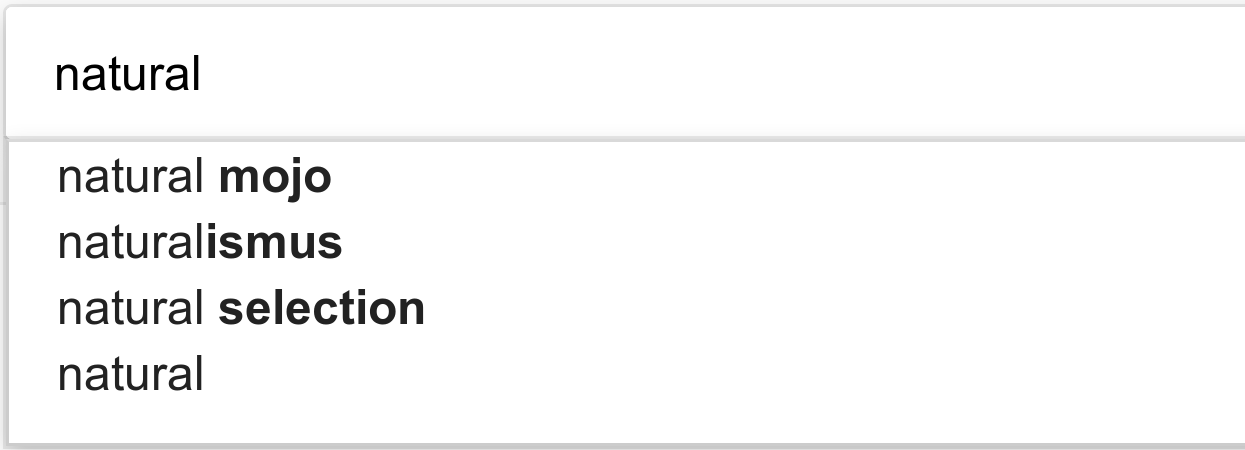
\includegraphics[width=\textwidth]{figures/google-predictive-text-1.png}\\
  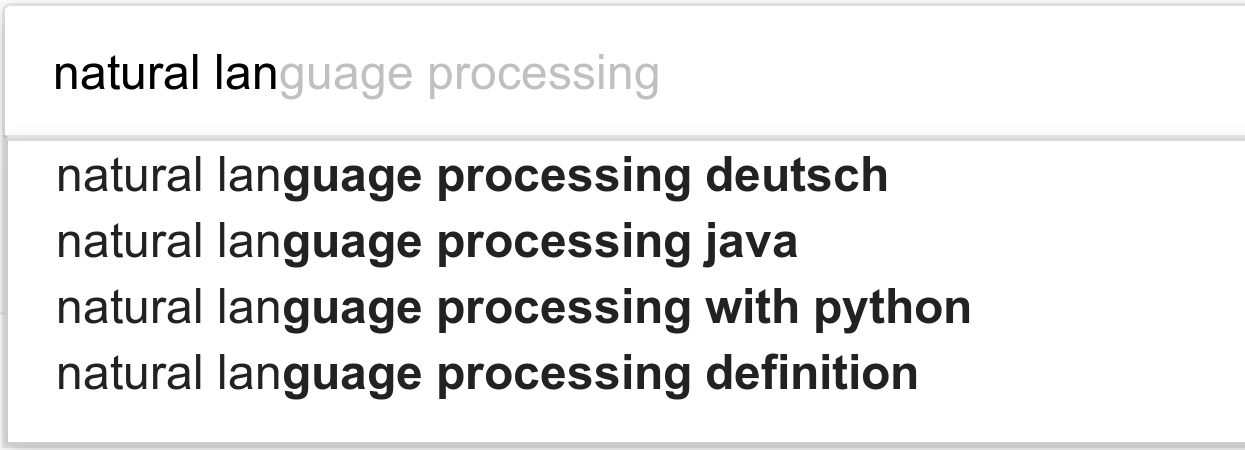
\includegraphics[width=\textwidth]{figures/google-predictive-text-2.png}
  \caption{\label{fig:google-predictive-text}%
    Predictive text on a web search engine in two steps (from google.com).
    Although we do not know exact nature of the language models Google uses,
    n-gram language models we discuss here are definitely a good guess.
    Note that there are two different n-grams models are in action here.
    One predicting the next words based on the previous words,
    and another one predicting the (remaining) characters
    in the word being typed,
    based on previous characters.
  }
\end{marginfigure}

The examples above should be enough for motivating
the n-gram language models,
although there are many more applications of this simple method.
In this chapter we will define them,
discuss important issues and some of the important aspects of estimation,
and mention some of the extensions or advanced usages of n-grams.

\section{Estimating probabilities of n-grams}

N-grams are simply a fixed length sequences of words
(or other units, such as letters).
The length of an n-gram is determined by the `n' in the name.
N-grams of length one, \emph{unigrams}, are simply the words without context.
N-grams of length two and three also have special names,
\emph{bigrams} and \emph{trigrams},
and they are formed by sequences of two and three words respectively.
Larger n-grams are are generally called four-grams, five-grams and so on.

We will use the first articles of the declaration of human rights
for demonstrating what constitutes an n-gram.

%\begin{lstlisting}[language=,basicstyle=\small,breaklines=true]
\begin{tcolorbox}
All human beings are born free and equal in dignity and rights .
They are endowed with reason and conscience and should act towards one another in a spirit of brotherhood .
\end{tcolorbox}
%\end{lstlisting}


\section{Estimating probabilities word sequences}

\section{What is wrong with MLE of n-grams}

\section{Smoothing and back-off}

\subsection{Add-one smoothing}

\section{Extensions}

\section{Rewritten material}

In many natural language applications,
we want to know how likely a particular sequence of units
(words, phonemes, characters, \ldots) is.
For example,
for both practical and theoretical reasons,
we want our computational methods to indicate that 
the sentence (\getfullref{ngram-chomsky.a}) is a likely sentence in English.
The sentence (\getfullref{ngram-chomsky.b}),
on the other hand,
is unlikely
(at least if we discount its usage as a grammatical but nonsense sentence).%
\footnote{%
  All examples except (\getfullref{ngram-chomsky.a}) are from
  \textcite{chomsky1957}.
}
The sentence (\getfullref{ngram-chomsky.c}) is even more unlikely,
it is ungrammatical.
It would probably have never been observed in real language use
if it was not used by Chomsky as an ungrammatical sentence example.
Unlike (\getfullref{ngram-chomsky.e}),
the sentence (\getfullref{ngram-chomsky.d}) is also a common example of
an ungrammatical sentence,
but most native speakers would not have much difficulty to assign
an interpretation (most likely `the child seems to be sleeping') to it
\parencite[p210]{chater2015}.

\pex<ngram-chomsky>
%TODO: better example (the first one)?
  \a<a> Tired little children sleep quietly.
  \a<b> Colorless green ideas sleep furiously.
  \a<c>\ljudge{*} Furiously sleep ideas green colorless.
  \a<d>\ljudge{*} The child seems sleeping.
  \a<e> The book seems interesting.
\xe
Clearly,
we do not want to treat the sentences in (\getref{ngram-chomsky}) the same.
Word ngrams,
or \emph{language models} have been one of the simple but successful methods
for determining which sequences of words are more likely in a language.%
Although their success on capturing
many linguistic dependencies are questionable,
ngram language models have been very useful in practical NLP applications,
ranging from speech recognition to machine translation.
For example,
simple ngram language models like the ones we will discuss can be useful in
\begin{itemize}
  \item spelling correction,
    although all words in \emph{I ate pizza wit spinach}
    are correct words, a language model could easily signal that 
    \emph{I ate pizza wit\textbf{h} spinach} is a more likely sequence.
  \item machine translation
  \item speech recognition
\end{itemize}

\section*{Where to go from here}

\textcite{chen1998} includes a tutorial on most of the smoothing techniques,
followed by an empirical comparison of them.

\section*{Exercises}

\begin{question}
  Which one of the following is a more probably sentence English according to a typical unigram model?
  \begin{itemize}
    \item Furiously sleep ideas green colorless.
    \item Colorless green ideas sleep furiously.
    \item Tired little children sleep quietly. 
    \item the the the the.
  \end{itemize}
\end{question}

\begin{question}
  How do you fix the problem in the previous question?
\end{question}

\begin{question}
  What is perplexity, what does it tell us?
\end{question}

\begin{question}
  Write a python program that calculates bi-gram frequencies for a given corpus.
\end{question}

\begin{question}
  Show that the formula below (to be used earlier),
  corresponds to cross entropy between the distribution defined
  by the n-gram model
  and the MLE estimate of the distribution of words
  in the test corpus.

  \[
    H_{P}(T) = - \frac{1}{\lvert{}T\rvert{}}log_{2}P(T)
  \]
  where P is the probability assigned to a word (sequence)
  by an n-gram model trained on the training corpus,
  T is the test set ($\lvert{}T\rvert{}$ is its size).

\end{question}

%\chapter{\label{chap:morphology}Computational morphology}

\begin{itemize}
  \item Motivation
    \begin{itemize}
      \item Lexicon size - data sparsity
      \item Predictions about unknown words
      \item Parsing / generation
      \item MT 
      \item Spell checking
      \item Information retrieval
      \item TTS
    \end{itemize}
  \item Some definitions
    \begin{itemize}
      \item root - stem - lemma - lexeme
      \item affix - suffix - prefix - infix - circumfix 
      \item reduplication
      \item zero - empty morphemes
      \item inflection vs.\ derivation\\
        tendencies:
        \begin{itemize}
          \item derivation changes category
          \item inflection tends to be paradigmatic
          \item inflection is productive
          \item derivation is lexical, inflection is functional
          \item inflection is semantically regular
          \item inflection is restricted syntactically - agreement etc.
          \item inflection tends to fall on periphery - derivation is more central
          \item derivation is often repeatable
        \end{itemize}
      \item morpheme / morph
      \item compounding 
      \item paradigm 
      \item free - bound morphemes, content vs.\ function
      \item regular and irregular morphology
    \end{itemize}
  \item Morphological typology
    \begin{itemize}
      \item Analytic - synthetic
      \item Isolating - inflectional - agglutinative - templatic
      \item General tendencies: like suffixing more than prefixing, \ldots
    \end{itemize}
  \item Morphological annotation
    \begin{itemize}
      \item Morphology in linguistic glosses
      \item Tagsets in treebanks
      \item Positional tags
      \item Morphological databases - CELEX
    \end{itemize}
  \item Stemming / lemmatization / segmentation
    \begin{itemize}
      \item Compounding / compound splitting
      \item Tries for finding affixes
    \end{itemize}
  \item Tasks in computational morphology
    \begin{itemize}
      \item recognition
      \item analysis
      \item generation
    \end{itemize}
  \item Finite state morphological processing
    \begin{itemize}
      \item FSA
      \item Example: English adjectives (?)
      \item FSA regex relation
      \item Regular languages and Chomsky hierarchy
      \item Deterministic/non-deterministic FSAs
      \item FST 
      \item FSTs as relations - properties
      \item Example FST
      \item Modeling orthographic/phonetic changes: context-sensitive rewrite rules
      \item Porter stemmer
      \item Two-level morphology
      \item Practical examples: Xerox, SFST, \ldots
      \item Weighted FSTs
      \item Weighted FSAs for spelling correction
    \end{itemize}
  \item Statistical learning of morphology
    \begin{itemize}
      \item Learning (re)inflection
      \item Unsupervised methods
    \end{itemize}

\end{itemize}

%\chapter{\label{chap:parsing}Parsing}


In the next lecture, we will discuss \emph{parsing}, 
automatically annotating a given natural language sentence
with a syntactic representation.
Here, we briefly give a general introduction to parsing,
and introduce some terminology and applications.
After which, we will turn our attention
to two major syntactic representations that are used
in the computational linguistics,
\emph{constituency} and \emph{dependency} trees,
and how to parse sentences to produce these representations.%
\footnote{%
  We use these two terms rather in a theory-neutral way
  (as much as possible),
  and focus on the computational processes,
  and practical applications rather than their linguistic adequacy.
  Many linguistic theories of syntax
  make use of ideas from both approaches.
}

\section*{Where to go from here}

\begin{itemize}
  \item \textcite{lease2006} - for applications of parsing
  \item \textcite{muller2016} - for a introduction to different grammar formalisms
\end{itemize}

%\chapter{\label{chap:cf-parsing}Constituency parsing}


\section*{Where to go from here}

%\chapter{\label{chap:dependency-parsing}Dependency parsing}

\section*{Where to go from here}


%\part{NLP applications}
%\chapter{\label{chap:semantics}Computational semantics}

\section*{Where to go from here}

%\chapter{\label{chap:unsupervised-ml}Unsupervised methods in NLP}

\section*{Where to go from here}

%\chapter{\label{chap:text-classification}Text classification}

\section*{Where to go from here}

%\include{document-clustering}
%\include{wsd}
%\chapter{\label{chap:smt}Statistical machine translation}

\section*{Where to go from here}


\printbibliography
\appendix

\end{document}
